\batchmode
\documentclass{article}
\RequirePackage{ifthen}


\usepackage[english]{babel}
\usepackage{geometry,amsmath,amssymb,graphicx,wasysym,textcomp}
\geometry{b4paper}

%
\providecommand{\tmSep}{; }%
\providecommand{\tmaffiliation}[1]{\thanks{\textit{Affiliation:} #1}}%
\providecommand{\tmmathbf}[1]{\ensuremath{\boldsymbol{#1}}}%
\providecommand{\tmop}[1]{\ensuremath{\operatorname{#1}}}%
\providecommand{\tmstrong}[1]{\textbf{#1}} 




\usepackage[dvips]{color}


\pagecolor[gray]{.7}

\usepackage[latin1]{inputenc}



\makeatletter

\makeatletter
\count@=\the\catcode`\_ \catcode`\_=8 
\newenvironment{tex2html_wrap}{}{}%
\catcode`\<=12\catcode`\_=\count@
\newcommand{\providedcommand}[1]{\expandafter\providecommand\csname #1\endcsname}%
\newcommand{\renewedcommand}[1]{\expandafter\providecommand\csname #1\endcsname{}%
  \expandafter\renewcommand\csname #1\endcsname}%
\newcommand{\newedenvironment}[1]{\newenvironment{#1}{}{}\renewenvironment{#1}}%
\let\newedcommand\renewedcommand
\let\renewedenvironment\newedenvironment
\makeatother
\let\mathon=$
\let\mathoff=$
\ifx\AtBeginDocument\undefined \newcommand{\AtBeginDocument}[1]{}\fi
\newbox\sizebox
\setlength{\hoffset}{0pt}\setlength{\voffset}{0pt}
\addtolength{\textheight}{\footskip}\setlength{\footskip}{0pt}
\addtolength{\textheight}{\topmargin}\setlength{\topmargin}{0pt}
\addtolength{\textheight}{\headheight}\setlength{\headheight}{0pt}
\addtolength{\textheight}{\headsep}\setlength{\headsep}{0pt}
\setlength{\textwidth}{349pt}
\newwrite\lthtmlwrite
\makeatletter
\let\realnormalsize=\normalsize
\global\topskip=2sp
\def\preveqno{}\let\real@float=\@float \let\realend@float=\end@float
\def\@float{\let\@savefreelist\@freelist\real@float}
\def\liih@math{\ifmmode$\else\bad@math\fi}
\def\end@float{\realend@float\global\let\@freelist\@savefreelist}
\let\real@dbflt=\@dbflt \let\end@dblfloat=\end@float
\let\@largefloatcheck=\relax
\let\if@boxedmulticols=\iftrue
\def\@dbflt{\let\@savefreelist\@freelist\real@dbflt}
\def\adjustnormalsize{\def\normalsize{\mathsurround=0pt \realnormalsize
 \parindent=0pt\abovedisplayskip=0pt\belowdisplayskip=0pt}%
 \def\phantompar{\csname par\endcsname}\normalsize}%
\def\lthtmltypeout#1{{\let\protect\string \immediate\write\lthtmlwrite{#1}}}%
\newcommand\lthtmlhboxmathA{\adjustnormalsize\setbox\sizebox=\hbox\bgroup\kern.05em }%
\newcommand\lthtmlhboxmathB{\adjustnormalsize\setbox\sizebox=\hbox to\hsize\bgroup\hfill }%
\newcommand\lthtmlvboxmathA{\adjustnormalsize\setbox\sizebox=\vbox\bgroup %
 \let\ifinner=\iffalse \let\)\liih@math }%
\newcommand\lthtmlboxmathZ{\@next\next\@currlist{}{\def\next{\voidb@x}}%
 \expandafter\box\next\egroup}%
\newcommand\lthtmlmathtype[1]{\gdef\lthtmlmathenv{#1}}%
\newcommand\lthtmllogmath{\dimen0\ht\sizebox \advance\dimen0\dp\sizebox
  \ifdim\dimen0>.95\vsize
   \lthtmltypeout{%
*** image for \lthtmlmathenv\space is too tall at \the\dimen0, reducing to .95 vsize ***}%
   \ht\sizebox.95\vsize \dp\sizebox\z@ \fi
  \lthtmltypeout{l2hSize %
:\lthtmlmathenv:\the\ht\sizebox::\the\dp\sizebox::\the\wd\sizebox.\preveqno}}%
\newcommand\lthtmlfigureA[1]{\let\@savefreelist\@freelist
       \lthtmlmathtype{#1}\lthtmlvboxmathA}%
\newcommand\lthtmlpictureA{\bgroup\catcode`\_=8 \lthtmlpictureB}%
\newcommand\lthtmlpictureB[1]{\lthtmlmathtype{#1}\egroup
       \let\@savefreelist\@freelist \lthtmlhboxmathB}%
\newcommand\lthtmlpictureZ[1]{\hfill\lthtmlfigureZ}%
\newcommand\lthtmlfigureZ{\lthtmlboxmathZ\lthtmllogmath\copy\sizebox
       \global\let\@freelist\@savefreelist}%
\newcommand\lthtmldisplayA{\bgroup\catcode`\_=8 \lthtmldisplayAi}%
\newcommand\lthtmldisplayAi[1]{\lthtmlmathtype{#1}\egroup\lthtmlvboxmathA}%
\newcommand\lthtmldisplayB[1]{\edef\preveqno{(\theequation)}%
  \lthtmldisplayA{#1}\let\@eqnnum\relax}%
\newcommand\lthtmldisplayZ{\lthtmlboxmathZ\lthtmllogmath\lthtmlsetmath}%
\newcommand\lthtmlinlinemathA{\bgroup\catcode`\_=8 \lthtmlinlinemathB}
\newcommand\lthtmlinlinemathB[1]{\lthtmlmathtype{#1}\egroup\lthtmlhboxmathA
  \vrule height1.5ex width0pt }%
\newcommand\lthtmlinlineA{\bgroup\catcode`\_=8 \lthtmlinlineB}%
\newcommand\lthtmlinlineB[1]{\lthtmlmathtype{#1}\egroup\lthtmlhboxmathA}%
\newcommand\lthtmlinlineZ{\egroup\expandafter\ifdim\dp\sizebox>0pt %
  \expandafter\centerinlinemath\fi\lthtmllogmath\lthtmlsetinline}
\newcommand\lthtmlinlinemathZ{\egroup\expandafter\ifdim\dp\sizebox>0pt %
  \expandafter\centerinlinemath\fi\lthtmllogmath\lthtmlsetmath}
\newcommand\lthtmlindisplaymathZ{\egroup %
  \centerinlinemath\lthtmllogmath\lthtmlsetmath}
\def\lthtmlsetinline{\hbox{\vrule width.1em \vtop{\vbox{%
  \kern.1em\copy\sizebox}\ifdim\dp\sizebox>0pt\kern.1em\else\kern.3pt\fi
  \ifdim\hsize>\wd\sizebox \hrule depth1pt\fi}}}
\def\lthtmlsetmath{\hbox{\vrule width.1em\kern-.05em\vtop{\vbox{%
  \kern.1em\kern0.8 pt\hbox{\hglue.17em\copy\sizebox\hglue0.8 pt}}\kern.3pt%
  \ifdim\dp\sizebox>0pt\kern.1em\fi \kern0.8 pt%
  \ifdim\hsize>\wd\sizebox \hrule depth1pt\fi}}}
\def\centerinlinemath{%
  \dimen1=\ifdim\ht\sizebox<\dp\sizebox \dp\sizebox\else\ht\sizebox\fi
  \advance\dimen1by.5pt \vrule width0pt height\dimen1 depth\dimen1 
 \dp\sizebox=\dimen1\ht\sizebox=\dimen1\relax}

\def\lthtmlcheckvsize{\ifdim\ht\sizebox<\vsize 
  \ifdim\wd\sizebox<\hsize\expandafter\hfill\fi \expandafter\vfill
  \else\expandafter\vss\fi}%
\providecommand{\selectlanguage}[1]{}%
\makeatletter \tracingstats = 1 
\providecommand{\Beta}{\textrm{B}}
\providecommand{\Mu}{\textrm{M}}
\providecommand{\Kappa}{\textrm{K}}
\providecommand{\Rho}{\textrm{R}}
\providecommand{\Epsilon}{\textrm{E}}
\providecommand{\Chi}{\textrm{X}}
\providecommand{\Iota}{\textrm{J}}
\providecommand{\omicron}{\textrm{o}}
\providecommand{\Zeta}{\textrm{Z}}
\providecommand{\Eta}{\textrm{H}}
\providecommand{\Omicron}{\textrm{O}}
\providecommand{\Nu}{\textrm{N}}
\providecommand{\Tau}{\textrm{T}}
\providecommand{\Alpha}{\textrm{A}}


\begin{document}
\pagestyle{empty}\thispagestyle{empty}\lthtmltypeout{}%
\lthtmltypeout{latex2htmlLength hsize=\the\hsize}\lthtmltypeout{}%
\lthtmltypeout{latex2htmlLength vsize=\the\vsize}\lthtmltypeout{}%
\lthtmltypeout{latex2htmlLength hoffset=\the\hoffset}\lthtmltypeout{}%
\lthtmltypeout{latex2htmlLength voffset=\the\voffset}\lthtmltypeout{}%
\lthtmltypeout{latex2htmlLength topmargin=\the\topmargin}\lthtmltypeout{}%
\lthtmltypeout{latex2htmlLength topskip=\the\topskip}\lthtmltypeout{}%
\lthtmltypeout{latex2htmlLength headheight=\the\headheight}\lthtmltypeout{}%
\lthtmltypeout{latex2htmlLength headsep=\the\headsep}\lthtmltypeout{}%
\lthtmltypeout{latex2htmlLength parskip=\the\parskip}\lthtmltypeout{}%
\lthtmltypeout{latex2htmlLength oddsidemargin=\the\oddsidemargin}\lthtmltypeout{}%
\makeatletter
\if@twoside\lthtmltypeout{latex2htmlLength evensidemargin=\the\evensidemargin}%
\else\lthtmltypeout{latex2htmlLength evensidemargin=\the\oddsidemargin}\fi%
\lthtmltypeout{}%
\makeatother
\setcounter{page}{1}
\onecolumn

% !!! IMAGES START HERE !!!

{\newpage\clearpage
\lthtmlinlinemathA{tex2html_wrap_inline12422}%
$ \rho $%
\lthtmlinlinemathZ
\lthtmlcheckvsize\clearpage}

{\newpage\clearpage
\lthtmlinlinemathA{tex2html_wrap_inline12426}%
$ \xi $%
\lthtmlinlinemathZ
\lthtmlcheckvsize\clearpage}

{\newpage\clearpage
\lthtmlinlinemathA{tex2html_wrap_inline12430}%
$ \nabla \Psi $%
\lthtmlinlinemathZ
\lthtmlcheckvsize\clearpage}

{\newpage\clearpage
\lthtmlinlinemathA{tex2html_wrap_inline12434}%
$ B_0 \times \nabla \Psi $%
\lthtmlinlinemathZ
\lthtmlcheckvsize\clearpage}

{\newpage\clearpage
\lthtmlinlinemathA{tex2html_wrap_inline12438}%
$ B_0$%
\lthtmlinlinemathZ
\lthtmlcheckvsize\clearpage}

{\newpage\clearpage
\lthtmlinlinemathA{tex2html_wrap_inline12454}%
$ (P_1, \xi _{\psi }, \xi _s, \nabla \cdot \xi )$%
\lthtmlinlinemathZ
\lthtmlcheckvsize\clearpage}

{\newpage\clearpage
\lthtmlinlinemathA{tex2html_wrap_inline12460}%
$ \theta $%
\lthtmlinlinemathZ
\lthtmlcheckvsize\clearpage}

{\newpage\clearpage
\lthtmlinlinemathA{tex2html_wrap_inline12462}%
$ \zeta $%
\lthtmlinlinemathZ
\lthtmlcheckvsize\clearpage}

{\newpage\clearpage
\lthtmlinlinemathA{tex2html_wrap_inline12472}%
$ C$%
\lthtmlinlinemathZ
\lthtmlcheckvsize\clearpage}

{\newpage\clearpage
\lthtmlinlinemathA{tex2html_wrap_inline12474}%
$ D$%
\lthtmlinlinemathZ
\lthtmlcheckvsize\clearpage}

{\newpage\clearpage
\lthtmlinlinemathA{tex2html_wrap_inline12476}%
$ E$%
\lthtmlinlinemathZ
\lthtmlcheckvsize\clearpage}

{\newpage\clearpage
\lthtmlinlinemathA{tex2html_wrap_inline12478}%
$ F$%
\lthtmlinlinemathZ
\lthtmlcheckvsize\clearpage}

{\newpage\clearpage
\lthtmlinlinemathA{tex2html_wrap_inline12490}%
$ n = 1$%
\lthtmlinlinemathZ
\lthtmlcheckvsize\clearpage}

{\newpage\clearpage
\lthtmlinlinemathA{tex2html_wrap_inline12492}%
$ m = 0, 1, 2, 3, 4$%
\lthtmlinlinemathZ
\lthtmlcheckvsize\clearpage}

{\newpage\clearpage
\lthtmlinlinemathA{tex2html_wrap_inline12494}%
$ 5$%
\lthtmlinlinemathZ
\lthtmlcheckvsize\clearpage}

{\newpage\clearpage
\lthtmlinlinemathA{tex2html_wrap_inline12496}%
$ \mathcal  {J}$%
\lthtmlinlinemathZ
\lthtmlcheckvsize\clearpage}

{\newpage\clearpage
\lthtmlinlinemathA{tex2html_wrap_inline12512}%
$ m = 2, 3, 4, 5$%
\lthtmlinlinemathZ
\lthtmlcheckvsize\clearpage}

{\newpage\clearpage
\lthtmlinlinemathA{tex2html_wrap_inline12516}%
$ f = 297 \ensuremath  {\operatorname  {kHz}}$%
\lthtmlinlinemathZ
\lthtmlcheckvsize\clearpage}

{\newpage\clearpage
\lthtmlinlinemathA{tex2html_wrap_inline12532}%
$ m = 2$%
\lthtmlinlinemathZ
\lthtmlcheckvsize\clearpage}

{\newpage\clearpage
\lthtmlinlinemathA{tex2html_wrap_inline12534}%
$ m = 5$%
\lthtmlinlinemathZ
\lthtmlcheckvsize\clearpage}

{\newpage\clearpage
\lthtmlinlinemathA{tex2html_wrap_inline12548}%
$ f = 93 \ensuremath  {\operatorname  {kHz}}$%
\lthtmlinlinemathZ
\lthtmlcheckvsize\clearpage}

{\newpage\clearpage
\lthtmlinlinemathA{tex2html_wrap_inline12550}%
$ m = 3$%
\lthtmlinlinemathZ
\lthtmlcheckvsize\clearpage}

{\newpage\clearpage
\lthtmlinlinemathA{tex2html_wrap_inline12552}%
$ m = 4$%
\lthtmlinlinemathZ
\lthtmlcheckvsize\clearpage}

{\newpage\clearpage
\lthtmlinlinemathA{tex2html_wrap_inline12584}%
$ f = 102 \ensuremath  {\operatorname  {kHz}}$%
\lthtmlinlinemathZ
\lthtmlcheckvsize\clearpage}

{\newpage\clearpage
\lthtmlinlinemathA{tex2html_wrap_inline12610}%
$ S$%
\lthtmlinlinemathZ
\lthtmlcheckvsize\clearpage}

{\newpage\clearpage
\lthtmlinlinemathA{tex2html_wrap_inline12616}%
$ {\textmu }_0 \sigma $%
\lthtmlinlinemathZ
\lthtmlcheckvsize\clearpage}

{\newpage\clearpage
\lthtmlinlinemathA{tex2html_wrap_inline12638}%
$ \beta $%
\lthtmlinlinemathZ
\lthtmlcheckvsize\clearpage}

{\newpage\clearpage
\lthtmlinlinemathA{tex2html_wrap_inline12642}%
$ [- 10 : 10]$%
\lthtmlinlinemathZ
\lthtmlcheckvsize\clearpage}

{\newpage\clearpage
\lthtmlinlinemathA{tex2html_wrap_inline12648}%
$ [- 10, 10]$%
\lthtmlinlinemathZ
\lthtmlcheckvsize\clearpage}

{\newpage\clearpage
\lthtmlinlinemathA{tex2html_wrap_inline12650}%
$ [- 15, 15]$%
\lthtmlinlinemathZ
\lthtmlcheckvsize\clearpage}

{\newpage\clearpage
\lthtmlinlinemathA{tex2html_wrap_inline12656}%
$ n = 4$%
\lthtmlinlinemathZ
\lthtmlcheckvsize\clearpage}

{\newpage\clearpage
\lthtmlinlinemathA{tex2html_wrap_inline12658}%
$ [- 15, 20]$%
\lthtmlinlinemathZ
\lthtmlcheckvsize\clearpage}

{\newpage\clearpage
\lthtmlinlinemathA{tex2html_wrap_inline12662}%
$ \kappa _{\psi }$%
\lthtmlinlinemathZ
\lthtmlcheckvsize\clearpage}

{\newpage\clearpage
\lthtmlinlinemathA{tex2html_wrap_inline12676}%
$ f = 101 \ensuremath  {\operatorname  {kHz}}$%
\lthtmlinlinemathZ
\lthtmlcheckvsize\clearpage}

{\newpage\clearpage
\lthtmlinlinemathA{tex2html_wrap_inline12678}%
$ m = 1$%
\lthtmlinlinemathZ
\lthtmlcheckvsize\clearpage}

{\newpage\clearpage
\lthtmlinlinemathA{tex2html_wrap_inline12702}%
$ \kappa _s$%
\lthtmlinlinemathZ
\lthtmlcheckvsize\clearpage}

{\newpage\clearpage
\lthtmlinlinemathA{tex2html_wrap_inline12716}%
$ f = 61.91 \ensuremath  {\operatorname  {kHz}}$%
\lthtmlinlinemathZ
\lthtmlcheckvsize\clearpage}

{\newpage\clearpage
\lthtmlinlinemathA{tex2html_wrap_inline12756}%
$ f = 130 \ensuremath  {\operatorname  {kHz}}$%
\lthtmlinlinemathZ
\lthtmlcheckvsize\clearpage}

{\newpage\clearpage
\lthtmlinlinemathA{tex2html_wrap_inline12778}%
$ f = 216 \ensuremath  {\operatorname  {kHz}}$%
\lthtmlinlinemathZ
\lthtmlcheckvsize\clearpage}

{\newpage\clearpage
\lthtmlinlinemathA{tex2html_wrap_inline12798}%
$ f = 330 \ensuremath  {\operatorname  {kHz}}$%
\lthtmlinlinemathZ
\lthtmlcheckvsize\clearpage}

{\newpage\clearpage
\lthtmlinlinemathA{tex2html_wrap_inline12802}%
$ m = 7$%
\lthtmlinlinemathZ
\lthtmlcheckvsize\clearpage}

{\newpage\clearpage
\lthtmlinlinemathA{tex2html_wrap_inline12804}%
$ m = [- 10, 10]$%
\lthtmlinlinemathZ
\lthtmlcheckvsize\clearpage}

{\newpage\clearpage
\lthtmlinlinemathA{tex2html_wrap_inline12832}%
$ | \nabla \Psi |^2 S$%
\lthtmlinlinemathZ
\lthtmlcheckvsize\clearpage}

{\newpage\clearpage
\lthtmlinlinemathA{tex2html_wrap_inline12842}%
$ d q / d \psi $%
\lthtmlinlinemathZ
\lthtmlcheckvsize\clearpage}

{\newpage\clearpage
\lthtmlinlinemathA{tex2html_wrap_inline12844}%
$ - \delimiter "426830A S \delimiter "526930B \DOTSI \intop \ilimits@ _0^{2 \pi } \mathcal  {J}d \theta / (2 \pi )$%
\lthtmlinlinemathZ
\lthtmlcheckvsize\clearpage}

{\newpage\clearpage
\lthtmlinlinemathA{tex2html_wrap_inline12846}%
$ \overline  {\Psi }$%
\lthtmlinlinemathZ
\lthtmlcheckvsize\clearpage}

{\newpage\clearpage
\lthtmlinlinemathA{tex2html_wrap_inline12852}%
$ C_{22}$%
\lthtmlinlinemathZ
\lthtmlcheckvsize\clearpage}

{\newpage\clearpage
\lthtmlinlinemathA{tex2html_wrap_inline12858}%
$ k_{\parallel }$%
\lthtmlinlinemathZ
\lthtmlcheckvsize\clearpage}

{\newpage\clearpage
\lthtmlinlinemathA{tex2html_wrap_inline12860}%
$ k_{\theta }$%
\lthtmlinlinemathZ
\lthtmlcheckvsize\clearpage}

{\newpage\clearpage
\lthtmlinlinemathA{tex2html_wrap_inline12878}%
$ \varphi = 0$%
\lthtmlinlinemathZ
\lthtmlcheckvsize\clearpage}

{\newpage\clearpage
\lthtmlinlinemathA{tex2html_wrap_inline12882}%
$ r_s = 0.5$%
\lthtmlinlinemathZ
\lthtmlcheckvsize\clearpage}

{\newpage\clearpage
\lthtmlinlinemathA{tex2html_wrap_inline12884}%
$ \Delta = \sqrt  {0.02}$%
\lthtmlinlinemathZ
\lthtmlcheckvsize\clearpage}

{\newpage\clearpage
\lthtmlinlinemathA{tex2html_wrap_inline12886}%
$ t = 0$%
\lthtmlinlinemathZ
\lthtmlcheckvsize\clearpage}

{\newpage\clearpage
\lthtmlinlinemathA{tex2html_wrap_inline12888}%
$ \alpha = 0$%
\lthtmlinlinemathZ
\lthtmlcheckvsize\clearpage}

{\newpage\clearpage
\lthtmlinlinemathA{tex2html_wrap_inline12890}%
$ \alpha $%
\lthtmlinlinemathZ
\lthtmlcheckvsize\clearpage}

{\newpage\clearpage
\lthtmlinlinemathA{tex2html_wrap_inline12910}%
$ m_1 = m_2 - 1 = 4$%
\lthtmlinlinemathZ
\lthtmlcheckvsize\clearpage}

{\newpage\clearpage
\lthtmlinlinemathA{tex2html_wrap_inline12924}%
$ (B \times \nabla \psi ) \cdot \nabla \left ( \frac  {1}{B^2} \right ) = - 2 \kappa \cdot (B \times \nabla \psi ) / B^2$%
\lthtmlinlinemathZ
\lthtmlcheckvsize\clearpage}

\stepcounter{section}
{\newpage\clearpage
\lthtmlinlinemathA{tex2html_wrap_inline12930}%
$ \mathbf{u}$%
\lthtmlinlinemathZ
\lthtmlcheckvsize\clearpage}

{\newpage\clearpage
\lthtmlinlinemathA{tex2html_wrap_indisplay12932}%
$\displaystyle \rho \left( \frac{\partial \mathbf{u}}{\partial t}   +\mathbf{u} \cdot \nabla \mathbf{u} \right) = \rho_q \mathbf{E}- \nabla p   +\mathbf{J} \times \mathbf{B},$%
\lthtmlindisplaymathZ
\lthtmlcheckvsize\clearpage}

{\newpage\clearpage
\lthtmlinlinemathA{tex2html_wrap_inline12936}%
$ \rho_q$%
\lthtmlinlinemathZ
\lthtmlcheckvsize\clearpage}

{\newpage\clearpage
\lthtmlinlinemathA{tex2html_wrap_inline12938}%
$ p$%
\lthtmlinlinemathZ
\lthtmlcheckvsize\clearpage}

{\newpage\clearpage
\lthtmlinlinemathA{tex2html_wrap_inline12940}%
$ \mathbf{J}$%
\lthtmlinlinemathZ
\lthtmlcheckvsize\clearpage}

{\newpage\clearpage
\lthtmlinlinemathA{tex2html_wrap_inline12942}%
$ \mathbf{E}$%
\lthtmlinlinemathZ
\lthtmlcheckvsize\clearpage}

{\newpage\clearpage
\lthtmlinlinemathA{tex2html_wrap_inline12944}%
$ \mathbf{B}$%
\lthtmlinlinemathZ
\lthtmlcheckvsize\clearpage}

{\newpage\clearpage
\lthtmlinlinemathA{tex2html_wrap_indisplay12948}%
$\displaystyle \frac{\partial \rho}{\partial t} + \nabla \cdot (\rho \mathbf{u}) = 0.$%
\lthtmlindisplaymathZ
\lthtmlcheckvsize\clearpage}

{\newpage\clearpage
\lthtmlinlinemathA{tex2html_wrap_indisplay12952}%
$\displaystyle \frac{d}{d t} (p \rho^{- \gamma}) = 0,$%
\lthtmlindisplaymathZ
\lthtmlcheckvsize\clearpage}

{\newpage\clearpage
\lthtmlinlinemathA{tex2html_wrap_inline12954}%
$ \gamma$%
\lthtmlinlinemathZ
\lthtmlcheckvsize\clearpage}

{\newpage\clearpage
\lthtmlinlinemathA{tex2html_wrap_indisplay12958}%
$\displaystyle \frac{\partial \mathbf{B}}{\partial t} = - \nabla \times   \mathbf{E}.$%
\lthtmlindisplaymathZ
\lthtmlcheckvsize\clearpage}

{\newpage\clearpage
\lthtmlinlinemathA{tex2html_wrap_indisplay12962}%
$\displaystyle \mathbf{J}= \frac{1}{{\textmu}_0} \nabla \times \mathbf{B}$%
\lthtmlindisplaymathZ
\lthtmlcheckvsize\clearpage}

{\newpage\clearpage
\lthtmlinlinemathA{tex2html_wrap_indisplay12966}%
$\displaystyle \mathbf{E}= -\mathbf{u} \times \mathbf{B}+ \eta \mathbf{J}.$%
\lthtmlindisplaymathZ
\lthtmlcheckvsize\clearpage}

{\newpage\clearpage
\lthtmlinlinemathA{tex2html_wrap_indisplay12970}%
$\displaystyle \rho_q = \varepsilon_0 \nabla \cdot \mathbf{E}.$%
\lthtmlindisplaymathZ
\lthtmlcheckvsize\clearpage}

{\newpage\clearpage
\lthtmlinlinemathA{tex2html_wrap_indisplay12986}%
$\displaystyle \nabla \cdot \mathbf{B}= 0.$%
\lthtmlindisplaymathZ
\lthtmlcheckvsize\clearpage}

{\newpage\clearpage
\lthtmlinlinemathA{tex2html_wrap_inline12996}%
$ \frac{\partial \mathbf{B}}{\partial t} = - \nabla \times (-\mathbf{u}
  \times \mathbf{B}+ \eta (\nabla \times \mathbf{B}) /{\textmu}_0) = \nabla
  \times (\mathbf{u} \times \mathbf{B}) + \eta \nabla^2
  \mathbf{B}/{\textmu}_0$%
\lthtmlinlinemathZ
\lthtmlcheckvsize\clearpage}

{\newpage\clearpage
\lthtmlinlinemathA{tex2html_wrap_inline12998}%
$ \rho \left( \frac{\partial \mathbf{u}}{\partial t} +\mathbf{u} \cdot \nabla
  \mathbf{u} \right) = \rho_q \mathbf{E}- \nabla p + (\nabla \times
  \mathbf{B}) /{\textmu}_0 \times \mathbf{B}$%
\lthtmlinlinemathZ
\lthtmlcheckvsize\clearpage}

{\newpage\clearpage
\lthtmlinlinemathA{tex2html_wrap_inline13000}%
$ \frac{\partial \rho}{\partial t} + \nabla \cdot (\rho \mathbf{u}) = 0$%
\lthtmlinlinemathZ
\lthtmlcheckvsize\clearpage}

{\newpage\clearpage
\lthtmlinlinemathA{tex2html_wrap_inline13002}%
$ \frac{d}{d t} (p \rho^{- \gamma}) = 0$%
\lthtmlinlinemathZ
\lthtmlcheckvsize\clearpage}

{\newpage\clearpage
\lthtmlinlinemathA{tex2html_wrap_inline13004}%
$ \nabla \cdot \mathbf{B}= 0$%
\lthtmlinlinemathZ
\lthtmlcheckvsize\clearpage}

{\newpage\clearpage
\lthtmlinlinemathA{tex2html_wrap_inline13006}%
$ \mathbf{E}= \eta (\nabla \times \mathbf{B}) /{\textmu}_0 -\mathbf{u} \times
  \mathbf{B}$%
\lthtmlinlinemathZ
\lthtmlcheckvsize\clearpage}

{\newpage\clearpage
\lthtmlinlinemathA{tex2html_wrap_inline13008}%
$ \mathbf{J}= (\nabla \times \mathbf{B}) /{\textmu}_0$%
\lthtmlinlinemathZ
\lthtmlcheckvsize\clearpage}

{\newpage\clearpage
\lthtmlinlinemathA{tex2html_wrap_inline13010}%
$ \rho_q = \varepsilon_0 \nabla \cdot \mathbf{E}$%
\lthtmlinlinemathZ
\lthtmlcheckvsize\clearpage}

{\newpage\clearpage
\lthtmlinlinemathA{tex2html_wrap_inline13012}%
$ \rho_q \mathbf{E}$%
\lthtmlinlinemathZ
\lthtmlcheckvsize\clearpage}

\stepcounter{subsection}
{\newpage\clearpage
\lthtmlinlinemathA{tex2html_wrap_indisplay13015}%
$\displaystyle \frac{\partial \nabla \cdot \mathbf{B}}{\partial t} = - \nabla \cdot (\nabla   \times \mathbf{E}) = 0,$%
\lthtmlindisplaymathZ
\lthtmlcheckvsize\clearpage}

{\newpage\clearpage
\lthtmlinlinemathA{tex2html_wrap_indisplay13019}%
$\displaystyle \nabla \cdot \mathbf{J}= 0.$%
\lthtmlindisplaymathZ
\lthtmlcheckvsize\clearpage}

{\newpage\clearpage
\lthtmlinlinemathA{tex2html_wrap_indisplay13022}%
$\displaystyle \rho_q$%
\lthtmlindisplaymathZ
\lthtmlcheckvsize\clearpage}

{\newpage\clearpage
\lthtmlinlinemathA{tex2html_wrap_indisplay13024}%
$\displaystyle \equiv$%
\lthtmlindisplaymathZ
\lthtmlcheckvsize\clearpage}

{\newpage\clearpage
\lthtmlinlinemathA{tex2html_wrap_indisplay13026}%
$\displaystyle \varepsilon_0 \nabla \cdot \mathbf{E}$%
\lthtmlindisplaymathZ
\lthtmlcheckvsize\clearpage}

{\newpage\clearpage
\lthtmlinlinemathA{tex2html_wrap_indisplay13028}%
$\displaystyle =$%
\lthtmlindisplaymathZ
\lthtmlcheckvsize\clearpage}

{\newpage\clearpage
\lthtmlinlinemathA{tex2html_wrap_indisplay13030}%
$\displaystyle \varepsilon_0 \nabla \cdot (\eta \mathbf{J}-\mathbf{u} \times
\mathbf{B}) .$%
\lthtmlindisplaymathZ
\lthtmlcheckvsize\clearpage}

{\newpage\clearpage
\lthtmlinlinemathA{tex2html_wrap_inline13034}%
$ \partial \rho_q / \partial t \neq 0$%
\lthtmlinlinemathZ
\lthtmlcheckvsize\clearpage}

{\newpage\clearpage
\lthtmlinlinemathA{tex2html_wrap_inline13036}%
$ \partial \mathbf{E}/
\partial t$%
\lthtmlinlinemathZ
\lthtmlcheckvsize\clearpage}

\stepcounter{subsection}
{\newpage\clearpage
\lthtmlinlinemathA{tex2html_wrap_indisplay13045}%
$\displaystyle \mathbf{E}+\mathbf{u} \times \mathbf{B}- \eta \mathbf{J}=   \frac{1}{e n} \mathbf{J} \times \mathbf{B}- \frac{1}{e n} \nabla \cdot   \mathbf{P}_e + \frac{m_e}{n e^2}  \left[ \frac{\partial \mathbf{J}}{\partial   t} + \nabla \cdot (\mathbf{J}\mathbf{u}+\mathbf{u}\mathbf{J}) \right],$%
\lthtmlindisplaymathZ
\lthtmlcheckvsize\clearpage}

{\newpage\clearpage
\lthtmlinlinemathA{tex2html_wrap_inline13061}%
$ \partial \mathbf{J}/
\partial t$%
\lthtmlinlinemathZ
\lthtmlcheckvsize\clearpage}

\stepcounter{subsection}
{\newpage\clearpage
\lthtmlinlinemathA{tex2html_wrap_indisplay13080}%
$\displaystyle \frac{d p}{d t} \rho^{- \gamma} - \gamma \rho^{- (\gamma + 1)} p \frac{d   \rho}{d t} = 0,$%
\lthtmlindisplaymathZ
\lthtmlcheckvsize\clearpage}

{\newpage\clearpage
\lthtmlinlinemathA{tex2html_wrap_indisplay13082}%
$\displaystyle \frac{d p}{d t} = \gamma \frac{p}{\rho} \frac{d \rho}{d t}$%
\lthtmlindisplaymathZ
\lthtmlcheckvsize\clearpage}

{\newpage\clearpage
\lthtmlinlinemathA{tex2html_wrap_indisplay13084}%
$\displaystyle \frac{\partial p}{\partial t} +\mathbf{u} \cdot \nabla p = \gamma   \frac{p}{\rho} \left( \frac{\partial \rho}{\partial t} +\mathbf{u} \cdot   \nabla \rho \right)$%
\lthtmlindisplaymathZ
\lthtmlcheckvsize\clearpage}

{\newpage\clearpage
\lthtmlinlinemathA{tex2html_wrap_indisplay13088}%
$\displaystyle \frac{\partial p}{\partial t} = - \gamma p \nabla \cdot   \mathbf{u}-\mathbf{u} \cdot \nabla p.$%
\lthtmlindisplaymathZ
\lthtmlcheckvsize\clearpage}

{\newpage\clearpage
\lthtmlinlinemathA{tex2html_wrap_inline13090}%
$ \gamma = 1$%
\lthtmlinlinemathZ
\lthtmlcheckvsize\clearpage}

{\newpage\clearpage
\lthtmlinlinemathA{tex2html_wrap_indisplay13092}%
$\displaystyle \frac{\partial p}{\partial t} = - \nabla \cdot (p\mathbf{u}) .$%
\lthtmlindisplaymathZ
\lthtmlcheckvsize\clearpage}

\stepcounter{subsection}
{\newpage\clearpage
\lthtmlinlinemathA{tex2html_wrap_indisplay13103}%
$\displaystyle \frac{\partial \mathbf{B}}{\partial t} = \nabla \times   (\mathbf{u} \times \mathbf{B}) + \eta \nabla^2 \mathbf{B}/{\textmu}_0,$%
\lthtmlindisplaymathZ
\lthtmlcheckvsize\clearpage}

{\newpage\clearpage
\lthtmlinlinemathA{tex2html_wrap_indisplay13105}%
$\displaystyle \rho \left( \frac{\partial \mathbf{u}}{\partial t} +\mathbf{u} \cdot \nabla   \mathbf{u} \right) = - \nabla p + (\nabla \times \mathbf{B}) /{\textmu}_0   \times \mathbf{B},$%
\lthtmlindisplaymathZ
\lthtmlcheckvsize\clearpage}

{\newpage\clearpage
\lthtmlinlinemathA{tex2html_wrap_indisplay13107}%
$\displaystyle \frac{\partial p}{\partial t} = - \gamma p \nabla \cdot   \mathbf{u}-\mathbf{u} \cdot \nabla p,$%
\lthtmlindisplaymathZ
\lthtmlcheckvsize\clearpage}

{\newpage\clearpage
\lthtmlinlinemathA{tex2html_wrap_indisplay13109}%
$\displaystyle \frac{\partial \rho}{\partial t} = - \rho \nabla \cdot \mathbf{u}-\mathbf{u}   \cdot \nabla \rho .$%
\lthtmlindisplaymathZ
\lthtmlcheckvsize\clearpage}

{\newpage\clearpage
\lthtmlinlinemathA{tex2html_wrap_inline13111}%
$ \eta$%
\lthtmlinlinemathZ
\lthtmlcheckvsize\clearpage}

{\newpage\clearpage
\lthtmlinlinemathA{tex2html_wrap_inline13113}%
$ \eta
= 0$%
\lthtmlinlinemathZ
\lthtmlcheckvsize\clearpage}

\stepcounter{section}
{\newpage\clearpage
\lthtmlinlinemathA{tex2html_wrap_inline13116}%
$ \mathbf{u}_0$%
\lthtmlinlinemathZ
\lthtmlcheckvsize\clearpage}

{\newpage\clearpage
\lthtmlinlinemathA{tex2html_wrap_inline13118}%
$ \mathbf{B}_0$%
\lthtmlinlinemathZ
\lthtmlcheckvsize\clearpage}

{\newpage\clearpage
\lthtmlinlinemathA{tex2html_wrap_inline13120}%
$ p_0$%
\lthtmlinlinemathZ
\lthtmlcheckvsize\clearpage}

{\newpage\clearpage
\lthtmlinlinemathA{tex2html_wrap_inline13122}%
$ \rho_0$%
\lthtmlinlinemathZ
\lthtmlcheckvsize\clearpage}

{\newpage\clearpage
\lthtmlinlinemathA{tex2html_wrap_inline13124}%
$ \mathbf{u}_1$%
\lthtmlinlinemathZ
\lthtmlcheckvsize\clearpage}

{\newpage\clearpage
\lthtmlinlinemathA{tex2html_wrap_inline13126}%
$ \mathbf{B}_1$%
\lthtmlinlinemathZ
\lthtmlcheckvsize\clearpage}

{\newpage\clearpage
\lthtmlinlinemathA{tex2html_wrap_inline13128}%
$ p_1$%
\lthtmlinlinemathZ
\lthtmlcheckvsize\clearpage}

{\newpage\clearpage
\lthtmlinlinemathA{tex2html_wrap_inline13130}%
$ \rho_1$%
\lthtmlinlinemathZ
\lthtmlcheckvsize\clearpage}

{\newpage\clearpage
\lthtmlinlinemathA{tex2html_wrap_inline13132}%
$ \mathbf{u}_0 = 0$%
\lthtmlinlinemathZ
\lthtmlcheckvsize\clearpage}

{\newpage\clearpage
\lthtmlinlinemathA{tex2html_wrap_indisplay13134}%
$\displaystyle \frac{\partial p_1}{\partial t} = - \gamma p_0 \nabla \cdot   \mathbf{u}_1 -\mathbf{u}_1 \cdot \nabla p_0 .$%
\lthtmlindisplaymathZ
\lthtmlcheckvsize\clearpage}

{\newpage\clearpage
\lthtmlinlinemathA{tex2html_wrap_indisplay13136}%
$\displaystyle \rho_0 \frac{\partial \mathbf{u}_1}{\partial t} = - \nabla   p_1 +{\textmu}_0^{- 1} (\nabla \times \mathbf{B}_1) \times \mathbf{B}_0   +{\textmu}_0^{- 1} (\nabla \times \mathbf{B}_0) \times \mathbf{B}_1 .$%
\lthtmlindisplaymathZ
\lthtmlcheckvsize\clearpage}

{\newpage\clearpage
\lthtmlinlinemathA{tex2html_wrap_indisplay13138}%
$\displaystyle \frac{\partial \mathbf{B}_1}{\partial t} = \nabla \times   (\mathbf{u}_1 \times \mathbf{B}_0) .$%
\lthtmlindisplaymathZ
\lthtmlcheckvsize\clearpage}

{\newpage\clearpage
\lthtmlinlinemathA{tex2html_wrap_indisplay13148}%
$\displaystyle \frac{\partial \rho_1}{\partial t} = - \rho_0 \nabla \cdot \mathbf{u}_1   -\mathbf{u}_1 \cdot \nabla \rho_0$%
\lthtmlindisplaymathZ
\lthtmlcheckvsize\clearpage}

\stepcounter{subsection}
{\newpage\clearpage
\lthtmlinlinemathA{tex2html_wrap_inline13155}%
$ \ensuremath{\boldsymbol{\xi}}$%
\lthtmlinlinemathZ
\lthtmlcheckvsize\clearpage}

{\newpage\clearpage
\lthtmlinlinemathA{tex2html_wrap_indisplay13157}%
$\displaystyle \mathbf{u}_1 = \frac{\partial \ensuremath{\boldsymbol{\xi}}}{\partial t} .$%
\lthtmlindisplaymathZ
\lthtmlcheckvsize\clearpage}

{\newpage\clearpage
\lthtmlinlinemathA{tex2html_wrap_indisplay13161}%
$\displaystyle \frac{\partial \mathbf{B}_1}{\partial t} =   \frac{\partial}{\partial t} [\nabla \times (\ensuremath{\boldsymbol{\xi}} \times   \mathbf{B}_0)] .$%
\lthtmlindisplaymathZ
\lthtmlcheckvsize\clearpage}

{\newpage\clearpage
\lthtmlinlinemathA{tex2html_wrap_indisplay13163}%
$\displaystyle \frac{\partial p_1}{\partial t} = \frac{\partial}{\partial   t} [-\ensuremath{\boldsymbol{\xi}} \cdot \nabla p_0 - \gamma p_0 \nabla \cdot   \ensuremath{\boldsymbol{\xi}}] .$%
\lthtmlindisplaymathZ
\lthtmlcheckvsize\clearpage}

{\newpage\clearpage
\lthtmlinlinemathA{tex2html_wrap_indisplay13165}%
$\displaystyle \rho_0 \frac{\partial^2 \ensuremath{\boldsymbol{\xi}}}{\partial t^2} = -   \nabla p_1 +{\textmu}_0^{- 1} (\nabla \times \mathbf{B}_1) \times   \mathbf{B}_0 +{\textmu}_0^{- 1} (\nabla \times \mathbf{B}_0) \times   \mathbf{B}_1 .$%
\lthtmlindisplaymathZ
\lthtmlcheckvsize\clearpage}

\stepcounter{subsection}
{\newpage\clearpage
\lthtmlinlinemathA{tex2html_wrap_indisplay13174}%
$\displaystyle h (t) = \frac{1}{2 \pi} \int_{- \infty}^{\infty} \hat{h}   (\omega) e^{- i \omega t} d \omega,$%
\lthtmlindisplaymathZ
\lthtmlcheckvsize\clearpage}

{\newpage\clearpage
\lthtmlinlinemathA{tex2html_wrap_inline13176}%
$ \hat{h} (\omega)$%
\lthtmlinlinemathZ
\lthtmlcheckvsize\clearpage}

{\newpage\clearpage
\lthtmlinlinemathA{tex2html_wrap_inline13178}%
$ h (t)$%
\lthtmlinlinemathZ
\lthtmlcheckvsize\clearpage}

{\newpage\clearpage
\lthtmlinlinemathA{tex2html_wrap_indisplay13180}%
$\displaystyle \hat{h} (\omega) = \int_{- \infty}^{\infty} h (t) e^{i \omega t} d t,$%
\lthtmlindisplaymathZ
\lthtmlcheckvsize\clearpage}

{\newpage\clearpage
\lthtmlinlinemathA{tex2html_wrap_indisplay13182}%
$\displaystyle \int_{- \infty}^{\infty} \frac{\partial}{\partial t} h (t)   e^{i \omega t} d t = - i \omega \hat{h} (\omega),$%
\lthtmlindisplaymathZ
\lthtmlcheckvsize\clearpage}

{\newpage\clearpage
\lthtmlinlinemathA{tex2html_wrap_indisplay13184}%
$\displaystyle \int_{- \infty}^{\infty} \frac{\partial^2}{\partial t^2} h   (t) e^{i \omega t} d t = - \omega^2 \hat{h} (\omega) .$%
\lthtmlindisplaymathZ
\lthtmlcheckvsize\clearpage}

{\newpage\clearpage
\lthtmlinlinemathA{tex2html_wrap_indisplay13186}%
$\displaystyle - \omega^2 \rho_0 \hat{\ensuremath{\boldsymbol{\xi}}} = - \nabla \hat{p}_1   +{\textmu}_0^{- 1} (\nabla \times \hat{\mathbf{B}}_1) \times \mathbf{B}_0   +{\textmu}_0^{- 1} (\nabla \times \mathbf{B}_0) \times \hat{\mathbf{B}}_1,$%
\lthtmlindisplaymathZ
\lthtmlcheckvsize\clearpage}

{\newpage\clearpage
\lthtmlinlinemathA{tex2html_wrap_indisplay13188}%
$\displaystyle \hat{p}_1 = - \hat{\ensuremath{\boldsymbol{\xi}}} \cdot \nabla p_0 - \gamma   p_0 \nabla \cdot \hat{\ensuremath{\boldsymbol{\xi}}},$%
\lthtmlindisplaymathZ
\lthtmlcheckvsize\clearpage}

{\newpage\clearpage
\lthtmlinlinemathA{tex2html_wrap_indisplay13190}%
$\displaystyle \hat{\mathbf{B}}_1 = \nabla \times (\hat{\ensuremath{\boldsymbol{\xi}}}   \times \mathbf{B}_0),$%
\lthtmlindisplaymathZ
\lthtmlcheckvsize\clearpage}

{\newpage\clearpage
\lthtmlinlinemathA{tex2html_wrap_inline13192}%
$ \hat{\ensuremath{\boldsymbol{\xi}}}$%
\lthtmlinlinemathZ
\lthtmlcheckvsize\clearpage}

{\newpage\clearpage
\lthtmlinlinemathA{tex2html_wrap_inline13194}%
$ \hat{\mathbf{B}}_1$%
\lthtmlinlinemathZ
\lthtmlcheckvsize\clearpage}

{\newpage\clearpage
\lthtmlinlinemathA{tex2html_wrap_inline13196}%
$ \hat{p}_1$%
\lthtmlinlinemathZ
\lthtmlcheckvsize\clearpage}

\stepcounter{subsection}
{\newpage\clearpage
\lthtmlinlinemathA{tex2html_wrap_inline13207}%
$ t$%
\lthtmlinlinemathZ
\lthtmlcheckvsize\clearpage}

{\newpage\clearpage
\lthtmlinlinemathA{tex2html_wrap_indisplay13209}%
$\displaystyle h (t) = \sum_{j = - \infty}^{\infty} c (\omega_j) e^{- i \omega_j t},$%
\lthtmlindisplaymathZ
\lthtmlcheckvsize\clearpage}

{\newpage\clearpage
\lthtmlinlinemathA{tex2html_wrap_inline13211}%
$ c_j$%
\lthtmlinlinemathZ
\lthtmlcheckvsize\clearpage}

{\newpage\clearpage
\lthtmlinlinemathA{tex2html_wrap_indisplay13213}%
$\displaystyle c (\omega_j) = \frac{1}{T} \int_0^T h (t) e^{i \omega_j t}   d t,$%
\lthtmlindisplaymathZ
\lthtmlcheckvsize\clearpage}

{\newpage\clearpage
\lthtmlinlinemathA{tex2html_wrap_inline13215}%
$ \omega_j = j 2 \pi / T$%
\lthtmlinlinemathZ
\lthtmlcheckvsize\clearpage}

{\newpage\clearpage
\lthtmlinlinemathA{tex2html_wrap_inline13217}%
$ T$%
\lthtmlinlinemathZ
\lthtmlcheckvsize\clearpage}

{\newpage\clearpage
\lthtmlinlinemathA{tex2html_wrap_inline13223}%
$ 1 / T$%
\lthtmlinlinemathZ
\lthtmlcheckvsize\clearpage}

{\newpage\clearpage
\lthtmlinlinemathA{tex2html_wrap_inline13231}%
$ c (\omega)$%
\lthtmlinlinemathZ
\lthtmlcheckvsize\clearpage}

{\newpage\clearpage
\lthtmlinlinemathA{tex2html_wrap_indisplay13233}%
$\displaystyle \int_{- \infty}^{\infty} \frac{\partial}{\partial t} h (t) e^{i \omega t} d   t = - i \omega c (\omega)$%
\lthtmlindisplaymathZ
\lthtmlcheckvsize\clearpage}

{\newpage\clearpage
\lthtmlinlinemathA{tex2html_wrap_indisplay13235}%
$\displaystyle \int_{- \infty}^{\infty} \frac{\partial^2}{\partial t^2} h (t) e^{i \omega   t} d t = - \omega^2 c (\omega) .$%
\lthtmlindisplaymathZ
\lthtmlcheckvsize\clearpage}

\stepcounter{subsection}
{\newpage\clearpage
\lthtmlinlinemathA{tex2html_wrap_inline13238}%
$ \hat{h} (\omega,
\mathbf{r}) e^{- i \omega t}$%
\lthtmlinlinemathZ
\lthtmlcheckvsize\clearpage}

{\newpage\clearpage
\lthtmlinlinemathA{tex2html_wrap_indisplay13240}%
$\displaystyle \hat{h} (\omega, \mathbf{r}) e^{- i \omega t} + \hat{h} (-   \omega, \mathbf{r}) e^{i \omega t},$%
\lthtmlindisplaymathZ
\lthtmlcheckvsize\clearpage}

{\newpage\clearpage
\lthtmlinlinemathA{tex2html_wrap_inline13242}%
$ \omega$%
\lthtmlinlinemathZ
\lthtmlcheckvsize\clearpage}

{\newpage\clearpage
\lthtmlinlinemathA{tex2html_wrap_inline13244}%
$ [0, +
\infty]$%
\lthtmlinlinemathZ
\lthtmlcheckvsize\clearpage}

{\newpage\clearpage
\lthtmlinlinemathA{tex2html_wrap_inline13246}%
$ h (t, \mathbf{r})$%
\lthtmlinlinemathZ
\lthtmlcheckvsize\clearpage}

{\newpage\clearpage
\lthtmlinlinemathA{tex2html_wrap_indisplay13250}%
$\displaystyle \hat{h} (- \omega, \mathbf{r}) = \hat{h}^{\star} (\omega,   \mathbf{r}) .$%
\lthtmlindisplaymathZ
\lthtmlcheckvsize\clearpage}

{\newpage\clearpage
\lthtmlinlinemathA{tex2html_wrap_indisplay13252}%
$\displaystyle \hat{h} (\omega, \mathbf{r}) = A e^{i \alpha},$%
\lthtmlindisplaymathZ
\lthtmlcheckvsize\clearpage}

{\newpage\clearpage
\lthtmlinlinemathA{tex2html_wrap_inline13254}%
$ A$%
\lthtmlinlinemathZ
\lthtmlcheckvsize\clearpage}

{\newpage\clearpage
\lthtmlinlinemathA{tex2html_wrap_indisplay13259}%
$\displaystyle \hat{h} (\omega, \mathbf{r}) e^{- i \omega t} + \hat{h} (- \omega,
\mathbf{r}) e^{i \omega t}$%
\lthtmlindisplaymathZ
\lthtmlcheckvsize\clearpage}

{\newpage\clearpage
\lthtmlinlinemathA{tex2html_wrap_indisplay13261}%
$\displaystyle = \hat{h} (\omega, \mathbf{r}) e^{- i \omega t} + \hat{h}^{\star}
(\omega, \mathbf{r}) e^{i \omega t}$%
\lthtmlindisplaymathZ
\lthtmlcheckvsize\clearpage}

{\newpage\clearpage
\lthtmlinlinemathA{tex2html_wrap_indisplay13263}%
$\displaystyle = \hat{h} (\omega, \mathbf{r}) e^{- i \omega t} + [\hat{h} (\omega,
\mathbf{r}) e^{- i \omega t}]^{\star}$%
\lthtmlindisplaymathZ
\lthtmlcheckvsize\clearpage}

{\newpage\clearpage
\lthtmlinlinemathA{tex2html_wrap_indisplay13265}%
$\displaystyle = 2 A \cos [\alpha (\mathbf{r}) - \omega t]$%
\lthtmlindisplaymathZ
\lthtmlcheckvsize\clearpage}

{\newpage\clearpage
\lthtmlinlinemathA{tex2html_wrap_indisplay13267}%
$\displaystyle h (t, \mathbf{r}) = \int_0^{\infty} A (\omega, \mathbf{r}) \cos [\alpha   (\omega, \mathbf{r}) - \omega t] d \omega .$%
\lthtmlindisplaymathZ
\lthtmlcheckvsize\clearpage}

{\newpage\clearpage
\lthtmlinlinemathA{tex2html_wrap_inline13269}%
$ \hat{h} (\omega, \mathbf{r})$%
\lthtmlinlinemathZ
\lthtmlcheckvsize\clearpage}

{\newpage\clearpage
\lthtmlinlinemathA{tex2html_wrap_inline13271}%
$ \hat{h}^{\star} (\omega, \mathbf{r})$%
\lthtmlinlinemathZ
\lthtmlcheckvsize\clearpage}

{\newpage\clearpage
\lthtmlinlinemathA{tex2html_wrap_inline13273}%
$ \hat{h} (- \omega, \mathbf{r})$%
\lthtmlinlinemathZ
\lthtmlcheckvsize\clearpage}

{\newpage\clearpage
\lthtmlinlinemathA{tex2html_wrap_inline13275}%
$ \hat{h} (\omega, \mathbf{r}) e^{- i
\omega t} + \hat{h} (- \omega, \mathbf{r}) e^{i \omega t}$%
\lthtmlinlinemathZ
\lthtmlcheckvsize\clearpage}

{\newpage\clearpage
\lthtmlinlinemathA{tex2html_wrap_inline13277}%
$ 2 A \cos
[\alpha (\mathbf{r}) - \omega t]$%
\lthtmlinlinemathZ
\lthtmlcheckvsize\clearpage}

{\newpage\clearpage
\lthtmlinlinemathA{tex2html_wrap_inline13291}%
$ \omega^2$%
\lthtmlinlinemathZ
\lthtmlcheckvsize\clearpage}

\stepcounter{subsection}
{\newpage\clearpage
\lthtmlinlinemathA{tex2html_wrap_indisplay13298}%
$\displaystyle - \omega^2 \rho_0 \ensuremath{\boldsymbol{\xi}}=\mathbf{F}   (\ensuremath{\boldsymbol{\xi}}),$%
\lthtmlindisplaymathZ
\lthtmlcheckvsize\clearpage}

{\newpage\clearpage
\lthtmlinlinemathA{tex2html_wrap_inline13300}%
$ \mathbf{F} (\ensuremath{\boldsymbol{\xi}})$%
\lthtmlinlinemathZ
\lthtmlcheckvsize\clearpage}

{\newpage\clearpage
\lthtmlinlinemathA{tex2html_wrap_indisplay13302}%
$\displaystyle \mathbf{F} (\ensuremath{\boldsymbol{\xi}}) = \nabla (\ensuremath{\boldsymbol{\xi}} \cdot   \nabla p_0 + \gamma p_0 \nabla \cdot \ensuremath{\boldsymbol{\xi}}) + (\nabla \times \nabla   \times (\ensuremath{\boldsymbol{\xi}} \times \mathbf{B}_0)) /{\textmu}_0 \times   \mathbf{B}_0 + (\nabla \times \mathbf{B}_0) /{\textmu}_0 \times \nabla   \times (\ensuremath{\boldsymbol{\xi}} \times \mathbf{B}_0)$%
\lthtmlindisplaymathZ
\lthtmlcheckvsize\clearpage}

{\newpage\clearpage
\lthtmlinlinemathA{tex2html_wrap_inline13306}%
$ \ensuremath{\boldsymbol{\eta}}_1$%
\lthtmlinlinemathZ
\lthtmlcheckvsize\clearpage}

{\newpage\clearpage
\lthtmlinlinemathA{tex2html_wrap_inline13308}%
$ \ensuremath{\boldsymbol{\eta}}_2$%
\lthtmlinlinemathZ
\lthtmlcheckvsize\clearpage}

{\newpage\clearpage
\lthtmlinlinemathA{tex2html_wrap_indisplay13310}%
$\displaystyle \int \ensuremath{\boldsymbol{\eta}}_2 \cdot \mathbf{F} (\ensuremath{\boldsymbol{\eta}}_1) d^3 x = \int   \ensuremath{\boldsymbol{\eta}}_1 \cdot \mathbf{F} (\ensuremath{\boldsymbol{\eta}}_2) d^3 x.$%
\lthtmlindisplaymathZ
\lthtmlcheckvsize\clearpage}

{\newpage\clearpage
\lthtmlinlinemathA{tex2html_wrap_indisplay13316}%
$\displaystyle - \rho_0 (\omega^2 \ensuremath{\boldsymbol{\xi}})^{\star} =   [\mathbf{F}(\ensuremath{\boldsymbol{\xi}})]^{\star} .$%
\lthtmlindisplaymathZ
\lthtmlcheckvsize\clearpage}

{\newpage\clearpage
\lthtmlinlinemathA{tex2html_wrap_inline13320}%
$ [\mathbf{F}(\ensuremath{\boldsymbol{\xi}})]^{\star}
=\mathbf{F} (\ensuremath{\boldsymbol{\xi}}^{\star})$%
\lthtmlinlinemathZ
\lthtmlcheckvsize\clearpage}

{\newpage\clearpage
\lthtmlinlinemathA{tex2html_wrap_indisplay13322}%
$\displaystyle - \omega^{2 \star} \rho_0 \ensuremath{\boldsymbol{\xi}}^{\star} =\mathbf{F}   (\ensuremath{\boldsymbol{\xi}}^{\star}),$%
\lthtmlindisplaymathZ
\lthtmlcheckvsize\clearpage}

{\newpage\clearpage
\lthtmlinlinemathA{tex2html_wrap_indisplay13326}%
$\displaystyle - \omega^{2 \star} \int \rho_0 \ensuremath{\boldsymbol{\xi}}^{\star} \cdot   \ensuremath{\boldsymbol{\xi}}d^3 x = \int \mathbf{F} (\ensuremath{\boldsymbol{\xi}}^{\star}) \cdot   \ensuremath{\boldsymbol{\xi}}d^3 x,$%
\lthtmlindisplaymathZ
\lthtmlcheckvsize\clearpage}

{\newpage\clearpage
\lthtmlinlinemathA{tex2html_wrap_inline13328}%
$ \mathbf{F}$%
\lthtmlinlinemathZ
\lthtmlcheckvsize\clearpage}

{\newpage\clearpage
\lthtmlinlinemathA{tex2html_wrap_indisplay13330}%
$\displaystyle - \omega^{2 \star} \int \rho_0 \ensuremath{\boldsymbol{\xi}}^{\star} \cdot   \ensuremath{\boldsymbol{\xi}}d^3 x = \int \mathbf{F} (\ensuremath{\boldsymbol{\xi}}) \cdot   \ensuremath{\boldsymbol{\xi}}^{\star} d^3 x,$%
\lthtmlindisplaymathZ
\lthtmlcheckvsize\clearpage}

{\newpage\clearpage
\lthtmlinlinemathA{tex2html_wrap_indisplay13332}%
$\displaystyle \Rightarrow - \omega^{2 \star} \int \rho_0 \ensuremath{\boldsymbol{\xi}}^{\star} \cdot   \ensuremath{\boldsymbol{\xi}}d^3 x = - \omega^2 \int \rho_0 \ensuremath{\boldsymbol{\xi}} \cdot   \ensuremath{\boldsymbol{\xi}}^{\star} d^3 x,$%
\lthtmlindisplaymathZ
\lthtmlcheckvsize\clearpage}

{\newpage\clearpage
\lthtmlinlinemathA{tex2html_wrap_indisplay13334}%
$\displaystyle \Rightarrow (\omega^2 - \omega^{2 \star}) \int \rho_0   \ensuremath{\boldsymbol{\xi}} \cdot \ensuremath{\boldsymbol{\xi}}^{\star} d^3 x = 0$%
\lthtmlindisplaymathZ
\lthtmlcheckvsize\clearpage}

{\newpage\clearpage
\lthtmlinlinemathA{tex2html_wrap_inline13336}%
$ \int \rho_0 \ensuremath{\boldsymbol{\xi}} \cdot \ensuremath{\boldsymbol{\xi}}^{\star} d^3 x$%
\lthtmlinlinemathZ
\lthtmlcheckvsize\clearpage}

{\newpage\clearpage
\lthtmlinlinemathA{tex2html_wrap_inline13338}%
$ \omega^2 = \omega^{2 \star}$%
\lthtmlinlinemathZ
\lthtmlcheckvsize\clearpage}

{\newpage\clearpage
\lthtmlinlinemathA{tex2html_wrap_indisplay13346}%
$\displaystyle - \omega^{2 \star}_m \rho_0 \ensuremath{\boldsymbol{\xi}}^{\star}_m   =\mathbf{F} (\ensuremath{\boldsymbol{\xi}}^{\star}_m),$%
\lthtmlindisplaymathZ
\lthtmlcheckvsize\clearpage}

{\newpage\clearpage
\lthtmlinlinemathA{tex2html_wrap_indisplay13348}%
$\displaystyle - \omega^2_n \rho_0 \ensuremath{\boldsymbol{\xi}}_n =\mathbf{F}   (\ensuremath{\boldsymbol{\xi}}_n),$%
\lthtmlindisplaymathZ
\lthtmlcheckvsize\clearpage}

{\newpage\clearpage
\lthtmlinlinemathA{tex2html_wrap_inline13350}%
$ \ensuremath{\boldsymbol{\xi}}_n$%
\lthtmlinlinemathZ
\lthtmlcheckvsize\clearpage}

{\newpage\clearpage
\lthtmlinlinemathA{tex2html_wrap_indisplay13352}%
$\displaystyle \Rightarrow - \omega^{2 \star}_m \int \rho_0 \ensuremath{\boldsymbol{\xi}}^{\star}_m \cdot   \ensuremath{\boldsymbol{\xi}}_n d^3 x = \int \mathbf{F} (\ensuremath{\boldsymbol{\xi}}^{\star}_m) \cdot   \ensuremath{\boldsymbol{\xi}}_n d^3 x,$%
\lthtmlindisplaymathZ
\lthtmlcheckvsize\clearpage}

{\newpage\clearpage
\lthtmlinlinemathA{tex2html_wrap_inline13354}%
$ \ensuremath{\boldsymbol{\xi}}_m^{\star}$%
\lthtmlinlinemathZ
\lthtmlcheckvsize\clearpage}

{\newpage\clearpage
\lthtmlinlinemathA{tex2html_wrap_indisplay13356}%
$\displaystyle \Rightarrow - \omega^2_n \int \rho_0 \ensuremath{\boldsymbol{\xi}}_n \cdot   \ensuremath{\boldsymbol{\xi}}^{\star}_m d^3 x = \int \mathbf{F} (\ensuremath{\boldsymbol{\xi}}_n) \cdot   \ensuremath{\boldsymbol{\xi}}^{\star}_m d^3 x,$%
\lthtmlindisplaymathZ
\lthtmlcheckvsize\clearpage}

{\newpage\clearpage
\lthtmlinlinemathA{tex2html_wrap_indisplay13359}%
$\displaystyle (\omega^{2 \star}_m - \omega^2_n) \int \rho_0
\ensuremath{\boldsymbol{\xi}}^{\star}_m \cdot \ensuremath{\boldsymbol{\xi}}_n d^3 x$%
\lthtmlindisplaymathZ
\lthtmlcheckvsize\clearpage}

{\newpage\clearpage
\lthtmlinlinemathA{tex2html_wrap_indisplay13363}%
$\displaystyle \int
[\mathbf{F}(\ensuremath{\boldsymbol{\xi}}_n) \cdot \ensuremath{\boldsymbol{\xi}}^{\star}_m
-\mathbf{F}(\ensuremath{\boldsymbol{\xi}}^{\star}_m) \cdot \ensuremath{\boldsymbol{\xi}}_n] d^3 x$%
\lthtmlindisplaymathZ
\lthtmlcheckvsize\clearpage}

{\newpage\clearpage
\lthtmlinlinemathA{tex2html_wrap_indisplay13367}%
$\displaystyle (\omega^{2 \star}_m - \omega^2_n) \int \rho_0 \ensuremath{\boldsymbol{\xi}}^{\star}_m \cdot   \ensuremath{\boldsymbol{\xi}}_n d^3 x = 0.$%
\lthtmlindisplaymathZ
\lthtmlcheckvsize\clearpage}

{\newpage\clearpage
\lthtmlinlinemathA{tex2html_wrap_inline13369}%
$ \omega^{2 \star}_m = \omega_m^2$%
\lthtmlinlinemathZ
\lthtmlcheckvsize\clearpage}

{\newpage\clearpage
\lthtmlinlinemathA{tex2html_wrap_indisplay13371}%
$\displaystyle (\omega^2_m - \omega^2_n) \int \rho_0 \ensuremath{\boldsymbol{\xi}}^{\star}_m \cdot   \ensuremath{\boldsymbol{\xi}}_n d^3 x = 0.$%
\lthtmlindisplaymathZ
\lthtmlcheckvsize\clearpage}

{\newpage\clearpage
\lthtmlinlinemathA{tex2html_wrap_inline13373}%
$ \omega_m^2 \neq \omega_n^2$%
\lthtmlinlinemathZ
\lthtmlcheckvsize\clearpage}

{\newpage\clearpage
\lthtmlinlinemathA{tex2html_wrap_indisplay13375}%
$\displaystyle \int \rho_0 \ensuremath{\boldsymbol{\xi}}^{\star}_m \cdot \ensuremath{\boldsymbol{\xi}}_n d^3 x = 0,$%
\lthtmlindisplaymathZ
\lthtmlcheckvsize\clearpage}

\stepcounter{section}
{\newpage\clearpage
\lthtmlinlinemathA{tex2html_wrap_indisplay13382}%
$\displaystyle \ensuremath{\boldsymbol{\xi}}= \xi_{\psi} \frac{\nabla \Psi}{| \nabla \Psi |^2} + \xi_s   \frac{(\mathbf{B}_0 \times \nabla \Psi)}{B^2_0} + \xi_b   \frac{\mathbf{B}_0}{B^2_0},$%
\lthtmlindisplaymathZ
\lthtmlcheckvsize\clearpage}

{\newpage\clearpage
\lthtmlinlinemathA{tex2html_wrap_indisplay13384}%
$\displaystyle \mathbf{B}_1 = Q_{\psi} \frac{\nabla \Psi}{| \nabla \Psi   |^2} + Q_s \frac{(\mathbf{B}_0 \times \nabla \Psi)}{| \nabla \Psi |^2} + Q_b   \frac{\mathbf{B}_0}{B^2},$%
\lthtmlindisplaymathZ
\lthtmlcheckvsize\clearpage}

{\newpage\clearpage
\lthtmlinlinemathA{tex2html_wrap_inline13386}%
$ \Psi = \Psi_{\ensuremath{\operatorname{pol}}} / (2 \pi) + C$%
\lthtmlinlinemathZ
\lthtmlcheckvsize\clearpage}

{\newpage\clearpage
\lthtmlinlinemathA{tex2html_wrap_inline13388}%
$ \Psi_{\ensuremath{\operatorname{pol}}}$%
\lthtmlinlinemathZ
\lthtmlcheckvsize\clearpage}

{\newpage\clearpage
\lthtmlinlinemathA{tex2html_wrap_inline13392}%
$ \Psi$%
\lthtmlinlinemathZ
\lthtmlcheckvsize\clearpage}

{\newpage\clearpage
\lthtmlinlinemathA{tex2html_wrap_inline13396}%
$ \nabla p_0$%
\lthtmlinlinemathZ
\lthtmlcheckvsize\clearpage}

{\newpage\clearpage
\lthtmlinlinemathA{tex2html_wrap_inline13402}%
$ \mathbf{J}_0$%
\lthtmlinlinemathZ
\lthtmlcheckvsize\clearpage}

{\newpage\clearpage
\lthtmlinlinemathA{tex2html_wrap_inline13406}%
$ \mathbf{B}_0 \times
\nabla \Psi$%
\lthtmlinlinemathZ
\lthtmlcheckvsize\clearpage}

{\newpage\clearpage
\lthtmlinlinemathA{tex2html_wrap_indisplay13410}%
$\displaystyle \xi_{\psi} =\ensuremath{\boldsymbol{\xi}} \cdot \nabla \Psi, \xi_s =\ensuremath{\boldsymbol{\xi}} \cdot   \left( \frac{\mathbf{B}_0 \times \nabla \Psi}{| \nabla \Psi |^2} \right),   \xi_b =\ensuremath{\boldsymbol{\xi}} \cdot \mathbf{B}_0,$%
\lthtmlindisplaymathZ
\lthtmlcheckvsize\clearpage}

{\newpage\clearpage
\lthtmlinlinemathA{tex2html_wrap_indisplay13412}%
$\displaystyle Q_{\psi} =\mathbf{B}_1 \cdot \nabla \Psi, Q_s =\mathbf{B}_1 \cdot \left(   \frac{\mathbf{B}_0 \times \nabla \Psi}{B^2_0} \right), Q_b =\mathbf{B}_1   \cdot \mathbf{B}_0 .$%
\lthtmlindisplaymathZ
\lthtmlcheckvsize\clearpage}

\stepcounter{subsection}
{\newpage\clearpage
\lthtmlinlinemathA{tex2html_wrap_indisplay13417}%
$\displaystyle \mathbf{B}_1 = \nabla \times (\ensuremath{\boldsymbol{\xi}} \times \mathbf{B}_0) .$%
\lthtmlindisplaymathZ
\lthtmlcheckvsize\clearpage}

{\newpage\clearpage
\lthtmlinlinemathA{tex2html_wrap_indisplay13423}%
$\displaystyle \mathbf{B}_1 \cdot \nabla \Psi = \nabla \times (\ensuremath{\boldsymbol{\xi}} \times   \mathbf{B}_0) \cdot \nabla \Psi .$%
\lthtmlindisplaymathZ
\lthtmlcheckvsize\clearpage}

{\newpage\clearpage
\lthtmlinlinemathA{tex2html_wrap_indisplay13425}%
$\displaystyle \Rightarrow Q_{\psi} = \nabla \times \left[ \frac{\xi_{\psi}}{| \nabla \Psi   |^2} \nabla \Psi \times \mathbf{B}_0 + \frac{\xi_s}{B^2} (\mathbf{B}_0   \times \nabla \Psi) \times \mathbf{B}_0 \right] \cdot \nabla \Psi$%
\lthtmlindisplaymathZ
\lthtmlcheckvsize\clearpage}

{\newpage\clearpage
\lthtmlinlinemathA{tex2html_wrap_indisplay13427}%
$\displaystyle \Rightarrow Q_{\psi} = \nabla \times \left[ \frac{\xi_{\psi}}{| \nabla \Psi   |^2} \nabla \Psi \times \mathbf{B}_0 + \xi_s \nabla \Psi \right] \cdot   \nabla \Psi$%
\lthtmlindisplaymathZ
\lthtmlcheckvsize\clearpage}

{\newpage\clearpage
\lthtmlinlinemathA{tex2html_wrap_indisplay13429}%
$\displaystyle \Rightarrow Q_{\psi} = \left[ \nabla \times \left( \frac{\xi_{\psi}}{|   \nabla \Psi |^2} \nabla \Psi \times \mathbf{B}_0 \right) + \nabla \times   (\xi_s \nabla \Psi) \right] \cdot \nabla \Psi$%
\lthtmlindisplaymathZ
\lthtmlcheckvsize\clearpage}

{\newpage\clearpage
\lthtmlinlinemathA{tex2html_wrap_indisplay13431}%
$\displaystyle \Rightarrow Q_{\psi} = \left[ \nabla \times \left( \frac{\xi_{\psi}}{|   \nabla \Psi |^2} \nabla \Psi \times \mathbf{B}_0 \right) + \nabla \xi_s   \times \nabla \Psi \right] \cdot \nabla \Psi$%
\lthtmlindisplaymathZ
\lthtmlcheckvsize\clearpage}

{\newpage\clearpage
\lthtmlinlinemathA{tex2html_wrap_indisplay13433}%
$\displaystyle \Rightarrow Q_{\psi} = \left[ \nabla \times \left( \frac{\xi_{\psi}}{|   \nabla \Psi |^2} \nabla \Psi \times \mathbf{B}_0 \right) \right] \cdot   \nabla \Psi$%
\lthtmlindisplaymathZ
\lthtmlcheckvsize\clearpage}

{\newpage\clearpage
\lthtmlinlinemathA{tex2html_wrap_indisplay13435}%
$\displaystyle \Rightarrow Q_{\psi} = \left[ (\mathbf{B}_0 \cdot \nabla) \left(   \frac{\xi_{\psi}}{| \nabla \Psi |^2} \nabla \Psi \right) -   \frac{\xi_{\psi}}{| \nabla \Psi |^2} \nabla \Psi \cdot \nabla \mathbf{B}_0   \right] \cdot \nabla \Psi$%
\lthtmlindisplaymathZ
\lthtmlcheckvsize\clearpage}

{\newpage\clearpage
\lthtmlinlinemathA{tex2html_wrap_indisplay13437}%
$\displaystyle Q_{\psi} = \left[ \frac{\xi_{\psi}}{| \nabla \Psi |^2} (\mathbf{B}_0 \cdot   \nabla) (\nabla \Psi) + \nabla \Psi (\mathbf{B}_0 \cdot \nabla) \left(   \frac{\xi_{\psi}}{| \nabla \Psi |^2} \right) - \frac{\xi_{\psi}}{| \nabla   \Psi |^2} \nabla \Psi \cdot \nabla \mathbf{B}_0 \right] \cdot \nabla \Psi$%
\lthtmlindisplaymathZ
\lthtmlcheckvsize\clearpage}

{\newpage\clearpage
\lthtmlinlinemathA{tex2html_wrap_indisplay13441}%
$\displaystyle Q_{\psi} = \left[ \frac{\xi_{\psi}}{| \nabla \Psi |^2} (\mathbf{B}_0 \cdot   \nabla) (\nabla \Psi) \cdot \nabla \Psi + (\mathbf{B}_0 \cdot \nabla)   \xi_{\psi} + \xi_{\psi} | \nabla \Psi |^2 (\mathbf{B}_0 \cdot \nabla)   \frac{1}{| \nabla \Psi |^2} - \frac{\xi_{\psi}}{| \nabla \Psi |^2} (\nabla   \Psi \cdot \nabla \mathbf{B}_0) \cdot \nabla \Psi \right]$%
\lthtmlindisplaymathZ
\lthtmlcheckvsize\clearpage}

{\newpage\clearpage
\lthtmlinlinemathA{tex2html_wrap_inline13443}%
$ (\mathbf{B}_0 \cdot \nabla) \xi_{\psi}$%
\lthtmlinlinemathZ
\lthtmlcheckvsize\clearpage}

{\newpage\clearpage
\lthtmlinlinemathA{tex2html_wrap_indisplay13446}%
$\displaystyle \frac{\xi_{\psi}}{| \nabla \Psi |^2} (\mathbf{B}_0 \cdot \nabla)
(\nabla \Psi) \cdot \nabla \Psi + \xi_{\psi} | \nabla \Psi |^2 (\mathbf{B}_0
\cdot \nabla) \frac{1}{| \nabla \Psi |^2} - \frac{\xi_{\psi}}{| \nabla \Psi
|^2} (\nabla \Psi \cdot \nabla \mathbf{B}_0) \cdot \nabla \Psi$%
\lthtmlindisplaymathZ
\lthtmlcheckvsize\clearpage}

{\newpage\clearpage
\lthtmlinlinemathA{tex2html_wrap_indisplay13448}%
$\displaystyle = \frac{\xi_{\psi}}{| \nabla \Psi |^2} (\mathbf{B}_0 \cdot \nabla)
(\nabla \Psi) \cdot \nabla \Psi - \frac{1}{| \nabla \Psi |^2} \xi_{\psi}
(\mathbf{B}_0 \cdot \nabla) | \nabla \Psi |^2 - \frac{\xi_{\psi}}{| \nabla
\Psi |^2} (\nabla \Psi \cdot \nabla \mathbf{B}_0) \cdot \nabla \Psi$%
\lthtmlindisplaymathZ
\lthtmlcheckvsize\clearpage}

{\newpage\clearpage
\lthtmlinlinemathA{tex2html_wrap_indisplay13452}%
$\displaystyle = - \frac{\xi_{\psi}}{| \nabla \Psi |^2} \nabla \Psi \cdot
(\mathbf{B}_0 \cdot \nabla) \nabla \Psi - \frac{\xi_{\psi}}{| \nabla \Psi
|^2} (\nabla \Psi \cdot \nabla \mathbf{B}_0) \cdot \nabla \Psi$%
\lthtmlindisplaymathZ
\lthtmlcheckvsize\clearpage}

{\newpage\clearpage
\lthtmlinlinemathA{tex2html_wrap_indisplay13454}%
$\displaystyle = - \frac{\xi_{\psi}}{| \nabla \Psi |^2} \nabla \Psi \cdot
[(\mathbf{B}_0 \cdot \nabla) \nabla \Psi + \nabla \Psi \cdot \nabla
\mathbf{B}_0]$%
\lthtmlindisplaymathZ
\lthtmlcheckvsize\clearpage}

{\newpage\clearpage
\lthtmlinlinemathA{tex2html_wrap_inline13456}%
$ \nabla (\mathbf{A} \cdot \mathbf{B}) =\mathbf{B} \cdot \nabla
\mathbf{A}+\mathbf{A} \cdot \nabla \mathbf{B}+\mathbf{A} \times \nabla \times
\mathbf{B}+\mathbf{B} \times \nabla \times \mathbf{A}$%
\lthtmlinlinemathZ
\lthtmlcheckvsize\clearpage}

{\newpage\clearpage
\lthtmlinlinemathA{tex2html_wrap_indisplay13459}%
$\displaystyle \nabla (\nabla \Psi \cdot \mathbf{B}_0)$%
\lthtmlindisplaymathZ
\lthtmlcheckvsize\clearpage}

{\newpage\clearpage
\lthtmlinlinemathA{tex2html_wrap_indisplay13463}%
$\displaystyle \mathbf{B}_0 \cdot \nabla
\nabla \Psi + \nabla \Psi \cdot \nabla \mathbf{B}_0 + \nabla \Psi \times
\nabla \times \mathbf{B}_0$%
\lthtmlindisplaymathZ
\lthtmlcheckvsize\clearpage}

{\newpage\clearpage
\lthtmlinlinemathA{tex2html_wrap_indisplay13469}%
$\displaystyle \nabla \Psi \cdot \nabla (\nabla \Psi \cdot \mathbf{B}_0) = \nabla
\Psi \cdot [\mathbf{B}_0 \cdot \nabla \nabla \Psi + \nabla \Psi \cdot \nabla
\mathbf{B}_0]$%
\lthtmlindisplaymathZ
\lthtmlcheckvsize\clearpage}

{\newpage\clearpage
\lthtmlinlinemathA{tex2html_wrap_indisplay13471}%
$\displaystyle Q_{\psi} =\mathbf{B}_0 \cdot \nabla \xi_{\psi},$%
\lthtmlindisplaymathZ
\lthtmlcheckvsize\clearpage}

\stepcounter{subsection}
{\newpage\clearpage
\lthtmlinlinemathA{tex2html_wrap_indisplay13478}%
$\displaystyle \mathbf{B}_1 \cdot \mathbf{B}_0 \times \nabla \Psi = \nabla \times   (\ensuremath{\boldsymbol{\xi}} \times \mathbf{B}_0) \cdot (\mathbf{B}_0 \times \nabla   \Psi),$%
\lthtmlindisplaymathZ
\lthtmlcheckvsize\clearpage}

{\newpage\clearpage
\lthtmlinlinemathA{tex2html_wrap_indisplay13481}%
$\displaystyle B^2_0 Q_s$%
\lthtmlindisplaymathZ
\lthtmlcheckvsize\clearpage}

{\newpage\clearpage
\lthtmlinlinemathA{tex2html_wrap_indisplay13485}%
$\displaystyle \nabla \times \left( \xi_{\psi} \frac{\nabla \Psi \times
\mathbf{B}_0}{| \nabla \Psi |^2} + \xi_s \nabla \Psi \right) \cdot
(\mathbf{B}_0 \times \nabla \Psi)$%
\lthtmlindisplaymathZ
\lthtmlcheckvsize\clearpage}

{\newpage\clearpage
\lthtmlinlinemathA{tex2html_wrap_indisplay13489}%
$\displaystyle \left[ \nabla \times \left( \xi_{\psi}  \frac{\nabla \Psi \times
\mathbf{B}_0}{| \nabla \Psi |^2} \right) + \nabla \xi_s \times \nabla \Psi
\right] \cdot (\mathbf{B}_0 \times \nabla \Psi)$%
\lthtmlindisplaymathZ
\lthtmlcheckvsize\clearpage}

{\newpage\clearpage
\lthtmlinlinemathA{tex2html_wrap_indisplay13493}%
$\displaystyle \left[ \xi_{\psi} \nabla \times \frac{\nabla \Psi \times
\mathbf{B}_0}{| \nabla \Psi |^2} + \nabla \xi_{\psi} \times \frac{\nabla
\Psi \times \mathbf{B}_0}{| \nabla \Psi |^2} + \nabla \xi_s \times \nabla
\Psi \right] \cdot (\mathbf{B}_0 \times \nabla \Psi)$%
\lthtmlindisplaymathZ
\lthtmlcheckvsize\clearpage}

{\newpage\clearpage
\lthtmlinlinemathA{tex2html_wrap_indisplay13497}%
$\displaystyle \left[ \xi_{\psi} \nabla \times \frac{\nabla \Psi \times
\mathbf{B}_0}{| \nabla \Psi |^2} + \nabla \xi_s \times \nabla \Psi \right]
\cdot (\mathbf{B}_0 \times \nabla \Psi)$%
\lthtmlindisplaymathZ
\lthtmlcheckvsize\clearpage}

{\newpage\clearpage
\lthtmlinlinemathA{tex2html_wrap_indisplay13501}%
$\displaystyle - | \nabla \psi |^2 S \xi_{\psi} + (\nabla \xi_s \times \nabla \Psi)
\cdot (\mathbf{B}_0 \times \nabla \Psi),$%
\lthtmlindisplaymathZ
\lthtmlcheckvsize\clearpage}

{\newpage\clearpage
\lthtmlinlinemathA{tex2html_wrap_indisplay13503}%
$\displaystyle S = \left( \nabla \times \frac{\mathbf{B}_0 \times \nabla \Psi}{| \nabla   \Psi |^2} \right) \cdot \frac{(\mathbf{B}_0 \times \nabla \Psi)}{| \nabla   \Psi |^2},$%
\lthtmlindisplaymathZ
\lthtmlcheckvsize\clearpage}

{\newpage\clearpage
\lthtmlinlinemathA{tex2html_wrap_inline13505}%
$ (\mathbf{A} \times \mathbf{B})
\cdot (\mathbf{C} \times \mathbf{D}) = (\mathbf{A} \cdot \mathbf{C})
(\mathbf{B} \cdot \mathbf{D}) - (\mathbf{A} \cdot \mathbf{D}) (\mathbf{B}
\cdot \mathbf{C})$%
\lthtmlinlinemathZ
\lthtmlcheckvsize\clearpage}

{\newpage\clearpage
\lthtmlinlinemathA{tex2html_wrap_indisplay13507}%
$\displaystyle B^2_0 Q_s = - | \nabla \Psi |^2 S \xi_{\psi} + | \nabla \Psi |^2   \mathbf{B}_0 \cdot \nabla \xi_s,$%
\lthtmlindisplaymathZ
\lthtmlcheckvsize\clearpage}

{\newpage\clearpage
\lthtmlinlinemathA{tex2html_wrap_indisplay13509}%
$\displaystyle \Rightarrow Q_s = \left( \frac{| \nabla \Psi |}{B_0}   \right)^2 (\mathbf{B}_0 \cdot \nabla \xi_s - S \xi_{\psi}) .$%
\lthtmlindisplaymathZ
\lthtmlcheckvsize\clearpage}

\stepcounter{subsection}
{\newpage\clearpage
\lthtmlinlinemathA{tex2html_wrap_indisplay13516}%
$\displaystyle \mathbf{B}_0 \cdot \mathbf{B}_1 =\mathbf{B}_0 \cdot \nabla \times   (\ensuremath{\boldsymbol{\xi}} \times \mathbf{B}_0)$%
\lthtmlindisplaymathZ
\lthtmlcheckvsize\clearpage}

{\newpage\clearpage
\lthtmlinlinemathA{tex2html_wrap_indisplay13518}%
$\displaystyle \Rightarrow Q_b =\mathbf{B}_0 \cdot \nabla \times   (\ensuremath{\boldsymbol{\xi}} \times \mathbf{B}_0)$%
\lthtmlindisplaymathZ
\lthtmlcheckvsize\clearpage}

{\newpage\clearpage
\lthtmlinlinemathA{tex2html_wrap_indisplay13521}%
$\displaystyle \nabla \times (\ensuremath{\boldsymbol{\xi}} \times \mathbf{B}_0)$%
\lthtmlindisplaymathZ
\lthtmlcheckvsize\clearpage}

{\newpage\clearpage
\lthtmlinlinemathA{tex2html_wrap_indisplay13525}%
$\displaystyle \nabla \times
\left( \frac{\nabla \Psi \times \mathbf{B}_0}{| \nabla \Psi |^2} \xi_{\psi}
+ \frac{\xi_s}{B^2} (\mathbf{B}_0 \times \nabla \Psi) \times \mathbf{B}_0
\right)$%
\lthtmlindisplaymathZ
\lthtmlcheckvsize\clearpage}

{\newpage\clearpage
\lthtmlinlinemathA{tex2html_wrap_indisplay13529}%
$\displaystyle \nabla \times \left( \frac{\nabla \Psi \times \mathbf{B}_0}{| \nabla
\Psi |^2} \xi_{\psi} + \xi_s \nabla \Psi \right)$%
\lthtmlindisplaymathZ
\lthtmlcheckvsize\clearpage}

{\newpage\clearpage
\lthtmlinlinemathA{tex2html_wrap_indisplay13533}%
$\displaystyle \xi_{\psi} \nabla \times \frac{\nabla \Psi \times \mathbf{B}_0}{|
\nabla \Psi |^2} + \nabla \xi_{\psi} \times \frac{\nabla \Psi \times
\mathbf{B}_0}{| \nabla \Psi |^2} + \nabla \xi_s \times \nabla \Psi .$%
\lthtmlindisplaymathZ
\lthtmlcheckvsize\clearpage}

{\newpage\clearpage
\lthtmlinlinemathA{tex2html_wrap_indisplay13536}%
$\displaystyle \mathbf{B}_0 \cdot \nabla \times (\ensuremath{\boldsymbol{\xi}} \times \mathbf{B}_0)$%
\lthtmlindisplaymathZ
\lthtmlcheckvsize\clearpage}

{\newpage\clearpage
\lthtmlinlinemathA{tex2html_wrap_indisplay13540}%
$\displaystyle \xi_{\psi} \mathbf{B}_0 \cdot \nabla \times \frac{\nabla \Psi \times
\mathbf{B}_0}{| \nabla \Psi |^2} + \left( \frac{\nabla \Psi \times
\mathbf{B}_0}{| \nabla \Psi |^2} \times \mathbf{B}_0 \right) \cdot \nabla
\xi_{\psi} + (\nabla \Psi \times \mathbf{B}_0) \cdot \nabla \xi_s$%
\lthtmlindisplaymathZ
\lthtmlcheckvsize\clearpage}

{\newpage\clearpage
\lthtmlinlinemathA{tex2html_wrap_indisplay13544}%
$\displaystyle \xi_{\psi} \mathbf{B}_0 \cdot \nabla \times \frac{\nabla \Psi \times
\mathbf{B}_0}{| \nabla \Psi |^2} + \left( - \frac{B_0^2}{| \nabla \Psi |^2}
\nabla \Psi \right) \cdot \nabla \xi_{\psi} + (\nabla \Psi \times
\mathbf{B}_0) \cdot \nabla \xi_s$%
\lthtmlindisplaymathZ
\lthtmlcheckvsize\clearpage}

{\newpage\clearpage
\lthtmlinlinemathA{tex2html_wrap_indisplay13548}%
$\displaystyle \xi_{\psi} \mathbf{B}_0 \cdot \left( -\mathbf{B}_0 \nabla \cdot
\frac{\nabla \Psi}{| \nabla \Psi |^2} +\mathbf{B}_0 \cdot \nabla
\frac{\nabla \Psi}{| \nabla \Psi |^2} - \frac{\nabla \Psi}{| \nabla \Psi
|^2} \cdot \nabla \mathbf{B}_0 \right) + \left( - \frac{B_0^2}{| \nabla \Psi
|^2} \nabla \Psi \right) \cdot \nabla \xi_{\psi} + (\nabla \Psi \times
\mathbf{B}_0) \cdot \nabla \xi_s$%
\lthtmlindisplaymathZ
\lthtmlcheckvsize\clearpage}

{\newpage\clearpage
\lthtmlinlinemathA{tex2html_wrap_indisplay13552}%
$\displaystyle \xi_{\psi} \mathbf{B}_0 \cdot \left( \mathbf{B}_0 \cdot \nabla
\frac{\nabla \Psi}{| \nabla \Psi |^2} - \frac{\nabla \Psi \cdot \nabla
\mathbf{B}_0}{| \nabla \Psi |^2} \right) - \xi_{\psi} B_0^2 \nabla \cdot
\left( \frac{\nabla \Psi}{| \nabla \Psi |^2} \right) - \frac{B_0^2}{| \nabla
\Psi |^2} \nabla \Psi \cdot \nabla \xi_{\psi} - (\mathbf{B}_0 \times \nabla
\Psi) \cdot \nabla \xi_s$%
\lthtmlindisplaymathZ
\lthtmlcheckvsize\clearpage}

{\newpage\clearpage
\lthtmlinlinemathA{tex2html_wrap_indisplay13557}%
$\displaystyle \nabla \cdot \ensuremath{\boldsymbol{\xi}}$%
\lthtmlindisplaymathZ
\lthtmlcheckvsize\clearpage}

{\newpage\clearpage
\lthtmlinlinemathA{tex2html_wrap_indisplay13561}%
$\displaystyle \nabla \cdot \left[ \frac{\nabla \Psi}{|
\nabla \Psi |^2} \xi_{\psi} + \frac{(\mathbf{B}_0 \times \nabla
\Psi)}{B^2_0} \xi_s + \frac{\mathbf{B}_0}{B^2_0} \xi_b \right]$%
\lthtmlindisplaymathZ
\lthtmlcheckvsize\clearpage}

{\newpage\clearpage
\lthtmlinlinemathA{tex2html_wrap_indisplay13565}%
$\displaystyle \frac{\nabla \Psi \cdot \nabla \xi_{\psi}}{| \nabla \Psi |^2} +
\xi_{\psi} \nabla \cdot \left( \frac{\nabla \Psi}{| \nabla \Psi |^2} \right)
+ \frac{(\mathbf{B}_0 \times \nabla \Psi)}{B^2_0} \cdot \nabla \xi_s + \xi_s
\nabla \cdot \frac{(\mathbf{B}_0 \times \nabla \Psi)}{B^2_0} +\mathbf{B}_0
\cdot \nabla \left( \frac{\xi_b}{B_0^2} \right)$%
\lthtmlindisplaymathZ
\lthtmlcheckvsize\clearpage}

{\newpage\clearpage
\lthtmlinlinemathA{tex2html_wrap_indisplay13568}%
$\displaystyle \nabla \cdot \frac{(\mathbf{B}_0 \times \nabla \Psi)}{B^2_0}$%
\lthtmlindisplaymathZ
\lthtmlcheckvsize\clearpage}

{\newpage\clearpage
\lthtmlinlinemathA{tex2html_wrap_indisplay13572}%
$\displaystyle - 2
\frac{1}{B_0^2} \ensuremath{\boldsymbol{\kappa}} \cdot (\mathbf{B}_0 \times \nabla \Psi) .$%
\lthtmlindisplaymathZ
\lthtmlcheckvsize\clearpage}

{\newpage\clearpage
\lthtmlinlinemathA{tex2html_wrap_indisplay13574}%
$\displaystyle \nabla \cdot \ensuremath{\boldsymbol{\xi}}= \frac{\nabla \Psi \cdot \nabla   \xi_{\psi}}{| \nabla \Psi |^2} + \xi_{\psi} \nabla \cdot \left( \frac{\nabla   \Psi}{| \nabla \Psi |^2} \right) + \frac{(\mathbf{B}_0 \times \nabla   \Psi)}{B^2_0} \cdot \nabla \xi_s - \xi_s \frac{2}{B_0^2} \ensuremath{\boldsymbol{\kappa}}   \cdot (\mathbf{B}_0 \times \nabla \Psi) +\mathbf{B}_0 \cdot \nabla \left(   \frac{\xi_b}{B_0^2} \right)$%
\lthtmlindisplaymathZ
\lthtmlcheckvsize\clearpage}

{\newpage\clearpage
\lthtmlinlinemathA{tex2html_wrap_inline13576}%
$ B_0^2$%
\lthtmlinlinemathZ
\lthtmlcheckvsize\clearpage}

{\newpage\clearpage
\lthtmlinlinemathA{tex2html_wrap_indisplay13578}%
$\displaystyle \mathbf{B}_0 \cdot \nabla \times (\ensuremath{\boldsymbol{\xi}} \times   \mathbf{B}_0) = \xi_{\psi} \mathbf{B}_0 \cdot \left( \mathbf{B}_0 \cdot   \nabla \frac{\nabla \Psi}{| \nabla \Psi |^2} - \frac{\nabla \Psi}{| \nabla   \Psi |^2} \cdot \nabla \mathbf{B}_0 \right) - B_0^2 \nabla \cdot   \ensuremath{\boldsymbol{\xi}}- 2\ensuremath{\boldsymbol{\kappa}} \cdot (\mathbf{B} \times \nabla \Psi)   \xi_s + B_0^2 \mathbf{B}_0 \cdot \nabla \left( \frac{\xi_b}{B^2_0} \right)$%
\lthtmlindisplaymathZ
\lthtmlcheckvsize\clearpage}

{\newpage\clearpage
\lthtmlinlinemathA{tex2html_wrap_indisplay13580}%
$\displaystyle \mathbf{B}_0 \cdot \left( \mathbf{B}_0 \cdot \nabla   \frac{\nabla \Psi}{| \nabla \Psi |^2} - \frac{\nabla \Psi \cdot \nabla   \mathbf{B}_0}{| \nabla \Psi |^2} \right) = - 2\ensuremath{\boldsymbol{\kappa}} \cdot \nabla   \Psi \frac{B^2}{| \nabla \Psi |^2} +{\textmu}_0 \frac{d p_0}{d \Psi} .$%
\lthtmlindisplaymathZ
\lthtmlcheckvsize\clearpage}

{\newpage\clearpage
\lthtmlinlinemathA{tex2html_wrap_indisplay13582}%
$\displaystyle \mathbf{B}_0 \cdot \nabla \times (\ensuremath{\boldsymbol{\xi}} \times \mathbf{B}_0) =   \xi_{\psi} \left( - \frac{2 B^2_0}{| \nabla \Psi |^2} \nabla \Psi \cdot   \ensuremath{\boldsymbol{\kappa}}+{\textmu}_0 \frac{d p_0}{d \Psi} \right) - B_0^2 \nabla   \cdot \ensuremath{\boldsymbol{\xi}}- 2\ensuremath{\boldsymbol{\kappa}} \cdot (\mathbf{B} \times \nabla   \Psi) \xi_s + B_0^2 \mathbf{B}_0 \cdot \nabla \left( \frac{\xi_b}{B^2_0}   \right),$%
\lthtmlindisplaymathZ
\lthtmlcheckvsize\clearpage}

{\newpage\clearpage
\lthtmlinlinemathA{tex2html_wrap_indisplay13586}%
$\displaystyle Q_b = \xi_{\psi} \left( - \frac{2 B^2_0}{| \nabla \Psi |^2}   \nabla \Psi \cdot \ensuremath{\boldsymbol{\kappa}}+{\textmu}_0 \frac{d p_0}{d \Psi} \right)   - B_0^2 \nabla \cdot \ensuremath{\boldsymbol{\xi}}- 2\ensuremath{\boldsymbol{\kappa}} \cdot (\mathbf{B}   \times \nabla \Psi) \xi_s + B_0^2 \mathbf{B}_0 \cdot \nabla \left(   \frac{\xi_b}{B^2_0} \right)$%
\lthtmlindisplaymathZ
\lthtmlcheckvsize\clearpage}

\stepcounter{subsection}
{\newpage\clearpage
\lthtmlinlinemathA{tex2html_wrap_inline13593}%
$ \mathbf{B}_0
\times \nabla \psi$%
\lthtmlinlinemathZ
\lthtmlcheckvsize\clearpage}

{\newpage\clearpage
\lthtmlinlinemathA{tex2html_wrap_indisplay13599}%
$\displaystyle - \omega^2 \rho_0 \ensuremath{\boldsymbol{\xi}} \cdot \mathbf{B}_0 = -\mathbf{B}_0 \cdot   \nabla p_1 +\mathbf{B}_0 \cdot [{\textmu}_0^{- 1} (\nabla \times   \mathbf{B}_0) \times \mathbf{B}_1],$%
\lthtmlindisplaymathZ
\lthtmlcheckvsize\clearpage}

{\newpage\clearpage
\lthtmlinlinemathA{tex2html_wrap_indisplay13601}%
$\displaystyle \omega^2 \rho_0 \xi_b =\mathbf{B}_0 \cdot \nabla p_1   +\mathbf{J}_0 \cdot (\mathbf{B}_0 \times \mathbf{B}_1) .$%
\lthtmlindisplaymathZ
\lthtmlcheckvsize\clearpage}

{\newpage\clearpage
\lthtmlinlinemathA{tex2html_wrap_indisplay13604}%
$\displaystyle \mathbf{J}_0 \cdot (\mathbf{B}_0 \times \mathbf{B}_1)$%
\lthtmlindisplaymathZ
\lthtmlcheckvsize\clearpage}

{\newpage\clearpage
\lthtmlinlinemathA{tex2html_wrap_indisplay13608}%
$\displaystyle \mathbf{J}_0
\cdot \mathbf{B}_0 \times \left[ \frac{Q_{\psi}}{| \nabla \Psi |^2} \nabla
\Psi + \frac{Q_s}{| \nabla \Psi |^2} (\mathbf{B}_0 \times \nabla \Psi)
\right]$%
\lthtmlindisplaymathZ
\lthtmlcheckvsize\clearpage}

{\newpage\clearpage
\lthtmlinlinemathA{tex2html_wrap_indisplay13612}%
$\displaystyle \mathbf{J}_0 \cdot \left[ \frac{Q_{\psi}}{| \nabla \Psi |^2}
\mathbf{B}_0 \times \nabla \Psi + \frac{Q_s}{| \nabla \Psi |^2} \mathbf{B}_0
\times (\mathbf{B}_0 \times \nabla \Psi) \right]$%
\lthtmlindisplaymathZ
\lthtmlcheckvsize\clearpage}

{\newpage\clearpage
\lthtmlinlinemathA{tex2html_wrap_indisplay13616}%
$\displaystyle \mathbf{J}_0 \cdot \left[ \frac{Q_{\psi}}{| \nabla \Psi |^2}
\mathbf{B}_0 \times \nabla \Psi - \frac{Q_s}{| \nabla \Psi |^2} B^2_0 \nabla
\Psi \right]$%
\lthtmlindisplaymathZ
\lthtmlcheckvsize\clearpage}

{\newpage\clearpage
\lthtmlinlinemathA{tex2html_wrap_indisplay13620}%
$\displaystyle \mathbf{J}_0 \cdot \left[ \frac{Q_{\psi}}{| \nabla \Psi |^2}
\mathbf{B}_0 \times \nabla \Psi \right] - 0$%
\lthtmlindisplaymathZ
\lthtmlcheckvsize\clearpage}

{\newpage\clearpage
\lthtmlinlinemathA{tex2html_wrap_indisplay13624}%
$\displaystyle \nabla \Psi \cdot \left[ \frac{Q_{\psi}}{| \nabla \Psi |^2}
\mathbf{J}_0 \times \mathbf{B}_0 \right]$%
\lthtmlindisplaymathZ
\lthtmlcheckvsize\clearpage}

{\newpage\clearpage
\lthtmlinlinemathA{tex2html_wrap_indisplay13628}%
$\displaystyle \nabla \Psi \cdot \left[ \frac{Q_{\psi}}{| \nabla \Psi |^2} \nabla
p_0 \right]$%
\lthtmlindisplaymathZ
\lthtmlcheckvsize\clearpage}

{\newpage\clearpage
\lthtmlinlinemathA{tex2html_wrap_indisplay13632}%
$\displaystyle \nabla \Psi \cdot \left[ \frac{Q_{\psi}}{| \nabla \Psi |^2} p'_0
\nabla \Psi \right]$%
\lthtmlindisplaymathZ
\lthtmlcheckvsize\clearpage}

{\newpage\clearpage
\lthtmlinlinemathA{tex2html_wrap_indisplay13636}%
$\displaystyle Q_{\psi} p'_0 .$%
\lthtmlindisplaymathZ
\lthtmlcheckvsize\clearpage}

{\newpage\clearpage
\lthtmlinlinemathA{tex2html_wrap_inline13638}%
$ p_0' \equiv d p_0 / d \Psi$%
\lthtmlinlinemathZ
\lthtmlcheckvsize\clearpage}

{\newpage\clearpage
\lthtmlinlinemathA{tex2html_wrap_inline13640}%
$ Q_{\psi}
=\mathbf{B}_0 \cdot \nabla \xi_{\psi}$%
\lthtmlinlinemathZ
\lthtmlcheckvsize\clearpage}

{\newpage\clearpage
\lthtmlinlinemathA{tex2html_wrap_indisplay13642}%
$\displaystyle \mathbf{J}_0 \cdot \mathbf{B}_0 \times \mathbf{B}_1 =   (\mathbf{B}_0 \cdot \nabla \xi_{\psi}) p'_0$%
\lthtmlindisplaymathZ
\lthtmlcheckvsize\clearpage}

{\newpage\clearpage
\lthtmlinlinemathA{tex2html_wrap_indisplay13644}%
$\displaystyle \omega^2 \rho_0 \xi_b =\mathbf{B}_0 \cdot \nabla p_1 + (\mathbf{B}_0 \cdot   \nabla \xi_{\psi}) p'_0$%
\lthtmlindisplaymathZ
\lthtmlcheckvsize\clearpage}

{\newpage\clearpage
\lthtmlinlinemathA{tex2html_wrap_inline13646}%
$ \mathbf{B}_0 \cdot \nabla p'_0 = 0$%
\lthtmlinlinemathZ
\lthtmlcheckvsize\clearpage}

{\newpage\clearpage
\lthtmlinlinemathA{tex2html_wrap_indisplay13648}%
$\displaystyle \omega^2 \rho_0 \xi_b =\mathbf{B}_0 \cdot \nabla (p_1 +   p'_0 \xi_{\psi}),$%
\lthtmlindisplaymathZ
\lthtmlcheckvsize\clearpage}

\stepcounter{subsection}
{\newpage\clearpage
\lthtmlinlinemathA{tex2html_wrap_indisplay13655}%
$\displaystyle - \omega^2 \rho_0 \xi_{\psi} = - \nabla \Psi \cdot \nabla   p_1 + \nabla \Psi \cdot {\textmu}_0^{- 1} (\nabla \times \mathbf{B}_1)   \times \mathbf{B}_0 + \nabla \Psi \cdot {\textmu}_0^{- 1} (\nabla \times   \mathbf{B}_0) \times \mathbf{B}_1 .$%
\lthtmlindisplaymathZ
\lthtmlcheckvsize\clearpage}

{\newpage\clearpage
\lthtmlinlinemathA{tex2html_wrap_indisplay13658}%
$\displaystyle - \omega^2 \rho_0 \xi_{\psi}$%
\lthtmlindisplaymathZ
\lthtmlcheckvsize\clearpage}

{\newpage\clearpage
\lthtmlinlinemathA{tex2html_wrap_indisplay13662}%
$\displaystyle - \nabla \Psi \cdot \nabla P_1
+{\textmu}_0^{- 1} | \nabla \Psi |^2 \mathbf{B}_0 \cdot \nabla \left(
\frac{Q_{\psi}}{| \nabla \Psi |^2} \right)$%
\lthtmlindisplaymathZ
\lthtmlcheckvsize\clearpage}

{\newpage\clearpage
\lthtmlinlinemathA{tex2html_wrap_indisplay13664}%
$\displaystyle + ({\textmu}_0^{- 1} | \nabla \Psi |^2 S -\mathbf{B}_0 \cdot
\mathbf{J}_0) Q_s + 2{\textmu}_0^{- 1} \ensuremath{\boldsymbol{\kappa}} \cdot \nabla \Psi
Q_b,$%
\lthtmlindisplaymathZ
\lthtmlcheckvsize\clearpage}

{\newpage\clearpage
\lthtmlinlinemathA{tex2html_wrap_indisplay13666}%
$\displaystyle P_1 \equiv p_1 + \frac{\mathbf{B}_1 \cdot   \mathbf{B}_0}{{\textmu}_0},$%
\lthtmlindisplaymathZ
\lthtmlcheckvsize\clearpage}

{\newpage\clearpage
\lthtmlinlinemathA{tex2html_wrap_inline13668}%
$ \ensuremath{\boldsymbol{\kappa}} \equiv \mathbf{b} \cdot \nabla \mathbf{b}$%
\lthtmlinlinemathZ
\lthtmlcheckvsize\clearpage}

{\newpage\clearpage
\lthtmlinlinemathA{tex2html_wrap_inline13670}%
$ \mathbf{b}=\mathbf{B}_0 / B_0$%
\lthtmlinlinemathZ
\lthtmlcheckvsize\clearpage}

{\newpage\clearpage
\lthtmlinlinemathA{tex2html_wrap_inline13672}%
$ P_1$%
\lthtmlinlinemathZ
\lthtmlcheckvsize\clearpage}

{\newpage\clearpage
\lthtmlinlinemathA{tex2html_wrap_indisplay13675}%
$\displaystyle B^2$%
\lthtmlindisplaymathZ
\lthtmlcheckvsize\clearpage}

{\newpage\clearpage
\lthtmlinlinemathA{tex2html_wrap_indisplay13679}%
$\displaystyle |\mathbf{B}_0 +\mathbf{B}_1 |^2$%
\lthtmlindisplaymathZ
\lthtmlcheckvsize\clearpage}

{\newpage\clearpage
\lthtmlinlinemathA{tex2html_wrap_indisplay13683}%
$\displaystyle B_0^2 + B_1^2 + 2\mathbf{B}_0 \cdot \mathbf{B}_1$%
\lthtmlindisplaymathZ
\lthtmlcheckvsize\clearpage}

{\newpage\clearpage
\lthtmlinlinemathA{tex2html_wrap_indisplay13685}%
$\displaystyle \approx$%
\lthtmlindisplaymathZ
\lthtmlcheckvsize\clearpage}

{\newpage\clearpage
\lthtmlinlinemathA{tex2html_wrap_indisplay13687}%
$\displaystyle B_0^2 + 2\mathbf{B}_0 \cdot \mathbf{B}_1$%
\lthtmlindisplaymathZ
\lthtmlcheckvsize\clearpage}

{\newpage\clearpage
\lthtmlinlinemathA{tex2html_wrap_inline13689}%
$ 2\mathbf{B}_0 \cdot \mathbf{B}_1$%
\lthtmlinlinemathZ
\lthtmlcheckvsize\clearpage}

{\newpage\clearpage
\lthtmlinlinemathA{tex2html_wrap_indisplay13691}%
$\displaystyle \Delta P_{\ensuremath{\operatorname{mag}}} \equiv \frac{\Delta (B^2)}{2{\textmu}_0} =   \frac{2\mathbf{B}_0 \cdot \mathbf{B}_1}{2{\textmu}_0} = \frac{\mathbf{B}_0   \cdot \mathbf{B}_1}{{\textmu}_0},$%
\lthtmlindisplaymathZ
\lthtmlcheckvsize\clearpage}

\stepcounter{subsection}
{\newpage\clearpage
\lthtmlinlinemathA{tex2html_wrap_indisplay13700}%
$\displaystyle - \omega^2 \rho_0 | \nabla \Psi |^2 \xi_s = - (\mathbf{B}_0   \times \nabla \Psi) \cdot \nabla p_1 + (\mathbf{B}_0 \times \nabla \Psi)   \cdot {\textmu}_0^{- 1} (\nabla \times \mathbf{B}_1) \times \mathbf{B}_0 +   (\mathbf{B}_0 \times \nabla \Psi) \cdot {\textmu}_0^{- 1} (\nabla \times   \mathbf{B}_0) \times \mathbf{B}_1 .$%
\lthtmlindisplaymathZ
\lthtmlcheckvsize\clearpage}

{\newpage\clearpage
\lthtmlinlinemathA{tex2html_wrap_indisplay13703}%
$\displaystyle (\mathbf{B}_0 \times \nabla \Psi) \cdot {\textmu}_0^{- 1} (\nabla \times
\mathbf{B}_0) \times \mathbf{B}_1$%
\lthtmlindisplaymathZ
\lthtmlcheckvsize\clearpage}

{\newpage\clearpage
\lthtmlinlinemathA{tex2html_wrap_indisplay13707}%
$\displaystyle (\mathbf{B}_0 \times \nabla \Psi)
\cdot \mathbf{J}_0 \times \mathbf{B}_1$%
\lthtmlindisplaymathZ
\lthtmlcheckvsize\clearpage}

{\newpage\clearpage
\lthtmlinlinemathA{tex2html_wrap_indisplay13711}%
$\displaystyle -\mathbf{J}_0 \cdot (\mathbf{B}_0 \times \nabla \Psi) \times
\mathbf{B}_1$%
\lthtmlindisplaymathZ
\lthtmlcheckvsize\clearpage}

{\newpage\clearpage
\lthtmlinlinemathA{tex2html_wrap_indisplay13715}%
$\displaystyle -\mathbf{J}_0 \cdot (\mathbf{B}_0 \times \nabla \Psi) \times \left[
\frac{Q_{\psi}}{| \nabla \Psi |^2} \nabla \Psi + \frac{Q_b}{B^2_0}
\mathbf{B}_0 \right]$%
\lthtmlindisplaymathZ
\lthtmlcheckvsize\clearpage}

{\newpage\clearpage
\lthtmlinlinemathA{tex2html_wrap_indisplay13719}%
$\displaystyle -\mathbf{J}_0 \cdot \left[ \frac{Q_{\psi}}{| \nabla \Psi |^2} (0 - |
\nabla \Psi |^2 \mathbf{B}_0) + \frac{Q_b}{B^2_0} (B^2_0 \nabla \Psi - 0)
\right]$%
\lthtmlindisplaymathZ
\lthtmlcheckvsize\clearpage}

{\newpage\clearpage
\lthtmlinlinemathA{tex2html_wrap_indisplay13723}%
$\displaystyle -\mathbf{J}_0 \cdot [- Q_{\psi} \mathbf{B}_0 + Q_b \nabla \Psi]$%
\lthtmlindisplaymathZ
\lthtmlcheckvsize\clearpage}

{\newpage\clearpage
\lthtmlinlinemathA{tex2html_wrap_indisplay13727}%
$\displaystyle \mathbf{B}_0 \cdot \mathbf{J}_0 Q_{\psi} .$%
\lthtmlindisplaymathZ
\lthtmlcheckvsize\clearpage}

{\newpage\clearpage
\lthtmlinlinemathA{tex2html_wrap_indisplay13729}%
$\displaystyle \nabla \times \mathbf{B}_1 = \nabla \frac{Q_{\psi}}{| \nabla \Psi |^2}   \times \nabla \Psi - \left( \mathbf{B}_0 \cdot \nabla \frac{Q_s}{| \nabla   \Psi |^2} \right) \nabla \Psi + \left( \nabla \frac{Q_s}{| \nabla \Psi |^2}   \cdot \nabla \Psi \right) \mathbf{B}_0 + \frac{Q_s}{| \nabla \Psi |^2}   \nabla \times (\mathbf{B}_0 \times \nabla \Psi) + \nabla \frac{Q_b}{B^2_0}   \times \mathbf{B}_0 + \frac{Q_b}{B^2_0} {\textmu}_0 \mathbf{J}_0 .$%
\lthtmlindisplaymathZ
\lthtmlcheckvsize\clearpage}

{\newpage\clearpage
\lthtmlinlinemathA{tex2html_wrap_indisplay13732}%
$\displaystyle (\mathbf{B}_0 \times \nabla \Psi) \cdot {\textmu}_0^{- 1} (\nabla \times
\mathbf{B}_1) \times \mathbf{B}_0$%
\lthtmlindisplaymathZ
\lthtmlcheckvsize\clearpage}

{\newpage\clearpage
\lthtmlinlinemathA{tex2html_wrap_indisplay13736}%
$\displaystyle {\textmu}_0^{- 1} (\mathbf{B}_0
\times \nabla \Psi) \cdot \left[ \nabla \frac{Q_{\psi}}{| \nabla \Psi |^2}
\times \nabla \Psi - \left( \mathbf{B}_0 \cdot \nabla \frac{Q_s}{| \nabla
\Psi |^2} \right) \nabla \Psi + \frac{Q_s}{| \nabla \Psi |^2} \nabla \times
(\mathbf{B}_0 \times \nabla \Psi) + \nabla \frac{Q_b}{B^2_0} \times
\mathbf{B}_0 + \frac{Q_b}{B^2_0} {\textmu}_0 \mathbf{J}_0 \right] \times
\mathbf{B}_0$%
\lthtmlindisplaymathZ
\lthtmlcheckvsize\clearpage}

{\newpage\clearpage
\lthtmlinlinemathA{tex2html_wrap_indisplay13740}%
$\displaystyle {\textmu}_0^{- 1} (\mathbf{B}_0 \times \nabla \Psi) \cdot \left[
\left( \mathbf{B}_0 \cdot \nabla \frac{Q_{\psi}}{| \nabla \Psi |^2} \right)
\nabla \Psi - \left( \mathbf{B}_0 \cdot \nabla \frac{Q_s}{| \nabla \Psi |^2}
\right) \nabla \Psi \times \mathbf{B}_0 + \frac{Q_s}{| \nabla \Psi |^2}
\nabla \times (\mathbf{B}_0 \times \nabla \Psi) \times \mathbf{B}_0 + \nabla
\frac{Q_b}{B^2_0} \times \mathbf{B}_0 \times \mathbf{B}_0 \right]$%
\lthtmlindisplaymathZ
\lthtmlcheckvsize\clearpage}

{\newpage\clearpage
\lthtmlinlinemathA{tex2html_wrap_indisplay13744}%
$\displaystyle {\textmu}_0^{- 1} (\mathbf{B}_0 \times \nabla \Psi) \cdot \left[ -
\left( \mathbf{B}_0 \cdot \nabla \frac{Q_s}{| \nabla \Psi |^2} \right)
\nabla \Psi \times \mathbf{B}_0 + \frac{Q_s}{| \nabla \Psi |^2} \nabla
\times (\mathbf{B}_0 \times \nabla \Psi) \times \mathbf{B}_0 +\mathbf{B}_0
(\mathbf{B}_0 \cdot \nabla \frac{Q_b}{B^2_0}) - B^2_0 \nabla
\frac{Q_b}{B^2_0} \right]$%
\lthtmlindisplaymathZ
\lthtmlcheckvsize\clearpage}

{\newpage\clearpage
\lthtmlinlinemathA{tex2html_wrap_indisplay13748}%
$\displaystyle {\textmu}_0^{- 1} (\mathbf{B}_0 \times \nabla \Psi) \cdot \left[ -
\left( \mathbf{B}_0 \cdot \nabla \frac{Q_s}{| \nabla \Psi |^2} \right)
\nabla \Psi \times \mathbf{B}_0 + \frac{Q_s}{| \nabla \Psi |^2} \nabla
\times (\mathbf{B}_0 \times \nabla \Psi) \times \mathbf{B}_0 - B^2_0 \nabla
\frac{Q_b}{B^2_0} \right]$%
\lthtmlindisplaymathZ
\lthtmlcheckvsize\clearpage}

{\newpage\clearpage
\lthtmlinlinemathA{tex2html_wrap_indisplay13752}%
$\displaystyle {\textmu}_0^{- 1} \underbrace{B^2_0 (\mathbf{B}_0 \cdot \nabla Q_s)}
+{\textmu}_0^{- 1} (\mathbf{B}_0 \times \nabla \Psi) \cdot \left[ Q_s \left(
\mathbf{B}_0 \cdot \nabla \frac{1}{| \nabla \Psi |^2} \right) \mathbf{B}_0
\times \nabla \Psi + \frac{Q_s}{| \nabla \Psi |^2} \nabla \times
(\mathbf{B}_0 \times \nabla \Psi) \times \mathbf{B}_0 - B^2_0 \nabla
\frac{Q_b}{B^2_0} \right]$%
\lthtmlindisplaymathZ
\lthtmlcheckvsize\clearpage}

{\newpage\clearpage
\lthtmlinlinemathA{tex2html_wrap_inline13754}%
$ \nabla \times (\mathbf{B}_0 \times \nabla \Psi)$%
\lthtmlinlinemathZ
\lthtmlcheckvsize\clearpage}

{\newpage\clearpage
\lthtmlinlinemathA{tex2html_wrap_indisplay13757}%
$\displaystyle \nabla \times (\mathbf{B}_0 \times \nabla \Psi)$%
\lthtmlindisplaymathZ
\lthtmlcheckvsize\clearpage}

{\newpage\clearpage
\lthtmlinlinemathA{tex2html_wrap_indisplay13761}%
$\displaystyle - \nabla \times
(\nabla \Psi \times \mathbf{B}_0)$%
\lthtmlindisplaymathZ
\lthtmlcheckvsize\clearpage}

{\newpage\clearpage
\lthtmlinlinemathA{tex2html_wrap_indisplay13765}%
$\displaystyle - [-\mathbf{B}_0 (\nabla \cdot \nabla \Psi) +\mathbf{B}_0 \cdot
\nabla \nabla \Psi - \nabla \Psi \cdot \nabla \mathbf{B}_0]$%
\lthtmlindisplaymathZ
\lthtmlcheckvsize\clearpage}

{\newpage\clearpage
\lthtmlinlinemathA{tex2html_wrap_indisplay13769}%
$\displaystyle \mathbf{B}_0 (\nabla^2 \Psi) - (\mathbf{B}_0 \cdot \nabla) \nabla
\Psi + \nabla \Psi \cdot \nabla \mathbf{B}_0$%
\lthtmlindisplaymathZ
\lthtmlcheckvsize\clearpage}

{\newpage\clearpage
\lthtmlinlinemathA{tex2html_wrap_indisplay13772}%
$\displaystyle \Rightarrow \frac{Q_s}{| \nabla \psi |^2} \nabla \times (\mathbf{B}_0 \times
\nabla \Psi) \times \mathbf{B}_0$%
\lthtmlindisplaymathZ
\lthtmlcheckvsize\clearpage}

{\newpage\clearpage
\lthtmlinlinemathA{tex2html_wrap_indisplay13776}%
$\displaystyle \frac{Q_s}{| \nabla \Psi |^2} [-
(\mathbf{B}_0 \cdot \nabla) \nabla \Psi \times \mathbf{B}_0 + \nabla \Psi
\cdot \nabla \mathbf{B}_0 \times \mathbf{B}_0]$%
\lthtmlindisplaymathZ
\lthtmlcheckvsize\clearpage}

{\newpage\clearpage
\lthtmlinlinemathA{tex2html_wrap_inline13778}%
$ Q_s$%
\lthtmlinlinemathZ
\lthtmlcheckvsize\clearpage}

{\newpage\clearpage
\lthtmlinlinemathA{tex2html_wrap_indisplay13780}%
$\displaystyle (\mathbf{B}_0 \times \nabla \Psi) \cdot \left[ Q_s \left( \mathbf{B}_0
   \cdot \nabla \frac{1}{| \nabla \Psi |^2} \right) \mathbf{B}_0 \times \nabla
   \Psi + \frac{Q_s}{| \nabla \Psi |^2} [- (\mathbf{B}_0 \cdot \nabla \nabla
   \Psi) \times \mathbf{B}_0 + (\nabla \Psi \cdot \nabla \mathbf{B}_0) \times
   \mathbf{B}_0] \right], $%
\lthtmlindisplaymathZ
\lthtmlcheckvsize\clearpage}

{\newpage\clearpage
\lthtmlinlinemathA{tex2html_wrap_inline13782}%
$ Q_b$%
\lthtmlinlinemathZ
\lthtmlcheckvsize\clearpage}

{\newpage\clearpage
\lthtmlinlinemathA{tex2html_wrap_indisplay13785}%
$\displaystyle (\mathbf{B}_0 \times \nabla \Psi) \cdot \left[ - B^2_0 \nabla
\frac{Q_b}{B^2_0} \right]$%
\lthtmlindisplaymathZ
\lthtmlcheckvsize\clearpage}

{\newpage\clearpage
\lthtmlinlinemathA{tex2html_wrap_indisplay13787}%
$\displaystyle = (\mathbf{B}_0 \times \nabla \Psi) \cdot \left[ - B^2_0 Q_b \nabla
\frac{1}{B^2_0} - \nabla Q_b \right]$%
\lthtmlindisplaymathZ
\lthtmlcheckvsize\clearpage}

{\newpage\clearpage
\lthtmlinlinemathA{tex2html_wrap_indisplay13789}%
$\displaystyle = \underbrace{- (\mathbf{B}_0 \times \nabla \Psi) \cdot \nabla Q_b} -
B^2_0 Q_b (\mathbf{B}_0 \times \nabla \Psi) \cdot \nabla \frac{1}{B^2_0}$%
\lthtmlindisplaymathZ
\lthtmlcheckvsize\clearpage}

{\newpage\clearpage
\lthtmlinlinemathA{tex2html_wrap_inline13791}%
$ 2\ensuremath{\boldsymbol{\kappa}} \cdot (\mathbf{B}_0 \times \nabla \Psi) Q_b$%
\lthtmlinlinemathZ
\lthtmlcheckvsize\clearpage}

{\newpage\clearpage
\lthtmlinlinemathA{tex2html_wrap_indisplay13793}%
$\displaystyle (\mathbf{B}_0 \times \nabla \Psi) \cdot {\textmu}_0^{- 1}   (\nabla \times \mathbf{B}_1) \times \mathbf{B}_0 ={\textmu}_0^{- 1} B^2_0   (\mathbf{B}_0 \cdot \nabla Q_s) -{\textmu}_0^{- 1} (\mathbf{B}_0 \times   \nabla \Psi) \cdot \nabla Q_b + 2{\textmu}_0^{- 1} \ensuremath{\boldsymbol{\kappa}} \cdot   (\mathbf{B}_0 \times \nabla \Psi) Q_b$%
\lthtmlindisplaymathZ
\lthtmlcheckvsize\clearpage}

{\newpage\clearpage
\lthtmlinlinemathA{tex2html_wrap_indisplay13795}%
$\displaystyle - \omega^2 \rho_0 | \nabla \Psi |^2 \xi_s = - (\mathbf{B}_0 \times \nabla   \Psi) \cdot \nabla p_1 +{\textmu}_0^{- 1} B^2_0 (\mathbf{B}_0 \cdot \nabla   Q_s) -{\textmu}_0^{- 1} (\mathbf{B}_0 \times \nabla \Psi) \cdot \nabla Q_b +   2{\textmu}_0^{- 1} \ensuremath{\boldsymbol{\kappa}} \cdot (\mathbf{B}_0 \times \nabla \Psi)   Q_b +\mathbf{B}_0 \cdot \mathbf{J}_0 Q_{\psi} .$%
\lthtmlindisplaymathZ
\lthtmlcheckvsize\clearpage}

{\newpage\clearpage
\lthtmlinlinemathA{tex2html_wrap_inline13797}%
$ Q_b =\mathbf{B}_1 \cdot \mathbf{B}_0$%
\lthtmlinlinemathZ
\lthtmlcheckvsize\clearpage}

{\newpage\clearpage
\lthtmlinlinemathA{tex2html_wrap_indisplay13799}%
$\displaystyle - \omega^2 \rho_0 | \nabla \Psi |^2 \xi_s = - (\mathbf{B}_0   \times \nabla \Psi) \cdot \nabla (p_1 +{\textmu}_0^{- 1} \mathbf{B}_1 \cdot   \mathbf{B}_0) +{\textmu}_0^{- 1} B^2_0 \mathbf{B}_0 \cdot \nabla Q_s +   2{\textmu}_0^{- 1} \ensuremath{\boldsymbol{\kappa}} \cdot (\mathbf{B}_0 \times \nabla \Psi)   Q_b +\mathbf{B}_0 \cdot \mathbf{J}_0 Q_{\psi},$%
\lthtmlindisplaymathZ
\lthtmlcheckvsize\clearpage}

\stepcounter{subsection}
{\newpage\clearpage
\lthtmlinlinemathA{tex2html_wrap_indisplay13802}%
$\displaystyle p_1 + p_0' \xi_{\psi} = - \gamma p_0 \nabla \cdot   \ensuremath{\boldsymbol{\xi}},$%
\lthtmlindisplaymathZ
\lthtmlcheckvsize\clearpage}

{\newpage\clearpage
\lthtmlinlinemathA{tex2html_wrap_indisplay13806}%
$\displaystyle Q_s = \frac{| \nabla \Psi |^2}{B^2_0} (\mathbf{B}_0 \cdot   \nabla \xi_s - S \xi_{\psi}),$%
\lthtmlindisplaymathZ
\lthtmlcheckvsize\clearpage}

{\newpage\clearpage
\lthtmlinlinemathA{tex2html_wrap_indisplay13808}%
$\displaystyle Q_b = \left( - \frac{2 B^2_0}{| \nabla \Psi |^2}   \kappa_{\psi} +{\textmu}_0 p_0' \right) \xi_{\psi} - B_0^2 \nabla \cdot   \ensuremath{\boldsymbol{\xi}}- 2 \kappa_s B_0^2 \xi_s + B_0^2 \mathbf{B}_0 \cdot \nabla   \left( \frac{\xi_b}{B^2_0} \right)$%
\lthtmlindisplaymathZ
\lthtmlcheckvsize\clearpage}

{\newpage\clearpage
\lthtmlinlinemathA{tex2html_wrap_indisplay13817}%
$\displaystyle + ({\textmu}_0^{- 1} | \nabla \Psi |^2 S - B_0^2 \sigma) Q_s +
2{\textmu}_0^{- 1} \kappa_{\psi} Q_b .$%
\lthtmlindisplaymathZ
\lthtmlcheckvsize\clearpage}

{\newpage\clearpage
\lthtmlinlinemathA{tex2html_wrap_indisplay13819}%
$\displaystyle - \omega^2 \rho_0 | \nabla \Psi |^2 \xi_s = -   (\mathbf{B}_0 \times \nabla \Psi) \cdot \nabla P_1 + B_0^2 \sigma Q_{\psi}   +{\textmu}_0^{- 1} B^2_0 \mathbf{B}_0 \cdot \nabla Q_s + 2{\textmu}_0^{- 1}   \kappa_s B_0^2 Q_b,$%
\lthtmlindisplaymathZ
\lthtmlcheckvsize\clearpage}

{\newpage\clearpage
\lthtmlinlinemathA{tex2html_wrap_inline13825}%
$ \sigma \equiv \mathbf{B}_0 \cdot
\mathbf{J}_0 / B_0^2$%
\lthtmlinlinemathZ
\lthtmlcheckvsize\clearpage}

{\newpage\clearpage
\lthtmlinlinemathA{tex2html_wrap_inline13827}%
$ \kappa_s \equiv \ensuremath{\boldsymbol{\kappa}} \cdot (\mathbf{B}_0
\times \nabla \Psi) / B_0^2$%
\lthtmlinlinemathZ
\lthtmlcheckvsize\clearpage}

{\newpage\clearpage
\lthtmlinlinemathA{tex2html_wrap_inline13829}%
$ \kappa_{\psi} \equiv \ensuremath{\boldsymbol{\kappa}} \cdot \nabla \Psi$%
\lthtmlinlinemathZ
\lthtmlcheckvsize\clearpage}

\stepcounter{subsection}
{\newpage\clearpage
\lthtmlinlinemathA{tex2html_wrap_inline13834}%
$ Q_{\psi}$%
\lthtmlinlinemathZ
\lthtmlcheckvsize\clearpage}

{\newpage\clearpage
\lthtmlinlinemathA{tex2html_wrap_indisplay13839}%
$\displaystyle \nabla \Psi \cdot \nabla P_1$%
\lthtmlindisplaymathZ
\lthtmlcheckvsize\clearpage}

{\newpage\clearpage
\lthtmlinlinemathA{tex2html_wrap_indisplay13843}%
$\displaystyle \omega^2 \rho_0 \xi_{\psi}
+{\textmu}_0^{- 1} | \nabla \Psi |^2 \mathbf{B}_0 \cdot \nabla \left(
\frac{\mathbf{B}_0 \cdot \nabla \xi_{\psi}}{| \nabla \Psi |^2} \right)$%
\lthtmlindisplaymathZ
\lthtmlcheckvsize\clearpage}

{\newpage\clearpage
\lthtmlinlinemathA{tex2html_wrap_indisplay13845}%
$\displaystyle +$%
\lthtmlindisplaymathZ
\lthtmlcheckvsize\clearpage}

{\newpage\clearpage
\lthtmlinlinemathA{tex2html_wrap_indisplay13847}%
$\displaystyle ({\textmu}_0^{- 1} | \nabla \Psi |^2 S - B_0^2 \sigma) \frac{| \nabla
\Psi |^2}{B^2_0} (\mathbf{B}_0 \cdot \nabla \xi_s - S \xi_{\psi})$%
\lthtmlindisplaymathZ
\lthtmlcheckvsize\clearpage}

{\newpage\clearpage
\lthtmlinlinemathA{tex2html_wrap_indisplay13851}%
$\displaystyle 2{\textmu}_0^{- 1} \kappa_{\psi} Q_b .$%
\lthtmlindisplaymathZ
\lthtmlcheckvsize\clearpage}

{\newpage\clearpage
\lthtmlinlinemathA{tex2html_wrap_indisplay13854}%
$\displaystyle - \omega^2 \rho_0 | \nabla \Psi |^2 \xi_s$%
\lthtmlindisplaymathZ
\lthtmlcheckvsize\clearpage}

{\newpage\clearpage
\lthtmlinlinemathA{tex2html_wrap_indisplay13858}%
$\displaystyle - (\mathbf{B}_0 \times
\nabla \Psi) \cdot \nabla P_1 + B_0^2 \sigma \mathbf{B}_0 \cdot \nabla
\xi_{\psi} +{\textmu}_0^{- 1} B^2_0 \mathbf{B}_0 \cdot \nabla \left[ \frac{|
\nabla \Psi |^2}{B^2_0} (\mathbf{B}_0 \cdot \nabla \xi_s - S \xi_{\psi})
\right]$%
\lthtmlindisplaymathZ
\lthtmlcheckvsize\clearpage}

{\newpage\clearpage
\lthtmlinlinemathA{tex2html_wrap_indisplay13862}%
$\displaystyle 2{\textmu}_0^{- 1} B_0^2 \kappa_s Q_b$%
\lthtmlindisplaymathZ
\lthtmlcheckvsize\clearpage}

{\newpage\clearpage
\lthtmlinlinemathA{tex2html_wrap_inline13866}%
$ \xi_{\psi}$%
\lthtmlinlinemathZ
\lthtmlcheckvsize\clearpage}

{\newpage\clearpage
\lthtmlinlinemathA{tex2html_wrap_inline13868}%
$ \xi_s$%
\lthtmlinlinemathZ
\lthtmlcheckvsize\clearpage}

{\newpage\clearpage
\lthtmlinlinemathA{tex2html_wrap_inline13870}%
$ \nabla \cdot \ensuremath{\boldsymbol{\xi}}$%
\lthtmlinlinemathZ
\lthtmlcheckvsize\clearpage}

{\newpage\clearpage
\lthtmlinlinemathA{tex2html_wrap_inline13872}%
$ P_1 \equiv p_1
+\mathbf{B}_0 \cdot \mathbf{B}_1 /{\textmu}_0$%
\lthtmlinlinemathZ
\lthtmlcheckvsize\clearpage}

{\newpage\clearpage
\lthtmlinlinemathA{tex2html_wrap_indisplay13878}%
$\displaystyle P_1 -{\textmu}_0^{- 1} Q_b + p_0' \xi_{\psi} = - \gamma p_0   \nabla \cdot \ensuremath{\boldsymbol{\xi}}.$%
\lthtmlindisplaymathZ
\lthtmlcheckvsize\clearpage}

{\newpage\clearpage
\lthtmlinlinemathA{tex2html_wrap_indisplay13883}%
$\displaystyle - \frac{\omega^2 \rho_0 | \nabla \Psi |^2}{B_0^2} \xi_s$%
\lthtmlindisplaymathZ
\lthtmlcheckvsize\clearpage}

{\newpage\clearpage
\lthtmlinlinemathA{tex2html_wrap_indisplay13887}%
$\displaystyle - \left(
\frac{\mathbf{B}_0 \times \nabla \Psi}{B_0^2} \right) \cdot \nabla P_1 +
\sigma \mathbf{B}_0 \cdot \nabla \xi_{\psi} +{\textmu}_0^{- 1} \mathbf{B}_0
\cdot \nabla \left[ \frac{| \nabla \Psi |^2}{B^2_0} (\mathbf{B}_0 \cdot
\nabla \xi_s - S \xi_{\psi}) \right]$%
\lthtmlindisplaymathZ
\lthtmlcheckvsize\clearpage}

{\newpage\clearpage
\lthtmlinlinemathA{tex2html_wrap_indisplay13891}%
$\displaystyle 2 \kappa_s \gamma p_0 \nabla \cdot \ensuremath{\boldsymbol{\xi}}+ 2 \kappa_s P_1 + 2
\kappa_s p_0' \xi_{\psi}$%
\lthtmlindisplaymathZ
\lthtmlcheckvsize\clearpage}

{\newpage\clearpage
\lthtmlinlinemathA{tex2html_wrap_indisplay13895}%
$\displaystyle \omega^2 \rho_0 \xi_b = - \gamma p_0 \mathbf{B}_0 \cdot   \nabla (\nabla \cdot \ensuremath{\boldsymbol{\xi}}),$%
\lthtmlindisplaymathZ
\lthtmlcheckvsize\clearpage}

{\newpage\clearpage
\lthtmlinlinemathA{tex2html_wrap_inline13897}%
$ \xi_b$%
\lthtmlinlinemathZ
\lthtmlcheckvsize\clearpage}

{\newpage\clearpage
\lthtmlinlinemathA{tex2html_wrap_indisplay13899}%
$\displaystyle Q_b = \xi_{\psi} \left( - \frac{2 B^2_0}{| \nabla \Psi |^2}   \kappa_{\psi} +{\textmu}_0 p_0' \right) - B_0^2 \nabla \cdot \ensuremath{\boldsymbol{\xi}}-   2 \kappa_s B_0^2 \xi_s - \frac{\gamma p_0}{\omega^2 \rho_0} B_0^2   \mathbf{B}_0 \cdot \nabla \left( \frac{\mathbf{B}_0 \cdot \nabla (\nabla   \cdot \ensuremath{\boldsymbol{\xi}})}{B^2_0} \right) .$%
\lthtmlindisplaymathZ
\lthtmlcheckvsize\clearpage}

{\newpage\clearpage
\lthtmlinlinemathA{tex2html_wrap_indisplay13903}%
$\displaystyle P_1 +{\textmu}_0^{- 1} \left[ \frac{2 B^2_0}{| \nabla \Psi   |^2} \kappa_{\psi} \xi_{\psi} + B_0^2 \nabla \cdot \ensuremath{\boldsymbol{\xi}}+ 2   \kappa_s B_0^2 \xi_s + \frac{\gamma p_0}{\omega^2 \rho_0} B_0^2 \mathbf{B}_0   \cdot \nabla \left( \frac{\mathbf{B}_0 \cdot \nabla (\nabla \cdot   \ensuremath{\boldsymbol{\xi}})}{B^2_0} \right) \right] = - \gamma p_0 \nabla \cdot   \ensuremath{\boldsymbol{\xi}}$%
\lthtmlindisplaymathZ
\lthtmlcheckvsize\clearpage}

{\newpage\clearpage
\lthtmlinlinemathA{tex2html_wrap_indisplay13905}%
$\displaystyle \left(\begin{array}{cc}     E_{11} & E_{12}\\E_{21} & E_{22}   \end{array}\right) \left(\begin{array}{c}     \xi_s\\\nabla \cdot \ensuremath{\boldsymbol{\xi}}   \end{array}\right) = \left(\begin{array}{cc}     F_{11} & F_{12}\\F_{21} & F_{22}   \end{array}\right) \left(\begin{array}{c}     P_1\\\xi_{\psi}   \end{array}\right)$%
\lthtmlindisplaymathZ
\lthtmlcheckvsize\clearpage}

{\newpage\clearpage
\lthtmlinlinemathA{tex2html_wrap_indisplay13907}%
$\displaystyle E_{11} = - \frac{\omega^2 \rho_0 | \nabla \Psi |^2}{B_0^2}   -{\textmu}_0^{- 1} \mathbf{B}_0 \cdot \nabla \left( \frac{| \nabla \Psi   |^2}{B^2_0} \mathbf{B}_0 \cdot \nabla \right)$%
\lthtmlindisplaymathZ
\lthtmlcheckvsize\clearpage}

{\newpage\clearpage
\lthtmlinlinemathA{tex2html_wrap_indisplay13909}%
$\displaystyle E_{12} = - 2 \kappa_s \gamma p_0$%
\lthtmlindisplaymathZ
\lthtmlcheckvsize\clearpage}

{\newpage\clearpage
\lthtmlinlinemathA{tex2html_wrap_indisplay13911}%
$\displaystyle E_{21} = 2{\textmu}_0^{- 1} \kappa_s$%
\lthtmlindisplaymathZ
\lthtmlcheckvsize\clearpage}

{\newpage\clearpage
\lthtmlinlinemathA{tex2html_wrap_indisplay13913}%
$\displaystyle E_{22} = \frac{{\textmu}_0^{- 1} B_0^2 + \gamma p_0}{B_0^2}   +{\textmu}_0^{- 1} \frac{\gamma p_0}{\omega^2 \rho_0} \mathbf{B}_0 \cdot   \nabla \left( \frac{\mathbf{B}_0 \cdot \nabla}{B^2_0} \right)$%
\lthtmlindisplaymathZ
\lthtmlcheckvsize\clearpage}

{\newpage\clearpage
\lthtmlinlinemathA{tex2html_wrap_indisplay13915}%
$\displaystyle F_{11} = 2 \kappa_s - \left( \frac{\mathbf{B}_0 \times   \nabla \Psi}{B_0^2} \right) \cdot \nabla$%
\lthtmlindisplaymathZ
\lthtmlcheckvsize\clearpage}

{\newpage\clearpage
\lthtmlinlinemathA{tex2html_wrap_indisplay13917}%
$\displaystyle F_{12} = \sigma \mathbf{B}_0 \cdot \nabla -{\textmu}_0^{- 1}   \mathbf{B}_0 \cdot \nabla \left( \frac{| \nabla \Psi |^2}{B^2_0} S \right) +   2 \kappa_s \frac{d p_0}{d \Psi}$%
\lthtmlindisplaymathZ
\lthtmlcheckvsize\clearpage}

{\newpage\clearpage
\lthtmlinlinemathA{tex2html_wrap_indisplay13919}%
$\displaystyle F_{21} = - \frac{1}{B_0^2}$%
\lthtmlindisplaymathZ
\lthtmlcheckvsize\clearpage}

{\newpage\clearpage
\lthtmlinlinemathA{tex2html_wrap_indisplay13921}%
$\displaystyle F_{22} = -{\textmu}_0^{- 1} \frac{2}{| \nabla \Psi |^2}   \kappa_{\psi} .$%
\lthtmlindisplaymathZ
\lthtmlcheckvsize\clearpage}

{\newpage\clearpage
\lthtmlinlinemathA{tex2html_wrap_indisplay13938}%
$\displaystyle 2 \kappa_{\psi} [P_1 + \gamma p_0 \nabla \cdot \ensuremath{\boldsymbol{\xi}}+
\xi_{\psi} p_0']$%
\lthtmlindisplaymathZ
\lthtmlcheckvsize\clearpage}

{\newpage\clearpage
\lthtmlinlinemathA{tex2html_wrap_indisplay13942}%
$\displaystyle \nabla \Psi \cdot \nabla \xi_{\psi} = | \nabla \Psi |^2   \nabla \cdot \ensuremath{\boldsymbol{\xi}}- | \nabla \Psi |^2 \nabla \cdot \left(   \frac{\nabla \Psi}{| \nabla \Psi |^2} \right) \xi_{\psi} - | \nabla \Psi |^2   \frac{(\mathbf{B}_0 \times \nabla \Psi)}{B^2_0} \cdot \nabla \xi_s + 2 |   \nabla \Psi |^2 \kappa_s \xi_s + \frac{\gamma p_0 | \nabla \Psi   |^2}{\omega^2 \rho_0} \mathbf{B}_0 \cdot \nabla \left( \frac{\mathbf{B}_0   \cdot \nabla (\nabla \cdot \ensuremath{\boldsymbol{\xi}})}{B^2_0} \right) .$%
\lthtmlindisplaymathZ
\lthtmlcheckvsize\clearpage}

{\newpage\clearpage
\lthtmlinlinemathA{tex2html_wrap_indisplay13944}%
$\displaystyle \nabla \Psi \cdot \nabla \left(\begin{array}{c}     P_1\\\xi_{\psi}   \end{array}\right) = \left(\begin{array}{cc}     C_{11} & C_{12}\\C_{21} & C_{22}   \end{array}\right) \left(\begin{array}{c}     P_1\\\xi_{\psi}   \end{array}\right) + \left(\begin{array}{cc}     D_{11} & D_{12}\\D_{21} & D_{22}   \end{array}\right) \left(\begin{array}{c}     \xi_s\\\nabla \cdot \ensuremath{\boldsymbol{\xi}}   \end{array}\right),$%
\lthtmlindisplaymathZ
\lthtmlcheckvsize\clearpage}

{\newpage\clearpage
\lthtmlinlinemathA{tex2html_wrap_indisplay13946}%
$\displaystyle C_{11} = 2 \kappa_{\psi}$%
\lthtmlindisplaymathZ
\lthtmlcheckvsize\clearpage}

{\newpage\clearpage
\lthtmlinlinemathA{tex2html_wrap_indisplay13948}%
$\displaystyle C_{12} = \omega^2 \rho_0 +{\textmu}_0^{- 1} | \nabla \Psi   |^2 \mathbf{B}_0 \cdot \nabla \left( \frac{\mathbf{B}_0 \cdot \nabla}{|   \nabla \Psi |^2} \right) - ({\textmu}_0^{- 1} | \nabla \Psi |^2 S - B_0^2   \sigma) \frac{| \nabla \Psi |^2}{B^2_0} S + 2 \kappa_{\psi} \frac{d p_0}{d   \Psi}$%
\lthtmlindisplaymathZ
\lthtmlcheckvsize\clearpage}

{\newpage\clearpage
\lthtmlinlinemathA{tex2html_wrap_indisplay13950}%
$\displaystyle D_{11} = ({\textmu}_0^{- 1} | \nabla \Psi |^2 S - B_0^2   \sigma) \frac{| \nabla \Psi |^2}{B^2_0} \mathbf{B}_0 \cdot \nabla$%
\lthtmlindisplaymathZ
\lthtmlcheckvsize\clearpage}

{\newpage\clearpage
\lthtmlinlinemathA{tex2html_wrap_indisplay13952}%
$\displaystyle D_{12} = 2 \gamma p_0 \kappa_{\psi}$%
\lthtmlindisplaymathZ
\lthtmlcheckvsize\clearpage}

{\newpage\clearpage
\lthtmlinlinemathA{tex2html_wrap_indisplay13954}%
$\displaystyle C_{21} = 0$%
\lthtmlindisplaymathZ
\lthtmlcheckvsize\clearpage}

{\newpage\clearpage
\lthtmlinlinemathA{tex2html_wrap_indisplay13956}%
$\displaystyle C_{22} = - | \nabla \Psi |^2 \nabla \cdot \left( \frac{\nabla \Psi}{| \nabla   \Psi |^2} \right)$%
\lthtmlindisplaymathZ
\lthtmlcheckvsize\clearpage}

{\newpage\clearpage
\lthtmlinlinemathA{tex2html_wrap_indisplay13958}%
$\displaystyle D_{21} = - | \nabla \Psi |^2 \frac{(\mathbf{B}_0 \times \nabla \Psi)}{B^2_0}   \cdot \nabla + 2 | \nabla \Psi |^2 \kappa_s$%
\lthtmlindisplaymathZ
\lthtmlcheckvsize\clearpage}

{\newpage\clearpage
\lthtmlinlinemathA{tex2html_wrap_indisplay13960}%
$\displaystyle D_{22} = | \nabla \Psi |^2 + \frac{\gamma p_0 | \nabla \Psi   |^2}{\omega^2 \rho_0} \mathbf{B}_0 \cdot \nabla \left( \frac{\mathbf{B}_0   \cdot \nabla}{B^2_0} \right) .$%
\lthtmlindisplaymathZ
\lthtmlcheckvsize\clearpage}

\stepcounter{subsection}
{\newpage\clearpage
\lthtmlinlinemathA{tex2html_wrap_inline13963}%
$ B_a$%
\lthtmlinlinemathZ
\lthtmlcheckvsize\clearpage}

{\newpage\clearpage
\lthtmlinlinemathA{tex2html_wrap_inline13965}%
$ \rho_a$%
\lthtmlinlinemathZ
\lthtmlcheckvsize\clearpage}

{\newpage\clearpage
\lthtmlinlinemathA{tex2html_wrap_inline13967}%
$ R_a$%
\lthtmlinlinemathZ
\lthtmlcheckvsize\clearpage}

{\newpage\clearpage
\lthtmlinlinemathA{tex2html_wrap_inline13969}%
$ V_A \equiv B_a /
\sqrt{\rho_a {\textmu}_0}$%
\lthtmlinlinemathZ
\lthtmlcheckvsize\clearpage}

{\newpage\clearpage
\lthtmlinlinemathA{tex2html_wrap_inline13971}%
$ \omega_A \equiv V_A / R_a$%
\lthtmlinlinemathZ
\lthtmlcheckvsize\clearpage}

{\newpage\clearpage
\lthtmlinlinemathA{tex2html_wrap_inline13973}%
$ 2{\textmu}_0 / B_a^2$%
\lthtmlinlinemathZ
\lthtmlcheckvsize\clearpage}

{\newpage\clearpage
\lthtmlinlinemathA{tex2html_wrap_indisplay13975}%
$\displaystyle \left(\begin{array}{cc}     \overline{E}_{11} & \overline{E}_{12}\\\overline{E}_{21} & \overline{E}_{22}   \end{array}\right) \left(\begin{array}{c}     \xi_s\\\nabla \cdot \ensuremath{\boldsymbol{\xi}}   \end{array}\right) = \left(\begin{array}{cc}     F_{11} & \overline{F}_{12}\\F_{21} & \overline{F}_{22}   \end{array}\right) \left(\begin{array}{c}     \overline{P}_1\\\xi_{\psi}   \end{array}\right),$%
\lthtmlindisplaymathZ
\lthtmlcheckvsize\clearpage}

{\newpage\clearpage
\lthtmlinlinemathA{tex2html_wrap_inline13977}%
$ \overline{P}_1 \equiv P_1 / [B_a^2 /
(2{\textmu}_0)]$%
\lthtmlinlinemathZ
\lthtmlcheckvsize\clearpage}

{\newpage\clearpage
\lthtmlinlinemathA{tex2html_wrap_inline13979}%
$ \overline{E}_{11} \equiv E_{11}
\frac{2{\textmu}_0}{B_a^2}$%
\lthtmlinlinemathZ
\lthtmlcheckvsize\clearpage}

{\newpage\clearpage
\lthtmlinlinemathA{tex2html_wrap_inline13981}%
$ \overline{E}_{12} \equiv E_{12}
\frac{2{\textmu}_0}{B_a^2}$%
\lthtmlinlinemathZ
\lthtmlcheckvsize\clearpage}

{\newpage\clearpage
\lthtmlinlinemathA{tex2html_wrap_inline13983}%
$ \overline{F}_{12} \equiv F_{12}
\frac{2{\textmu}_0}{B_a^2}$%
\lthtmlinlinemathZ
\lthtmlcheckvsize\clearpage}

{\newpage\clearpage
\lthtmlinlinemathA{tex2html_wrap_inline13985}%
$ \overline{E}_{21} \equiv E_{21}
\frac{2{\textmu}_0}{B_a^2}$%
\lthtmlinlinemathZ
\lthtmlcheckvsize\clearpage}

{\newpage\clearpage
\lthtmlinlinemathA{tex2html_wrap_inline13987}%
$ \overline{E}_{22} \equiv E_{22}
\frac{2{\textmu}_0}{B_a^2}$%
\lthtmlinlinemathZ
\lthtmlcheckvsize\clearpage}

{\newpage\clearpage
\lthtmlinlinemathA{tex2html_wrap_inline13989}%
$ \overline{F}_{22} \equiv F_{22}
\frac{2{\textmu}_0}{B_a^2}$%
\lthtmlinlinemathZ
\lthtmlcheckvsize\clearpage}

{\newpage\clearpage
\lthtmlinlinemathA{tex2html_wrap_inline13991}%
$ \overline{E}_{11}$%
\lthtmlinlinemathZ
\lthtmlcheckvsize\clearpage}

{\newpage\clearpage
\lthtmlinlinemathA{tex2html_wrap_inline13993}%
$ \overline{E}_{12}$%
\lthtmlinlinemathZ
\lthtmlcheckvsize\clearpage}

{\newpage\clearpage
\lthtmlinlinemathA{tex2html_wrap_inline13995}%
$ \overline{E}_{21}$%
\lthtmlinlinemathZ
\lthtmlcheckvsize\clearpage}

{\newpage\clearpage
\lthtmlinlinemathA{tex2html_wrap_inline13997}%
$ \overline{E}_{22}$%
\lthtmlinlinemathZ
\lthtmlcheckvsize\clearpage}

{\newpage\clearpage
\lthtmlinlinemathA{tex2html_wrap_inline13999}%
$ \overline{F}_{12}$%
\lthtmlinlinemathZ
\lthtmlcheckvsize\clearpage}

{\newpage\clearpage
\lthtmlinlinemathA{tex2html_wrap_indisplay14003}%
$\displaystyle \overline{E}_{11} = - \frac{2 \overline{\omega}^2 \overline{\rho}_0}{R_a^2}    \frac{| \nabla \Psi |^2}{B_0^2} - \frac{2}{B_a^2} \mathbf{B}_0 \cdot \nabla   \left( \frac{| \nabla \Psi |^2}{B^2_0} \mathbf{B}_0 \cdot \nabla \right),$%
\lthtmlindisplaymathZ
\lthtmlcheckvsize\clearpage}

{\newpage\clearpage
\lthtmlinlinemathA{tex2html_wrap_indisplay14005}%
$\displaystyle \overline{E}_{12} = - 2 \kappa_s \gamma \overline{p}_0,$%
\lthtmlindisplaymathZ
\lthtmlcheckvsize\clearpage}

{\newpage\clearpage
\lthtmlinlinemathA{tex2html_wrap_indisplay14007}%
$\displaystyle \overline{E}_{21} = \kappa_s \frac{4}{B_a^2},$%
\lthtmlindisplaymathZ
\lthtmlcheckvsize\clearpage}

{\newpage\clearpage
\lthtmlinlinemathA{tex2html_wrap_indisplay14009}%
$\displaystyle \overline{E}_{22} = \frac{2 B_0^2 / B_a^2 + \gamma \overline{p}_0}{B_0^2} +   \frac{R_a^2}{B_a^2}  \frac{\gamma \overline{p}_0}{\overline{\omega}^2   \overline{\rho}_0} \mathbf{B}_0 \cdot \nabla \left( \frac{\mathbf{B}_0 \cdot   \nabla}{B^2_0} \right),$%
\lthtmlindisplaymathZ
\lthtmlcheckvsize\clearpage}

{\newpage\clearpage
\lthtmlinlinemathA{tex2html_wrap_indisplay14011}%
$\displaystyle \overline{F}_{12} = \frac{2}{B_a^2} {\textmu}_0 \sigma   \mathbf{B}_0 \cdot \nabla - \frac{2}{B_a^2} \mathbf{B}_0 \cdot \nabla \left(   \frac{| \nabla \Psi |^2}{B^2_0} S \right) + 2 \kappa_s \frac{d   \overline{p}_0}{d \Psi},$%
\lthtmlindisplaymathZ
\lthtmlcheckvsize\clearpage}

{\newpage\clearpage
\lthtmlinlinemathA{tex2html_wrap_indisplay14013}%
$\displaystyle \overline{F}_{22} = - \frac{4}{B_a^2}  \frac{\kappa_{\psi}}{| \nabla \Psi   |^2},$%
\lthtmlindisplaymathZ
\lthtmlcheckvsize\clearpage}

{\newpage\clearpage
\lthtmlinlinemathA{tex2html_wrap_inline14015}%
$ \overline{\omega} = \omega / \omega_A$%
\lthtmlinlinemathZ
\lthtmlcheckvsize\clearpage}

{\newpage\clearpage
\lthtmlinlinemathA{tex2html_wrap_inline14017}%
$ \overline{\rho}_0 = \rho_0 /
\rho_a$%
\lthtmlinlinemathZ
\lthtmlcheckvsize\clearpage}

{\newpage\clearpage
\lthtmlinlinemathA{tex2html_wrap_inline14019}%
$ \overline{p}_0 = p_0 / [B_a^2 / (2{\textmu}_0)]$%
\lthtmlinlinemathZ
\lthtmlcheckvsize\clearpage}

{\newpage\clearpage
\lthtmlinlinemathA{tex2html_wrap_indisplay14023}%
$\displaystyle \nabla \Psi \cdot \nabla \left(\begin{array}{c}     \overline{P}_1\\\xi_{\psi}   \end{array}\right) = \left(\begin{array}{cc}     C_{11} & \overline{C}_{12}\\0 & C_{22}   \end{array}\right) \left(\begin{array}{c}     \overline{P}_1\\\xi_{\psi}   \end{array}\right) + \left(\begin{array}{cc}     \overline{D}_{11} & \overline{D}_{12}\\D_{21} & D_{22}   \end{array}\right) \left(\begin{array}{c}     \xi_s\\\nabla \cdot \ensuremath{\boldsymbol{\xi}}   \end{array}\right),$%
\lthtmlindisplaymathZ
\lthtmlcheckvsize\clearpage}

{\newpage\clearpage
\lthtmlinlinemathA{tex2html_wrap_inline14025}%
$ \overline{C}_{12} \equiv
C_{12} \frac{2{\textmu}_0}{B_a^2}$%
\lthtmlinlinemathZ
\lthtmlcheckvsize\clearpage}

{\newpage\clearpage
\lthtmlinlinemathA{tex2html_wrap_inline14027}%
$ \overline{D}_{11} \equiv D_{11}
\frac{2{\textmu}_0}{B_a^2}$%
\lthtmlinlinemathZ
\lthtmlcheckvsize\clearpage}

{\newpage\clearpage
\lthtmlinlinemathA{tex2html_wrap_inline14029}%
$ \overline{D}_{12} \equiv D_{12}
\frac{2{\textmu}_0}{B_a^2}$%
\lthtmlinlinemathZ
\lthtmlcheckvsize\clearpage}

{\newpage\clearpage
\lthtmlinlinemathA{tex2html_wrap_inline14031}%
$ \overline{P}_1$%
\lthtmlinlinemathZ
\lthtmlcheckvsize\clearpage}

{\newpage\clearpage
\lthtmlinlinemathA{tex2html_wrap_indisplay14037}%
$\displaystyle \overline{C}_{12} = \frac{2}{R_a^2} \overline{\omega}^2 \overline{\rho}_0 +   \frac{2}{B_a^2} | \nabla \Psi |^2 \mathbf{B}_0 \cdot \nabla \left(   \frac{\mathbf{B}_0 \cdot \nabla}{| \nabla \Psi |^2} \right) -   \frac{2}{B_a^2} (| \nabla \Psi |^2 S - B_0^2 {\textmu}_0 \sigma) \frac{|   \nabla \Psi |^2 S}{B^2_0} + 2 \kappa_{\psi} \frac{d \overline{p}_0}{d \Psi}   .$%
\lthtmlindisplaymathZ
\lthtmlcheckvsize\clearpage}

{\newpage\clearpage
\lthtmlinlinemathA{tex2html_wrap_indisplay14039}%
$\displaystyle \overline{D}_{11} = \frac{2}{B_a^2} (| \nabla \Psi |^2 S - B_0^2 {\textmu}_0   \sigma) \frac{| \nabla \Psi |^2}{B^2_0} \mathbf{B}_0 \cdot \nabla$%
\lthtmlindisplaymathZ
\lthtmlcheckvsize\clearpage}

{\newpage\clearpage
\lthtmlinlinemathA{tex2html_wrap_indisplay14041}%
$\displaystyle \overline{D}_{12} = 2 \gamma \overline{p}_0 \kappa_{\psi} .$%
\lthtmlindisplaymathZ
\lthtmlcheckvsize\clearpage}

{\newpage\clearpage
\lthtmlinlinemathA{tex2html_wrap_inline14043}%
$ 10^0$%
\lthtmlinlinemathZ
\lthtmlcheckvsize\clearpage}

{\newpage\clearpage
\lthtmlinlinemathA{tex2html_wrap_inline14047}%
$ 10^{- 6}$%
\lthtmlinlinemathZ
\lthtmlcheckvsize\clearpage}

\stepcounter{section}
{\newpage\clearpage
\lthtmlinlinemathA{tex2html_wrap_inline14054}%
$ (\psi, \theta, \zeta)$%
\lthtmlinlinemathZ
\lthtmlcheckvsize\clearpage}

\stepcounter{subsection}
{\newpage\clearpage
\lthtmlinlinemathA{tex2html_wrap_inline14057}%
$ \nabla p_0 =\mathbf{J}_0 \times \mathbf{B}_0$%
\lthtmlinlinemathZ
\lthtmlcheckvsize\clearpage}

{\newpage\clearpage
\lthtmlinlinemathA{tex2html_wrap_indisplay14059}%
$\displaystyle \mathbf{B}_0 = \triangledown \Psi \times \triangledown \phi + g (\Psi)
   \triangledown \phi, $%
\lthtmlindisplaymathZ
\lthtmlcheckvsize\clearpage}

{\newpage\clearpage
\lthtmlinlinemathA{tex2html_wrap_inline14061}%
$ \Psi \equiv A_{\phi} R$%
\lthtmlinlinemathZ
\lthtmlcheckvsize\clearpage}

{\newpage\clearpage
\lthtmlinlinemathA{tex2html_wrap_indisplay14065}%
$\displaystyle \mathbf{B}_0 = - \Psi' [\nabla \zeta \times \nabla \psi + q   (\psi) \nabla \psi \times \nabla \theta],$%
\lthtmlindisplaymathZ
\lthtmlcheckvsize\clearpage}

{\newpage\clearpage
\lthtmlinlinemathA{tex2html_wrap_inline14067}%
$ \Psi' = d \Psi / d \psi$%
\lthtmlinlinemathZ
\lthtmlcheckvsize\clearpage}

{\newpage\clearpage
\lthtmlinlinemathA{tex2html_wrap_indisplay14069}%
$\displaystyle \mathbf{B}_0 = \left( \Psi' \frac{\mathcal{J}}{R^2} \nabla   \psi \cdot \nabla \theta + g q \frac{\partial \delta}{\partial \psi} + g   \delta q' \right) \nabla \psi + \left( - \frac{B_0^2}{\Psi'} \mathcal{J}- g   q \right) \nabla \theta + g \nabla \zeta .$%
\lthtmlindisplaymathZ
\lthtmlcheckvsize\clearpage}

\stepcounter{subsection}
{\newpage\clearpage
\lthtmlinlinemathA{tex2html_wrap_inline14076}%
$ \nabla \Psi \cdot \nabla$%
\lthtmlinlinemathZ
\lthtmlcheckvsize\clearpage}

{\newpage\clearpage
\lthtmlinlinemathA{tex2html_wrap_indisplay14080}%
$\displaystyle \nabla \Psi \cdot \nabla = \Psi' | \nabla \psi |^2 \frac{\partial}{\partial   \psi} + \Psi' (\nabla \theta \cdot \nabla \psi) \frac{\partial}{\partial   \theta} + \Psi' (\nabla \psi \cdot \nabla \zeta) \frac{\partial}{\partial   \zeta} .$%
\lthtmlindisplaymathZ
\lthtmlcheckvsize\clearpage}

\stepcounter{subsection}
{\newpage\clearpage
\lthtmlinlinemathA{tex2html_wrap_inline14083}%
$ \mathbf{B}_0 \cdot \nabla$%
\lthtmlinlinemathZ
\lthtmlcheckvsize\clearpage}

{\newpage\clearpage
\lthtmlinlinemathA{tex2html_wrap_inline14085}%
$ (\mathbf{B}_0 \times
\nabla \Psi / B_0^2) \cdot \nabla$%
\lthtmlinlinemathZ
\lthtmlcheckvsize\clearpage}

{\newpage\clearpage
\lthtmlinlinemathA{tex2html_wrap_indisplay14091}%
$\displaystyle \mathbf{B}_0 \cdot \nabla = - \Psi' \mathcal{J}^{- 1} \left(   \frac{\partial}{\partial \theta} + q \frac{\partial}{\partial \zeta} \right)   .$%
\lthtmlindisplaymathZ
\lthtmlcheckvsize\clearpage}

{\newpage\clearpage
\lthtmlinlinemathA{tex2html_wrap_indisplay14095}%
$\displaystyle \frac{\mathbf{B}_0 \times \nabla \Psi}{B_0^2} \cdot \nabla =   \left( 1 + \Psi' g \frac{\mathcal{J}^{- 1}}{B_0^2} q \right)   \frac{\partial}{\partial \zeta} + \Psi' g \frac{\mathcal{J}^{- 1}}{B_0^2}    \frac{\partial}{\partial \theta} .$%
\lthtmlindisplaymathZ
\lthtmlcheckvsize\clearpage}

\stepcounter{subsection}
{\newpage\clearpage
\lthtmlinlinemathA{tex2html_wrap_inline14102}%
$ G (\psi, \theta, \varphi)$%
\lthtmlinlinemathZ
\lthtmlcheckvsize\clearpage}

{\newpage\clearpage
\lthtmlinlinemathA{tex2html_wrap_indisplay14108}%
$\displaystyle G (\psi, \theta, \zeta) = \sum_{n = - \infty}^{\infty}   \sum_{m = - \infty}^{\infty} G_{n m} (\psi) e^{i (m \theta - n \zeta)},$%
\lthtmlindisplaymathZ
\lthtmlcheckvsize\clearpage}

{\newpage\clearpage
\lthtmlinlinemathA{tex2html_wrap_inline14110}%
$ G_{n m}$%
\lthtmlinlinemathZ
\lthtmlcheckvsize\clearpage}

{\newpage\clearpage
\lthtmlinlinemathA{tex2html_wrap_indisplay14112}%
$\displaystyle G_{n m} (\psi) = \frac{1}{(2 \pi)^2} \int_0^{2 \pi} \int_0^{2 \pi} G (\psi,   \theta, \zeta) e^{i (n \zeta - m \theta)} d \theta d \zeta .$%
\lthtmlindisplaymathZ
\lthtmlcheckvsize\clearpage}

\stepcounter{subsection}
{\newpage\clearpage
\lthtmlinlinemathA{tex2html_wrap_indisplay14118}%
$\displaystyle \mathbf{B}_0 \cdot \nabla (a G)$%
\lthtmlindisplaymathZ
\lthtmlcheckvsize\clearpage}

{\newpage\clearpage
\lthtmlinlinemathA{tex2html_wrap_indisplay14122}%
$\displaystyle - \Psi' \mathcal{J}^{- 1} \sum_{n = -
\infty}^{\infty} \sum_{m = - \infty}^{\infty} \left[ \frac{\partial
a}{\partial \theta} + i (m - n q) a \right] G_{n m} e^{i (m \theta - n
\zeta)},$%
\lthtmlindisplaymathZ
\lthtmlcheckvsize\clearpage}

{\newpage\clearpage
\lthtmlinlinemathA{tex2html_wrap_inline14124}%
$ a = a (\psi, \theta)$%
\lthtmlinlinemathZ
\lthtmlcheckvsize\clearpage}

{\newpage\clearpage
\lthtmlinlinemathA{tex2html_wrap_indisplay14129}%
$\displaystyle \mathbf{B}_0 \cdot \nabla (a\mathbf{B}_0 \cdot \nabla G)$%
\lthtmlindisplaymathZ
\lthtmlcheckvsize\clearpage}

{\newpage\clearpage
\lthtmlinlinemathA{tex2html_wrap_indisplay14133}%
$\displaystyle - \Psi' \mathbf{B}_0 \cdot \nabla \left[ a\mathcal{J}^{- 1} \sum_{m,
n} i (m - n q) G_{n m} (\psi) e^{i (m \theta - n \zeta)} \right]$%
\lthtmlindisplaymathZ
\lthtmlcheckvsize\clearpage}

{\newpage\clearpage
\lthtmlinlinemathA{tex2html_wrap_indisplay14137}%
$\displaystyle (\Psi')^2 \mathcal{J}^{- 1} \sum_{m, n} \left[
\frac{\partial}{\partial \theta} (a\mathcal{J}^{- 1}) + i (m - n q)
a\mathcal{J}^{- 1} \right] i (m - n q) G_{n m} (\psi) e^{i (m \theta - n
\zeta)}$%
\lthtmlindisplaymathZ
\lthtmlcheckvsize\clearpage}

{\newpage\clearpage
\lthtmlinlinemathA{tex2html_wrap_indisplay14141}%
$\displaystyle (\Psi')^2 \sum_{m, n} \left[ i (m - n q) \mathcal{J}^{- 1}
\frac{\partial}{\partial \theta} (a\mathcal{J}^{- 1}) - (m - n q)^2
a\mathcal{J}^{- 2} \right] G_{n m} (\psi) e^{i (m \theta - n \zeta)} .$%
\lthtmlindisplaymathZ
\lthtmlcheckvsize\clearpage}

{\newpage\clearpage
\lthtmlinlinemathA{tex2html_wrap_indisplay14144}%
$\displaystyle \left( \frac{\mathbf{B}_0 \times \nabla \Psi}{B_0^2} \right) \cdot
\nabla G$%
\lthtmlindisplaymathZ
\lthtmlcheckvsize\clearpage}

{\newpage\clearpage
\lthtmlinlinemathA{tex2html_wrap_indisplay14148}%
$\displaystyle \left( 1 + \Psi' g q \frac{\mathcal{J}^{- 1}}{B_0^2} \right) (- i n)
\sum_{m, n} G_{n m} (\psi) e^{i (m \theta - n \zeta)} + \Psi' g
\frac{\mathcal{J}^{- 1}}{B_0^2}  \sum_{m, n} i m G_{n m} (\psi) e^{i (m
\theta - n \zeta)}$%
\lthtmlindisplaymathZ
\lthtmlcheckvsize\clearpage}

{\newpage\clearpage
\lthtmlinlinemathA{tex2html_wrap_indisplay14152}%
$\displaystyle \sum_{m, n} \left[ i (m - n q) \Psi' g \frac{\mathcal{J}^{-
1}}{B_0^2} - i n \right] G_{n m} (\psi) e^{i (m \theta - n \zeta)} .$%
\lthtmlindisplaymathZ
\lthtmlcheckvsize\clearpage}

\stepcounter{section}
{\newpage\clearpage
\lthtmlinlinemathA{tex2html_wrap_inline14171}%
$ (\theta, \zeta)$%
\lthtmlinlinemathZ
\lthtmlcheckvsize\clearpage}

{\newpage\clearpage
\lthtmlinlinemathA{tex2html_wrap_indisplay14177}%
$\displaystyle \langle W \rangle_{n' n m' m} \equiv \frac{1}{(2 \pi)^2} \int_0^{2 \pi}
   \int_0^{2 \pi} \exp [i (n' \zeta - m' \theta)] W \exp [i (m \theta - n
   \zeta)] d \theta d \zeta, $%
\lthtmlindisplaymathZ
\lthtmlcheckvsize\clearpage}

{\newpage\clearpage
\lthtmlinlinemathA{tex2html_wrap_inline14179}%
$ W$%
\lthtmlinlinemathZ
\lthtmlcheckvsize\clearpage}

{\newpage\clearpage
\lthtmlinlinemathA{tex2html_wrap_indisplay14181}%
$\displaystyle W = a (\psi, \theta) \frac{\partial}{\partial \theta} + b   (\psi, \theta) \frac{\partial}{\partial \zeta} .$%
\lthtmlindisplaymathZ
\lthtmlcheckvsize\clearpage}

{\newpage\clearpage
\lthtmlinlinemathA{tex2html_wrap_inline14185}%
$ n' \neq n$%
\lthtmlinlinemathZ
\lthtmlcheckvsize\clearpage}

{\newpage\clearpage
\lthtmlinlinemathA{tex2html_wrap_inline14187}%
$ \langle W \rangle_{n' n
m' m} = 0$%
\lthtmlinlinemathZ
\lthtmlcheckvsize\clearpage}

{\newpage\clearpage
\lthtmlinlinemathA{tex2html_wrap_inline14191}%
$ n$%
\lthtmlinlinemathZ
\lthtmlcheckvsize\clearpage}

{\newpage\clearpage
\lthtmlinlinemathA{tex2html_wrap_inline14193}%
$ \langle W \rangle_{n' n m' m}$%
\lthtmlinlinemathZ
\lthtmlcheckvsize\clearpage}

{\newpage\clearpage
\lthtmlinlinemathA{tex2html_wrap_inline14195}%
$ \langle W
\rangle_{m' m}$%
\lthtmlinlinemathZ
\lthtmlcheckvsize\clearpage}

{\newpage\clearpage
\lthtmlinlinemathA{tex2html_wrap_inline14197}%
$ n' = n$%
\lthtmlinlinemathZ
\lthtmlcheckvsize\clearpage}

{\newpage\clearpage
\lthtmlinlinemathA{tex2html_wrap_indisplay14199}%
$\displaystyle \langle W \rangle_{m' m} = \frac{1}{2 \pi} \int_0^{2 \pi}
   \exp [i (n \zeta - m' \theta)] W \exp [i (m \theta - n \zeta)] d \theta, $%
\lthtmlindisplaymathZ
\lthtmlcheckvsize\clearpage}

{\newpage\clearpage
\lthtmlinlinemathA{tex2html_wrap_inline14203}%
$ W = W (\psi, \theta)$%
\lthtmlinlinemathZ
\lthtmlcheckvsize\clearpage}

{\newpage\clearpage
\lthtmlinlinemathA{tex2html_wrap_indisplay14205}%
$\displaystyle \langle W \rangle_{m' m} = \frac{1}{2 \pi} \int_0^{2 \pi}   e^{i (m - m') \theta} W d \theta,$%
\lthtmlindisplaymathZ
\lthtmlcheckvsize\clearpage}

{\newpage\clearpage
\lthtmlinlinemathA{tex2html_wrap_inline14207}%
$ W (\psi, \theta)$%
\lthtmlinlinemathZ
\lthtmlcheckvsize\clearpage}

{\newpage\clearpage
\lthtmlinlinemathA{tex2html_wrap_inline14213}%
$ W (\psi,
\theta) = \frac{\mathcal{J}^{- 2}}{B_0^2}$%
\lthtmlinlinemathZ
\lthtmlcheckvsize\clearpage}

{\newpage\clearpage
\lthtmlinlinemathA{tex2html_wrap_inline14215}%
$ [0, 2
\pi]$%
\lthtmlinlinemathZ
\lthtmlcheckvsize\clearpage}

{\newpage\clearpage
\lthtmlinlinemathA{tex2html_wrap_inline14217}%
$ C, D, E$%
\lthtmlinlinemathZ
\lthtmlcheckvsize\clearpage}

{\newpage\clearpage
\lthtmlinlinemathA{tex2html_wrap_inline14221}%
$ L \times L$%
\lthtmlinlinemathZ
\lthtmlcheckvsize\clearpage}

{\newpage\clearpage
\lthtmlinlinemathA{tex2html_wrap_inline14223}%
$ L$%
\lthtmlinlinemathZ
\lthtmlcheckvsize\clearpage}

{\newpage\clearpage
\lthtmlinlinemathA{tex2html_wrap_inline14225}%
$ \overline{E}$%
\lthtmlinlinemathZ
\lthtmlcheckvsize\clearpage}

{\newpage\clearpage
\lthtmlinlinemathA{tex2html_wrap_indisplay14227}%
$\displaystyle \left(\begin{array}{cc}     \overline{E}_{11} & \overline{E}_{12}\\\overline{E}_{21} & \overline{E}_{22}   \end{array}\right) \rightarrow \left(\begin{array}{cccccc}     \overline{E}_{11}^{(11)} & \ldots & \overline{E}_{11}^{(1 L)} &     \overline{E}_{12}^{(11)} & \ldots & \overline{E}_{12}^{(1 L)}\\\vdots & \ddots & \vdots & \vdots & \ddots & \vdots\\\overline{E}_{11}^{(L 1)} & \ldots & \overline{E}_{11}^{(L L)} &     \overline{E}_{12}^{(L 1)} & \ldots & \overline{E}_{12}^{(L L)}\\\overline{E}_{21}^{(11)} & \ldots & \overline{E}_{21}^{(1 L)} &     \overline{E}_{22}^{(11)} & \ldots & \overline{E}_{22}^{(1 L)}\\\vdots & \ddots & \vdots & \vdots & \ddots & \vdots\\\overline{E}_{21}^{(L 1)} & \ldots & \overline{E}_{21}^{(L L)} &     \overline{E}_{22}^{(L 1)} & \ldots & \overline{E}_{22}^{(L L)}   \end{array}\right),$%
\lthtmlindisplaymathZ
\lthtmlcheckvsize\clearpage}

{\newpage\clearpage
\lthtmlinlinemathA{tex2html_wrap_inline14229}%
$ \overline{E}_{11}^{(m' m)} \equiv \langle \overline{E}_{11} \rangle_{m'
m}$%
\lthtmlinlinemathZ
\lthtmlcheckvsize\clearpage}

{\newpage\clearpage
\lthtmlinlinemathA{tex2html_wrap_inline14231}%
$ \overline{E}_{12}^{(m' m)} \equiv \langle \overline{E}_{12} \rangle_{m'
m}$%
\lthtmlinlinemathZ
\lthtmlcheckvsize\clearpage}

{\newpage\clearpage
\lthtmlinlinemathA{tex2html_wrap_inline14233}%
$ \overline{E}_{21}^{(m' m)} \equiv \langle \overline{E}_{21} \rangle_{m'
m}$%
\lthtmlinlinemathZ
\lthtmlcheckvsize\clearpage}

{\newpage\clearpage
\lthtmlinlinemathA{tex2html_wrap_inline14235}%
$ \overline{E}_{22}^{(m' m)} \equiv \langle \overline{E}_{22} \rangle_{m'
m}$%
\lthtmlinlinemathZ
\lthtmlcheckvsize\clearpage}

{\newpage\clearpage
\lthtmlinlinemathA{tex2html_wrap_inline14237}%
$ \overline{E}_{11}^{(m' m)}$%
\lthtmlinlinemathZ
\lthtmlcheckvsize\clearpage}

{\newpage\clearpage
\lthtmlinlinemathA{tex2html_wrap_inline14239}%
$ \overline{E}_{12}^{(m' m)}$%
\lthtmlinlinemathZ
\lthtmlcheckvsize\clearpage}

{\newpage\clearpage
\lthtmlinlinemathA{tex2html_wrap_inline14241}%
$ \overline{E}_{21}^{(m' m)}$%
\lthtmlinlinemathZ
\lthtmlcheckvsize\clearpage}

{\newpage\clearpage
\lthtmlinlinemathA{tex2html_wrap_inline14243}%
$ \overline{E}_{22}^{(m' m)}$%
\lthtmlinlinemathZ
\lthtmlcheckvsize\clearpage}

{\newpage\clearpage
\lthtmlinlinemathA{tex2html_wrap_indisplay14247}%
$\displaystyle \overline{E} = \left(\begin{array}{cc}
     - \frac{2 \overline{\omega}^2 \overline{\rho}_0}{R_a^2}  \frac{| \nabla
     \Psi |^2}{B_0^2} - \frac{2}{B_a^2} \mathbf{B}_0 \cdot \nabla \left(
     \frac{| \nabla \Psi |^2}{B^2_0} \mathbf{B}_0 \cdot \nabla \right) & - 2
     \kappa_s \gamma \overline{p}_0\\
     \kappa_s \frac{4}{B_a^2} & \frac{2 B_0^2 / B_a^2 + \gamma
     \overline{p}_0}{B_0^2} + \frac{R_a^2}{B_a^2}  \frac{\gamma
     \overline{p}_0}{\overline{\omega}^2 \overline{\rho}_0} \mathbf{B}_0 \cdot
     \nabla \left( \frac{\mathbf{B}_0 \cdot \nabla}{B^2_0} \right)
   \end{array}\right) . $%
\lthtmlindisplaymathZ
\lthtmlcheckvsize\clearpage}

{\newpage\clearpage
\lthtmlinlinemathA{tex2html_wrap_indisplay14252}%
$\displaystyle \overline{E}_{11}^{m' m}$%
\lthtmlindisplaymathZ
\lthtmlcheckvsize\clearpage}

{\newpage\clearpage
\lthtmlinlinemathA{tex2html_wrap_indisplay14256}%
$\displaystyle \langle \overline{E}_{11} \rangle_{m' m}$%
\lthtmlindisplaymathZ
\lthtmlcheckvsize\clearpage}

{\newpage\clearpage
\lthtmlinlinemathA{tex2html_wrap_indisplay14260}%
$\displaystyle - \frac{2 \overline{\omega}^2 \overline{\rho}_0}{R_a^2} \left\langle
\frac{| \nabla \Psi |^2}{B_0^2} \right\rangle_{m' m} - \frac{2}{B_a^2}
\left\langle \mathbf{B}_0 \cdot \nabla \left( \frac{| \nabla \Psi
|^2}{B^2_0} \mathbf{B}_0 \cdot \nabla \right) \right\rangle_{m' m}$%
\lthtmlindisplaymathZ
\lthtmlcheckvsize\clearpage}

{\newpage\clearpage
\lthtmlinlinemathA{tex2html_wrap_indisplay14262}%
$\displaystyle \overline{E}_{11}^{m' m} = - \frac{2 \overline{\omega}^2   \overline{\rho}_0}{R_a^2} \left\langle  \frac{| \nabla \Psi |^2}{B_0^2}   \right\rangle_{m' m} - \frac{2}{B_a^2} (\Psi')^2 \left[ i (m - n q)   \left\langle \mathcal{J}^{- 1} \frac{\partial}{\partial \theta} \left(   \frac{| \nabla \Psi |^2 \mathcal{J}^{- 1}}{B_0^2} \right) \right\rangle_{m'   m} - (m - n q)^2 \left\langle \frac{| \nabla \Psi |^2 \mathcal{J}^{-   2}}{B_0^2} \right\rangle_{m' m} \right] .$%
\lthtmlindisplaymathZ
\lthtmlcheckvsize\clearpage}

{\newpage\clearpage
\lthtmlinlinemathA{tex2html_wrap_inline14264}%
$ \langle \ldots
\rangle_{m' m}$%
\lthtmlinlinemathZ
\lthtmlcheckvsize\clearpage}

{\newpage\clearpage
\lthtmlinlinemathA{tex2html_wrap_indisplay14269}%
$\displaystyle \overline{E}_{12}^{m' m}$%
\lthtmlindisplaymathZ
\lthtmlcheckvsize\clearpage}

{\newpage\clearpage
\lthtmlinlinemathA{tex2html_wrap_indisplay14273}%
$\displaystyle \langle \overline{E}_{12} \rangle_{m' m}$%
\lthtmlindisplaymathZ
\lthtmlcheckvsize\clearpage}

{\newpage\clearpage
\lthtmlinlinemathA{tex2html_wrap_indisplay14277}%
$\displaystyle - 2 \gamma \overline{p}_0 \langle \kappa_s \rangle_{m' m} .$%
\lthtmlindisplaymathZ
\lthtmlcheckvsize\clearpage}

{\newpage\clearpage
\lthtmlinlinemathA{tex2html_wrap_indisplay14280}%
$\displaystyle \overline{E}_{21}^{m' m}$%
\lthtmlindisplaymathZ
\lthtmlcheckvsize\clearpage}

{\newpage\clearpage
\lthtmlinlinemathA{tex2html_wrap_indisplay14284}%
$\displaystyle \langle \overline{E}_{21} \rangle_{m' m}$%
\lthtmlindisplaymathZ
\lthtmlcheckvsize\clearpage}

{\newpage\clearpage
\lthtmlinlinemathA{tex2html_wrap_indisplay14288}%
$\displaystyle \frac{4}{B_a^2} \langle \kappa_s \rangle_{m' m}$%
\lthtmlindisplaymathZ
\lthtmlcheckvsize\clearpage}

{\newpage\clearpage
\lthtmlinlinemathA{tex2html_wrap_indisplay14291}%
$\displaystyle \overline{E}_{22}^{m' m}$%
\lthtmlindisplaymathZ
\lthtmlcheckvsize\clearpage}

{\newpage\clearpage
\lthtmlinlinemathA{tex2html_wrap_indisplay14295}%
$\displaystyle \langle \overline{E}_{22} \rangle_{m' m}$%
\lthtmlindisplaymathZ
\lthtmlcheckvsize\clearpage}

{\newpage\clearpage
\lthtmlinlinemathA{tex2html_wrap_indisplay14299}%
$\displaystyle \frac{2}{B_a^2} \langle 1 \rangle_{m' m} + \gamma \overline{p}_0
\left\langle \frac{1}{B_0^2} \right\rangle + \frac{R_a^2}{B_a^2}
\frac{\gamma \overline{p}_0}{\overline{\omega}^2 \overline{\rho}_0}
\left\langle \mathbf{B}_0 \cdot \nabla \left( \frac{\mathbf{B}_0 \cdot
\nabla}{B^2_0} \right) \right\rangle_{m' m}$%
\lthtmlindisplaymathZ
\lthtmlcheckvsize\clearpage}

{\newpage\clearpage
\lthtmlinlinemathA{tex2html_wrap_indisplay14303}%
$\displaystyle \frac{2}{B_a^2} \langle 1 \rangle_{m' m} + \gamma \overline{p}_0
\left\langle \frac{1}{B_0^2} \right\rangle + \frac{R_a^2}{B_a^2}
\frac{\gamma \overline{p}_0}{\overline{\omega}^2 \overline{\rho}_0}
(\Psi')^2 \left[ i (m - n q) \left\langle \mathcal{J}^{- 1}
\frac{\partial}{\partial \theta} \left( \frac{\mathcal{J}^{- 1}}{B_0^2}
\right) \right\rangle_{m' m} - (m - n q)^2 \left\langle \frac{\mathcal{J}^{-
2}}{B_0^2} \right\rangle_{m' m} \right]$%
\lthtmlindisplaymathZ
\lthtmlcheckvsize\clearpage}

{\newpage\clearpage
\lthtmlinlinemathA{tex2html_wrap_indisplay14307}%
$\displaystyle \left(\begin{array}{cc}     F_{11} & \overline{F}_{12}\\F_{21} & \overline{F}_{22}   \end{array}\right) = \left(\begin{array}{cc}     2 \kappa_s - \left( \frac{\mathbf{B}_0 \times \nabla \Psi}{B_0^2} \right)     \cdot \nabla, & \frac{2}{B_a^2} {\textmu}_0 \sigma \mathbf{B}_0 \cdot     \nabla - \frac{2}{B_a^2} \mathbf{B}_0 \cdot \nabla \left( \frac{| \nabla     \Psi |^2 S}{B^2_0} \right) + 2 \kappa_s \frac{d \overline{p}_0}{d \Psi}\\- \frac{1}{B_0^2}, & - \frac{4}{B_a^2}  \frac{\kappa_{\psi}}{| \nabla \Psi     |^2}   \end{array}\right)$%
\lthtmlindisplaymathZ
\lthtmlcheckvsize\clearpage}

{\newpage\clearpage
\lthtmlinlinemathA{tex2html_wrap_indisplay14310}%
$\displaystyle F_{11}^{m' m}$%
\lthtmlindisplaymathZ
\lthtmlcheckvsize\clearpage}

{\newpage\clearpage
\lthtmlinlinemathA{tex2html_wrap_indisplay14314}%
$\displaystyle \langle F_{11} \rangle_{m' m}$%
\lthtmlindisplaymathZ
\lthtmlcheckvsize\clearpage}

{\newpage\clearpage
\lthtmlinlinemathA{tex2html_wrap_indisplay14318}%
$\displaystyle 2 \langle \kappa_s \rangle_{m' m} - \left\langle \left(
\frac{\mathbf{B}_0 \times \nabla \Psi}{B_0^2} \right) \cdot \nabla
\right\rangle_{m' m}$%
\lthtmlindisplaymathZ
\lthtmlcheckvsize\clearpage}

{\newpage\clearpage
\lthtmlinlinemathA{tex2html_wrap_indisplay14322}%
$\displaystyle 2 \langle \kappa_s \rangle_{m' m} - i (m - n q) \Psi' g \left\langle
\frac{\mathcal{J}^{- 1}}{B_0^2} \right\rangle_{m' m} + i n \langle 1
\rangle_{m' m}$%
\lthtmlindisplaymathZ
\lthtmlcheckvsize\clearpage}

{\newpage\clearpage
\lthtmlinlinemathA{tex2html_wrap_indisplay14325}%
$\displaystyle \overline{F}_{12}^{m' m}$%
\lthtmlindisplaymathZ
\lthtmlcheckvsize\clearpage}

{\newpage\clearpage
\lthtmlinlinemathA{tex2html_wrap_indisplay14329}%
$\displaystyle \langle \overline{F}_{12} \rangle_{m' m}$%
\lthtmlindisplaymathZ
\lthtmlcheckvsize\clearpage}

{\newpage\clearpage
\lthtmlinlinemathA{tex2html_wrap_indisplay14333}%
$\displaystyle \left\langle \frac{2}{B_a^2} {\textmu}_0 \sigma \mathbf{B}_0 \cdot
\nabla - \frac{2}{B_a^2} \mathbf{B}_0 \cdot \nabla \left( \frac{| \nabla
\Psi |^2 S}{B^2_0} \right) + 2 \kappa_s \frac{d \overline{p}_0}{d \Psi}
\right\rangle_{m' m}$%
\lthtmlindisplaymathZ
\lthtmlcheckvsize\clearpage}

{\newpage\clearpage
\lthtmlinlinemathA{tex2html_wrap_indisplay14337}%
$\displaystyle \frac{2}{B_a^2} \langle {\textmu}_0 \sigma \mathbf{B}_0 \cdot \nabla
\rangle_{m' m} - \frac{2}{B_a^2} \left\langle \mathbf{B}_0 \cdot \nabla
\left( \frac{| \nabla \Psi |^2 S}{B^2_0} \right) \right\rangle_{m' m} + 2
\frac{d \overline{p}_0}{d \Psi} \langle \kappa_s \rangle_{m' m}$%
\lthtmlindisplaymathZ
\lthtmlcheckvsize\clearpage}

{\newpage\clearpage
\lthtmlinlinemathA{tex2html_wrap_indisplay14341}%
$\displaystyle - \Psi' \frac{2}{B_a^2} i (m - n q) \langle {\textmu}_0 \sigma
\mathcal{J}^{- 1} \rangle_{m' m} + \Psi' \frac{2}{B_a^2} \left[ i (m - n q)
\left\langle \frac{| \nabla \Psi |^2 S}{B^2_0} \mathcal{J}^{- 1}
\right\rangle_{m' m} + \left\langle \mathcal{J}^{- 1}
\frac{\partial}{\partial \theta} \left( \frac{| \nabla \Psi |^2 S}{B^2_0}
\right) \right\rangle_{m' m} \right] + 2 \frac{d \overline{p}_0}{d \Psi}
\langle \kappa_s \rangle_{m' m}$%
\lthtmlindisplaymathZ
\lthtmlcheckvsize\clearpage}

{\newpage\clearpage
\lthtmlinlinemathA{tex2html_wrap_indisplay14343}%
$\displaystyle \langle F_{21} \rangle_{m' m} = - \left\langle \frac{1}{B_0^2}   \right\rangle_{m' m}$%
\lthtmlindisplaymathZ
\lthtmlcheckvsize\clearpage}

{\newpage\clearpage
\lthtmlinlinemathA{tex2html_wrap_indisplay14345}%
$\displaystyle \langle \overline{F}_{22} \rangle_{m' m} = - \frac{4}{B_a^2}  \left\langle   \frac{\kappa_{\psi}}{| \nabla \Psi |^2} \right\rangle_{m' m},$%
\lthtmlindisplaymathZ
\lthtmlcheckvsize\clearpage}

{\newpage\clearpage
\lthtmlinlinemathA{tex2html_wrap_indisplay14351}%
$\displaystyle \left(\begin{array}{cc}     \nabla \Psi \cdot \nabla & 0\\0 & \nabla \Psi \cdot \nabla   \end{array}\right) \left(\begin{array}{c}     \overline{P}_1\\\xi_{\psi}   \end{array}\right) = \left(\begin{array}{cc}     C_{11} & \overline{C}_{12}\\0 & C_{22}   \end{array}\right) \left(\begin{array}{c}     \overline{P}_1\\\xi_{\psi}   \end{array}\right) + \left(\begin{array}{cc}     \overline{D}_{11} & \overline{D}_{12}\\D_{21} & D_{22}   \end{array}\right) \left(\begin{array}{c}     \xi_s\\\nabla \cdot \ensuremath{\boldsymbol{\xi}}   \end{array}\right) .$%
\lthtmlindisplaymathZ
\lthtmlcheckvsize\clearpage}

{\newpage\clearpage
\lthtmlinlinemathA{tex2html_wrap_indisplay14355}%
$\displaystyle \nabla \Psi \cdot \nabla = \Psi' | \nabla \psi |^2 \frac{\partial}{\partial   \psi} + \Psi' (\nabla \theta \cdot \nabla \psi) \frac{\partial}{\partial   \theta} + \Psi' (\nabla \zeta \cdot \nabla \psi) \frac{\partial}{\partial   \zeta},$%
\lthtmlindisplaymathZ
\lthtmlcheckvsize\clearpage}

{\newpage\clearpage
\lthtmlinlinemathA{tex2html_wrap_indisplay14357}%
$\displaystyle \left(\begin{array}{cc}     \Psi' | \nabla \psi |^2 & 0\\0 & \Psi' | \nabla \psi |^2   \end{array}\right) \left(\begin{array}{c}     \frac{\partial \overline{P}_1}{\partial \psi}\\\frac{\partial \xi_{\psi}}{\partial \psi}   \end{array}\right) = \left(\begin{array}{cc}     - \Psi' \nabla \theta \cdot \nabla \psi \frac{\partial}{\partial \theta} -     \Psi' (\nabla \zeta \cdot \nabla \psi)  \frac{\partial}{\partial \zeta} &     0\\0 & - \Psi' \nabla \theta \cdot \nabla \psi \frac{\partial}{\partial     \theta} - \Psi' (\nabla \zeta \cdot \nabla \psi)  \frac{\partial}{\partial     \zeta}   \end{array}\right) \left(\begin{array}{c}     \overline{P}_1\\\xi_{\psi}   \end{array}\right) + \left(\begin{array}{cc}     C_{11} & \overline{C}_{12}\\0 & C_{22}   \end{array}\right) \left(\begin{array}{c}     \overline{P}_1\\\xi_{\psi}   \end{array}\right) + \left(\begin{array}{cc}     \overline{D}_{11} & \overline{D}_{12}\\D_{21} & D_{22}   \end{array}\right) \left(\begin{array}{c}     \xi_s\\\nabla \cdot \ensuremath{\boldsymbol{\xi}}   \end{array}\right)$%
\lthtmlindisplaymathZ
\lthtmlcheckvsize\clearpage}

{\newpage\clearpage
\lthtmlinlinemathA{tex2html_wrap_inline14359}%
$ \mathcal{H}$%
\lthtmlinlinemathZ
\lthtmlcheckvsize\clearpage}

{\newpage\clearpage
\lthtmlinlinemathA{tex2html_wrap_inline14361}%
$ \mathcal{H}_{12} =\mathcal{H}_{21} = 0$%
\lthtmlinlinemathZ
\lthtmlcheckvsize\clearpage}

{\newpage\clearpage
\lthtmlinlinemathA{tex2html_wrap_inline14363}%
$ \mathcal{H}_{11}$%
\lthtmlinlinemathZ
\lthtmlcheckvsize\clearpage}

{\newpage\clearpage
\lthtmlinlinemathA{tex2html_wrap_inline14365}%
$ \mathcal{H}_{22}$%
\lthtmlinlinemathZ
\lthtmlcheckvsize\clearpage}

{\newpage\clearpage
\lthtmlinlinemathA{tex2html_wrap_indisplay14367}%
$\displaystyle \mathcal{H}_{11} =\mathcal{H}_{22} = - \Psi' \nabla \theta \cdot \nabla \psi   \frac{\partial}{\partial \theta} - \Psi' (\nabla \zeta \cdot \nabla \psi)    \frac{\partial}{\partial \zeta} .$%
\lthtmlindisplaymathZ
\lthtmlcheckvsize\clearpage}

{\newpage\clearpage
\lthtmlinlinemathA{tex2html_wrap_indisplay14369}%
$\displaystyle \langle \mathcal{H}_{11} \rangle_{m' m} = \langle \mathcal{H}_{22}   \rangle_{m' m} = - i m \Psi' \langle \nabla \theta \cdot \nabla \psi   \rangle_{m' m} + i n \Psi'  \langle \nabla \zeta \cdot \nabla \psi   \rangle_{m' m}$%
\lthtmlindisplaymathZ
\lthtmlcheckvsize\clearpage}

{\newpage\clearpage
\lthtmlinlinemathA{tex2html_wrap_indisplay14371}%
$\displaystyle \langle C_{11} \rangle_{m' m} = 2 \langle \kappa_{\psi} \rangle_{m' m}$%
\lthtmlindisplaymathZ
\lthtmlcheckvsize\clearpage}

{\newpage\clearpage
\lthtmlinlinemathA{tex2html_wrap_indisplay14374}%
$\displaystyle \langle \overline{C}_{12} \rangle$%
\lthtmlindisplaymathZ
\lthtmlcheckvsize\clearpage}

{\newpage\clearpage
\lthtmlinlinemathA{tex2html_wrap_indisplay14378}%
$\displaystyle \frac{2}{R_a^2} \overline{\omega}^2
\overline{\rho}_0 \langle 1 \rangle_{m' m} + \frac{2}{B_a^2} \left\langle |
\nabla \Psi |^2 \mathbf{B}_0 \cdot \nabla \left( \frac{\mathbf{B}_0 \cdot
\nabla}{| \nabla \Psi |^2} \right) \right\rangle_{m' m} - \frac{2}{B_a^2}
\left\langle (| \nabla \Psi |^2 S - B_0^2 {\textmu}_0 \sigma) \frac{| \nabla
\Psi |^2}{B^2_0} S \right\rangle_{m' m} + 2 \langle \kappa_{\psi}
\rangle_{m' m} \frac{d \overline{p}_0}{d \Psi}$%
\lthtmlindisplaymathZ
\lthtmlcheckvsize\clearpage}

{\newpage\clearpage
\lthtmlinlinemathA{tex2html_wrap_indisplay14384}%
$\displaystyle \langle C_{22} \rangle_{m' m} = - \left\langle | \nabla   \Psi |^2 \nabla \cdot \left( \frac{\nabla \Psi}{| \nabla \Psi |^2} \right)   \right\rangle_{m' m}$%
\lthtmlindisplaymathZ
\lthtmlcheckvsize\clearpage}

{\newpage\clearpage
\lthtmlinlinemathA{tex2html_wrap_indisplay14387}%
$\displaystyle \langle \overline{D}_{11} \rangle_{m' m}$%
\lthtmlindisplaymathZ
\lthtmlcheckvsize\clearpage}

{\newpage\clearpage
\lthtmlinlinemathA{tex2html_wrap_indisplay14391}%
$\displaystyle - i (m - n q) \frac{2}{B_a^2}
\Psi' \left\langle (| \nabla \Psi |^2 S - B_0^2 {\textmu}_0 \sigma)
\frac{\mathcal{J}^{- 1} | \nabla \Psi |^2}{B^2_0} \right\rangle_{m' m}$%
\lthtmlindisplaymathZ
\lthtmlcheckvsize\clearpage}

{\newpage\clearpage
\lthtmlinlinemathA{tex2html_wrap_indisplay14393}%
$\displaystyle \langle \overline{D}_{12} \rangle_{m' m} = 2 \gamma \overline{p}_0 \langle   \kappa_{\psi} \rangle_{m' m} .$%
\lthtmlindisplaymathZ
\lthtmlcheckvsize\clearpage}

{\newpage\clearpage
\lthtmlinlinemathA{tex2html_wrap_indisplay14396}%
$\displaystyle \langle D_{21} \rangle_{m' m}$%
\lthtmlindisplaymathZ
\lthtmlcheckvsize\clearpage}

{\newpage\clearpage
\lthtmlinlinemathA{tex2html_wrap_indisplay14400}%
$\displaystyle - i (m - n q) \Psi' g \left\langle
\frac{| \nabla \Psi |^2 \mathcal{J}^{- 1}}{B_0^2} \right\rangle_{m' m} + i n
\langle | \nabla \Psi |^2 \rangle_{m' m} + 2 \langle | \nabla \Psi |^2
\kappa_s \rangle_{m' m}$%
\lthtmlindisplaymathZ
\lthtmlcheckvsize\clearpage}

{\newpage\clearpage
\lthtmlinlinemathA{tex2html_wrap_indisplay14403}%
$\displaystyle \langle D_{22} \rangle_{m' m}$%
\lthtmlindisplaymathZ
\lthtmlcheckvsize\clearpage}

{\newpage\clearpage
\lthtmlinlinemathA{tex2html_wrap_indisplay14407}%
$\displaystyle \langle | \nabla \Psi |^2 \rangle_{m' m}
+ \frac{\gamma \overline{p}_0}{\overline{\omega}^2 \overline{\rho}_0}
\frac{R_a^2}{2} \left\langle | \nabla \Psi |^2 \mathbf{B}_0 \cdot \nabla
\left( \frac{\mathbf{B}_0 \cdot \nabla}{B^2_0} \right) \right\rangle_{m' m}$%
\lthtmlindisplaymathZ
\lthtmlcheckvsize\clearpage}

{\newpage\clearpage
\lthtmlinlinemathA{tex2html_wrap_indisplay14411}%
$\displaystyle \langle | \nabla \Psi |^2 \rangle_{m' m} + (\Psi')^2 \frac{\gamma
\overline{p}_0}{\overline{\omega}^2 \overline{\rho}_0}  \frac{R_a^2}{2}
\left[ i (m - n q) \left\langle | \nabla \Psi |^2 \mathcal{J}^{- 1}
\frac{\partial}{\partial \theta} \left( \frac{\mathcal{J}^{- 1}}{B_0^2}
\right) \right\rangle_{m' m} - (m - n q)^2 \left\langle \frac{| \nabla \Psi
|^2 \mathcal{J}^{- 2}}{B_0^2} \right\rangle_{m' m} \right]$%
\lthtmlindisplaymathZ
\lthtmlcheckvsize\clearpage}

\stepcounter{subsection}
{\newpage\clearpage
\lthtmlinlinemathA{tex2html_wrap_indisplay14414}%
$\displaystyle W_1 (\psi, \theta) \equiv \frac{\mathcal{J}^{- 2}}{B_0^2},   W_2 (\psi, \theta) \equiv \mathcal{J}^{- 1} \frac{\partial}{\partial \theta}   \left( \frac{\mathcal{J}^{- 1}}{B_0^2} \right)$%
\lthtmlindisplaymathZ
\lthtmlcheckvsize\clearpage}

{\newpage\clearpage
\lthtmlinlinemathA{tex2html_wrap_indisplay14416}%
$\displaystyle W_3 \equiv \frac{| \nabla \Psi |^2 \mathcal{J}^{- 2}}{B_0^2}, W_4 \equiv   \mathcal{J}^{- 1} \frac{\partial}{\partial \theta} \left( \frac{| \nabla   \Psi |^2 \mathcal{J}^{- 1}}{B_0^2} \right)$%
\lthtmlindisplaymathZ
\lthtmlcheckvsize\clearpage}

{\newpage\clearpage
\lthtmlinlinemathA{tex2html_wrap_indisplay14418}%
$\displaystyle W_5 \equiv \frac{| \nabla \Psi |^2}{B_0^2}, W_6 \equiv \kappa_s$%
\lthtmlindisplaymathZ
\lthtmlcheckvsize\clearpage}

{\newpage\clearpage
\lthtmlinlinemathA{tex2html_wrap_indisplay14420}%
$\displaystyle W_7 \equiv \frac{1}{B_0^2}, W_8 = \frac{\mathcal{J}^{-   1}}{B_0^2}, W_9 ={\textmu}_0 \sigma \mathcal{J}^{- 1}$%
\lthtmlindisplaymathZ
\lthtmlcheckvsize\clearpage}

{\newpage\clearpage
\lthtmlinlinemathA{tex2html_wrap_indisplay14422}%
$\displaystyle W_{10} =\mathcal{J}^{- 1} \frac{| \nabla \Psi |^2 S}{B^2_0}, W_{11}   =\mathcal{J}^{- 1} \frac{\partial}{\partial \theta} \left( \frac{| \nabla   \Psi |^2 S}{B^2_0} \right)$%
\lthtmlindisplaymathZ
\lthtmlcheckvsize\clearpage}

{\newpage\clearpage
\lthtmlinlinemathA{tex2html_wrap_indisplay14424}%
$\displaystyle W_{12} = \frac{\kappa_{\psi}}{| \nabla \Psi |^2}, W_{13} = | \nabla \Psi |^2$%
\lthtmlindisplaymathZ
\lthtmlcheckvsize\clearpage}

{\newpage\clearpage
\lthtmlinlinemathA{tex2html_wrap_indisplay14426}%
$\displaystyle W_{14} = | \nabla \Psi |^2 \mathcal{J}^{- 1} \frac{\partial}{\partial   \theta} \left( \frac{\mathcal{J}^{- 1}}{B_0^2} \right), W_{15} =   \kappa_{\psi}$%
\lthtmlindisplaymathZ
\lthtmlcheckvsize\clearpage}

{\newpage\clearpage
\lthtmlinlinemathA{tex2html_wrap_indisplay14428}%
$\displaystyle W_{16} = \frac{\Psi_R}{R} + \Psi_{R R} + \Psi_{Z Z} - \frac{1}{| \nabla \Psi   |^2} (2 \Psi_R \Psi_R \Psi_{R R} + 4 \Psi_R \Psi_Z \Psi_{Z R} + 2 \Psi_Z   \Psi_Z \Psi_{Z Z})$%
\lthtmlindisplaymathZ
\lthtmlcheckvsize\clearpage}

{\newpage\clearpage
\lthtmlinlinemathA{tex2html_wrap_indisplay14430}%
$\displaystyle W_{17} = (| \nabla \Psi |^2 S - B_0^2 {\textmu}_0 \sigma) \frac{| \nabla   \Psi |^2 S}{B^2_0}$%
\lthtmlindisplaymathZ
\lthtmlcheckvsize\clearpage}

{\newpage\clearpage
\lthtmlinlinemathA{tex2html_wrap_indisplay14432}%
$\displaystyle W_{18} = (| \nabla \Psi |^2 S - B_0^2 {\textmu}_0 \sigma) \frac{| \nabla   \Psi |^2 \mathcal{J}^{- 1}}{B^2_0}$%
\lthtmlindisplaymathZ
\lthtmlcheckvsize\clearpage}

{\newpage\clearpage
\lthtmlinlinemathA{tex2html_wrap_indisplay14434}%
$\displaystyle W_{19} = \nabla \theta \cdot \nabla \psi, W_{20} = \nabla \zeta \cdot \nabla   \psi$%
\lthtmlindisplaymathZ
\lthtmlcheckvsize\clearpage}

{\newpage\clearpage
\lthtmlinlinemathA{tex2html_wrap_indisplay14436}%
$\displaystyle W_{21} = | \nabla \Psi |^2 \mathcal{J}^{- 1} \frac{\partial}{\partial   \theta} \left( \frac{\mathcal{J}^{- 1}}{| \nabla \Psi |^2} \right), W_{22}   =\mathcal{J}^{- 2}$%
\lthtmlindisplaymathZ
\lthtmlcheckvsize\clearpage}

{\newpage\clearpage
\lthtmlinlinemathA{tex2html_wrap_indisplay14438}%
$\displaystyle W_{23} = \frac{| \nabla \Psi |^2 \mathcal{J}^{- 1}}{B_0^2}, W_{24} = |   \nabla \Psi |^2 \kappa_s$%
\lthtmlindisplaymathZ
\lthtmlcheckvsize\clearpage}

\stepcounter{subsection}
{\newpage\clearpage
\lthtmlinlinemathA{tex2html_wrap_inline14447}%
$ \overline{E}_{21}^{m' m}$%
\lthtmlinlinemathZ
\lthtmlcheckvsize\clearpage}

{\newpage\clearpage
\lthtmlinlinemathA{tex2html_wrap_inline14449}%
$ \overline{E}_{22}^{m' m}$%
\lthtmlinlinemathZ
\lthtmlcheckvsize\clearpage}

{\newpage\clearpage
\lthtmlinlinemathA{tex2html_wrap_inline14451}%
$ \overline{\omega}^2$%
\lthtmlinlinemathZ
\lthtmlcheckvsize\clearpage}

{\newpage\clearpage
\lthtmlinlinemathA{tex2html_wrap_inline14453}%
$ \overline{\omega}^2 = 0$%
\lthtmlinlinemathZ
\lthtmlcheckvsize\clearpage}

{\newpage\clearpage
\lthtmlinlinemathA{tex2html_wrap_inline14455}%
$ \ensuremath{\operatorname{Det}}
(\overline{E} (\overline{\omega})) = 0$%
\lthtmlinlinemathZ
\lthtmlcheckvsize\clearpage}

{\newpage\clearpage
\lthtmlinlinemathA{tex2html_wrap_indisplay14459}%
$\displaystyle \overline{E} = \overline{E}_a + \overline{\omega}^2   \overline{E}_b,$%
\lthtmlindisplaymathZ
\lthtmlcheckvsize\clearpage}

{\newpage\clearpage
\lthtmlinlinemathA{tex2html_wrap_inline14461}%
$ \overline{E}_a$%
\lthtmlinlinemathZ
\lthtmlcheckvsize\clearpage}

{\newpage\clearpage
\lthtmlinlinemathA{tex2html_wrap_inline14463}%
$ \overline{E}_b$%
\lthtmlinlinemathZ
\lthtmlcheckvsize\clearpage}

{\newpage\clearpage
\lthtmlinlinemathA{tex2html_wrap_inline14465}%
$ 2 L \times 2 L$%
\lthtmlinlinemathZ
\lthtmlcheckvsize\clearpage}

{\newpage\clearpage
\lthtmlinlinemathA{tex2html_wrap_inline14467}%
$ \overline{\omega}$%
\lthtmlinlinemathZ
\lthtmlcheckvsize\clearpage}

{\newpage\clearpage
\lthtmlinlinemathA{tex2html_wrap_inline14471}%
$ \overline{E} X = 0$%
\lthtmlinlinemathZ
\lthtmlcheckvsize\clearpage}

{\newpage\clearpage
\lthtmlinlinemathA{tex2html_wrap_indisplay14475}%
$\displaystyle \overline{E}_a X = - \overline{\omega}^2 \overline{E}_b X.$%
\lthtmlindisplaymathZ
\lthtmlcheckvsize\clearpage}

\stepcounter{subsection}
\stepcounter{subsubsection}
{\newpage\clearpage
\lthtmlinlinemathA{tex2html_wrap_inline14483}%
$ E_{22}$%
\lthtmlinlinemathZ
\lthtmlcheckvsize\clearpage}

{\newpage\clearpage
\lthtmlinlinemathA{tex2html_wrap_indisplay14487}%
$\displaystyle \frac{{\textmu}_0^{- 1} B_0^2 + \gamma p_0}{B_0^2}   ={\textmu}_0^{- 1} \left( 1 + \frac{\gamma \beta}{2} \right),$%
\lthtmlindisplaymathZ
\lthtmlcheckvsize\clearpage}

{\newpage\clearpage
\lthtmlinlinemathA{tex2html_wrap_inline14489}%
$ \beta \equiv p_0 / (B_0^2 / 2{\textmu}_0)$%
\lthtmlinlinemathZ
\lthtmlcheckvsize\clearpage}

{\newpage\clearpage
\lthtmlinlinemathA{tex2html_wrap_indisplay14494}%
$\displaystyle {\textmu}_0^{- 1} \frac{\gamma p_0}{\omega^2 \rho_0} \mathbf{B}_0 \cdot
\nabla \left( \frac{\mathbf{B}_0 \cdot \nabla}{B^2_0} \right)$%
\lthtmlindisplaymathZ
\lthtmlcheckvsize\clearpage}

{\newpage\clearpage
\lthtmlinlinemathA{tex2html_wrap_indisplay14498}%
$\displaystyle {\textmu}_0^{- 1} \left( \frac{\gamma p_0}{\omega^2 \rho_0} k_{\parallel}^2
\right),$%
\lthtmlindisplaymathZ
\lthtmlcheckvsize\clearpage}

{\newpage\clearpage
\lthtmlinlinemathA{tex2html_wrap_indisplay14502}%
$\displaystyle {\textmu}_0^{- 1} \left( \frac{\gamma p_0}{V_A^2 \rho_0}
\right)$%
\lthtmlindisplaymathZ
\lthtmlcheckvsize\clearpage}

{\newpage\clearpage
\lthtmlinlinemathA{tex2html_wrap_indisplay14506}%
$\displaystyle {\textmu}_0^{- 1} \left( \frac{\gamma p_0}{\frac{B_0^2}{{\textmu}_0
\rho_0} \rho_0} \right)$%
\lthtmlindisplaymathZ
\lthtmlcheckvsize\clearpage}

{\newpage\clearpage
\lthtmlinlinemathA{tex2html_wrap_indisplay14510}%
$\displaystyle {\textmu}_0^{- 1} \left( \frac{\gamma \beta}{2} \right) .$%
\lthtmlindisplaymathZ
\lthtmlcheckvsize\clearpage}

{\newpage\clearpage
\lthtmlinlinemathA{tex2html_wrap_inline14514}%
$ \omega / k_{\parallel} \approx V_A$%
\lthtmlinlinemathZ
\lthtmlcheckvsize\clearpage}

{\newpage\clearpage
\lthtmlinlinemathA{tex2html_wrap_inline14518}%
$ (\gamma \beta / 2) / [1 + \gamma \beta / 2]$%
\lthtmlinlinemathZ
\lthtmlcheckvsize\clearpage}

{\newpage\clearpage
\lthtmlinlinemathA{tex2html_wrap_inline14522}%
$ \beta \ll 1$%
\lthtmlinlinemathZ
\lthtmlcheckvsize\clearpage}

\stepcounter{subsubsection}
{\newpage\clearpage
\lthtmlinlinemathA{tex2html_wrap_inline14527}%
$ E_{12}$%
\lthtmlinlinemathZ
\lthtmlcheckvsize\clearpage}

{\newpage\clearpage
\lthtmlinlinemathA{tex2html_wrap_inline14531}%
$ \gamma = 0$%
\lthtmlinlinemathZ
\lthtmlcheckvsize\clearpage}

\stepcounter{subsubsection}
{\newpage\clearpage
\lthtmlinlinemathA{tex2html_wrap_inline14540}%
$ E_{21}$%
\lthtmlinlinemathZ
\lthtmlcheckvsize\clearpage}

{\newpage\clearpage
\lthtmlinlinemathA{tex2html_wrap_inline14542}%
$ E_{11}$%
\lthtmlinlinemathZ
\lthtmlcheckvsize\clearpage}

{\newpage\clearpage
\lthtmlinlinemathA{tex2html_wrap_inline14546}%
$ m$%
\lthtmlinlinemathZ
\lthtmlcheckvsize\clearpage}

{\newpage\clearpage
\lthtmlinlinemathA{tex2html_wrap_indisplay14551}%
$\displaystyle E_{11}$%
\lthtmlindisplaymathZ
\lthtmlcheckvsize\clearpage}

{\newpage\clearpage
\lthtmlinlinemathA{tex2html_wrap_indisplay14555}%
$\displaystyle - \frac{\omega^2 \rho_0 | \nabla \Psi |^2}{B_0^2}
-{\textmu}_0^{- 1} \mathbf{B}_0 \cdot \nabla \left( \frac{| \nabla \Psi
|^2}{B^2_0} \mathbf{B}_0 \cdot \nabla \right)$%
\lthtmlindisplaymathZ
\lthtmlcheckvsize\clearpage}

{\newpage\clearpage
\lthtmlinlinemathA{tex2html_wrap_indisplay14559}%
$\displaystyle - \frac{\omega^2 \rho_0 | \nabla \Psi |^2}{B_0^2} +{\textmu}_0^{- 1}
\frac{| \nabla \Psi |^2}{B^2_0} (\Psi' \mathcal{J}^{- 1})^2 (m - n q)^2,$%
\lthtmlindisplaymathZ
\lthtmlcheckvsize\clearpage}

{\newpage\clearpage
\lthtmlinlinemathA{tex2html_wrap_indisplay14564}%
$\displaystyle E_{22}$%
\lthtmlindisplaymathZ
\lthtmlcheckvsize\clearpage}

{\newpage\clearpage
\lthtmlinlinemathA{tex2html_wrap_indisplay14568}%
$\displaystyle \frac{{\textmu}_0^{- 1} B_0^2 + \gamma p_0}{B_0^2}
+{\textmu}_0^{- 1} \frac{\gamma p_0}{\omega^2 \rho_0} \mathbf{B}_0 \cdot
\nabla \left( \frac{\mathbf{B}_0 \cdot \nabla}{B^2_0} \right)$%
\lthtmlindisplaymathZ
\lthtmlcheckvsize\clearpage}

{\newpage\clearpage
\lthtmlinlinemathA{tex2html_wrap_indisplay14572}%
$\displaystyle \frac{{\textmu}_0^{- 1} B_0^2 + \gamma p_0}{B_0^2} -{\textmu}_0^{- 1}
\frac{\gamma p_0}{\omega^2 \rho_0}  \frac{1}{B_0^2} (\Psi' \mathcal{J}^{-
1})^2 (m - n q)^2 .$%
\lthtmlindisplaymathZ
\lthtmlcheckvsize\clearpage}

{\newpage\clearpage
\lthtmlinlinemathA{tex2html_wrap_inline14574}%
$ \det (E) = 0$%
\lthtmlinlinemathZ
\lthtmlcheckvsize\clearpage}

{\newpage\clearpage
\lthtmlinlinemathA{tex2html_wrap_indisplay14576}%
$\displaystyle E_{11} E_{22} = 0.$%
\lthtmlindisplaymathZ
\lthtmlcheckvsize\clearpage}

{\newpage\clearpage
\lthtmlinlinemathA{tex2html_wrap_inline14578}%
$ E_{11} = 0$%
\lthtmlinlinemathZ
\lthtmlcheckvsize\clearpage}

{\newpage\clearpage
\lthtmlinlinemathA{tex2html_wrap_inline14580}%
$ E_{22} = 0$%
\lthtmlinlinemathZ
\lthtmlcheckvsize\clearpage}

{\newpage\clearpage
\lthtmlinlinemathA{tex2html_wrap_indisplay14584}%
$\displaystyle - \omega^2 \rho_0 +{\textmu}_0^{- 1} (\Psi' \mathcal{J}^{- 1})^2 (m - n q)^2   = 0,$%
\lthtmlindisplaymathZ
\lthtmlcheckvsize\clearpage}

{\newpage\clearpage
\lthtmlinlinemathA{tex2html_wrap_indisplay14586}%
$\displaystyle \omega^2 = \frac{(\Psi' \mathcal{J}^{- 1})^2 (m - n   q)^2}{{\textmu}_0 \rho_0},$%
\lthtmlindisplaymathZ
\lthtmlcheckvsize\clearpage}

{\newpage\clearpage
\lthtmlinlinemathA{tex2html_wrap_indisplay14590}%
$\displaystyle \omega^2 = \frac{\gamma p_0}{{\textmu}_0^{- 1} B_0^2 + \gamma   p_0}  \frac{(\Psi' \mathcal{J}^{- 1})^2}{{\textmu}_0 \rho_0}  (m - n q)^2,$%
\lthtmlindisplaymathZ
\lthtmlcheckvsize\clearpage}

{\newpage\clearpage
\lthtmlpictureA{tex2html_wrap14614}%
\includegraphics{/home/yj/project_new/read_gfile/fig160b/p.eps}%
\lthtmlpictureZ
\lthtmlcheckvsize\clearpage}

{\newpage\clearpage
\lthtmlpictureA{tex2html_wrap14615}%
\includegraphics{/home/yj/project_new/read_gfile/fig160/p.eps}%
\lthtmlpictureZ
\lthtmlcheckvsize\clearpage}

{\newpage\clearpage
\lthtmlpictureA{tex2html_wrap14619}%
\includegraphics{/home/yj/project_new/read_gfile/fig160c/p.eps}%
\lthtmlpictureZ
\lthtmlcheckvsize\clearpage}

{\newpage\clearpage
\lthtmlinlinemathA{tex2html_wrap_indisplay14621}%
$\displaystyle \Psi_p = \int_0^r B_p (r) 2 \pi R_0 d r,$%
\lthtmlindisplaymathZ
\lthtmlcheckvsize\clearpage}

{\newpage\clearpage
\lthtmlinlinemathA{tex2html_wrap_inline14623}%
$ 2 \pi R_0$%
\lthtmlinlinemathZ
\lthtmlcheckvsize\clearpage}

{\newpage\clearpage
\lthtmlinlinemathA{tex2html_wrap_inline14627}%
$ \Psi_p$%
\lthtmlinlinemathZ
\lthtmlcheckvsize\clearpage}

{\newpage\clearpage
\lthtmlinlinemathA{tex2html_wrap_indisplay14629}%
$\displaystyle \Psi = \pm \frac{\Psi_p}{2 \pi} + C.$%
\lthtmlindisplaymathZ
\lthtmlcheckvsize\clearpage}

{\newpage\clearpage
\lthtmlinlinemathA{tex2html_wrap_indisplay14631}%
$\displaystyle \Psi' \equiv \frac{d \Psi}{d r} = \pm B_p R_0 .$%
\lthtmlindisplaymathZ
\lthtmlcheckvsize\clearpage}

{\newpage\clearpage
\lthtmlinlinemathA{tex2html_wrap_indisplay14635}%
$\displaystyle \mathcal{J}^{- 1} = \nabla \psi \times \nabla \theta \cdot \nabla \zeta .$%
\lthtmlindisplaymathZ
\lthtmlcheckvsize\clearpage}

{\newpage\clearpage
\lthtmlinlinemathA{tex2html_wrap_inline14637}%
$ \psi = r$%
\lthtmlinlinemathZ
\lthtmlcheckvsize\clearpage}

{\newpage\clearpage
\lthtmlinlinemathA{tex2html_wrap_inline14639}%
$ \zeta = \phi$%
\lthtmlinlinemathZ
\lthtmlcheckvsize\clearpage}

{\newpage\clearpage
\lthtmlinlinemathA{tex2html_wrap_inline14643}%
$ \phi$%
\lthtmlinlinemathZ
\lthtmlcheckvsize\clearpage}

{\newpage\clearpage
\lthtmlinlinemathA{tex2html_wrap_indisplay14646}%
$\displaystyle \mathcal{J}^{- 1}$%
\lthtmlindisplaymathZ
\lthtmlcheckvsize\clearpage}

{\newpage\clearpage
\lthtmlinlinemathA{tex2html_wrap_indisplay14650}%
$\displaystyle \nabla r \times \nabla \theta \cdot
\frac{\hat{\ensuremath{\boldsymbol{\phi}}}}{R_0} .$%
\lthtmlindisplaymathZ
\lthtmlcheckvsize\clearpage}

{\newpage\clearpage
\lthtmlinlinemathA{tex2html_wrap_indisplay14654}%
$\displaystyle - \frac{1}{r R_0} .$%
\lthtmlindisplaymathZ
\lthtmlcheckvsize\clearpage}

{\newpage\clearpage
\lthtmlinlinemathA{tex2html_wrap_inline14656}%
$ (\Psi' \mathcal{J}^{- 1})^2$%
\lthtmlinlinemathZ
\lthtmlcheckvsize\clearpage}

{\newpage\clearpage
\lthtmlinlinemathA{tex2html_wrap_indisplay14658}%
$\displaystyle (\Psi' \mathcal{J}^{- 1})^2 = \left( B_p R_0  \frac{1}{r   R_0} \right)^2 = \frac{B_p^2}{r^2}$%
\lthtmlindisplaymathZ
\lthtmlcheckvsize\clearpage}

{\newpage\clearpage
\lthtmlinlinemathA{tex2html_wrap_indisplay14660}%
$\displaystyle \omega^2 = \frac{B_p^2 (m - n q)^2}{r^2 {\textmu}_0 \rho_0}   .$%
\lthtmlindisplaymathZ
\lthtmlcheckvsize\clearpage}

{\newpage\clearpage
\lthtmlinlinemathA{tex2html_wrap_indisplay14662}%
$\displaystyle q = \frac{B_{\phi} r}{R_0 B_p},$%
\lthtmlindisplaymathZ
\lthtmlcheckvsize\clearpage}

{\newpage\clearpage
\lthtmlinlinemathA{tex2html_wrap_indisplay14664}%
$\displaystyle \omega^2 = \frac{B_{\phi}^2 (m - n q)^2}{{\textmu}_0 \rho_0   q^2 R_0^2} .$%
\lthtmlindisplaymathZ
\lthtmlcheckvsize\clearpage}

{\newpage\clearpage
\lthtmlinlinemathA{tex2html_wrap_indisplay14666}%
$\displaystyle k_{\parallel} = \frac{m - n q}{q R_0} .$%
\lthtmlindisplaymathZ
\lthtmlcheckvsize\clearpage}

{\newpage\clearpage
\lthtmlinlinemathA{tex2html_wrap_indisplay14668}%
$\displaystyle \omega^2 = k_{\parallel}^2 \frac{B_{\phi}^2}{{\textmu}_0 \rho_0} .$%
\lthtmlindisplaymathZ
\lthtmlcheckvsize\clearpage}

{\newpage\clearpage
\lthtmlinlinemathA{tex2html_wrap_inline14670}%
$ V_{A \phi}^2 \equiv B_{\phi}^2 /
({\textmu}_0 \rho_0)$%
\lthtmlinlinemathZ
\lthtmlcheckvsize\clearpage}

{\newpage\clearpage
\lthtmlinlinemathA{tex2html_wrap_indisplay14672}%
$\displaystyle \omega^2 = k_{\parallel}^2 V_{A \phi}^2,$%
\lthtmlindisplaymathZ
\lthtmlcheckvsize\clearpage}

{\newpage\clearpage
\lthtmlinlinemathA{tex2html_wrap_indisplay14674}%
$\displaystyle \omega_a^2 = \frac{B_p^2 (m - n q)^2}{r^2 {\textmu}_0   \rho_0},$%
\lthtmlindisplaymathZ
\lthtmlcheckvsize\clearpage}

{\newpage\clearpage
\lthtmlinlinemathA{tex2html_wrap_inline14676}%
$ \omega^2 = \omega_a^2$%
\lthtmlinlinemathZ
\lthtmlcheckvsize\clearpage}

{\newpage\clearpage
\lthtmlinlinemathA{tex2html_wrap_indisplay14680}%
$\displaystyle E_{22} = \frac{{\textmu}_0^{- 1} B_0^2 + \gamma p_0}{B_0^2} -{\textmu}_0^{-
   1} \frac{\gamma p_0}{\omega^2 \rho_0}  \frac{1}{B_0^2}  \frac{B_p^2}{r^2}
   (m - n q)^2 . $%
\lthtmlindisplaymathZ
\lthtmlcheckvsize\clearpage}

{\newpage\clearpage
\lthtmlinlinemathA{tex2html_wrap_indisplay14684}%
$\displaystyle \frac{{\textmu}_0^{- 1} B_0^2 + \gamma p_0}{B_0^2} -{\textmu}_0^{- 1}   \frac{\gamma p_0}{\omega^2 \rho_0}  \frac{1}{B_0^2}  \frac{B_p^2}{r^2} (m -   n q)^2 = 0$%
\lthtmlindisplaymathZ
\lthtmlcheckvsize\clearpage}

{\newpage\clearpage
\lthtmlinlinemathA{tex2html_wrap_indisplay14686}%
$\displaystyle \Rightarrow \omega^2 = \frac{{\textmu}_0^{- 1} \frac{\gamma p_0}{\rho_0} 
   \frac{1}{B_0^2}  \frac{B_p^2}{r^2} (m - n q)^2}{\frac{{\textmu}_0^{- 1}
   B_0^2 + \gamma p_0}{B_0^2}} $%
\lthtmlindisplaymathZ
\lthtmlcheckvsize\clearpage}

{\newpage\clearpage
\lthtmlinlinemathA{tex2html_wrap_indisplay14688}%
$\displaystyle \Rightarrow \omega^2 = \frac{{\textmu}_0^{- 1} \frac{\gamma p_0}{\rho_0}
   }{{\textmu}_0^{- 1} B_0^2 + \gamma p_0} \frac{B_p^2}{r^2} (m - n q)^2 $%
\lthtmlindisplaymathZ
\lthtmlcheckvsize\clearpage}

{\newpage\clearpage
\lthtmlinlinemathA{tex2html_wrap_indisplay14690}%
$\displaystyle \Rightarrow \omega^2 = \frac{\frac{\gamma p_0}{\rho_0}
   }{\frac{B_0^2}{{\textmu}_0 \rho_0} + \frac{\gamma p_0}{\rho_0}} 
   \frac{B_p^2}{{\textmu}_0 \rho_0 r^2} (m - n q)^2 $%
\lthtmlindisplaymathZ
\lthtmlcheckvsize\clearpage}

{\newpage\clearpage
\lthtmlinlinemathA{tex2html_wrap_indisplay14692}%
$\displaystyle \Rightarrow \omega^2 = \frac{C_s^2}{V_A^2 + C_s^2}   \omega_a^2,$%
\lthtmlindisplaymathZ
\lthtmlcheckvsize\clearpage}

{\newpage\clearpage
\lthtmlinlinemathA{tex2html_wrap_inline14694}%
$ C_s^2 = \gamma p_0 / \rho_0$%
\lthtmlinlinemathZ
\lthtmlcheckvsize\clearpage}

{\newpage\clearpage
\lthtmlinlinemathA{tex2html_wrap_inline14696}%
$ V_A^2 = B_0^2 / ({\textmu}_0 \rho_0)$%
\lthtmlinlinemathZ
\lthtmlcheckvsize\clearpage}

{\newpage\clearpage
\lthtmlinlinemathA{tex2html_wrap_inline14698}%
$ C_s$%
\lthtmlinlinemathZ
\lthtmlcheckvsize\clearpage}

{\newpage\clearpage
\lthtmlinlinemathA{tex2html_wrap_inline14700}%
$ V_A$%
\lthtmlinlinemathZ
\lthtmlcheckvsize\clearpage}

\stepcounter{subsubsection}
{\newpage\clearpage
\lthtmlinlinemathA{tex2html_wrap_inline14709}%
$ m + 1$%
\lthtmlinlinemathZ
\lthtmlcheckvsize\clearpage}

{\newpage\clearpage
\lthtmlinlinemathA{tex2html_wrap_indisplay14711}%
$\displaystyle \omega_{A m}^2 = \omega_{A m + 1}^2,$%
\lthtmlindisplaymathZ
\lthtmlcheckvsize\clearpage}

{\newpage\clearpage
\lthtmlinlinemathA{tex2html_wrap_indisplay14713}%
$\displaystyle k_{\parallel m}^2 V_A^2 = k_{\parallel m + 1}^2 V_A^2$%
\lthtmlindisplaymathZ
\lthtmlcheckvsize\clearpage}

{\newpage\clearpage
\lthtmlinlinemathA{tex2html_wrap_indisplay14715}%
$\displaystyle k_{\parallel m} = k_{\parallel m + 1},$%
\lthtmlindisplaymathZ
\lthtmlcheckvsize\clearpage}

{\newpage\clearpage
\lthtmlinlinemathA{tex2html_wrap_indisplay14717}%
$\displaystyle k_{\parallel m} = - k_{\parallel m + 1}$%
\lthtmlindisplaymathZ
\lthtmlcheckvsize\clearpage}

{\newpage\clearpage
\lthtmlinlinemathA{tex2html_wrap_indisplay14721}%
$\displaystyle \frac{m - n q}{q R_0} = - \frac{(m + 1) - n q}{q R_0},$%
\lthtmlindisplaymathZ
\lthtmlcheckvsize\clearpage}

{\newpage\clearpage
\lthtmlinlinemathA{tex2html_wrap_indisplay14723}%
$\displaystyle q = \frac{2 m + 1}{2 n} \equiv q_{\ensuremath{\operatorname{gap}}} .$%
\lthtmlindisplaymathZ
\lthtmlcheckvsize\clearpage}

{\newpage\clearpage
\lthtmlinlinemathA{tex2html_wrap_inline14733}%
$ q = m / n$%
\lthtmlinlinemathZ
\lthtmlcheckvsize\clearpage}

{\newpage\clearpage
\lthtmlinlinemathA{tex2html_wrap_inline14735}%
$ q = (m + 1) / n$%
\lthtmlinlinemathZ
\lthtmlcheckvsize\clearpage}

{\newpage\clearpage
\lthtmlinlinemathA{tex2html_wrap_inline14737}%
$ q$%
\lthtmlinlinemathZ
\lthtmlcheckvsize\clearpage}

{\newpage\clearpage
\lthtmlinlinemathA{tex2html_wrap_indisplay14739}%
$\displaystyle \omega^2 = k_{\parallel m}^2 V_A^2 = \left( \frac{n}{2 m +   1} \right)^2  \frac{V_A^2}{R_0^2},$%
\lthtmlindisplaymathZ
\lthtmlcheckvsize\clearpage}

{\newpage\clearpage
\lthtmlinlinemathA{tex2html_wrap_indisplay14741}%
$\displaystyle \omega = \frac{1}{2 q_{\ensuremath{\operatorname{gap}}}}  \frac{V_A}{R_0} .$%
\lthtmlindisplaymathZ
\lthtmlcheckvsize\clearpage}

{\newpage\clearpage
\lthtmlinlinemathA{tex2html_wrap_inline14745}%
$ m + 2$%
\lthtmlinlinemathZ
\lthtmlcheckvsize\clearpage}

{\newpage\clearpage
\lthtmlinlinemathA{tex2html_wrap_indisplay14747}%
$\displaystyle k_{\parallel m} = - k_{\parallel m + 2},$%
\lthtmlindisplaymathZ
\lthtmlcheckvsize\clearpage}

{\newpage\clearpage
\lthtmlinlinemathA{tex2html_wrap_indisplay14749}%
$\displaystyle q_{\ensuremath{\operatorname{gap}}} = \frac{m + 1}{n},$%
\lthtmlindisplaymathZ
\lthtmlcheckvsize\clearpage}

{\newpage\clearpage
\lthtmlinlinemathA{tex2html_wrap_indisplay14751}%
$\displaystyle \omega^2 = k_{\parallel}^2 V_A^2 = \left( \frac{n}{m + 1} \right)^2   \frac{V_A^2}{R_0^2},$%
\lthtmlindisplaymathZ
\lthtmlcheckvsize\clearpage}

{\newpage\clearpage
\lthtmlinlinemathA{tex2html_wrap_indisplay14753}%
$\displaystyle \omega = \frac{2}{2 q_{\ensuremath{\operatorname{gap}}}}  \frac{V_A}{R_0} . $%
\lthtmlindisplaymathZ
\lthtmlcheckvsize\clearpage}

{\newpage\clearpage
\lthtmlinlinemathA{tex2html_wrap_inline14757}%
$ m + \Delta$%
\lthtmlinlinemathZ
\lthtmlcheckvsize\clearpage}

{\newpage\clearpage
\lthtmlinlinemathA{tex2html_wrap_indisplay14759}%
$\displaystyle k_{\parallel m} = - k_{\parallel m + \Delta}, $%
\lthtmlindisplaymathZ
\lthtmlcheckvsize\clearpage}

{\newpage\clearpage
\lthtmlinlinemathA{tex2html_wrap_indisplay14761}%
$\displaystyle q_{\ensuremath{\operatorname{gap}}} = \frac{2 m + \Delta}{2 n},$%
\lthtmlindisplaymathZ
\lthtmlcheckvsize\clearpage}

{\newpage\clearpage
\lthtmlinlinemathA{tex2html_wrap_indisplay14763}%
$\displaystyle \omega^2 = k_{\parallel}^2 V_A^2 = \left( \frac{\Delta n}{2   m + \Delta} \right)^2 \frac{V_A^2}{R_0^2} .$%
\lthtmlindisplaymathZ
\lthtmlcheckvsize\clearpage}

{\newpage\clearpage
\lthtmlinlinemathA{tex2html_wrap_indisplay14765}%
$\displaystyle \omega = \frac{\Delta}{2 q_{\ensuremath{\operatorname{gap}}}}  \frac{V_A}{R_0} .$%
\lthtmlindisplaymathZ
\lthtmlcheckvsize\clearpage}

\stepcounter{section}
{\newpage\clearpage
\lthtmlinlinemathA{tex2html_wrap_indisplay14770}%
$\displaystyle \frac{d}{d \psi} \left(\begin{array}{c}     \overline{P}_1^{(1)} (\psi)\\\vdots\\\overline{P}_1^{(L)} (\psi)\\\xi_{\psi}^{(1)} (\psi)\\\vdots\\\xi_{\psi}^{(L)} (\psi)   \end{array}\right) = \left(\begin{array}{cccccc}     A_{11}^{(11)} & \ldots & A_{11}^{(1 L)} & A_{12}^{(11)} & \ldots &     A_{12}^{(1 L)}\\\vdots & \ddots & \vdots & \vdots & \ddots & \vdots\\A_{11}^{(L 1)} & \ldots & A_{11}^{(L L)} & A_{12}^{(L 1)} & \ldots &     A_{12}^{(L L)}\\A_{21}^{(11)} & \ldots & A_{21}^{(1 L)} & A_{22}^{(11)} & \ldots &     A_{22}^{(1 L)}\\\vdots & \ddots & \vdots & \vdots & \ddots & \vdots\\A_{21}^{(L 1)} & \ldots & A_{21}^{(L L)} & A_{22}^{(L 1)} & \ldots &     A_{22}^{(L L)}   \end{array}\right) \left(\begin{array}{c}     \overline{P}_1^{(1)} (\psi)\\\vdots\\\overline{P}_1^{(L)} (\psi)\\\xi_{\psi}^{(1)} (\psi)\\\vdots\\\xi_{\psi}^{(L)} (\psi)   \end{array}\right),$%
\lthtmlindisplaymathZ
\lthtmlcheckvsize\clearpage}

{\newpage\clearpage
\lthtmlinlinemathA{tex2html_wrap_inline14774}%
$ A_{\alpha \beta}^{(i j)}$%
\lthtmlinlinemathZ
\lthtmlcheckvsize\clearpage}

{\newpage\clearpage
\lthtmlinlinemathA{tex2html_wrap_inline14776}%
$ \psi$%
\lthtmlinlinemathZ
\lthtmlcheckvsize\clearpage}

{\newpage\clearpage
\lthtmlinlinemathA{tex2html_wrap_inline14780}%
$ 2 L$%
\lthtmlinlinemathZ
\lthtmlcheckvsize\clearpage}

{\newpage\clearpage
\lthtmlinlinemathA{tex2html_wrap_indisplay14784}%
$\displaystyle \xi_{\psi}^{(l)} (\psi = \psi_0) = 0, \ensuremath{\operatorname{For}} l = 1, 2,   \ldots, L.$%
\lthtmlindisplaymathZ
\lthtmlcheckvsize\clearpage}

{\newpage\clearpage
\lthtmlinlinemathA{tex2html_wrap_indisplay14786}%
$\displaystyle \xi_{\psi}^{(l)} (\psi = \psi_{\ensuremath{\operatorname{LCFS}}}) = 0, \ensuremath{\operatorname{For}}   l = 1, 2, \ldots, L$%
\lthtmlindisplaymathZ
\lthtmlcheckvsize\clearpage}

{\newpage\clearpage
\lthtmlinlinemathA{tex2html_wrap_inline14790}%
$ \psi = \psi_0$%
\lthtmlinlinemathZ
\lthtmlcheckvsize\clearpage}

{\newpage\clearpage
\lthtmlinlinemathA{tex2html_wrap_inline14792}%
$ \psi = \psi_{\ensuremath{\operatorname{LCFS}}}$%
\lthtmlinlinemathZ
\lthtmlcheckvsize\clearpage}

{\newpage\clearpage
\lthtmlinlinemathA{tex2html_wrap_indisplay14796}%
$\displaystyle \frac{d \overline{\omega}^2}{d \psi} = 0.$%
\lthtmlindisplaymathZ
\lthtmlcheckvsize\clearpage}

{\newpage\clearpage
\lthtmlinlinemathA{tex2html_wrap_inline14798}%
$ \overline{P}_1^{(l)}$%
\lthtmlinlinemathZ
\lthtmlcheckvsize\clearpage}

{\newpage\clearpage
\lthtmlinlinemathA{tex2html_wrap_inline14800}%
$ \xi_{\psi}^{(l)}$%
\lthtmlinlinemathZ
\lthtmlcheckvsize\clearpage}

{\newpage\clearpage
\lthtmlinlinemathA{tex2html_wrap_inline14806}%
$ l = 1,
2, \ldots L$%
\lthtmlinlinemathZ
\lthtmlcheckvsize\clearpage}

{\newpage\clearpage
\lthtmlinlinemathA{tex2html_wrap_inline14808}%
$ c \xi_{\psi}^{(l)}$%
\lthtmlinlinemathZ
\lthtmlcheckvsize\clearpage}

{\newpage\clearpage
\lthtmlinlinemathA{tex2html_wrap_inline14810}%
$ c$%
\lthtmlinlinemathZ
\lthtmlcheckvsize\clearpage}

{\newpage\clearpage
\lthtmlinlinemathA{tex2html_wrap_inline14812}%
$ d \xi_{\psi}^{(l)} / d \psi$%
\lthtmlinlinemathZ
\lthtmlcheckvsize\clearpage}

{\newpage\clearpage
\lthtmlinlinemathA{tex2html_wrap_inline14814}%
$ d \xi_{\psi}^{(1)} / d
\psi$%
\lthtmlinlinemathZ
\lthtmlcheckvsize\clearpage}

{\newpage\clearpage
\lthtmlinlinemathA{tex2html_wrap_inline14816}%
$ d \xi_{\psi}^{(2)} / d \psi$%
\lthtmlinlinemathZ
\lthtmlcheckvsize\clearpage}

{\newpage\clearpage
\lthtmlinlinemathA{tex2html_wrap_inline14818}%
$ d \xi_{\psi}^{(L)} / d \psi$%
\lthtmlinlinemathZ
\lthtmlcheckvsize\clearpage}

{\newpage\clearpage
\lthtmlinlinemathA{tex2html_wrap_inline14820}%
$ \psi_0$%
\lthtmlinlinemathZ
\lthtmlcheckvsize\clearpage}

{\newpage\clearpage
\lthtmlinlinemathA{tex2html_wrap_inline14826}%
$ 0.5$%
\lthtmlinlinemathZ
\lthtmlcheckvsize\clearpage}

{\newpage\clearpage
\lthtmlinlinemathA{tex2html_wrap_inline14828}%
$ \xi_{\psi}^{(l)} = 0$%
\lthtmlinlinemathZ
\lthtmlcheckvsize\clearpage}

{\newpage\clearpage
\lthtmlinlinemathA{tex2html_wrap_indisplay14832}%
$\displaystyle A_{21}^{(11)} (\psi_0) \overline{P}_1^{(1)} (\psi_0) + A_{21}^{(12)}   (\psi_0) \overline{P}_1^{(2)} (\psi_0) + \ldots + A_{21}^{(1 L)} (\psi_0)   \overline{P}_1^{(L)} (\psi_0) = 0.5,$%
\lthtmlindisplaymathZ
\lthtmlcheckvsize\clearpage}

{\newpage\clearpage
\lthtmlinlinemathA{tex2html_wrap_indisplay14834}%
$\displaystyle \overline{P}_1^{(L)} (\psi_0) = \frac{1}{A_{21}^{(1 L)}   (\psi_0)} [0.5 - A_{21}^{(11)} (\psi_0) \overline{P}_1^{(1)} (\psi_0) -   A_{21}^{(12)} (\psi_0) \overline{P}_1^{(2)} (\psi_0) - \ldots],$%
\lthtmlindisplaymathZ
\lthtmlcheckvsize\clearpage}

{\newpage\clearpage
\lthtmlinlinemathA{tex2html_wrap_inline14836}%
$ \overline{P}_1^{(L)} (\psi_0)$%
\lthtmlinlinemathZ
\lthtmlcheckvsize\clearpage}

{\newpage\clearpage
\lthtmlinlinemathA{tex2html_wrap_inline14838}%
$ \mathbf{F}
(\mathbf{X})$%
\lthtmlinlinemathZ
\lthtmlcheckvsize\clearpage}

{\newpage\clearpage
\lthtmlinlinemathA{tex2html_wrap_indisplay14840}%
$\displaystyle \mathbf{X}= \left(\begin{array}{c}     \overline{P}_1^{(1)} (\psi_0)\\\overline{P}_1^{(2)} (\psi_0)\\\dot{:}\\\overline{P}_1^{(L - 1)} (\psi_0)\\\overline{\omega}^2   \end{array}\right) \longrightarrow \mathbf{F} (\mathbf{X}) =   \left(\begin{array}{c}     \xi_{\psi}^{(1)} (\psi_{\ensuremath{\operatorname{LCFS}}})\\\xi_{\psi}^{(2)} (\psi_{\ensuremath{\operatorname{LCFS}}})\\\dot{:}\\\xi_{\psi}^{(L - 1)} (\psi_{\ensuremath{\operatorname{LCFS}}})\\\xi_{\psi}^{(L)} (\psi_{\ensuremath{\operatorname{LCFS}}})   \end{array}\right)$%
\lthtmlindisplaymathZ
\lthtmlcheckvsize\clearpage}

\stepcounter{section}
{\newpage\clearpage
\lthtmlinlinemathA{tex2html_wrap_indisplay14843}%
$\displaystyle \Psi = \frac{B_0}{2 R_0^2 \kappa_0 q_0} \left[ R^2 Z^2 +   \frac{\kappa_0^2}{4} (R^2 - R_0^2)^2 \right],$%
\lthtmlindisplaymathZ
\lthtmlcheckvsize\clearpage}

{\newpage\clearpage
\lthtmlinlinemathA{tex2html_wrap_indisplay14845}%
$\displaystyle p_0 = p_0 (0) - \frac{B_0 (\kappa_0^2 + 1)}{{\textmu}_0 R_0^2   \kappa_0 q_0} \Psi, g = g_0,$%
\lthtmlindisplaymathZ
\lthtmlcheckvsize\clearpage}

{\newpage\clearpage
\lthtmlinlinemathA{tex2html_wrap_inline14847}%
$ B_0 = 1 T$%
\lthtmlinlinemathZ
\lthtmlcheckvsize\clearpage}

{\newpage\clearpage
\lthtmlinlinemathA{tex2html_wrap_inline14849}%
$ R_0 = 1 m, g_0 = 1 m T$%
\lthtmlinlinemathZ
\lthtmlcheckvsize\clearpage}

{\newpage\clearpage
\lthtmlinlinemathA{tex2html_wrap_inline14851}%
$ \kappa_0 = 1.5$%
\lthtmlinlinemathZ
\lthtmlcheckvsize\clearpage}

{\newpage\clearpage
\lthtmlinlinemathA{tex2html_wrap_inline14853}%
$ q_0 = 3$%
\lthtmlinlinemathZ
\lthtmlcheckvsize\clearpage}

{\newpage\clearpage
\lthtmlinlinemathA{tex2html_wrap_inline14855}%
$ p_0 (0) = 1.1751 \times 10^4 \ensuremath{\operatorname{Pa}}$%
\lthtmlinlinemathZ
\lthtmlcheckvsize\clearpage}

{\newpage\clearpage
\lthtmlinlinemathA{tex2html_wrap_inline14857}%
$ 0.3 m$%
\lthtmlinlinemathZ
\lthtmlcheckvsize\clearpage}

{\newpage\clearpage
\lthtmlinlinemathA{tex2html_wrap_inline14859}%
$ \Psi = 2.04 \times 10^{- 2} T m^2$%
\lthtmlinlinemathZ
\lthtmlcheckvsize\clearpage}

{\newpage\clearpage
\lthtmlinlinemathA{tex2html_wrap_inline14861}%
$ n_D = 2 \times 10^{19} m^{-
3}$%
\lthtmlinlinemathZ
\lthtmlcheckvsize\clearpage}

{\newpage\clearpage
\lthtmlpictureA{tex2html_wrap14869}%
\includegraphics{/home/yj/project_new/read_gfile/fig59/continua2.eps}%
\lthtmlpictureZ
\lthtmlcheckvsize\clearpage}

{\newpage\clearpage
\lthtmlinlinemathA{tex2html_wrap_inline14879}%
$ m + 3$%
\lthtmlinlinemathZ
\lthtmlcheckvsize\clearpage}

{\newpage\clearpage
\lthtmlinlinemathA{tex2html_wrap_inline14881}%
$ (1 - i)$%
\lthtmlinlinemathZ
\lthtmlcheckvsize\clearpage}

{\newpage\clearpage
\lthtmlinlinemathA{tex2html_wrap_inline14883}%
$ (m = 2, 3, 4, 5)$%
\lthtmlinlinemathZ
\lthtmlcheckvsize\clearpage}

{\newpage\clearpage
\lthtmlpictureA{tex2html_wrap14899}%
\includegraphics{/home/yj/project_new/read_gfile/fig77/dis_real.eps}%
\lthtmlpictureZ
\lthtmlcheckvsize\clearpage}

{\newpage\clearpage
\lthtmlpictureA{tex2html_wrap14919}%
\includegraphics{/home/yj/project_new/read_gfile/fig61/continua2.eps}%
\lthtmlpictureZ
\lthtmlcheckvsize\clearpage}

{\newpage\clearpage
\lthtmlinlinemathA{tex2html_wrap_inline14921}%
$ \phi = 0$%
\lthtmlinlinemathZ
\lthtmlcheckvsize\clearpage}

{\newpage\clearpage
\lthtmlpictureA{tex2html_wrap14925}%
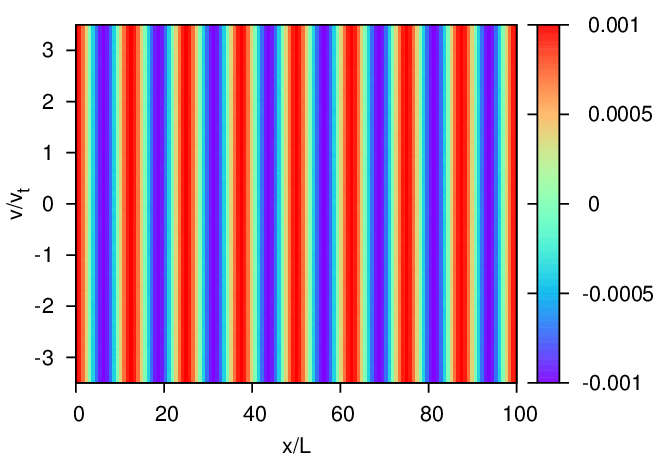
\includegraphics{/home/yj/project_new/read_gfile/fig85/map.eps}%
\lthtmlpictureZ
\lthtmlcheckvsize\clearpage}

{\newpage\clearpage
\lthtmlpictureA{tex2html_wrap14945}%
\includegraphics{/home/yj/project_new/read_gfile/fig60/eigendisplacement001_real.eps}%
\lthtmlpictureZ
\lthtmlcheckvsize\clearpage}

{\newpage\clearpage
\lthtmlpictureA{tex2html_wrap14946}%
\includegraphics{/home/yj/project_new/read_gfile/fig60/eigendisplacement001_imag.eps}%
\lthtmlpictureZ
\lthtmlcheckvsize\clearpage}

{\newpage\clearpage
\lthtmlpictureA{tex2html_wrap14947}%
\includegraphics{/home/yj/project_new/read_gfile/fig60/eigendisplacement001_abs.eps}%
\lthtmlpictureZ
\lthtmlcheckvsize\clearpage}

{\newpage\clearpage
\lthtmlpictureA{tex2html_wrap14967}%
\includegraphics{/home/yj/project_new/read_gfile/fig61/continua.eps}%
\lthtmlpictureZ
\lthtmlcheckvsize\clearpage}

{\newpage\clearpage
\lthtmlinlinemathA{tex2html_wrap_inline14969}%
$ p_0 (0) = 1.5 \times 10^4 \ensuremath{\operatorname{Pa}}$%
\lthtmlinlinemathZ
\lthtmlcheckvsize\clearpage}

{\newpage\clearpage
\lthtmlpictureA{tex2html_wrap14991}%
\includegraphics{/home/yj/project_new/read_gfile/fig58/dis_real.eps}%
\lthtmlpictureZ
\lthtmlcheckvsize\clearpage}

{\newpage\clearpage
\lthtmlpictureA{tex2html_wrap14992}%
\includegraphics{/home/yj/project_new/read_gfile/fig58/dis_imag.eps}%
\lthtmlpictureZ
\lthtmlcheckvsize\clearpage}

{\newpage\clearpage
\lthtmlpictureA{tex2html_wrap14993}%
\includegraphics{/home/yj/project_new/read_gfile/fig58/dis_abs.eps}%
\lthtmlpictureZ
\lthtmlcheckvsize\clearpage}

{\newpage\clearpage
\lthtmlpictureA{tex2html_wrap15013}%
\includegraphics{/home/yj/project_new/read_gfile/fig58/continua.eps}%
\lthtmlpictureZ
\lthtmlcheckvsize\clearpage}

\stepcounter{section}
\stepcounter{subsection}
{\newpage\clearpage
\lthtmlinlinemathA{tex2html_wrap_inline15017}%
$ \theta = \ensuremath{\operatorname{const}}$%
\lthtmlinlinemathZ
\lthtmlcheckvsize\clearpage}

{\newpage\clearpage
\lthtmlinlinemathA{tex2html_wrap_inline15019}%
$ \ensuremath{\operatorname{dRsep}}$%
\lthtmlinlinemathZ
\lthtmlcheckvsize\clearpage}

{\newpage\clearpage
\lthtmlpictureA{tex2html_wrap15025}%
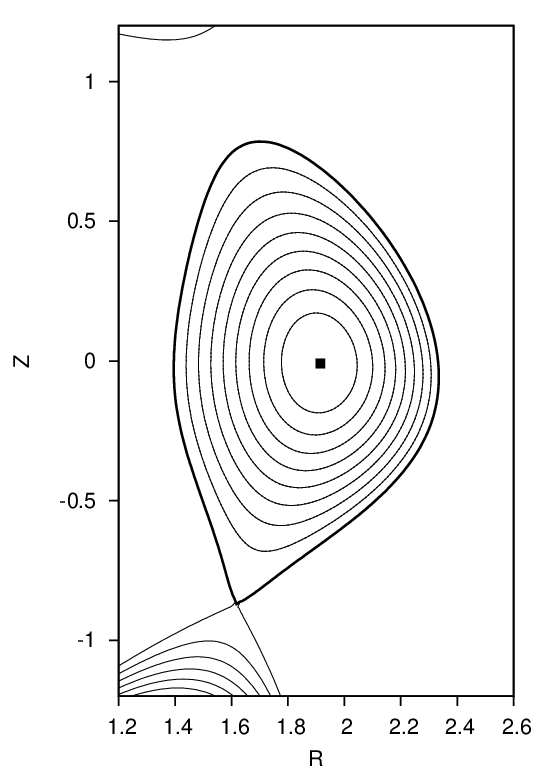
\includegraphics{/home/yj/project_new/read_gfile/fig75/contour.eps}%
\lthtmlpictureZ
\lthtmlcheckvsize\clearpage}

{\newpage\clearpage
\lthtmlpictureA{tex2html_wrap15026}%
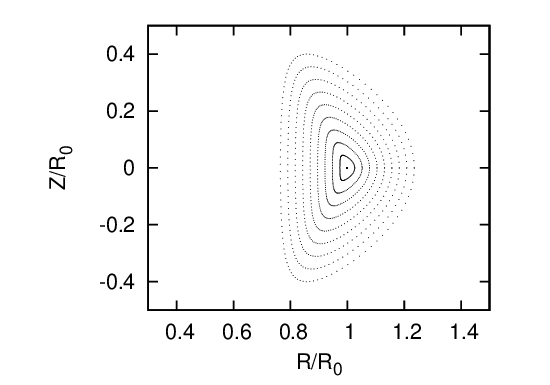
\includegraphics{/home/yj/project_new/read_gfile/fig40/plt.eps}%
\lthtmlpictureZ
\lthtmlcheckvsize\clearpage}

{\newpage\clearpage
\lthtmlpictureA{tex2html_wrap15030}%
\includegraphics{/home/yj/project_new/read_gfile/fig37/pressure_q.eps}%
\lthtmlpictureZ
\lthtmlcheckvsize\clearpage}

{\newpage\clearpage
\lthtmlpictureA{tex2html_wrap15031}%
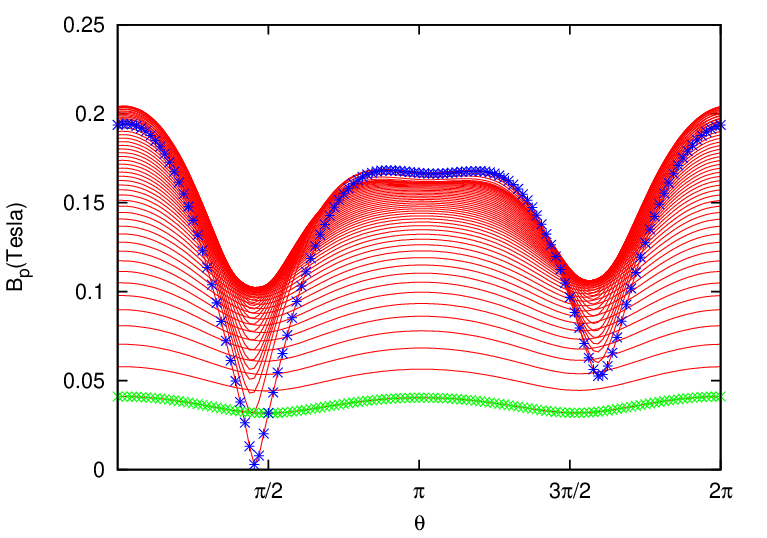
\includegraphics{/home/yj/project_new/read_gfile/fig37/p3.eps}%
\lthtmlpictureZ
\lthtmlcheckvsize\clearpage}

{\newpage\clearpage
\lthtmlpictureA{tex2html_wrap15032}%
\includegraphics{/home/yj/project_new/read_gfile/fig37/fpsi.eps}%
\lthtmlpictureZ
\lthtmlcheckvsize\clearpage}

{\newpage\clearpage
\lthtmlinlinemathA{tex2html_wrap_inline15036}%
$ \rho_0 = m_i n_i$%
\lthtmlinlinemathZ
\lthtmlcheckvsize\clearpage}

{\newpage\clearpage
\lthtmlinlinemathA{tex2html_wrap_inline15038}%
$ m_i$%
\lthtmlinlinemathZ
\lthtmlcheckvsize\clearpage}

{\newpage\clearpage
\lthtmlinlinemathA{tex2html_wrap_inline15040}%
$ n_i$%
\lthtmlinlinemathZ
\lthtmlcheckvsize\clearpage}

{\newpage\clearpage
\lthtmlinlinemathA{tex2html_wrap_inline15042}%
$ n_e$%
\lthtmlinlinemathZ
\lthtmlcheckvsize\clearpage}

{\newpage\clearpage
\lthtmlinlinemathA{tex2html_wrap_inline15044}%
$ n_i = n_e$%
\lthtmlinlinemathZ
\lthtmlcheckvsize\clearpage}

{\newpage\clearpage
\lthtmlpictureA{tex2html_wrap15048}%
\includegraphics{/home/yj/project_new/read_gfile/fig49/normal.eps}%
\lthtmlpictureZ
\lthtmlcheckvsize\clearpage}

{\newpage\clearpage
\lthtmlpictureA{tex2html_wrap15049}%
\includegraphics{/home/yj/project_new/read_gfile/fig49/geodesic.eps}%
\lthtmlpictureZ
\lthtmlcheckvsize\clearpage}

{\newpage\clearpage
\lthtmlpictureA{tex2html_wrap15057}%
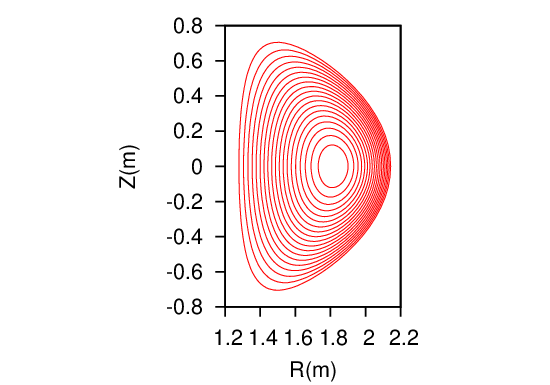
\includegraphics{/home/yj/project_new/read_gfile/fig33/tmp2.eps}%
\lthtmlpictureZ
\lthtmlcheckvsize\clearpage}

{\newpage\clearpage
\lthtmlpictureA{tex2html_wrap15069}%
\includegraphics{/home/yj/project_new/read_gfile/fig49/sigma.eps}%
\lthtmlpictureZ
\lthtmlcheckvsize\clearpage}

\stepcounter{subsection}
{\newpage\clearpage
\lthtmlinlinemathA{tex2html_wrap_inline15102}%
$ (1, 2)$%
\lthtmlinlinemathZ
\lthtmlcheckvsize\clearpage}

{\newpage\clearpage
\lthtmlpictureA{tex2html_wrap15118}%
\includegraphics{/home/yj/project_new/read_gfile/fig50/kHz.eps}%
\lthtmlpictureZ
\lthtmlcheckvsize\clearpage}

{\newpage\clearpage
\lthtmlpictureA{tex2html_wrap15138}%
\includegraphics{/home/yj/project_new/read_gfile/fig51/full_continua.eps}%
\lthtmlpictureZ
\lthtmlcheckvsize\clearpage}

{\newpage\clearpage
\lthtmlpictureA{tex2html_wrap15139}%
\includegraphics{/home/yj/project_new/read_gfile/fig51/slow_sound.eps}%
\lthtmlpictureZ
\lthtmlcheckvsize\clearpage}

{\newpage\clearpage
\lthtmlpictureA{tex2html_wrap15140}%
\includegraphics{/home/yj/project_new/read_gfile/fig51/zero_beta_continua.eps}%
\lthtmlpictureZ
\lthtmlcheckvsize\clearpage}

{\newpage\clearpage
\lthtmlpictureA{tex2html_wrap15158}%
\includegraphics{/home/yj/project_new/read_gfile/compare3/p.eps}%
\lthtmlpictureZ
\lthtmlcheckvsize\clearpage}

{\newpage\clearpage
\lthtmlinlinemathA{tex2html_wrap_inline15164}%
$ n (q_{\ensuremath{\operatorname{edge}}} - q_{\ensuremath{\operatorname{axis}}})$%
\lthtmlinlinemathZ
\lthtmlcheckvsize\clearpage}

{\newpage\clearpage
\lthtmlpictureA{tex2html_wrap15178}%
\includegraphics{/home/yj/project_new/read_gfile/fig52/tmp.eps}%
\lthtmlpictureZ
\lthtmlcheckvsize\clearpage}

{\newpage\clearpage
\lthtmlinlinemathA{tex2html_wrap_indisplay15182}%
$\displaystyle \langle W \rangle_{m' m} = \frac{1}{2 \pi} \int_0^{2 \pi} W   e^{i (m + m') \theta} d \theta,$%
\lthtmlindisplaymathZ
\lthtmlcheckvsize\clearpage}

{\newpage\clearpage
\lthtmlinlinemathA{tex2html_wrap_inline15184}%
$ [- 10, 15]$%
\lthtmlinlinemathZ
\lthtmlcheckvsize\clearpage}

\stepcounter{subsection}
{\newpage\clearpage
\lthtmlinlinemathA{tex2html_wrap_inline15191}%
$ [c_1 \ln | \psi - \psi_s | + c_2]$%
\lthtmlinlinemathZ
\lthtmlcheckvsize\clearpage}

{\newpage\clearpage
\lthtmlinlinemathA{tex2html_wrap_inline15193}%
$ \psi_s$%
\lthtmlinlinemathZ
\lthtmlcheckvsize\clearpage}

{\newpage\clearpage
\lthtmlinlinemathA{tex2html_wrap_inline15195}%
$ c_2$%
\lthtmlinlinemathZ
\lthtmlcheckvsize\clearpage}

{\newpage\clearpage
\lthtmlpictureA{tex2html_wrap15217}%
\includegraphics{/home/yj/project_new/read_gfile/fig53/dis_real.eps}%
\lthtmlpictureZ
\lthtmlcheckvsize\clearpage}

{\newpage\clearpage
\lthtmlpictureA{tex2html_wrap15218}%
\includegraphics{/home/yj/project_new/read_gfile/fig53/dis_imag.eps}%
\lthtmlpictureZ
\lthtmlcheckvsize\clearpage}

{\newpage\clearpage
\lthtmlpictureA{tex2html_wrap15219}%
\includegraphics{/home/yj/project_new/read_gfile/fig53/dis_abs.eps}%
\lthtmlpictureZ
\lthtmlcheckvsize\clearpage}

{\newpage\clearpage
\lthtmlpictureA{tex2html_wrap15239}%
\includegraphics{/home/yj/project_new/read_gfile/fig53/continua.eps}%
\lthtmlpictureZ
\lthtmlcheckvsize\clearpage}

{\newpage\clearpage
\lthtmlpictureA{tex2html_wrap15261}%
\includegraphics{/home/yj/project_new/read_gfile/fig57/dis_real.eps}%
\lthtmlpictureZ
\lthtmlcheckvsize\clearpage}

{\newpage\clearpage
\lthtmlpictureA{tex2html_wrap15262}%
\includegraphics{/home/yj/project_new/read_gfile/fig57/dis_imag.eps}%
\lthtmlpictureZ
\lthtmlcheckvsize\clearpage}

{\newpage\clearpage
\lthtmlpictureA{tex2html_wrap15263}%
\includegraphics{/home/yj/project_new/read_gfile/fig57/dis_abs.eps}%
\lthtmlpictureZ
\lthtmlcheckvsize\clearpage}

{\newpage\clearpage
\lthtmlpictureA{tex2html_wrap15283}%
\includegraphics{/home/yj/project_new/read_gfile/fig57/continua.eps}%
\lthtmlpictureZ
\lthtmlcheckvsize\clearpage}

{\newpage\clearpage
\lthtmlpictureA{tex2html_wrap15309}%
\includegraphics{/home/yj/project_new/read_gfile/fig55/dis_real.eps}%
\lthtmlpictureZ
\lthtmlcheckvsize\clearpage}

{\newpage\clearpage
\lthtmlpictureA{tex2html_wrap15310}%
\includegraphics{/home/yj/project_new/read_gfile/fig55/dis_imag.eps}%
\lthtmlpictureZ
\lthtmlcheckvsize\clearpage}

{\newpage\clearpage
\lthtmlpictureA{tex2html_wrap15311}%
\includegraphics{/home/yj/project_new/read_gfile/fig55/dis_abs.eps}%
\lthtmlpictureZ
\lthtmlcheckvsize\clearpage}

{\newpage\clearpage
\lthtmlpictureA{tex2html_wrap15319}%
\includegraphics{/home/yj/project_new/read_gfile/fig55/continua.eps}%
\lthtmlpictureZ
\lthtmlcheckvsize\clearpage}

{\newpage\clearpage
\lthtmlpictureA{tex2html_wrap15339}%
\includegraphics{/home/yj/project_new/read_gfile/fig54/dis_real.eps}%
\lthtmlpictureZ
\lthtmlcheckvsize\clearpage}

{\newpage\clearpage
\lthtmlpictureA{tex2html_wrap15340}%
\includegraphics{/home/yj/project_new/read_gfile/fig54/dis_imag.eps}%
\lthtmlpictureZ
\lthtmlcheckvsize\clearpage}

{\newpage\clearpage
\lthtmlpictureA{tex2html_wrap15341}%
\includegraphics{/home/yj/project_new/read_gfile/fig54/dis_abs.eps}%
\lthtmlpictureZ
\lthtmlcheckvsize\clearpage}

{\newpage\clearpage
\lthtmlpictureA{tex2html_wrap15349}%
\includegraphics{/home/yj/project_new/read_gfile/fig54/continua.eps}%
\lthtmlpictureZ
\lthtmlcheckvsize\clearpage}

{\newpage\clearpage
\lthtmlpictureA{tex2html_wrap15375}%
\includegraphics{/home/yj/project_new/read_gfile/fig48/dis_real.eps}%
\lthtmlpictureZ
\lthtmlcheckvsize\clearpage}

{\newpage\clearpage
\lthtmlpictureA{tex2html_wrap15376}%
\includegraphics{/home/yj/project_new/read_gfile/fig48/dis_imag.eps}%
\lthtmlpictureZ
\lthtmlcheckvsize\clearpage}

{\newpage\clearpage
\lthtmlpictureA{tex2html_wrap15377}%
\includegraphics{/home/yj/project_new/read_gfile/fig48/dis_abs.eps}%
\lthtmlpictureZ
\lthtmlcheckvsize\clearpage}

{\newpage\clearpage
\lthtmlpictureA{tex2html_wrap15381}%
\includegraphics{/home/yj/project_new/read_gfile/fig48/tmp.eps}%
\lthtmlpictureZ
\lthtmlcheckvsize\clearpage}

\stepcounter{subsection}
{\newpage\clearpage
\lthtmlinlinemathA{tex2html_wrap_inline15384}%
$ (\psi, \theta, \phi)$%
\lthtmlinlinemathZ
\lthtmlcheckvsize\clearpage}

{\newpage\clearpage
\lthtmlinlinemathA{tex2html_wrap_inline15388}%
$ \ensuremath{\boldsymbol{\kappa}}=\mathbf{b} \cdot \nabla \mathbf{b}$%
\lthtmlinlinemathZ
\lthtmlcheckvsize\clearpage}

{\newpage\clearpage
\lthtmlinlinemathA{tex2html_wrap_indisplay15391}%
$\displaystyle \ensuremath{\boldsymbol{\kappa}}$%
\lthtmlindisplaymathZ
\lthtmlcheckvsize\clearpage}

{\newpage\clearpage
\lthtmlinlinemathA{tex2html_wrap_indisplay15395}%
$\displaystyle \frac{1}{B_0} \mathbf{B}_0 \cdot \nabla
\frac{\mathbf{B}_0}{B_0}$%
\lthtmlindisplaymathZ
\lthtmlcheckvsize\clearpage}

{\newpage\clearpage
\lthtmlinlinemathA{tex2html_wrap_indisplay15399}%
$\displaystyle \frac{1}{B_0} (\nabla \Psi \times \nabla \phi + g \nabla \phi) \cdot
\nabla \frac{\mathbf{B}_0}{B_0}$%
\lthtmlindisplaymathZ
\lthtmlcheckvsize\clearpage}

{\newpage\clearpage
\lthtmlinlinemathA{tex2html_wrap_indisplay15408}%
$\displaystyle \frac{1}{B_0} (\Psi' \triangledown \psi \times
\triangledown \phi + g \triangledown \phi) \cdot \nabla
\frac{\mathbf{B}_0}{B_0}$%
\lthtmlindisplaymathZ
\lthtmlcheckvsize\clearpage}

{\newpage\clearpage
\lthtmlinlinemathA{tex2html_wrap_indisplay15412}%
$\displaystyle \frac{\Psi'}{B_0} (\triangledown \psi \times \triangledown \phi)
\cdot \nabla \frac{\mathbf{B}_0}{B_0} + \frac{g}{B_0} \triangledown \phi
\cdot \nabla \frac{\mathbf{B}_0}{B_0}$%
\lthtmlindisplaymathZ
\lthtmlcheckvsize\clearpage}

{\newpage\clearpage
\lthtmlinlinemathA{tex2html_wrap_indisplay15416}%
$\displaystyle - \frac{\Psi'}{B_0} \mathcal{J}^{- 1} \frac{\partial}{\partial
\theta} \left( \frac{\mathbf{B}_0}{B_0} \right) + \frac{g}{B_0}
\frac{1}{R^2}  \frac{\partial}{\partial \phi} \left(
\frac{\mathbf{B}_0}{B_0} \right)$%
\lthtmlindisplaymathZ
\lthtmlcheckvsize\clearpage}

{\newpage\clearpage
\lthtmlinlinemathA{tex2html_wrap_indisplay15420}%
$\displaystyle - \frac{\Psi'}{B_0} \mathcal{J}^{- 1} \frac{\partial}{\partial
\theta} \left( \frac{\Psi' \triangledown \psi \times \triangledown \phi + g
\triangledown \phi}{B_0} \right) + \frac{g}{B_0}  \frac{1}{R^2}
\frac{\partial}{\partial \phi} \left( \frac{\Psi' \triangledown \psi \times
\triangledown \phi + g \triangledown \phi}{B_0} \right)$%
\lthtmlindisplaymathZ
\lthtmlcheckvsize\clearpage}

{\newpage\clearpage
\lthtmlinlinemathA{tex2html_wrap_indisplay15424}%
$\displaystyle - \frac{\Psi'^2}{B_0} \mathcal{J}^{- 1} \frac{\partial}{\partial
\theta} \left( \frac{\triangledown \psi \times \triangledown \phi}{B_0}
\right) - \frac{g \Psi'}{B_0} \mathcal{J}^{- 1} \frac{\partial}{\partial
\theta} \left( \frac{\triangledown \phi}{B_0} \right) + \frac{g \Psi'}{B_0^2
R^2}  \frac{\partial}{\partial \phi} (\triangledown \psi \times
\triangledown \phi) - \frac{g^2}{B_0^2}  \frac{1}{R^3}  \hat{\mathbf{R}}$%
\lthtmlindisplaymathZ
\lthtmlcheckvsize\clearpage}

{\newpage\clearpage
\lthtmlinlinemathA{tex2html_wrap_inline15426}%
$ \nabla \psi = - \frac{R}{\mathcal{J}} (Z_{\theta} \hat{\mathbf{R}} -
R_{\theta} \hat{\mathbf{Z}})$%
\lthtmlinlinemathZ
\lthtmlcheckvsize\clearpage}

{\newpage\clearpage
\lthtmlinlinemathA{tex2html_wrap_inline15428}%
$ \nabla \psi \times \triangledown
\phi = - \frac{1}{\mathcal{J}} (Z_{\theta} \hat{\mathbf{Z}} + R_{\theta}
\hat{\mathbf{R}})$%
\lthtmlinlinemathZ
\lthtmlcheckvsize\clearpage}

{\newpage\clearpage
\lthtmlinlinemathA{tex2html_wrap_indisplay15431}%
$\displaystyle \frac{\partial}{\partial \theta} \left( \frac{\triangledown \psi \times
\triangledown \phi}{B_0} \right)$%
\lthtmlindisplaymathZ
\lthtmlcheckvsize\clearpage}

{\newpage\clearpage
\lthtmlinlinemathA{tex2html_wrap_indisplay15435}%
$\displaystyle - (Z_{\theta} \hat{\mathbf{Z}} +
R_{\theta} \hat{\mathbf{R}}) \frac{\partial}{\partial \theta} \left(
\frac{\mathcal{J}^{- 1}}{B_0} \right) - \frac{\mathcal{J}^{- 1}}{B_0}
(Z_{\theta \theta} \hat{\mathbf{Z}} + R_{\theta \theta} \hat{\mathbf{R}})$%
\lthtmlindisplaymathZ
\lthtmlcheckvsize\clearpage}

{\newpage\clearpage
\lthtmlinlinemathA{tex2html_wrap_indisplay15439}%
$\displaystyle - \left[ \frac{\partial}{\partial \theta} \left( \frac{\mathcal{J}^{-
1}}{B_0} \right) R_{\theta} + \frac{\mathcal{J}^{- 1}}{B_0} R_{\theta
\theta} \right] \hat{\mathbf{R}} - \left[ \frac{\partial}{\partial \theta}
\left( \frac{\mathcal{J}^{- 1}}{B_0} \right) Z_{\theta} +
\frac{\mathcal{J}^{- 1}}{B_0} Z_{\theta \theta} \right] \hat{\mathbf{Z}},$%
\lthtmlindisplaymathZ
\lthtmlcheckvsize\clearpage}

{\newpage\clearpage
\lthtmlinlinemathA{tex2html_wrap_indisplay15441}%
$\displaystyle \frac{\partial}{\partial \theta} \left( \frac{\triangledown \phi}{B_0}   \right) = \frac{\partial}{\partial \theta} \left( \frac{1}{R B_0} \right)   \hat{\ensuremath{\boldsymbol{\phi}}},$%
\lthtmlindisplaymathZ
\lthtmlcheckvsize\clearpage}

{\newpage\clearpage
\lthtmlinlinemathA{tex2html_wrap_indisplay15443}%
$\displaystyle \frac{\partial}{\partial \phi} (\triangledown \psi \times \triangledown   \phi) = - \frac{1}{\mathcal{J}} R_{\theta} \hat{\ensuremath{\boldsymbol{\phi}}} .$%
\lthtmlindisplaymathZ
\lthtmlcheckvsize\clearpage}

{\newpage\clearpage
\lthtmlinlinemathA{tex2html_wrap_inline15445}%
$ \ensuremath{\boldsymbol{\kappa}}$%
\lthtmlinlinemathZ
\lthtmlcheckvsize\clearpage}

{\newpage\clearpage
\lthtmlinlinemathA{tex2html_wrap_indisplay15452}%
$\displaystyle \frac{\Psi'^2}{B_0} \mathcal{J}^{- 1} \left\{ \left[
\frac{\partial}{\partial \theta} \left( \frac{\mathcal{J}^{- 1}}{B_0}
\right) R_{\theta} + \frac{\mathcal{J}^{- 1}}{B_0} R_{\theta \theta} \right]
\hat{\mathbf{R}} + \left[ \frac{\partial}{\partial \theta} \left(
\frac{\mathcal{J}^{- 1}}{B_0} \right) Z_{\theta} + \frac{\mathcal{J}^{-
1}}{B_0} Z_{\theta \theta} \right] \hat{\mathbf{Z}} \right\}$%
\lthtmlindisplaymathZ
\lthtmlcheckvsize\clearpage}

{\newpage\clearpage
\lthtmlinlinemathA{tex2html_wrap_indisplay15454}%
$\displaystyle - \frac{g \Psi'}{B_0} \mathcal{J}^{- 1} \frac{\partial}{\partial
\theta} \left( \frac{1}{R B_0} \right) \hat{\ensuremath{\boldsymbol{\phi}}} - \frac{g
\Psi'}{B_0^2 R^2}  \frac{1}{\mathcal{J}} R_{\theta} \hat{\ensuremath{\boldsymbol{\phi}}} -
\frac{g^2}{B_0^2}  \frac{1}{R^3}  \hat{\mathbf{R}}$%
\lthtmlindisplaymathZ
\lthtmlcheckvsize\clearpage}

\stepcounter{subsubsection}
{\newpage\clearpage
\lthtmlinlinemathA{tex2html_wrap_inline15461}%
$ \kappa_{\psi} =\ensuremath{\boldsymbol{\kappa}}
\cdot \nabla \Psi$%
\lthtmlinlinemathZ
\lthtmlcheckvsize\clearpage}

{\newpage\clearpage
\lthtmlinlinemathA{tex2html_wrap_indisplay15466}%
$\displaystyle \kappa_{\psi}$%
\lthtmlindisplaymathZ
\lthtmlcheckvsize\clearpage}

{\newpage\clearpage
\lthtmlinlinemathA{tex2html_wrap_indisplay15470}%
$\displaystyle - \frac{\Psi'^3}{B_0} \mathcal{J}^{- 1}
\frac{\partial}{\partial \theta} \left( \frac{\triangledown \psi \times
\triangledown \phi}{B_0} \right) \cdot \nabla \psi + 0 + 0 - \frac{\Psi'
g^2}{B_0^2}  \frac{1}{R^3}  \hat{\mathbf{R}} \cdot \nabla \psi$%
\lthtmlindisplaymathZ
\lthtmlcheckvsize\clearpage}

{\newpage\clearpage
\lthtmlinlinemathA{tex2html_wrap_indisplay15474}%
$\displaystyle - \frac{\Psi'^3}{B_0} \mathcal{J}^{- 1} \left\{ \left[
\frac{\partial}{\partial \theta} \left( \frac{\mathcal{J}^{- 1}}{B_0}
\right) R_{\theta} + \frac{\mathcal{J}^{- 1}}{B_0} R_{\theta \theta} \right]
\hat{\mathbf{R}} + \left[ \frac{\partial}{\partial \theta} \left(
\frac{\mathcal{J}^{- 1}}{B_0} \right) Z_{\theta} + \frac{\mathcal{J}^{-
1}}{B_0} Z_{\theta \theta} \right] \hat{\mathbf{Z}} \right\} \cdot \left[
\frac{R}{\mathcal{J}} (Z_{\theta} \hat{\mathbf{R}} - R_{\theta}
\hat{\mathbf{Z}}) \right] - \frac{\Psi' g^2}{B_0^2}  \frac{1}{R^3}
\hat{\mathbf{R}} \cdot \left[ - \frac{R}{\mathcal{J}} (Z_{\theta}
\hat{\mathbf{R}} - R_{\theta} \hat{\mathbf{Z}}) \right]$%
\lthtmlindisplaymathZ
\lthtmlcheckvsize\clearpage}

{\newpage\clearpage
\lthtmlinlinemathA{tex2html_wrap_indisplay15478}%
$\displaystyle - \frac{\Psi'^3}{B_0} \mathcal{J}^{- 1} \frac{R}{\mathcal{J}} \left\{
\left[ \frac{\partial}{\partial \theta} \left( \frac{\mathcal{J}^{- 1}}{B_0}
\right) R_{\theta} + \frac{\mathcal{J}^{- 1}}{B_0} R_{\theta \theta} \right]
Z_{\theta} - \left[ \frac{\partial}{\partial \theta} \left(
\frac{\mathcal{J}^{- 1}}{B_0} \right) Z_{\theta} + \frac{\mathcal{J}^{-
1}}{B_0} Z_{\theta \theta} \right] R_{\theta} \right\} + \frac{\Psi'
g^2}{B_0^2}  \frac{1}{R^2}  \frac{1}{\mathcal{J}} Z_{\theta}$%
\lthtmlindisplaymathZ
\lthtmlcheckvsize\clearpage}

{\newpage\clearpage
\lthtmlinlinemathA{tex2html_wrap_indisplay15482}%
$\displaystyle - \frac{\Psi'^3}{B_0} \mathcal{J}^{- 1} \frac{R}{\mathcal{J}}
\frac{\mathcal{J}^{- 1}}{B_0} (R_{\theta \theta} Z_{\theta} - R_{\theta}
Z_{\theta \theta}) + \frac{\Psi' g^2}{B_0^2}  \frac{1}{R^2}
\frac{1}{\mathcal{J}} Z_{\theta}$%
\lthtmlindisplaymathZ
\lthtmlcheckvsize\clearpage}

{\newpage\clearpage
\lthtmlinlinemathA{tex2html_wrap_indisplay15486}%
$\displaystyle - \Psi'^3 R \frac{\mathcal{J}^{- 3}}{B_0^2} (R_{\theta \theta}
Z_{\theta} - R_{\theta} Z_{\theta \theta}) + \frac{\Psi' g^2}{B_0^2}
\frac{1}{R^2}  \frac{1}{\mathcal{J}} Z_{\theta}$%
\lthtmlindisplaymathZ
\lthtmlcheckvsize\clearpage}

{\newpage\clearpage
\lthtmlinlinemathA{tex2html_wrap_indisplay15490}%
$\displaystyle - \Psi'^3 R \frac{\mathcal{J}^{- 3}}{B_0^2} Z_{\theta}^2
\frac{\partial}{\partial \theta} \left( \frac{R_{\theta}}{Z_{\theta}}
\right) + \frac{\Psi' g^2}{B_0^2}  \frac{1}{R^2}  \frac{1}{\mathcal{J}}
Z_{\theta} .$%
\lthtmlindisplaymathZ
\lthtmlcheckvsize\clearpage}

{\newpage\clearpage
\lthtmlinlinemathA{tex2html_wrap_inline15494}%
$ Z_{\theta}$%
\lthtmlinlinemathZ
\lthtmlcheckvsize\clearpage}

{\newpage\clearpage
\lthtmlpictureA{tex2html_wrap15506}%
\includegraphics{/home/yj/project_new/read_gfile/fig30/tmp2.eps}%
\lthtmlpictureZ
\lthtmlcheckvsize\clearpage}

{\newpage\clearpage
\lthtmlpictureA{tex2html_wrap15507}%
\includegraphics{/home/yj/project_new/read_gfile/fig30/tmp3.eps}%
\lthtmlpictureZ
\lthtmlcheckvsize\clearpage}

\stepcounter{subsubsection}
{\newpage\clearpage
\lthtmlinlinemathA{tex2html_wrap_indisplay15516}%
$\displaystyle \kappa_s \equiv \ensuremath{\boldsymbol{\kappa}} \cdot \frac{\mathbf{B}_0   \times \nabla \Psi}{B_0^2} .$%
\lthtmlindisplaymathZ
\lthtmlcheckvsize\clearpage}

{\newpage\clearpage
\lthtmlinlinemathA{tex2html_wrap_indisplay15519}%
$\displaystyle \mathbf{B}_0 \times \nabla \Psi$%
\lthtmlindisplaymathZ
\lthtmlcheckvsize\clearpage}

{\newpage\clearpage
\lthtmlinlinemathA{tex2html_wrap_indisplay15523}%
$\displaystyle [\nabla \Psi \times \nabla \phi + g
\nabla \phi] \times \nabla \Psi$%
\lthtmlindisplaymathZ
\lthtmlcheckvsize\clearpage}

{\newpage\clearpage
\lthtmlinlinemathA{tex2html_wrap_indisplay15527}%
$\displaystyle \Psi'^2 | \nabla \psi |^2 \nabla \phi - g \Psi' \nabla \psi \times
\nabla \phi$%
\lthtmlindisplaymathZ
\lthtmlcheckvsize\clearpage}

{\newpage\clearpage
\lthtmlinlinemathA{tex2html_wrap_indisplay15531}%
$\displaystyle \Psi'^2 | \nabla \psi |^2 \frac{1}{R} \hat{\ensuremath{\boldsymbol{\phi}}} + \frac{g
\Psi'}{\mathcal{J}} Z_{\theta} \hat{\mathbf{Z}} + \frac{g
\Psi'}{\mathcal{J}} R_{\theta} \hat{\mathbf{R}}$%
\lthtmlindisplaymathZ
\lthtmlcheckvsize\clearpage}

{\newpage\clearpage
\lthtmlinlinemathA{tex2html_wrap_indisplay15534}%
$\displaystyle \frac{\partial}{\partial \theta} \left( \frac{\triangledown \psi \times
\triangledown \phi}{B_0} \right) \cdot \frac{\mathbf{B}_0 \times \nabla
\Psi}{B_0^2}$%
\lthtmlindisplaymathZ
\lthtmlcheckvsize\clearpage}

{\newpage\clearpage
\lthtmlinlinemathA{tex2html_wrap_indisplay15538}%
$\displaystyle \left\{ - \left[ \frac{\partial}{\partial \theta} \left(
\frac{\mathcal{J}^{- 1}}{B_0} \right) R_{\theta} + \frac{\mathcal{J}^{-
1}}{B_0} R_{\theta \theta} \right] \hat{\mathbf{R}} - \left[
\frac{\partial}{\partial \theta} \left( \frac{\mathcal{J}^{- 1}}{B_0}
\right) Z_{\theta} + \frac{\mathcal{J}^{- 1}}{B_0} Z_{\theta \theta} \right]
\hat{\mathbf{Z}} \right\} \cdot \frac{g \Psi'}{B_0^2 \mathcal{J}}
(Z_{\theta} \hat{\mathbf{Z}} + R_{\theta} \hat{\mathbf{R}})$%
\lthtmlindisplaymathZ
\lthtmlcheckvsize\clearpage}

{\newpage\clearpage
\lthtmlinlinemathA{tex2html_wrap_indisplay15542}%
$\displaystyle - \frac{g \Psi'}{B_0^2 \mathcal{J}} \left\{ \left[
\frac{\partial}{\partial \theta} \left( \frac{\mathcal{J}^{- 1}}{B_0}
\right) Z_{\theta} + \frac{\mathcal{J}^{- 1}}{B_0} Z_{\theta \theta} \right]
Z_{\theta} + \left[ \frac{\partial}{\partial \theta} \left(
\frac{\mathcal{J}^{- 1}}{B_0} \right) R_{\theta} + \frac{\mathcal{J}^{-
1}}{B_0} R_{\theta \theta} \right] R_{\theta} \right\}$%
\lthtmlindisplaymathZ
\lthtmlcheckvsize\clearpage}

{\newpage\clearpage
\lthtmlinlinemathA{tex2html_wrap_indisplay15545}%
$\displaystyle \frac{\partial}{\partial \theta} \left( \frac{\triangledown \phi}{B_0}
\right) \cdot \frac{\mathbf{B}_0 \times \nabla \Psi}{B_0^2}$%
\lthtmlindisplaymathZ
\lthtmlcheckvsize\clearpage}

{\newpage\clearpage
\lthtmlinlinemathA{tex2html_wrap_indisplay15549}%
$\displaystyle \frac{\partial}{\partial \theta} \left( \frac{1}{R B_0} \right)
\frac{\Psi'^2 | \nabla \psi |^2}{B_0^2 R} .$%
\lthtmlindisplaymathZ
\lthtmlcheckvsize\clearpage}

{\newpage\clearpage
\lthtmlinlinemathA{tex2html_wrap_indisplay15552}%
$\displaystyle \frac{\partial}{\partial \phi} (\triangledown \psi \times \triangledown
\phi) \cdot \frac{\mathbf{B}_0 \times \nabla \Psi}{B_0^2}$%
\lthtmlindisplaymathZ
\lthtmlcheckvsize\clearpage}

{\newpage\clearpage
\lthtmlinlinemathA{tex2html_wrap_indisplay15556}%
$\displaystyle -
\frac{1}{\mathcal{J}} R_{\theta} \frac{\Psi'^2 | \nabla \psi |^2}{B_0^2 R} .$%
\lthtmlindisplaymathZ
\lthtmlcheckvsize\clearpage}

{\newpage\clearpage
\lthtmlinlinemathA{tex2html_wrap_indisplay15559}%
$\displaystyle \kappa_s$%
\lthtmlindisplaymathZ
\lthtmlcheckvsize\clearpage}

{\newpage\clearpage
\lthtmlinlinemathA{tex2html_wrap_indisplay15563}%
$\displaystyle - \frac{\Psi'^2}{B_0} \mathcal{J}^{- 1} \left( - \frac{g
\Psi'}{B_0^2 \mathcal{J}} \right) \left\{ \left[ \frac{\partial}{\partial
\theta} \left( \frac{\mathcal{J}^{- 1}}{B_0} \right) Z_{\theta} +
\frac{\mathcal{J}^{- 1}}{B_0} Z_{\theta \theta} \right] Z_{\theta} + \left[
\frac{\partial}{\partial \theta} \left( \frac{\mathcal{J}^{- 1}}{B_0}
\right) R_{\theta} + \frac{\mathcal{J}^{- 1}}{B_0} R_{\theta \theta} \right]
R_{\theta} \right\}$%
\lthtmlindisplaymathZ
\lthtmlcheckvsize\clearpage}

{\newpage\clearpage
\lthtmlinlinemathA{tex2html_wrap_indisplay15565}%
$\displaystyle - \frac{g \Psi'}{B_0} \mathcal{J}^{- 1} \frac{\partial}{\partial
\theta} \left( \frac{1}{R B_0} \right) \frac{\Psi'^2 | \nabla \psi
|^2}{B_0^2 R} - \frac{g \Psi'}{B_0^2}  \frac{1}{R^2}  \frac{1}{\mathcal{J}}
R_{\theta} \frac{\Psi'^2 | \nabla \psi |^2}{B_0^2 R} - \frac{g^2}{B_0^2}
\frac{1}{R^3}  \frac{g \Psi'}{B_0^2 \mathcal{J}} R_{\theta}$%
\lthtmlindisplaymathZ
\lthtmlcheckvsize\clearpage}

{\newpage\clearpage
\lthtmlinlinemathA{tex2html_wrap_indisplay15568}%
$\displaystyle \frac{g \Psi'^3}{B_0^3} \mathcal{J}^{- 2} \left[
\frac{\partial}{\partial \theta} \left( \frac{\mathcal{J}^{- 1}}{B_0}
\right) Z_{\theta}^2 + \frac{\mathcal{J}^{- 1}}{B_0} Z_{\theta \theta}
Z_{\theta} + \frac{\partial}{\partial \theta} \left( \frac{\mathcal{J}^{-
1}}{B_0} \right) R_{\theta}^2 + \frac{\mathcal{J}^{- 1}}{B_0} R_{\theta
\theta} R_{\theta} \right]$%
\lthtmlindisplaymathZ
\lthtmlcheckvsize\clearpage}

{\newpage\clearpage
\lthtmlinlinemathA{tex2html_wrap_indisplay15570}%
$\displaystyle = \frac{g \Psi'^3}{B_0^3} \mathcal{J}^{- 2} \left[
\frac{\partial}{\partial \theta} \left( \frac{\mathcal{J}^{- 1}}{B_0}
\right) (Z_{\theta}^2 + R_{\theta}^2) + \frac{\mathcal{J}^{- 1}}{B_0}
(Z_{\theta \theta} Z_{\theta} + R_{\theta \theta} R_{\theta}) \right]$%
\lthtmlindisplaymathZ
\lthtmlcheckvsize\clearpage}

{\newpage\clearpage
\lthtmlinlinemathA{tex2html_wrap_indisplay15572}%
$\displaystyle | \nabla \psi |^2 = \frac{R^2}{\mathcal{J}^2} (Z_{\theta}^2 + R_{\theta}^2),$%
\lthtmlindisplaymathZ
\lthtmlcheckvsize\clearpage}

{\newpage\clearpage
\lthtmlinlinemathA{tex2html_wrap_indisplay15574}%
$\displaystyle \frac{\partial}{\partial \theta} \left( \frac{\mathcal{J}^2 | \nabla \psi   |^2}{R^2} \right) = 2 Z_{\theta} Z_{\theta \theta} + 2 R_{\theta} R_{\theta   \theta}$%
\lthtmlindisplaymathZ
\lthtmlcheckvsize\clearpage}

{\newpage\clearpage
\lthtmlinlinemathA{tex2html_wrap_indisplay15577}%
$\displaystyle \frac{g \Psi'^3}{B_0^3} \mathcal{J}^{- 2} \left[
\frac{\partial}{\partial \theta} \left( \frac{\mathcal{J}^{- 1}}{B_0}
\right) \frac{\mathcal{J}^2 | \nabla \psi |^2}{R^2} + \frac{\mathcal{J}^{-
1}}{B_0}  \frac{1}{2}  \frac{\partial}{\partial \theta} \left(
\frac{\mathcal{J}^2 | \nabla \psi |^2}{R^2} \right) \right]$%
\lthtmlindisplaymathZ
\lthtmlcheckvsize\clearpage}

{\newpage\clearpage
\lthtmlinlinemathA{tex2html_wrap_indisplay15579}%
$\displaystyle = \frac{g \Psi'^3}{B_0^3} \frac{| \nabla \psi |^2}{R^2}
\frac{\partial}{\partial \theta} \left( \frac{\mathcal{J}^{- 1}}{B_0}
\right) + \frac{g \Psi'^3}{B_0^4} \mathcal{J}^{- 3}  \frac{1}{2}
\frac{\partial}{\partial \theta} \left( \frac{\mathcal{J}^2 | \nabla \psi
|^2}{R^2} \right)$%
\lthtmlindisplaymathZ
\lthtmlcheckvsize\clearpage}

{\newpage\clearpage
\lthtmlinlinemathA{tex2html_wrap_indisplay15581}%
$\displaystyle - \frac{g \Psi'^3}{B_0^3} | \nabla \psi |^2 \mathcal{J}^{-   1} \left[ \frac{\partial}{\partial \theta} \left( \frac{1}{R B_0} \right)   \frac{1}{R} + \frac{1}{B_0 R^3} R_{\theta} \right]$%
\lthtmlindisplaymathZ
\lthtmlcheckvsize\clearpage}

{\newpage\clearpage
\lthtmlinlinemathA{tex2html_wrap_indisplay15584}%
$\displaystyle \frac{g \Psi'^3}{B_0^3} \frac{| \nabla \psi |^2}{R^2}
\frac{\partial}{\partial \theta} \left( \frac{\mathcal{J}^{- 1}}{B_0}
\right) - \frac{g \Psi'^3}{B_0^3} | \nabla \psi |^2 \mathcal{J}^{- 1} \left[
\frac{\partial}{\partial \theta} \left( \frac{1}{R B_0} \right) \frac{1}{R}
+ \frac{1}{B_0 R^3} R_{\theta} \right]$%
\lthtmlindisplaymathZ
\lthtmlcheckvsize\clearpage}

{\newpage\clearpage
\lthtmlinlinemathA{tex2html_wrap_indisplay15586}%
$\displaystyle = \frac{g \Psi'^3}{B_0^3} | \nabla \psi |^2 \left[
\frac{\partial}{\partial \theta} \left( \frac{\mathcal{J}^{- 1}}{B_0}
\right) \frac{1}{R^2} -\mathcal{J}^{- 1} \frac{\partial}{\partial \theta}
\left( \frac{1}{R B_0} \right) \frac{1}{R} - \frac{\mathcal{J}^{- 1}}{B_0
R^3} R_{\theta} \right]$%
\lthtmlindisplaymathZ
\lthtmlcheckvsize\clearpage}

{\newpage\clearpage
\lthtmlinlinemathA{tex2html_wrap_indisplay15592}%
$\displaystyle = \frac{g \Psi'^3}{B_0^3} | \nabla \psi |^2 \left[
\frac{\partial}{\partial \theta} \left( \frac{\mathcal{J}^{- 1}}{B_0 R^2}
\right) + \frac{\mathcal{J}^{- 1}}{B_0 R^3} R_{\theta} -\mathcal{J}^{- 1}
\frac{\partial}{\partial \theta} \left( \frac{1}{R B_0} \right) \frac{1}{R}
\right]$%
\lthtmlindisplaymathZ
\lthtmlcheckvsize\clearpage}

{\newpage\clearpage
\lthtmlinlinemathA{tex2html_wrap_indisplay15594}%
$\displaystyle = \frac{g \Psi'^3}{B_0^3} | \nabla \psi |^2 \left\{
\frac{\partial}{\partial \theta} \left( \frac{\mathcal{J}^{- 1}}{B_0 R^2}
\right) -\mathcal{J}^{- 1} \left[ - \frac{1}{B_0 R^3} R_{\theta} +
\frac{\partial}{\partial \theta} \left( \frac{1}{R B_0} \right) \frac{1}{R}
\right] \right\}$%
\lthtmlindisplaymathZ
\lthtmlcheckvsize\clearpage}

{\newpage\clearpage
\lthtmlinlinemathA{tex2html_wrap_indisplay15596}%
$\displaystyle = \frac{g \Psi'^3}{B_0^3} | \nabla \psi |^2 \left\{
\frac{\partial}{\partial \theta} \left( \frac{\mathcal{J}^{- 1}}{B_0 R^2}
\right) -\mathcal{J}^{- 1} \frac{\partial}{\partial \theta} \left(
\frac{1}{R^2 B_0} \right) \right\}$%
\lthtmlindisplaymathZ
\lthtmlcheckvsize\clearpage}

{\newpage\clearpage
\lthtmlinlinemathA{tex2html_wrap_indisplay15598}%
$\displaystyle = \frac{g \Psi'^3}{B_0^3} | \nabla \psi |^2 \left\{ \frac{1}{B_0 R^2}
\frac{\partial}{\partial \theta} (\mathcal{J}^{- 1}) \right\}$%
\lthtmlindisplaymathZ
\lthtmlcheckvsize\clearpage}

{\newpage\clearpage
\lthtmlinlinemathA{tex2html_wrap_indisplay15607}%
$\displaystyle \frac{g \Psi'^3}{B_0^4} \mathcal{J}^{- 3} \frac{1}{2}
\frac{\partial}{\partial \theta} \left( \frac{\mathcal{J}^2 | \nabla \psi
|^2}{R^2} \right) - \frac{\Psi' g^3}{R^3 B_0^4} \mathcal{J}^{- 1} R_{\theta}
+ \frac{g \Psi'^3}{B_0^4 R^2} | \nabla \psi |^2  \frac{\partial}{\partial
\theta} (\mathcal{J}^{- 1})$%
\lthtmlindisplaymathZ
\lthtmlcheckvsize\clearpage}

{\newpage\clearpage
\lthtmlinlinemathA{tex2html_wrap_indisplay15611}%
$\displaystyle \frac{g \Psi'^3}{B_0^4}  \frac{1}{\mathcal{J}^2} \left[  \frac{1}{2}
\mathcal{J}^{- 1} \frac{\partial}{\partial \theta} \left(
\frac{\mathcal{J}^2 | \nabla \psi |^2}{R^2} \right) + \frac{\mathcal{J}^2 |
\nabla \psi |^2 }{R^2}  \frac{\partial}{\partial \theta} (\mathcal{J}^{- 1})
\right] - \frac{\Psi' g^3}{R^3 B_0^4} \mathcal{J}^{- 1} R_{\theta}$%
\lthtmlindisplaymathZ
\lthtmlcheckvsize\clearpage}

{\newpage\clearpage
\lthtmlinlinemathA{tex2html_wrap_indisplay15619}%
$\displaystyle \frac{g \Psi'}{B_0^4}  \frac{1}{\mathcal{J}^2} \left[  \frac{1}{2}
\mathcal{J}^{- 1} \frac{\partial}{\partial \theta} \left(
\frac{\mathcal{J}^2 | \nabla \Psi |^2}{R^2} \right) + \frac{\mathcal{J}^2 |
\nabla \Psi |^2 }{R^2}  \frac{\partial}{\partial \theta} (\mathcal{J}^{- 1})
\right] - \frac{\Psi' g^3}{R^3 B_0^4} \mathcal{J}^{- 1} R_{\theta}$%
\lthtmlindisplaymathZ
\lthtmlcheckvsize\clearpage}

{\newpage\clearpage
\lthtmlinlinemathA{tex2html_wrap_indisplay15623}%
$\displaystyle \frac{g\mathcal{J}^{- 1} \Psi'}{B_0^3}  \left[ \frac{1}{B_0
\mathcal{J}}  \frac{1}{2} \mathcal{J}^{- 1} \frac{\partial}{\partial \theta}
\left( \frac{\mathcal{J}^2 | \nabla \Psi |^2}{R^2} \right) + \frac{1}{B_0
\mathcal{J}} \frac{\mathcal{J}^2 | \nabla \Psi |^2 }{R^2}
\frac{\partial}{\partial \theta} (\mathcal{J}^{- 1}) - \frac{g^2}{R^3 B_0}
R_{\theta} \right]$%
\lthtmlindisplaymathZ
\lthtmlcheckvsize\clearpage}

{\newpage\clearpage
\lthtmlinlinemathA{tex2html_wrap_indisplay15626}%
$\displaystyle \frac{\partial B_0}{\partial \theta}$%
\lthtmlindisplaymathZ
\lthtmlcheckvsize\clearpage}

{\newpage\clearpage
\lthtmlinlinemathA{tex2html_wrap_indisplay15630}%
$\displaystyle \frac{\partial}{\partial \theta}
\sqrt{\left( \frac{| \nabla \Psi |}{R} \right)^2 + \left( \frac{g}{R}
\right)^2}$%
\lthtmlindisplaymathZ
\lthtmlcheckvsize\clearpage}

{\newpage\clearpage
\lthtmlinlinemathA{tex2html_wrap_indisplay15634}%
$\displaystyle \frac{\nabla \Psi}{B_0 R}  \frac{\partial}{\partial \theta} \left(
\frac{| \nabla \Psi |}{R} \right) - \frac{g^2}{R^3 B_0} R_{\theta},$%
\lthtmlindisplaymathZ
\lthtmlcheckvsize\clearpage}

{\newpage\clearpage
\lthtmlinlinemathA{tex2html_wrap_indisplay15636}%
$\displaystyle \kappa_s = \frac{g\mathcal{J}^{- 1} \Psi'}{B_0^3}  \left[
   \frac{1}{B_0 \mathcal{J}}  \frac{1}{2} \mathcal{J}^{- 1}
   \frac{\partial}{\partial \theta} \left( \frac{\mathcal{J}^2 | \nabla \Psi
   |^2}{R^2} \right) + \frac{1}{B_0 \mathcal{J}} \frac{\mathcal{J}^2 | \nabla
   \Psi |^2 }{R^2}  \frac{\partial}{\partial \theta} (\mathcal{J}^{- 1}) +
   \frac{\partial B_0}{\partial \theta} - \frac{\nabla \Psi}{B_0 R} 
   \frac{\partial}{\partial \theta} \left( \frac{| \nabla \Psi |}{R} \right)
   \right] $%
\lthtmlindisplaymathZ
\lthtmlcheckvsize\clearpage}

{\newpage\clearpage
\lthtmlinlinemathA{tex2html_wrap_indisplay15638}%
$\displaystyle \   $%
\lthtmlindisplaymathZ
\lthtmlcheckvsize\clearpage}

{\newpage\clearpage
\lthtmlinlinemathA{tex2html_wrap_inline15640}%
$ \partial B_0 / \partial \theta$%
\lthtmlinlinemathZ
\lthtmlcheckvsize\clearpage}

{\newpage\clearpage
\lthtmlinlinemathA{tex2html_wrap_indisplay15643}%
$\displaystyle \frac{1}{2} \mathcal{J}^{- 2} \frac{\partial}{\partial \theta} \left(
\frac{\mathcal{J}^2 | \nabla \Psi |^2}{R^2} \right) + \frac{\mathcal{J} |
\nabla \Psi |^2 }{R^2}  \frac{\partial}{\partial \theta} (\mathcal{J}^{- 1})
- \frac{1}{2}  \frac{\partial}{\partial \theta} \left( \frac{| \nabla \Psi
|^2}{R^2} \right)$%
\lthtmlindisplaymathZ
\lthtmlcheckvsize\clearpage}

{\newpage\clearpage
\lthtmlinlinemathA{tex2html_wrap_indisplay15645}%
$\displaystyle = - \frac{1}{2} \frac{\mathcal{J}^2 | \nabla \Psi |^2}{R^2}
\frac{\partial}{\partial \theta} (\mathcal{J}^{- 2}) + \frac{\mathcal{J} |
\nabla \Psi |^2 }{R^2}  \frac{\partial}{\partial \theta} (\mathcal{J}^{-
1})$%
\lthtmlindisplaymathZ
\lthtmlcheckvsize\clearpage}

{\newpage\clearpage
\lthtmlinlinemathA{tex2html_wrap_indisplay15647}%
$\displaystyle = \frac{| \nabla \Psi |^2}{\mathcal{J}R^2} \frac{\partial}{\partial
\theta} (\mathcal{J}) + \frac{\mathcal{J} | \nabla \Psi |^2 }{R^2}
\frac{\partial}{\partial \theta} (\mathcal{J}^{- 1})$%
\lthtmlindisplaymathZ
\lthtmlcheckvsize\clearpage}

{\newpage\clearpage
\lthtmlinlinemathA{tex2html_wrap_indisplay15649}%
$\displaystyle = 0$%
\lthtmlindisplaymathZ
\lthtmlcheckvsize\clearpage}

{\newpage\clearpage
\lthtmlinlinemathA{tex2html_wrap_indisplay15651}%
$\displaystyle \kappa_s = \frac{g\mathcal{J}^{- 1} \Psi'}{B_0^3}  \left(   \frac{\partial B_0}{\partial \theta} \right),$%
\lthtmlindisplaymathZ
\lthtmlcheckvsize\clearpage}

{\newpage\clearpage
\lthtmlinlinemathA{tex2html_wrap_indisplay15663}%
$\displaystyle \kappa_s = \frac{g \Psi'^3}{B_0^4}  \frac{1}{\mathcal{J}^2}   \left[  \left( \frac{\oint d \ell}{2 \pi} \right)^2    \frac{\partial}{\partial \theta} (\mathcal{J}^{- 1}) \right] - \frac{\Psi'   g^3}{R^3 B_0^4} \mathcal{J}^{- 1} R_{\theta} .$%
\lthtmlindisplaymathZ
\lthtmlcheckvsize\clearpage}

{\newpage\clearpage
\lthtmlpictureA{tex2html_wrap15677}%
\includegraphics{/home/yj/project_new/read_gfile/fig30/tmp.eps}%
\lthtmlpictureZ
\lthtmlcheckvsize\clearpage}

\stepcounter{subsection}
{\newpage\clearpage
\lthtmlinlinemathA{tex2html_wrap_indisplay15680}%
$\displaystyle S = \left( \nabla \times \frac{\mathbf{B}_0 \times \nabla   \Psi}{| \nabla \Psi |^2} \right) \cdot \frac{(\mathbf{B}_0 \times \nabla   \Psi)}{| \nabla \Psi |^2} .$%
\lthtmlindisplaymathZ
\lthtmlcheckvsize\clearpage}

{\newpage\clearpage
\lthtmlinlinemathA{tex2html_wrap_indisplay15687}%
$\displaystyle \frac{\mathbf{B}_0 \times \nabla \Psi}{| \nabla \Psi |^2}$%
\lthtmlindisplaymathZ
\lthtmlcheckvsize\clearpage}

{\newpage\clearpage
\lthtmlinlinemathA{tex2html_wrap_indisplay15691}%
$\displaystyle \frac{(\nabla \Psi \times \nabla \phi + g \nabla \phi) \times \nabla \Psi}{|
\nabla \Psi |^2}$%
\lthtmlindisplaymathZ
\lthtmlcheckvsize\clearpage}

{\newpage\clearpage
\lthtmlinlinemathA{tex2html_wrap_indisplay15695}%
$\displaystyle \frac{| \nabla \Psi |^2 \nabla \phi + g \nabla \phi \times \nabla
\Psi}{| \nabla \Psi |^2}$%
\lthtmlindisplaymathZ
\lthtmlcheckvsize\clearpage}

{\newpage\clearpage
\lthtmlinlinemathA{tex2html_wrap_indisplay15699}%
$\displaystyle \nabla \phi + g \frac{\nabla \phi \times \nabla \Psi}{| \nabla \Psi
|^2} .$%
\lthtmlindisplaymathZ
\lthtmlcheckvsize\clearpage}

{\newpage\clearpage
\lthtmlinlinemathA{tex2html_wrap_indisplay15702}%
$\displaystyle S$%
\lthtmlindisplaymathZ
\lthtmlcheckvsize\clearpage}

{\newpage\clearpage
\lthtmlinlinemathA{tex2html_wrap_indisplay15706}%
$\displaystyle \left[ \nabla \times \left( \nabla \phi + g \frac{\nabla \phi \times
\nabla \Psi}{| \nabla \Psi |^2} \right) \right] \cdot \left[ \nabla \phi + g
\frac{\nabla \phi \times \nabla \Psi}{| \nabla \Psi |^2} \right]$%
\lthtmlindisplaymathZ
\lthtmlcheckvsize\clearpage}

{\newpage\clearpage
\lthtmlinlinemathA{tex2html_wrap_indisplay15710}%
$\displaystyle \left[ \nabla \times \left( g \frac{\nabla \phi \times \nabla \Psi}{|
\nabla \Psi |^2} \right) \right] \cdot \left[ \nabla \phi + g \frac{\nabla
\phi \times \nabla \Psi}{| \nabla \Psi |^2} \right] .$%
\lthtmlindisplaymathZ
\lthtmlcheckvsize\clearpage}

{\newpage\clearpage
\lthtmlinlinemathA{tex2html_wrap_indisplay15713}%
$\displaystyle g \frac{\nabla \phi \times \nabla \Psi}{| \nabla \Psi |^2}$%
\lthtmlindisplaymathZ
\lthtmlcheckvsize\clearpage}

{\newpage\clearpage
\lthtmlinlinemathA{tex2html_wrap_indisplay15717}%
$\displaystyle \frac{1}{|
\nabla \Psi |^2}  \frac{g}{R} \Psi_Z \hat{\mathbf{R}} - \frac{1}{| \nabla
\Psi |^2}  \frac{g}{R} \Psi_R \hat{\mathbf{Z}}$%
\lthtmlindisplaymathZ
\lthtmlcheckvsize\clearpage}

{\newpage\clearpage
\lthtmlinlinemathA{tex2html_wrap_indisplay15719}%
$\displaystyle \nabla \times \left[ g \frac{\nabla \phi \times \nabla   \Psi}{| \nabla \Psi |^2} \right] = \left[ \frac{\partial}{\partial Z} \left(   \frac{1}{| \nabla \Psi |^2}  \frac{g}{R} \Psi_Z \right) +   \frac{\partial}{\partial R} \left( \frac{1}{| \nabla \Psi |^2}  \frac{g}{R}   \Psi_R \right) \right] \hat{\ensuremath{\boldsymbol{\phi}}} .$%
\lthtmlindisplaymathZ
\lthtmlcheckvsize\clearpage}

{\newpage\clearpage
\lthtmlinlinemathA{tex2html_wrap_indisplay15721}%
$\displaystyle S = \left[ \frac{\partial}{\partial Z} \left( \frac{1}{| \nabla \Psi |^2}    \frac{g}{R} \Psi_Z \right) + \frac{\partial}{\partial R} \left( \frac{1}{|   \nabla \Psi |^2}  \frac{g}{R} \Psi_R \right) \right] \frac{1}{R} .$%
\lthtmlindisplaymathZ
\lthtmlcheckvsize\clearpage}

{\newpage\clearpage
\lthtmlinlinemathA{tex2html_wrap_indisplay15724}%
$\displaystyle \frac{\partial}{\partial Z} \left( \frac{1}{| \nabla \Psi |^2}  \frac{g}{R}
\Psi_Z \right)$%
\lthtmlindisplaymathZ
\lthtmlcheckvsize\clearpage}

{\newpage\clearpage
\lthtmlinlinemathA{tex2html_wrap_indisplay15728}%
$\displaystyle \frac{1}{\Psi_R^2 + \Psi_Z^2}  \frac{1}{R} (g \Psi_Z)_Z
- \frac{2 \Psi_R \Psi_{R Z} + 2 \Psi_Z \Psi_{Z Z}}{[\Psi_R^2 + \Psi_Z^2]^2}
\frac{g}{R} \Psi_Z$%
\lthtmlindisplaymathZ
\lthtmlcheckvsize\clearpage}

{\newpage\clearpage
\lthtmlinlinemathA{tex2html_wrap_indisplay15732}%
$\displaystyle \frac{1}{\Psi_R^2 + \Psi_Z^2}  \frac{g \Psi_{Z Z} + g' \Psi_Z^2}{R} -
\frac{2 \Psi_R \Psi_{R Z} + 2 \Psi_Z \Psi_{Z Z}}{[\Psi_R^2 + \Psi_Z^2]^2}
\frac{g}{R} \Psi_Z .$%
\lthtmlindisplaymathZ
\lthtmlcheckvsize\clearpage}

{\newpage\clearpage
\lthtmlinlinemathA{tex2html_wrap_indisplay15735}%
$\displaystyle \frac{\partial}{\partial R} \left( \frac{1}{| \nabla \Psi |^2}  \frac{g}{R}
\Psi_R \right)$%
\lthtmlindisplaymathZ
\lthtmlcheckvsize\clearpage}

{\newpage\clearpage
\lthtmlinlinemathA{tex2html_wrap_indisplay15739}%
$\displaystyle \frac{1}{\Psi_R^2 + \Psi_Z^2}  \left( \frac{g}{R}
\Psi_R \right)_R - \frac{2 \Psi_R \Psi_{R R} + 2 \Psi_Z \Psi_{Z
R}}{[\Psi_R^2 + \Psi_Z^2]^2}  \frac{g}{R} \Psi_R$%
\lthtmlindisplaymathZ
\lthtmlcheckvsize\clearpage}

{\newpage\clearpage
\lthtmlinlinemathA{tex2html_wrap_indisplay15743}%
$\displaystyle \frac{1}{\Psi_R^2 + \Psi_Z^2}  \left( \frac{g}{R} \Psi_{R R} + \Psi_R
\frac{g' \Psi_R R - g}{R^2} \right) - \frac{2 \Psi_R \Psi_{R R} + 2 \Psi_Z
\Psi_{Z R}}{[\Psi_R^2 + \Psi_Z^2]^2}  \frac{g}{R} \Psi_R .$%
\lthtmlindisplaymathZ
\lthtmlcheckvsize\clearpage}

{\newpage\clearpage
\lthtmlinlinemathA{tex2html_wrap_indisplay15745}%
$\displaystyle S = \frac{1}{\Psi_R^2 + \Psi_Z^2}  \frac{1}{R^2} \left( g   \Psi_{Z Z} + g' \Psi_Z^2 + g \Psi_{R R} + \Psi_R \frac{g' \Psi_R R - g}{R}   \right) - \frac{1}{[\Psi_R^2 + \Psi_Z^2]^2}  \frac{g}{R^2}  (4 \Psi_R   \Psi_{R Z} \Psi_Z + 2 \Psi_Z^2 \Psi_{Z Z} + 2 \Psi_R^2 \Psi_{R R}) .$%
\lthtmlindisplaymathZ
\lthtmlcheckvsize\clearpage}

{\newpage\clearpage
\lthtmlpictureA{tex2html_wrap15755}%
\includegraphics{/home/yj/project_new/read_gfile/fig33/tmp.eps}%
\lthtmlpictureZ
\lthtmlcheckvsize\clearpage}

{\newpage\clearpage
\lthtmlinlinemathA{tex2html_wrap_indisplay15772}%
$\displaystyle \Psi'^2 | \nabla \psi |^2 \nabla \phi + g \Psi' \nabla \phi \times
\nabla \psi$%
\lthtmlindisplaymathZ
\lthtmlcheckvsize\clearpage}

{\newpage\clearpage
\lthtmlinlinemathA{tex2html_wrap_indisplay15776}%
$\displaystyle \Psi'^2 | \nabla \psi |^2 \nabla \phi + g \Psi' \mathcal{J}^{- 1}
\left( - \frac{\mathcal{J}^2 \nabla \psi \cdot \nabla \theta}{R^2} \nabla
\psi + \frac{\mathcal{J}^2 | \nabla \psi |^2}{R^2} \nabla \theta \right)$%
\lthtmlindisplaymathZ
\lthtmlcheckvsize\clearpage}

{\newpage\clearpage
\lthtmlinlinemathA{tex2html_wrap_indisplay15780}%
$\displaystyle - \Psi' \frac{g\mathcal{J} \nabla \psi \cdot \nabla \theta}{R^2}
\nabla \psi + \Psi' \frac{g\mathcal{J} | \nabla \psi |^2}{R^2} \nabla \theta
+ \Psi'^2 | \nabla \psi |^2 \nabla \phi$%
\lthtmlindisplaymathZ
\lthtmlcheckvsize\clearpage}

{\newpage\clearpage
\lthtmlinlinemathA{tex2html_wrap_indisplay15782}%
$\displaystyle \Rightarrow \frac{\mathbf{B}_0 \times \nabla \Psi}{| \nabla   \Psi |^2} = - \frac{g\mathcal{J}}{\Psi' R^2}  \frac{\nabla \psi \cdot \nabla   \theta}{| \nabla \psi |^2} \nabla \psi + \frac{g\mathcal{J}}{\Psi' R^2}   \nabla \theta + \nabla \phi .$%
\lthtmlindisplaymathZ
\lthtmlcheckvsize\clearpage}

{\newpage\clearpage
\lthtmlinlinemathA{tex2html_wrap_indisplay15787}%
$\displaystyle \nabla \times \frac{\mathbf{B}_0 \times \nabla \Psi}{| \nabla \Psi |^2}$%
\lthtmlindisplaymathZ
\lthtmlcheckvsize\clearpage}

{\newpage\clearpage
\lthtmlinlinemathA{tex2html_wrap_indisplay15791}%
$\displaystyle \nabla \times \left( - \frac{g\mathcal{J}}{\Psi' R^2}  \frac{\nabla \psi
\cdot \nabla \theta}{| \nabla \psi |^2} \nabla \psi +
\frac{g\mathcal{J}}{\Psi' R^2} \nabla \theta + \nabla \phi \right)$%
\lthtmlindisplaymathZ
\lthtmlcheckvsize\clearpage}

{\newpage\clearpage
\lthtmlinlinemathA{tex2html_wrap_indisplay15795}%
$\displaystyle \left[ \frac{\partial}{\partial \psi} \left(
\frac{g\mathcal{J}}{\Psi' R^2} \right) + \frac{\partial}{\partial \theta}
\left( \frac{g\mathcal{J}}{\Psi' R^2}  \frac{\nabla \psi \cdot \nabla
\theta}{| \nabla \psi |^2} \right) \right] \nabla \psi \times \nabla \theta$%
\lthtmlindisplaymathZ
\lthtmlcheckvsize\clearpage}

{\newpage\clearpage
\lthtmlinlinemathA{tex2html_wrap_indisplay15802}%
$\displaystyle \left\{ \left[ \frac{\partial}{\partial \psi} \left(
\frac{g\mathcal{J}}{\Psi' R^2} \right) + \frac{\partial}{\partial \theta}
\left( \frac{g\mathcal{J}}{\Psi' R^2}  \frac{\nabla \psi \cdot \nabla
\theta}{| \nabla \psi |^2} \right) \right] \nabla \psi \times \nabla \theta
\right\} \cdot \left( - \frac{g\mathcal{J}}{\Psi' R^2}  \frac{\nabla \psi
\cdot \nabla \theta}{| \nabla \psi |^2} \nabla \psi +
\frac{g\mathcal{J}}{\Psi' R^2} \nabla \theta + \nabla \phi \right)$%
\lthtmlindisplaymathZ
\lthtmlcheckvsize\clearpage}

{\newpage\clearpage
\lthtmlinlinemathA{tex2html_wrap_indisplay15806}%
$\displaystyle \left[ \frac{\partial}{\partial \psi} \left(
\frac{g\mathcal{J}}{\Psi' R^2} \right) + \frac{\partial}{\partial \theta}
\left( \frac{g\mathcal{J}}{\Psi' R^2}  \frac{\nabla \psi \cdot \nabla
\theta}{| \nabla \psi |^2} \right) \right] \nabla \psi \times \nabla \theta
\cdot \nabla \phi$%
\lthtmlindisplaymathZ
\lthtmlcheckvsize\clearpage}

{\newpage\clearpage
\lthtmlinlinemathA{tex2html_wrap_indisplay15810}%
$\displaystyle \left[ \frac{\partial}{\partial \psi} \left(
\frac{g\mathcal{J}}{\Psi' R^2} \right) + \frac{\partial}{\partial \theta}
\left( \frac{g\mathcal{J}}{\Psi' R^2}  \frac{\nabla \psi \cdot \nabla
\theta}{| \nabla \psi |^2} \right) \right] \mathcal{J}^{- 1} .$%
\lthtmlindisplaymathZ
\lthtmlcheckvsize\clearpage}

{\newpage\clearpage
\lthtmlinlinemathA{tex2html_wrap_inline15812}%
$ \partial / \partial \psi$%
\lthtmlinlinemathZ
\lthtmlcheckvsize\clearpage}

{\newpage\clearpage
\lthtmlinlinemathA{tex2html_wrap_inline15814}%
$ \partial /
\partial \theta$%
\lthtmlinlinemathZ
\lthtmlcheckvsize\clearpage}

{\newpage\clearpage
\lthtmlpictureA{tex2html_wrap15838}%
\includegraphics{/home/yj/project_new/read_gfile/fig31/tmp.eps}%
\lthtmlpictureZ
\lthtmlcheckvsize\clearpage}

{\newpage\clearpage
\lthtmlpictureA{tex2html_wrap15839}%
\includegraphics{/home/yj/project_new/read_gfile/fig31/tmp3.eps}%
\lthtmlpictureZ
\lthtmlcheckvsize\clearpage}

{\newpage\clearpage
\lthtmlinlinemathA{tex2html_wrap_indisplay15844}%
$\displaystyle \langle S \rangle$%
\lthtmlindisplaymathZ
\lthtmlcheckvsize\clearpage}

{\newpage\clearpage
\lthtmlinlinemathA{tex2html_wrap_indisplay15848}%
$\displaystyle \frac{\int_0^{2 \pi} S\mathcal{J}d \theta}{\int_0^{2
\pi} \mathcal{J}d \theta}$%
\lthtmlindisplaymathZ
\lthtmlcheckvsize\clearpage}

{\newpage\clearpage
\lthtmlinlinemathA{tex2html_wrap_indisplay15852}%
$\displaystyle \frac{1}{\int_0^{2 \pi} \mathcal{J}d \theta} \int_0^{2 \pi} \left[
\frac{\partial}{\partial \psi} \left( \frac{g\mathcal{J}}{\Psi' R^2} \right)
+ \frac{\partial}{\partial \theta} \left( \frac{g\mathcal{J}}{\Psi' R^2}
\frac{\nabla \psi \cdot \nabla \theta}{| \nabla \psi |^2} \right) \right] d
\theta$%
\lthtmlindisplaymathZ
\lthtmlcheckvsize\clearpage}

{\newpage\clearpage
\lthtmlinlinemathA{tex2html_wrap_indisplay15856}%
$\displaystyle \frac{1}{\int_0^{2 \pi} \mathcal{J}d \theta} \int_0^{2 \pi} \left[
\frac{\partial}{\partial \psi} \left( \frac{g\mathcal{J}}{\Psi' R^2} \right)
\right] d \theta$%
\lthtmlindisplaymathZ
\lthtmlcheckvsize\clearpage}

{\newpage\clearpage
\lthtmlinlinemathA{tex2html_wrap_indisplay15860}%
$\displaystyle \frac{1}{\int_0^{2 \pi} \mathcal{J}d \theta}
\frac{\partial}{\partial \psi} \int_0^{2 \pi} \frac{g\mathcal{J}}{\Psi' R^2}
d \theta$%
\lthtmlindisplaymathZ
\lthtmlcheckvsize\clearpage}

{\newpage\clearpage
\lthtmlinlinemathA{tex2html_wrap_indisplay15862}%
$\displaystyle q (\psi) = - \frac{1}{2 \pi}  \int_0^{2 \pi} \frac{g\mathcal{J}}{\Psi' R^2}   d \theta .$%
\lthtmlindisplaymathZ
\lthtmlcheckvsize\clearpage}

{\newpage\clearpage
\lthtmlinlinemathA{tex2html_wrap_indisplay15864}%
$\displaystyle \langle S \rangle = - \frac{2 \pi}{\int_0^{2 \pi}   \mathcal{J}d \theta}  \frac{d q (\psi)}{d \psi},$%
\lthtmlindisplaymathZ
\lthtmlcheckvsize\clearpage}

{\newpage\clearpage
\lthtmlinlinemathA{tex2html_wrap_inline15870}%
$ - \langle S \rangle \left( \int_0^{2 \pi} \mathcal{J}d \theta \right) /
(2 \pi)$%
\lthtmlinlinemathZ
\lthtmlcheckvsize\clearpage}

{\newpage\clearpage
\lthtmlinlinemathA{tex2html_wrap_inline15876}%
$ - \langle S
  \rangle \int_0^{2 \pi} \mathcal{J}d \theta / (2 \pi)$%
\lthtmlinlinemathZ
\lthtmlcheckvsize\clearpage}

{\newpage\clearpage
\lthtmlpictureA{tex2html_wrap15890}%
\includegraphics{/home/yj/project_new/read_gfile/fig31/tmp2.eps}%
\lthtmlpictureZ
\lthtmlcheckvsize\clearpage}

\stepcounter{subsection}
{\newpage\clearpage
\lthtmlinlinemathA{tex2html_wrap_indisplay15898}%
$\displaystyle \nabla \cdot \left( \frac{\nabla \Psi}{| \nabla \Psi |^2} \right)$%
\lthtmlindisplaymathZ
\lthtmlcheckvsize\clearpage}

{\newpage\clearpage
\lthtmlinlinemathA{tex2html_wrap_indisplay15902}%
$\displaystyle \nabla \cdot \left( \frac{\Psi_R}{| \nabla \Psi |^2} \mathbf{e}_R +
\frac{\Psi_Z}{| \nabla \Psi |^2} \mathbf{e}_Z \right)$%
\lthtmlindisplaymathZ
\lthtmlcheckvsize\clearpage}

{\newpage\clearpage
\lthtmlinlinemathA{tex2html_wrap_indisplay15906}%
$\displaystyle \frac{1}{R}  \frac{\partial}{\partial R} \left( R \frac{\Psi_R}{|
\nabla \Psi |^2} \right) + \frac{\partial}{\partial Z} \left(
\frac{\Psi_Z}{| \nabla \Psi |^2} \right)$%
\lthtmlindisplaymathZ
\lthtmlcheckvsize\clearpage}

{\newpage\clearpage
\lthtmlinlinemathA{tex2html_wrap_indisplay15910}%
$\displaystyle \frac{\Psi_R}{R | \nabla \Psi |^2} + \frac{\partial}{\partial R}
\left( \frac{\Psi_R}{| \nabla \Psi |^2} \right) + \Psi_{Z Z} \frac{1}{|
\nabla \Psi |^2} + \Psi_Z \left[ - \frac{1}{| \nabla \Psi |^4} (2 \Psi_R
\Psi_{R Z} + 2 \Psi_Z \Psi_{Z Z}) \right]$%
\lthtmlindisplaymathZ
\lthtmlcheckvsize\clearpage}

{\newpage\clearpage
\lthtmlinlinemathA{tex2html_wrap_indisplay15914}%
$\displaystyle \frac{\Psi_R}{R | \nabla \Psi |^2} + \Psi_{R R} \left( \frac{1}{|
\nabla \Psi |^2} \right) + \Psi_R \left[ - \frac{1}{| \nabla \Psi |^4} (2
\Psi_R \Psi_{R R} + 2 \Psi_Z \Psi_{Z R}) \right] + \Psi_{Z Z} \frac{1}{|
\nabla \Psi |^2} + \Psi_Z \left[ - \frac{1}{| \nabla \Psi |^4} (2 \Psi_R
\Psi_{R Z} + 2 \Psi_Z \Psi_{Z Z}) \right]$%
\lthtmlindisplaymathZ
\lthtmlcheckvsize\clearpage}

{\newpage\clearpage
\lthtmlinlinemathA{tex2html_wrap_indisplay15918}%
$\displaystyle \frac{\Psi_R}{R | \nabla \Psi |^2} + \frac{\Psi_{R R} + \Psi_{Z Z}}{|
\nabla \Psi |^2} - \frac{1}{| \nabla \Psi |^4} (2 \Psi_R \Psi_R \Psi_{R R} +
4 \Psi_R \Psi_Z \Psi_{Z R} + 2 \Psi_Z \Psi_Z \Psi_{Z Z})$%
\lthtmlindisplaymathZ
\lthtmlcheckvsize\clearpage}

{\newpage\clearpage
\lthtmlinlinemathA{tex2html_wrap_indisplay15923}%
$\displaystyle C_{22}$%
\lthtmlindisplaymathZ
\lthtmlcheckvsize\clearpage}

{\newpage\clearpage
\lthtmlinlinemathA{tex2html_wrap_indisplay15927}%
$\displaystyle - | \nabla \Psi |^2 \nabla \cdot \left( \frac{\nabla \Psi}{|
\nabla \Psi |^2} \right)$%
\lthtmlindisplaymathZ
\lthtmlcheckvsize\clearpage}

{\newpage\clearpage
\lthtmlinlinemathA{tex2html_wrap_indisplay15931}%
$\displaystyle - \frac{\Psi_R}{R} - (\Psi_{R R} + \Psi_{Z Z}) + \frac{1}{| \nabla
\Psi |^2} (2 \Psi_R \Psi_R \Psi_{R R} + 4 \Psi_R \Psi_Z \Psi_{Z R} + 2
\Psi_Z \Psi_Z \Psi_{Z Z}) .$%
\lthtmlindisplaymathZ
\lthtmlcheckvsize\clearpage}

{\newpage\clearpage
\lthtmlinlinemathA{tex2html_wrap_indisplay15937}%
$\displaystyle \frac{C_{22}}{\Psi' | \nabla \psi |^2} = - \Psi' \nabla \cdot   \left( \frac{\nabla \Psi}{| \nabla \Psi |^2} \right),$%
\lthtmlindisplaymathZ
\lthtmlcheckvsize\clearpage}

{\newpage\clearpage
\lthtmlinlinemathA{tex2html_wrap_indisplay15944}%
$\displaystyle \nabla \cdot \left( \frac{\nabla \Psi}{R^2}  \frac{R^2}{| \nabla \Psi |^2}
\right)$%
\lthtmlindisplaymathZ
\lthtmlcheckvsize\clearpage}

{\newpage\clearpage
\lthtmlinlinemathA{tex2html_wrap_indisplay15948}%
$\displaystyle \frac{R^2}{| \nabla \Psi |^2} \nabla \cdot \left( \frac{\nabla
\Psi}{R^2} \right) + \frac{\nabla \Psi}{R^2} \cdot \nabla \left(
\frac{R^2}{| \nabla \Psi |^2} \right) .$%
\lthtmlindisplaymathZ
\lthtmlcheckvsize\clearpage}

{\newpage\clearpage
\lthtmlinlinemathA{tex2html_wrap_indisplay15951}%
$\displaystyle \frac{R^2}{| \nabla \Psi |^2} \nabla \cdot \left( \frac{\nabla \Psi}{R^2}
\right)$%
\lthtmlindisplaymathZ
\lthtmlcheckvsize\clearpage}

{\newpage\clearpage
\lthtmlinlinemathA{tex2html_wrap_indisplay15955}%
$\displaystyle \frac{1}{| \nabla \Psi |^2} \triangle^{\ast} \Psi$%
\lthtmlindisplaymathZ
\lthtmlcheckvsize\clearpage}

{\newpage\clearpage
\lthtmlinlinemathA{tex2html_wrap_indisplay15959}%
$\displaystyle \frac{1}{| \nabla \Psi |^2} \left[ -{\textmu}_0 R^2 \frac{d p_0}{d
\Psi} - \frac{d g}{d \Psi} g (\Psi) \right] .$%
\lthtmlindisplaymathZ
\lthtmlcheckvsize\clearpage}

{\newpage\clearpage
\lthtmlinlinemathA{tex2html_wrap_indisplay15962}%
$\displaystyle \frac{\nabla \Psi}{R^2} \cdot \nabla \left( \frac{R^2}{| \nabla \Psi |^2}
\right)$%
\lthtmlindisplaymathZ
\lthtmlcheckvsize\clearpage}

{\newpage\clearpage
\lthtmlinlinemathA{tex2html_wrap_indisplay15966}%
$\displaystyle \frac{\Psi'}{R^2} \left[ | \nabla \psi |^2
\frac{\partial}{\partial \psi} \left( \frac{R^2}{| \nabla \Psi |^2} \right)
+ (\nabla \theta \cdot \nabla \psi) \frac{\partial}{\partial \theta} \left(
\frac{R^2}{| \nabla \Psi |^2} \right) \right]$%
\lthtmlindisplaymathZ
\lthtmlcheckvsize\clearpage}

{\newpage\clearpage
\lthtmlinlinemathA{tex2html_wrap_indisplay15969}%
$\displaystyle \frac{C_{22}}{\Psi' | \nabla \psi |^2}$%
\lthtmlindisplaymathZ
\lthtmlcheckvsize\clearpage}

{\newpage\clearpage
\lthtmlinlinemathA{tex2html_wrap_indisplay15973}%
$\displaystyle \Psi' \left[ {\textmu}_0
\frac{d p_0}{d \Psi}  \frac{R^2}{| \nabla \Psi |^2} + \frac{d g}{d \Psi} g
(\Psi) \frac{1}{| \nabla \Psi |^2} \right] - \Psi'^2 \left[ \frac{| \nabla
\psi |^2}{R^2} \frac{\partial}{\partial \psi} \left( \frac{R^2}{| \nabla
\Psi |^2} \right) + \frac{\nabla \theta \cdot \nabla \psi}{R^2}
\frac{\partial}{\partial \theta} \left( \frac{R^2}{| \nabla \Psi |^2}
\right) \right]$%
\lthtmlindisplaymathZ
\lthtmlcheckvsize\clearpage}

\stepcounter{section}
\stepcounter{subsection}
{\newpage\clearpage
\lthtmlinlinemathA{tex2html_wrap_inline15977}%
$ n_{e 0} = n_{i 0}$%
\lthtmlinlinemathZ
\lthtmlcheckvsize\clearpage}

{\newpage\clearpage
\lthtmlinlinemathA{tex2html_wrap_inline15979}%
$ n_{e 1} = n_{i 1}$%
\lthtmlinlinemathZ
\lthtmlcheckvsize\clearpage}

{\newpage\clearpage
\lthtmlinlinemathA{tex2html_wrap_inline15981}%
$ \rho_m = n_i m_i$%
\lthtmlinlinemathZ
\lthtmlcheckvsize\clearpage}

{\newpage\clearpage
\lthtmlinlinemathA{tex2html_wrap_inline15983}%
$ \rho_1 = -\ensuremath{\boldsymbol{\xi}}_1 \cdot \nabla
\rho_0 - \rho_0 \nabla \cdot \ensuremath{\boldsymbol{\xi}}_1$%
\lthtmlinlinemathZ
\lthtmlcheckvsize\clearpage}

{\newpage\clearpage
\lthtmlinlinemathA{tex2html_wrap_indisplay15985}%
$\displaystyle n_{e 1} = -\ensuremath{\boldsymbol{\xi}} \cdot \nabla n_{e 0} - n_{e 0} \nabla \cdot   \ensuremath{\boldsymbol{\xi}},$%
\lthtmlindisplaymathZ
\lthtmlcheckvsize\clearpage}

{\newpage\clearpage
\lthtmlinlinemathA{tex2html_wrap_inline15987}%
$ T_{e 0} =
T_{i 0}$%
\lthtmlinlinemathZ
\lthtmlcheckvsize\clearpage}

{\newpage\clearpage
\lthtmlinlinemathA{tex2html_wrap_inline15989}%
$ T_{e 1} = T_{i 1}$%
\lthtmlinlinemathZ
\lthtmlcheckvsize\clearpage}

{\newpage\clearpage
\lthtmlinlinemathA{tex2html_wrap_inline15991}%
$ p = n_e T_e + n_i T_i = 2 n_e T_e$%
\lthtmlinlinemathZ
\lthtmlcheckvsize\clearpage}

{\newpage\clearpage
\lthtmlinlinemathA{tex2html_wrap_inline15993}%
$ p_1 = -\ensuremath{\boldsymbol{\xi}} \cdot \nabla p_0 -
\gamma p_0 \nabla \cdot \ensuremath{\boldsymbol{\xi}}$%
\lthtmlinlinemathZ
\lthtmlcheckvsize\clearpage}

{\newpage\clearpage
\lthtmlinlinemathA{tex2html_wrap_indisplay15995}%
$\displaystyle n_0 T_1 + n_1 T_0 = -\ensuremath{\boldsymbol{\xi}} \cdot (T_0 \nabla n_0 + n_0 \nabla T_0)   - \gamma n_0 T_0 \nabla \cdot \ensuremath{\boldsymbol{\xi}},$%
\lthtmlindisplaymathZ
\lthtmlcheckvsize\clearpage}

{\newpage\clearpage
\lthtmlinlinemathA{tex2html_wrap_inline15997}%
$ n_1$%
\lthtmlinlinemathZ
\lthtmlcheckvsize\clearpage}

{\newpage\clearpage
\lthtmlinlinemathA{tex2html_wrap_indisplay15999}%
$\displaystyle \Longrightarrow n_0 T_1 -\ensuremath{\boldsymbol{\xi}} \cdot T_0 \nabla n_0 - n_0 T_0   \nabla \cdot \ensuremath{\boldsymbol{\xi}}= -\ensuremath{\boldsymbol{\xi}} \cdot T_0 \nabla n_0   -\ensuremath{\boldsymbol{\xi}} \cdot n_0 \nabla T_0 - \gamma n_0 T_0 \nabla \cdot   \ensuremath{\boldsymbol{\xi}},$%
\lthtmlindisplaymathZ
\lthtmlcheckvsize\clearpage}

{\newpage\clearpage
\lthtmlinlinemathA{tex2html_wrap_indisplay16001}%
$\displaystyle \Longrightarrow T_1 = -\ensuremath{\boldsymbol{\xi}} \cdot \nabla T_0 - (\gamma - 1) T_0   \nabla \cdot \ensuremath{\boldsymbol{\xi}},$%
\lthtmlindisplaymathZ
\lthtmlcheckvsize\clearpage}

{\newpage\clearpage
\lthtmlinlinemathA{tex2html_wrap_indisplay16003}%
$\displaystyle \Longrightarrow \frac{T_1}{T_0} = -\ensuremath{\boldsymbol{\xi}} \cdot \frac{\nabla   T_0}{T_0} - (\gamma - 1) \nabla \cdot \ensuremath{\boldsymbol{\xi}},$%
\lthtmlindisplaymathZ
\lthtmlcheckvsize\clearpage}

{\newpage\clearpage
\lthtmlinlinemathA{tex2html_wrap_indisplay16005}%
$\displaystyle \rho_1 = - \rho_0' \xi_{\psi} - p_0 \nabla \cdot \ensuremath{\boldsymbol{\xi}},$%
\lthtmlindisplaymathZ
\lthtmlcheckvsize\clearpage}

{\newpage\clearpage
\lthtmlinlinemathA{tex2html_wrap_indisplay16007}%
$\displaystyle \rho_1 = - \rho_0' \xi_{\psi} .$%
\lthtmlindisplaymathZ
\lthtmlcheckvsize\clearpage}

{\newpage\clearpage
\lthtmlinlinemathA{tex2html_wrap_inline16009}%
$ \rho \approx n_i m_i$%
\lthtmlinlinemathZ
\lthtmlcheckvsize\clearpage}

{\newpage\clearpage
\lthtmlinlinemathA{tex2html_wrap_indisplay16013}%
$\displaystyle n_{e 1} = - n_{e 0}' \xi_{\psi} .$%
\lthtmlindisplaymathZ
\lthtmlcheckvsize\clearpage}

{\newpage\clearpage
\lthtmlinlinemathA{tex2html_wrap_inline16015}%
$ n_{e 1}$%
\lthtmlinlinemathZ
\lthtmlcheckvsize\clearpage}

{\newpage\clearpage
\lthtmlinlinemathA{tex2html_wrap_indisplay16019}%
$\displaystyle p_1 = - p_0' \xi_{\psi} - \gamma p_0 \nabla \cdot \ensuremath{\boldsymbol{\xi}},$%
\lthtmlindisplaymathZ
\lthtmlcheckvsize\clearpage}

{\newpage\clearpage
\lthtmlinlinemathA{tex2html_wrap_indisplay16021}%
$\displaystyle p_1 = - p_0' \xi_{\psi}$%
\lthtmlindisplaymathZ
\lthtmlcheckvsize\clearpage}

\stepcounter{subsection}
{\newpage\clearpage
\lthtmlinlinemathA{tex2html_wrap_indisplay16028}%
$\displaystyle \delta A = \delta A_0 (\psi) \exp [i (m \theta - n \zeta -   \omega t)],$%
\lthtmlindisplaymathZ
\lthtmlcheckvsize\clearpage}

{\newpage\clearpage
\lthtmlinlinemathA{tex2html_wrap_indisplay16038}%
$\displaystyle k_{\parallel} = \frac{\Delta \ensuremath{\operatorname{ph}}}{\Delta l},$%
\lthtmlindisplaymathZ
\lthtmlcheckvsize\clearpage}

{\newpage\clearpage
\lthtmlinlinemathA{tex2html_wrap_inline16040}%
$ \Delta \ensuremath{\operatorname{ph}}$%
\lthtmlinlinemathZ
\lthtmlcheckvsize\clearpage}

{\newpage\clearpage
\lthtmlinlinemathA{tex2html_wrap_inline16042}%
$ \Delta l$%
\lthtmlinlinemathZ
\lthtmlcheckvsize\clearpage}

{\newpage\clearpage
\lthtmlinlinemathA{tex2html_wrap_indisplay16044}%
$\displaystyle \Delta \ensuremath{\operatorname{ph}} = m \Delta \theta - n \Delta \zeta,$%
\lthtmlindisplaymathZ
\lthtmlcheckvsize\clearpage}

{\newpage\clearpage
\lthtmlinlinemathA{tex2html_wrap_inline16046}%
$ \Delta \zeta$%
\lthtmlinlinemathZ
\lthtmlcheckvsize\clearpage}

{\newpage\clearpage
\lthtmlinlinemathA{tex2html_wrap_inline16048}%
$ \Delta \theta$%
\lthtmlinlinemathZ
\lthtmlcheckvsize\clearpage}

{\newpage\clearpage
\lthtmlinlinemathA{tex2html_wrap_indisplay16052}%
$\displaystyle k_{\parallel} = \frac{m \Delta \theta - n \Delta   \zeta}{\Delta l} .$%
\lthtmlindisplaymathZ
\lthtmlcheckvsize\clearpage}

{\newpage\clearpage
\lthtmlinlinemathA{tex2html_wrap_indisplay16054}%
$\displaystyle q = \frac{\Delta \zeta}{\Delta \theta}$%
\lthtmlindisplaymathZ
\lthtmlcheckvsize\clearpage}

{\newpage\clearpage
\lthtmlinlinemathA{tex2html_wrap_indisplay16058}%
$\displaystyle k_{\parallel} = \frac{m / q - n}{\Delta l / \Delta \zeta} .$%
\lthtmlindisplaymathZ
\lthtmlcheckvsize\clearpage}

{\newpage\clearpage
\lthtmlinlinemathA{tex2html_wrap_inline16062}%
$ \Delta l \approx R_0 \Delta \zeta$%
\lthtmlinlinemathZ
\lthtmlcheckvsize\clearpage}

{\newpage\clearpage
\lthtmlinlinemathA{tex2html_wrap_inline16064}%
$ R_0$%
\lthtmlinlinemathZ
\lthtmlcheckvsize\clearpage}

{\newpage\clearpage
\lthtmlinlinemathA{tex2html_wrap_indisplay16066}%
$\displaystyle k_{\parallel} \approx \frac{m - n q}{q R_0} .$%
\lthtmlindisplaymathZ
\lthtmlcheckvsize\clearpage}

{\newpage\clearpage
\lthtmlinlinemathA{tex2html_wrap_indisplay16077}%
$\displaystyle k_{\theta}$%
\lthtmlindisplaymathZ
\lthtmlcheckvsize\clearpage}

{\newpage\clearpage
\lthtmlinlinemathA{tex2html_wrap_indisplay16081}%
$\displaystyle \frac{\Delta \ensuremath{\operatorname{ph}}}{\Delta l_p}$%
\lthtmlindisplaymathZ
\lthtmlcheckvsize\clearpage}

{\newpage\clearpage
\lthtmlinlinemathA{tex2html_wrap_indisplay16085}%
$\displaystyle \frac{m \Delta \theta - n \cdot 0}{\Delta l_p},$%
\lthtmlindisplaymathZ
\lthtmlcheckvsize\clearpage}

{\newpage\clearpage
\lthtmlinlinemathA{tex2html_wrap_inline16087}%
$ \Delta l_p$%
\lthtmlinlinemathZ
\lthtmlcheckvsize\clearpage}

{\newpage\clearpage
\lthtmlinlinemathA{tex2html_wrap_inline16091}%
$ \Delta l_p
= L_p / (2 \pi) \Delta \theta$%
\lthtmlinlinemathZ
\lthtmlcheckvsize\clearpage}

{\newpage\clearpage
\lthtmlinlinemathA{tex2html_wrap_inline16093}%
$ L_p$%
\lthtmlinlinemathZ
\lthtmlcheckvsize\clearpage}

{\newpage\clearpage
\lthtmlinlinemathA{tex2html_wrap_indisplay16095}%
$\displaystyle k_{\theta} = \frac{m}{L_p / 2 \pi} .$%
\lthtmlindisplaymathZ
\lthtmlcheckvsize\clearpage}

{\newpage\clearpage
\lthtmlinlinemathA{tex2html_wrap_indisplay16097}%
$\displaystyle k_{\theta} = \frac{m}{r}, $%
\lthtmlindisplaymathZ
\lthtmlcheckvsize\clearpage}

{\newpage\clearpage
\lthtmlinlinemathA{tex2html_wrap_inline16099}%
$ r$%
\lthtmlinlinemathZ
\lthtmlcheckvsize\clearpage}

\stepcounter{subsection}
{\newpage\clearpage
\lthtmlinlinemathA{tex2html_wrap_indisplay16106}%
$\displaystyle \delta \phi (r, \theta, \varphi, t) = A (r) \sin [m \theta +   n \varphi + \omega t + \alpha (r)] .$%
\lthtmlindisplaymathZ
\lthtmlcheckvsize\clearpage}

{\newpage\clearpage
\lthtmlinlinemathA{tex2html_wrap_indisplay16108}%
$\displaystyle A (r) = \exp \left( - \frac{(r - r_s)^2}{\Delta^2} \right) .$%
\lthtmlindisplaymathZ
\lthtmlcheckvsize\clearpage}

{\newpage\clearpage
\lthtmlinlinemathA{tex2html_wrap_indisplay16110}%
$\displaystyle \alpha = 0,$%
\lthtmlindisplaymathZ
\lthtmlcheckvsize\clearpage}

{\newpage\clearpage
\lthtmlinlinemathA{tex2html_wrap_indisplay16112}%
$\displaystyle \alpha = (r - r_s) \frac{2 \pi}{8},$%
\lthtmlindisplaymathZ
\lthtmlcheckvsize\clearpage}

{\newpage\clearpage
\lthtmlpictureA{tex2html_wrap16150}%
\includegraphics{/home/yj/project_new/2d_ballooning_mode_structure/fig11/z001.eps}%
\lthtmlpictureZ
\lthtmlcheckvsize\clearpage}

{\newpage\clearpage
\lthtmlpictureA{tex2html_wrap16151}%
\includegraphics{/home/yj/project_new/2d_ballooning_mode_structure/fig10/z001.eps}%
\lthtmlpictureZ
\lthtmlcheckvsize\clearpage}

{\newpage\clearpage
\lthtmlinlinemathA{tex2html_wrap_indisplay16153}%
$\displaystyle \delta \phi (r, \theta, \varphi, t) = A_1 (r) \sin (m_1   \theta + n \varphi + \omega t + \alpha) + A_2 (r) \sin (m_2 \theta + n   \varphi + \omega t + \alpha),$%
\lthtmlindisplaymathZ
\lthtmlcheckvsize\clearpage}

{\newpage\clearpage
\lthtmlinlinemathA{tex2html_wrap_inline16155}%
$ m_1$%
\lthtmlinlinemathZ
\lthtmlcheckvsize\clearpage}

{\newpage\clearpage
\lthtmlinlinemathA{tex2html_wrap_inline16157}%
$ m_2$%
\lthtmlinlinemathZ
\lthtmlcheckvsize\clearpage}

{\newpage\clearpage
\lthtmlinlinemathA{tex2html_wrap_inline16159}%
$ m_2 = m_1 + 1 = 5$%
\lthtmlinlinemathZ
\lthtmlcheckvsize\clearpage}

{\newpage\clearpage
\lthtmlinlinemathA{tex2html_wrap_inline16161}%
$ (\theta = \pi)$%
\lthtmlinlinemathZ
\lthtmlcheckvsize\clearpage}

{\newpage\clearpage
\lthtmlinlinemathA{tex2html_wrap_indisplay16165}%
$\displaystyle \delta \phi (r, \theta, \varphi, t) = A_1 \sin (\omega t +   \alpha) + A_1 \sin (\pi + \omega t + \alpha) = (A_1 - A_2) \sin (\omega t +   \alpha) .$%
\lthtmlindisplaymathZ
\lthtmlcheckvsize\clearpage}

{\newpage\clearpage
\lthtmlinlinemathA{tex2html_wrap_inline16167}%
$ (\theta = 0)$%
\lthtmlinlinemathZ
\lthtmlcheckvsize\clearpage}

{\newpage\clearpage
\lthtmlinlinemathA{tex2html_wrap_indisplay16171}%
$\displaystyle \delta \phi (r, \theta, \varphi, t) = A_1 \sin (\omega t +   \alpha) + A_1 \sin (\omega t + \alpha) = (A_1 + A_2) \sin (\omega t +   \alpha) .$%
\lthtmlindisplaymathZ
\lthtmlcheckvsize\clearpage}

{\newpage\clearpage
\lthtmlinlinemathA{tex2html_wrap_indisplay16173}%
$\displaystyle A_1 (r) = 2 A_2 (r) = \exp \left( - \frac{(r -   r_s)^2}{\Delta^2} \right) .$%
\lthtmlindisplaymathZ
\lthtmlcheckvsize\clearpage}

{\newpage\clearpage
\lthtmlinlinemathA{tex2html_wrap_indisplay16181}%
$\displaystyle \alpha = \alpha (r) = (r - r_s) \frac{2 \pi}{8} .$%
\lthtmlindisplaymathZ
\lthtmlcheckvsize\clearpage}

{\newpage\clearpage
\lthtmlpictureA{tex2html_wrap16213}%
\includegraphics{/home/yj/project_new/2d_ballooning_mode_structure/fig2/z001.eps}%
\lthtmlpictureZ
\lthtmlcheckvsize\clearpage}

{\newpage\clearpage
\lthtmlpictureA{tex2html_wrap16214}%
\includegraphics{/home/yj/project_new/2d_ballooning_mode_structure/fig9/z001.eps}%
\lthtmlpictureZ
\lthtmlcheckvsize\clearpage}

\stepcounter{subsection}
\stepcounter{subsection}
{\newpage\clearpage
\lthtmlinlinemathA{tex2html_wrap_indisplay16219}%
$\displaystyle \nabla \times \mathbf{B}_1$%
\lthtmlindisplaymathZ
\lthtmlcheckvsize\clearpage}

{\newpage\clearpage
\lthtmlinlinemathA{tex2html_wrap_indisplay16223}%
$\displaystyle \nabla \times \left( \frac{Q_{\psi}}{|
\nabla \psi |^2} \nabla \psi + \frac{Q_s}{| \nabla \psi |^2} (\mathbf{B}_0
\times \nabla \psi) + \frac{Q_b}{B^2} \mathbf{B}_0 \right)$%
\lthtmlindisplaymathZ
\lthtmlcheckvsize\clearpage}

{\newpage\clearpage
\lthtmlinlinemathA{tex2html_wrap_indisplay16227}%
$\displaystyle \nabla \frac{Q_{\psi}}{| \nabla \psi |^2} \times \nabla \psi + 0 +
\nabla \frac{Q_s}{| \nabla \psi |^2} \times (\mathbf{B}_0 \times \nabla
\psi) + \frac{Q_s}{| \nabla \psi |^2} \nabla \times (\mathbf{B}_0 \times
\nabla \psi) + \nabla \frac{Q_b}{B^2_0} \times \mathbf{B}_0 +
\frac{Q_b}{B^2_0} {\textmu}_0 \mathbf{J}_0$%
\lthtmlindisplaymathZ
\lthtmlcheckvsize\clearpage}

{\newpage\clearpage
\lthtmlinlinemathA{tex2html_wrap_indisplay16231}%
$\displaystyle \nabla \frac{Q_{\psi}}{| \nabla \psi |^2} \times \nabla \psi - \left(
\mathbf{B}_0 \cdot \nabla \frac{Q_s}{| \nabla \psi |^2} \right) \nabla \psi
+ \left( \nabla \frac{Q_s}{| \nabla \psi |^2} \cdot \nabla \psi \right)
\mathbf{B}_0 + \frac{Q_s}{| \nabla \psi |^2} \nabla \times (\mathbf{B}_0
\times \nabla \psi) + \nabla \frac{Q_b}{B^2_0} \times \mathbf{B}_0 +
\frac{Q_b}{B^2_0} {\textmu}_0 \mathbf{J}_0$%
\lthtmlindisplaymathZ
\lthtmlcheckvsize\clearpage}

{\newpage\clearpage
\lthtmlinlinemathA{tex2html_wrap_indisplay16234}%
$\displaystyle \nabla \psi \cdot {\textmu}_0^{- 1} (\nabla \times \mathbf{B}_1) \times
\mathbf{B}_0$%
\lthtmlindisplaymathZ
\lthtmlcheckvsize\clearpage}

{\newpage\clearpage
\lthtmlinlinemathA{tex2html_wrap_indisplay16238}%
$\displaystyle {\textmu}_0^{- 1} \mathbf{B}_0 \cdot \nabla \psi \times
(\nabla \times \mathbf{B}_1)$%
\lthtmlindisplaymathZ
\lthtmlcheckvsize\clearpage}

{\newpage\clearpage
\lthtmlinlinemathA{tex2html_wrap_indisplay16242}%
$\displaystyle {\textmu}_0^{- 1} \mathbf{B}_0 \cdot \nabla \psi \times \left( \nabla
\frac{Q_{\psi}}{| \nabla \psi |^2} \times \nabla \psi + \frac{Q_s}{| \nabla
\psi |^2} \nabla \times (\mathbf{B}_0 \times \nabla \psi) + \nabla
\frac{Q_b}{B^2_0} \times \mathbf{B}_0 + \frac{Q_b}{B^2_0} {\textmu}_0
\mathbf{J}_0 \right) .$%
\lthtmlindisplaymathZ
\lthtmlcheckvsize\clearpage}

{\newpage\clearpage
\lthtmlinlinemathA{tex2html_wrap_indisplay16245}%
$\displaystyle {\textmu}_0^{- 1} \mathbf{B}_0 \cdot \nabla \psi \times \left( \nabla
\frac{Q_{\psi}}{| \nabla \psi |^2} \times \nabla \psi \right)$%
\lthtmlindisplaymathZ
\lthtmlcheckvsize\clearpage}

{\newpage\clearpage
\lthtmlinlinemathA{tex2html_wrap_indisplay16249}%
$\displaystyle {\textmu}_0^{- 1} \mathbf{B}_0 \cdot \left[ | \nabla \psi |^2 \nabla
\frac{Q_{\psi}}{| \nabla \psi |^2} - \left( \nabla \psi \cdot \nabla
\frac{Q_{\psi}}{| \nabla \psi |^2} \right) \nabla \psi \right]$%
\lthtmlindisplaymathZ
\lthtmlcheckvsize\clearpage}

{\newpage\clearpage
\lthtmlinlinemathA{tex2html_wrap_indisplay16253}%
$\displaystyle {\textmu}_0^{- 1} | \nabla \psi |^2 \mathbf{B}_0 \cdot \nabla
\frac{Q_{\psi}}{| \nabla \psi |^2}$%
\lthtmlindisplaymathZ
\lthtmlcheckvsize\clearpage}

{\newpage\clearpage
\lthtmlinlinemathA{tex2html_wrap_inline16255}%
$ \mathbf{B}_0 \cdot \nabla \psi = 0$%
\lthtmlinlinemathZ
\lthtmlcheckvsize\clearpage}

{\newpage\clearpage
\lthtmlinlinemathA{tex2html_wrap_indisplay16258}%
$\displaystyle {\textmu}_0^{- 1} \mathbf{B}_0 \cdot \nabla \psi \times \frac{Q_s}{| \nabla
\psi |^2} \nabla \times (\mathbf{B}_0 \times \nabla \psi)$%
\lthtmlindisplaymathZ
\lthtmlcheckvsize\clearpage}

{\newpage\clearpage
\lthtmlinlinemathA{tex2html_wrap_indisplay16262}%
$\displaystyle {\textmu}_0^{- 1} \frac{Q_s}{| \nabla \psi |^2} \mathbf{B}_0 \cdot [\nabla
\times (\nabla \psi \times \mathbf{B}_0)] \times \nabla \psi$%
\lthtmlindisplaymathZ
\lthtmlcheckvsize\clearpage}

{\newpage\clearpage
\lthtmlinlinemathA{tex2html_wrap_indisplay16266}%
$\displaystyle {\textmu}_0^{- 1} \frac{Q_s}{| \nabla \psi |^2} \mathbf{B}_0 \cdot
[-\mathbf{B}_0 (\nabla \cdot \nabla \psi) + (\mathbf{B}_0 \cdot \nabla)
\nabla \psi - (\nabla \psi \cdot \nabla) \mathbf{B}_0] \times \nabla \psi$%
\lthtmlindisplaymathZ
\lthtmlcheckvsize\clearpage}

{\newpage\clearpage
\lthtmlinlinemathA{tex2html_wrap_indisplay16270}%
$\displaystyle {\textmu}_0^{- 1} Q_s \frac{1}{| \nabla \psi |^2} \mathbf{B}_0 \cdot
[(\mathbf{B}_0 \cdot \nabla) \nabla \psi - (\nabla \psi \cdot \nabla)
\mathbf{B}_0] \times \nabla \psi$%
\lthtmlindisplaymathZ
\lthtmlcheckvsize\clearpage}

{\newpage\clearpage
\lthtmlinlinemathA{tex2html_wrap_indisplay16274}%
$\displaystyle {\textmu}_0^{- 1} Q_s | \nabla \psi |^2 S$%
\lthtmlindisplaymathZ
\lthtmlcheckvsize\clearpage}

{\newpage\clearpage
\lthtmlinlinemathA{tex2html_wrap_indisplay16278}%
$\displaystyle \frac{1}{| \nabla \psi |^2} \mathbf{B}_0 \cdot [(\mathbf{B}_0 \cdot \nabla)
   \nabla \psi - (\nabla \psi \cdot \nabla) \mathbf{B}_0] \times \nabla \psi
$%
\lthtmlindisplaymathZ
\lthtmlcheckvsize\clearpage}

{\newpage\clearpage
\lthtmlinlinemathA{tex2html_wrap_inline16280}%
$ | \nabla \psi |^2 S$%
\lthtmlinlinemathZ
\lthtmlcheckvsize\clearpage}

{\newpage\clearpage
\lthtmlinlinemathA{tex2html_wrap_indisplay16283}%
$\displaystyle {\textmu}_0^{- 1} \mathbf{B}_0 \cdot \nabla \psi \times \left( \nabla
\frac{Q_b}{B^2_0} \times \mathbf{B}_0 \right)$%
\lthtmlindisplaymathZ
\lthtmlcheckvsize\clearpage}

{\newpage\clearpage
\lthtmlinlinemathA{tex2html_wrap_indisplay16287}%
$\displaystyle {\textmu}_0^{- 1}
\mathbf{B}_0 \cdot \left[ 0 - \left( \nabla \psi \cdot \nabla
\frac{Q_b}{B^2_0} \right) \mathbf{B}_0 \right]$%
\lthtmlindisplaymathZ
\lthtmlcheckvsize\clearpage}

{\newpage\clearpage
\lthtmlinlinemathA{tex2html_wrap_indisplay16291}%
$\displaystyle -{\textmu}_0^{- 1} \left( \nabla \frac{Q_b}{B^2_0} \cdot \nabla \psi
\right) B^2_0 .$%
\lthtmlindisplaymathZ
\lthtmlcheckvsize\clearpage}

{\newpage\clearpage
\lthtmlinlinemathA{tex2html_wrap_indisplay16293}%
$\displaystyle \nabla \psi \cdot {\textmu}_0^{- 1} (\nabla \times   \mathbf{B}_1) \times \mathbf{B}_0 ={\textmu}_0^{- 1} | \nabla \psi |^2   \mathbf{B}_0 \cdot \nabla \frac{Q_{\psi}}{| \nabla \psi |^2} +{\textmu}_0^{-   1} Q_s | \nabla \psi |^2 S -{\textmu}_0^{- 1} \left( \nabla   \frac{Q_b}{B^2_0} \cdot \nabla \psi \right) B^2_0 + \frac{Q_b}{B^2_0}   \mathbf{B}_0 \cdot (\nabla \psi \times \mathbf{J}_0)$%
\lthtmlindisplaymathZ
\lthtmlcheckvsize\clearpage}

{\newpage\clearpage
\lthtmlinlinemathA{tex2html_wrap_inline16295}%
$ \nabla \psi \cdot {\textmu}_0^{- 1} (\nabla \times
\mathbf{B}_0) \times \mathbf{B}_1$%
\lthtmlinlinemathZ
\lthtmlcheckvsize\clearpage}

{\newpage\clearpage
\lthtmlinlinemathA{tex2html_wrap_indisplay16298}%
$\displaystyle \nabla \psi \cdot {\textmu}_0^{- 1} (\nabla \times \mathbf{B}_0) \times
\mathbf{B}_1$%
\lthtmlindisplaymathZ
\lthtmlcheckvsize\clearpage}

{\newpage\clearpage
\lthtmlinlinemathA{tex2html_wrap_indisplay16302}%
$\displaystyle -\mathbf{J}_0 \cdot \nabla \psi \times \mathbf{B}_1$%
\lthtmlindisplaymathZ
\lthtmlcheckvsize\clearpage}

{\newpage\clearpage
\lthtmlinlinemathA{tex2html_wrap_indisplay16306}%
$\displaystyle -\mathbf{J}_0 \cdot \nabla \psi \times \left( \frac{Q_s}{| \nabla
\psi |^2} (\mathbf{B}_0 \times \nabla \psi) + \frac{Q_b}{B^2_0} \mathbf{B}_0
\right)$%
\lthtmlindisplaymathZ
\lthtmlcheckvsize\clearpage}

{\newpage\clearpage
\lthtmlinlinemathA{tex2html_wrap_indisplay16310}%
$\displaystyle -\mathbf{J}_0 \cdot \left( \frac{Q_s}{| \nabla \psi |^2} \nabla \psi
\times (\mathbf{B}_0 \times \nabla \psi) + \frac{Q_b}{B^2_0} \nabla \psi
\times \mathbf{B}_0 \right)$%
\lthtmlindisplaymathZ
\lthtmlcheckvsize\clearpage}

{\newpage\clearpage
\lthtmlinlinemathA{tex2html_wrap_indisplay16314}%
$\displaystyle -\mathbf{J}_0 \cdot \left( \frac{Q_s}{| \nabla \psi |^2} | \nabla
\psi |^2 \mathbf{B}_0 + \frac{Q_b}{B^2_0} \nabla \psi \times \mathbf{B}_0
\right)$%
\lthtmlindisplaymathZ
\lthtmlcheckvsize\clearpage}

{\newpage\clearpage
\lthtmlinlinemathA{tex2html_wrap_indisplay16318}%
$\displaystyle -\mathbf{J}_0 \cdot \mathbf{B}_0 Q_s -\mathbf{J}_0 \cdot \left(
\frac{Q_b}{B^2_0} \nabla \psi \times \mathbf{B}_0 \right) .$%
\lthtmlindisplaymathZ
\lthtmlcheckvsize\clearpage}

{\newpage\clearpage
\lthtmlinlinemathA{tex2html_wrap_indisplay16323}%
$\displaystyle -{\textmu}_0^{- 1} \left( \nabla \frac{Q_b}{B^2_0} \cdot \nabla \psi
\right) B^2_0 + \frac{Q_b}{B^2_0} \mathbf{B}_0 \cdot (\nabla \psi \times
\mathbf{J}_0) + \frac{Q_b}{B^2_0} \mathbf{B}_0 \cdot (\nabla \psi \times
\mathbf{J}_0)$%
\lthtmlindisplaymathZ
\lthtmlcheckvsize\clearpage}

{\newpage\clearpage
\lthtmlinlinemathA{tex2html_wrap_indisplay16325}%
$\displaystyle = - \left[ \left( \frac{1}{B^2} \nabla Q_b + Q_b \nabla \frac{1}{B^2}
\right) \cdot \nabla \psi \right] {\textmu}_0^{- 1} B^2_0 + 2
\frac{Q_b}{B^2} \mathbf{B}_0 \cdot [\nabla \psi \times \mathbf{J}_0]$%
\lthtmlindisplaymathZ
\lthtmlcheckvsize\clearpage}

{\newpage\clearpage
\lthtmlinlinemathA{tex2html_wrap_indisplay16327}%
$\displaystyle = -{\textmu}_0^{- 1} \nabla Q_b \cdot \nabla \psi -{\textmu}_0^{- 1}
Q_b B^2_0 \nabla \frac{1}{B^2_0} \cdot \nabla \psi + 2 \frac{Q_b}{B^2_0}
\mathbf{B}_0 \cdot [\nabla \psi \times {\textmu}_0^{- 1} (\nabla \times
\mathbf{B}_0)]$%
\lthtmlindisplaymathZ
\lthtmlcheckvsize\clearpage}

{\newpage\clearpage
\lthtmlinlinemathA{tex2html_wrap_indisplay16329}%
$\displaystyle ={\textmu}_0^{- 1} \left\{ - \nabla Q_b \cdot \nabla \psi - Q_b B^2_0
\nabla \frac{1}{B^2_0} \cdot \nabla \psi + 2 \frac{Q_b}{B^2_0} \mathbf{B}_0
\cdot [- (\mathbf{B}_0 \cdot \nabla) \nabla \psi - (\nabla \psi \cdot
\nabla) \mathbf{B}_0] \right\}$%
\lthtmlindisplaymathZ
\lthtmlcheckvsize\clearpage}

{\newpage\clearpage
\lthtmlinlinemathA{tex2html_wrap_indisplay16332}%
$\displaystyle - Q_b B^2_0 (\nabla \psi \cdot \nabla) \frac{1}{B^2_0}$%
\lthtmlindisplaymathZ
\lthtmlcheckvsize\clearpage}

{\newpage\clearpage
\lthtmlinlinemathA{tex2html_wrap_indisplay16336}%
$\displaystyle - \left( 0 -
Q_b \frac{1}{B^2_0} (\nabla \psi \cdot \nabla) B^2_0 \right)$%
\lthtmlindisplaymathZ
\lthtmlcheckvsize\clearpage}

{\newpage\clearpage
\lthtmlinlinemathA{tex2html_wrap_indisplay16340}%
$\displaystyle Q_b \frac{1}{B^2_0} (\nabla \psi \cdot \nabla) B^2_0$%
\lthtmlindisplaymathZ
\lthtmlcheckvsize\clearpage}

{\newpage\clearpage
\lthtmlinlinemathA{tex2html_wrap_indisplay16343}%
$\displaystyle - 2 \frac{Q_b}{B^2_0} \mathbf{B}_0 \cdot (\nabla \psi \cdot \nabla)
\mathbf{B}_0$%
\lthtmlindisplaymathZ
\lthtmlcheckvsize\clearpage}

{\newpage\clearpage
\lthtmlinlinemathA{tex2html_wrap_indisplay16347}%
$\displaystyle - \frac{Q_b}{B^2_0} (\nabla \psi \cdot \nabla)
(\mathbf{B}_0 \cdot \mathbf{B}_0)$%
\lthtmlindisplaymathZ
\lthtmlcheckvsize\clearpage}

{\newpage\clearpage
\lthtmlinlinemathA{tex2html_wrap_indisplay16351}%
$\displaystyle - \frac{Q_b}{B^2_0} (\nabla \psi \cdot \nabla) B^2_0$%
\lthtmlindisplaymathZ
\lthtmlcheckvsize\clearpage}

{\newpage\clearpage
\lthtmlinlinemathA{tex2html_wrap_indisplay16353}%
$\displaystyle {\textmu}_0^{- 1} \left\{ - \nabla Q_b \cdot \nabla \psi +   2 \frac{Q_b}{B^2_0} \mathbf{B}_0 \cdot [- (\mathbf{B}_0 \cdot \nabla) \nabla   \psi] \right\}$%
\lthtmlindisplaymathZ
\lthtmlcheckvsize\clearpage}

{\newpage\clearpage
\lthtmlinlinemathA{tex2html_wrap_indisplay16356}%
$\displaystyle \mathbf{B}_0 \cdot [- (\mathbf{B}_0 \cdot \nabla) \nabla \psi]$%
\lthtmlindisplaymathZ
\lthtmlcheckvsize\clearpage}

{\newpage\clearpage
\lthtmlinlinemathA{tex2html_wrap_indisplay16360}%
$\displaystyle -
(\mathbf{B}_0 \cdot \nabla) [\mathbf{B}_0 \cdot \nabla \psi] +
[(\mathbf{B}_0 \cdot \nabla) \mathbf{B}_0] \cdot \nabla \psi$%
\lthtmlindisplaymathZ
\lthtmlcheckvsize\clearpage}

{\newpage\clearpage
\lthtmlinlinemathA{tex2html_wrap_indisplay16364}%
$\displaystyle [(\mathbf{B}_0 \cdot \nabla) \mathbf{B}_0] \cdot \nabla \psi,$%
\lthtmlindisplaymathZ
\lthtmlcheckvsize\clearpage}

{\newpage\clearpage
\lthtmlinlinemathA{tex2html_wrap_indisplay16367}%
$\displaystyle {\textmu}_0^{- 1} \left\{ - \nabla Q_b \cdot \nabla \psi + 2
\frac{Q_b}{B^2} [\mathbf{B}_0 \cdot \nabla \mathbf{B}_0] \cdot \nabla \psi
\right\}$%
\lthtmlindisplaymathZ
\lthtmlcheckvsize\clearpage}

{\newpage\clearpage
\lthtmlinlinemathA{tex2html_wrap_indisplay16369}%
$\displaystyle ={\textmu}_0^{- 1} \left\{ - \nabla Q_b \cdot \nabla \psi + 2 Q_b
\frac{1}{B_0} \left[ \frac{\mathbf{B}_0}{B_0} \cdot \nabla \left(
\frac{\mathbf{B}_0}{B_0} B_0 \right) \right] \cdot \nabla \psi \right\}$%
\lthtmlindisplaymathZ
\lthtmlcheckvsize\clearpage}

{\newpage\clearpage
\lthtmlinlinemathA{tex2html_wrap_indisplay16371}%
$\displaystyle ={\textmu}_0^{- 1} \left\{ - \nabla Q_b \cdot \nabla \psi + 2 Q_b
\frac{1}{B_0} [\mathbf{b} \cdot \nabla (\mathbf{b}B_0)] \cdot \nabla \psi
\right\}$%
\lthtmlindisplaymathZ
\lthtmlcheckvsize\clearpage}

{\newpage\clearpage
\lthtmlinlinemathA{tex2html_wrap_indisplay16373}%
$\displaystyle ={\textmu}_0^{- 1} \{ - \nabla Q_b \cdot \nabla \psi + 2 Q_b
[\mathbf{b} \cdot \nabla (\mathbf{b})] \cdot \nabla \psi + 0 \}$%
\lthtmlindisplaymathZ
\lthtmlcheckvsize\clearpage}

{\newpage\clearpage
\lthtmlinlinemathA{tex2html_wrap_indisplay16375}%
$\displaystyle ={\textmu}_0^{- 1} \{ - \nabla Q_b \cdot \nabla \psi + 2 Q_b
\ensuremath{\boldsymbol{\kappa}} \cdot \nabla \psi \},$%
\lthtmlindisplaymathZ
\lthtmlcheckvsize\clearpage}

{\newpage\clearpage
\lthtmlinlinemathA{tex2html_wrap_inline16377}%
$ \mathbf{b}=\mathbf{B}_0 / B$%
\lthtmlinlinemathZ
\lthtmlcheckvsize\clearpage}

{\newpage\clearpage
\lthtmlinlinemathA{tex2html_wrap_indisplay16382}%
$\displaystyle \nabla \psi \cdot {\textmu}_0^{- 1} (\nabla \times \mathbf{B}_1)
\times \mathbf{B}_0 + \nabla \psi \cdot {\textmu}_0^{- 1} (\nabla \times
\mathbf{B}_0) \times \mathbf{B}_1$%
\lthtmlindisplaymathZ
\lthtmlcheckvsize\clearpage}

{\newpage\clearpage
\lthtmlinlinemathA{tex2html_wrap_indisplay16384}%
$\displaystyle ={\textmu}_0^{- 1} | \nabla \psi |^2 \mathbf{B}_0 \cdot \nabla
\frac{Q_{\psi}}{| \nabla \psi |^2} +{\textmu}_0^{- 1} Q_s | \nabla \psi |^2
S -\mathbf{J}_0 \cdot \mathbf{B}_0 Q_s +{\textmu}_0^{- 1} (- \nabla Q_b
\cdot \nabla \psi + 2 Q_b \ensuremath{\boldsymbol{\kappa}} \cdot \nabla \psi) .$%
\lthtmlindisplaymathZ
\lthtmlcheckvsize\clearpage}

{\newpage\clearpage
\lthtmlinlinemathA{tex2html_wrap_indisplay16386}%
$\displaystyle - \omega^2 \rho_{m 0} \xi_{\psi} = - \nabla \psi \cdot \nabla p_1 + \nabla   \psi \cdot {\textmu}_0^{- 1} (\nabla \times \mathbf{B}_1) \times   \mathbf{B}_0 + \nabla \psi \cdot {\textmu}_0^{- 1} (\nabla \times   \mathbf{B}_0) \times \mathbf{B}_1,$%
\lthtmlindisplaymathZ
\lthtmlcheckvsize\clearpage}

{\newpage\clearpage
\lthtmlinlinemathA{tex2html_wrap_indisplay16388}%
$\displaystyle - \omega^2 \rho_{m 0} \xi_{\psi} = - \nabla \psi \cdot \nabla p_1   -\mathbf{J}_0 \cdot \mathbf{B}_0 Q_s +{\textmu}_0^{- 1} | \nabla \psi |^2   \mathbf{B}_0 \cdot \nabla \frac{Q_{\psi}}{| \nabla \psi |^2} +{\textmu}_0^{-   1} Q_s | \nabla \psi |^2 S +{\textmu}_0^{- 1} (- \nabla Q_b \cdot \nabla   \psi + 2 Q_b \ensuremath{\boldsymbol{\kappa}} \cdot \nabla \psi)$%
\lthtmlindisplaymathZ
\lthtmlcheckvsize\clearpage}

{\newpage\clearpage
\lthtmlinlinemathA{tex2html_wrap_indisplay16391}%
$\displaystyle - \omega^2 \rho_{m 0} \xi_{\psi}$%
\lthtmlindisplaymathZ
\lthtmlcheckvsize\clearpage}

{\newpage\clearpage
\lthtmlinlinemathA{tex2html_wrap_indisplay16395}%
$\displaystyle - \nabla \psi \cdot \nabla (p_1
+{\textmu}_0^{- 1} \mathbf{B}_1 \cdot \mathbf{B}_0) +{\textmu}_0^{- 1} |
\nabla \psi |^2 \mathbf{B}_0 \cdot \nabla \left( \frac{Q_{\psi}}{| \nabla
\psi |^2} \right)$%
\lthtmlindisplaymathZ
\lthtmlcheckvsize\clearpage}

{\newpage\clearpage
\lthtmlinlinemathA{tex2html_wrap_indisplay16397}%
$\displaystyle + ({\textmu}_0^{- 1} | \nabla \psi |^2 S -\mathbf{B}_0 \cdot
\mathbf{J}_0) Q_s + 2{\textmu}_0^{- 1} \ensuremath{\boldsymbol{\kappa}} \cdot \nabla \psi
Q_b .$%
\lthtmlindisplaymathZ
\lthtmlcheckvsize\clearpage}

{\newpage\clearpage
\lthtmlinlinemathA{tex2html_wrap_inline16399}%
$ P_1 = p_1 +{\textmu}_0^{- 1} \mathbf{B}_1 \cdot \mathbf{B}_0$%
\lthtmlinlinemathZ
\lthtmlcheckvsize\clearpage}

{\newpage\clearpage
\lthtmlinlinemathA{tex2html_wrap_indisplay16406}%
$\displaystyle - \nabla \psi \cdot \nabla P_1
+{\textmu}_0^{- 1} | \nabla \psi |^2 \mathbf{B}_0 \cdot \nabla \left(
\frac{Q_{\psi}}{| \nabla \psi |^2} \right)$%
\lthtmlindisplaymathZ
\lthtmlcheckvsize\clearpage}

{\newpage\clearpage
\lthtmlinlinemathA{tex2html_wrap_indisplay16408}%
$\displaystyle + ({\textmu}_0^{- 1} | \nabla \psi |^2 S -\mathbf{B}_0 \cdot
\mathbf{J}_0) Q_s + 2{\textmu}_0^{- 1} \ensuremath{\boldsymbol{\kappa}} \cdot \nabla \psi
Q_b,$%
\lthtmlindisplaymathZ
\lthtmlcheckvsize\clearpage}

\stepcounter{subsection}
{\newpage\clearpage
\lthtmlinlinemathA{tex2html_wrap_indisplay16411}%
$\displaystyle \Pi \equiv (\mathbf{B} \times \nabla \psi) \cdot \left[ Q_s \left(
   \mathbf{B} \cdot \nabla \frac{1}{| \nabla \psi |^2} \right) \mathbf{B}
   \times \nabla \psi + \frac{Q_s}{| \nabla \psi |^2} [- (\mathbf{B} \cdot
   \nabla \nabla \psi) \times \mathbf{B}+ (\nabla \psi \cdot \nabla
   \mathbf{B}) \times \mathbf{B}] \right], $%
\lthtmlindisplaymathZ
\lthtmlcheckvsize\clearpage}

{\newpage\clearpage
\lthtmlinlinemathA{tex2html_wrap_indisplay16414}%
$\displaystyle \Pi = Q_s \left( \mathbf{B} \cdot \nabla \frac{1}{| \nabla \psi |^2}
\right) B^2 | \nabla \psi |^2 + \frac{Q_s}{| \nabla \psi |^2} [- (\mathbf{B}
\cdot \nabla \nabla \psi) \times \mathbf{B} \cdot (\mathbf{B} \times \nabla
\psi) + (\nabla \psi \cdot \nabla \mathbf{B}) \times \mathbf{B} \cdot
(\mathbf{B} \times \nabla \psi)]$%
\lthtmlindisplaymathZ
\lthtmlcheckvsize\clearpage}

{\newpage\clearpage
\lthtmlinlinemathA{tex2html_wrap_indisplay16416}%
$\displaystyle = Q_s \left( \mathbf{B} \cdot \nabla \frac{1}{| \nabla \psi |^2}
\right) B^2 | \nabla \psi |^2 + \frac{Q_s}{| \nabla \psi |^2} [(\mathbf{B}
\times \nabla \psi) \times \mathbf{B} \cdot (\mathbf{B} \cdot \nabla \nabla
\psi) - (\mathbf{B} \times \nabla \psi) \times \mathbf{B} \cdot (\nabla \psi
\cdot \nabla \mathbf{B})]$%
\lthtmlindisplaymathZ
\lthtmlcheckvsize\clearpage}

{\newpage\clearpage
\lthtmlinlinemathA{tex2html_wrap_indisplay16418}%
$\displaystyle = Q_s \left( \mathbf{B} \cdot \nabla \frac{1}{| \nabla \psi |^2}
\right) B^2 | \nabla \psi |^2 + \frac{Q_s}{| \nabla \psi |^2} [(B^2 \nabla
\psi) \cdot (\mathbf{B} \cdot \nabla \nabla \psi) - B^2 \nabla \psi \cdot
(\nabla \psi \cdot \nabla \mathbf{B})]$%
\lthtmlindisplaymathZ
\lthtmlcheckvsize\clearpage}

{\newpage\clearpage
\lthtmlinlinemathA{tex2html_wrap_indisplay16420}%
$\displaystyle = Q_s \left( \mathbf{B} \cdot \nabla \frac{1}{| \nabla \psi |^2}
\right) B^2 | \nabla \psi |^2 + Q_s \frac{B^2}{| \nabla \psi |^2} [(\nabla
\psi) \cdot (\mathbf{B} \cdot \nabla \nabla \psi) - (\nabla \psi) \cdot
(\nabla \psi \cdot \nabla \mathbf{B})]$%
\lthtmlindisplaymathZ
\lthtmlcheckvsize\clearpage}

{\newpage\clearpage
\lthtmlinlinemathA{tex2html_wrap_indisplay16422}%
$\displaystyle = Q_s \left( \mathbf{B} \cdot \nabla (| \nabla \psi |^2) \left( -
\frac{1}{| \nabla \psi |^4} \right) \right) B^2 | \nabla \psi |^2 + Q_s
\frac{B^2}{| \nabla \psi |^2} [(\nabla \psi) \cdot (\mathbf{B} \cdot \nabla
\nabla \psi) - (\nabla \psi) \cdot (\nabla \psi \cdot \nabla \mathbf{B})]$%
\lthtmlindisplaymathZ
\lthtmlcheckvsize\clearpage}

{\newpage\clearpage
\lthtmlinlinemathA{tex2html_wrap_indisplay16424}%
$\displaystyle = 2 Q_s \nabla \psi \cdot \mathbf{B} \cdot \nabla \nabla \psi \left( -
\frac{B^2}{| \nabla \psi |^2} \right) + Q_s \frac{B^2}{| \nabla \psi |^2}
[(\nabla \psi) \cdot (\mathbf{B} \cdot \nabla \nabla \psi) - (\nabla \psi)
\cdot (\nabla \psi \cdot \nabla \mathbf{B})]$%
\lthtmlindisplaymathZ
\lthtmlcheckvsize\clearpage}

{\newpage\clearpage
\lthtmlinlinemathA{tex2html_wrap_indisplay16426}%
$\displaystyle \left. = - Q_s \frac{B^2}{| \nabla \psi |^2} \nabla \psi \cdot
\mathbf{B} \cdot \nabla \nabla \psi - Q_s \frac{B^2}{| \nabla \psi |^2}
(\nabla \psi) \cdot (\nabla \psi \cdot \nabla \mathbf{B}) \right]$%
\lthtmlindisplaymathZ
\lthtmlcheckvsize\clearpage}

{\newpage\clearpage
\lthtmlinlinemathA{tex2html_wrap_indisplay16428}%
$\displaystyle = - Q_s \frac{B^2}{| \nabla \psi |^2} \nabla \psi \cdot [\mathbf{B}
\cdot \nabla \nabla \psi + (\nabla \psi \cdot \nabla \mathbf{B})]$%
\lthtmlindisplaymathZ
\lthtmlcheckvsize\clearpage}

{\newpage\clearpage
\lthtmlinlinemathA{tex2html_wrap_indisplay16430}%
$\displaystyle = - Q_s \frac{B^2}{| \nabla \psi |^2} \nabla \psi \cdot [\mathbf{B}
\cdot \nabla \nabla \psi + (\nabla \psi \cdot \nabla \mathbf{B}) + \nabla
\psi \times \nabla \times \mathbf{B}+\mathbf{B} \times \nabla \times \nabla
\psi]$%
\lthtmlindisplaymathZ
\lthtmlcheckvsize\clearpage}

{\newpage\clearpage
\lthtmlinlinemathA{tex2html_wrap_indisplay16432}%
$\displaystyle = - Q_s \frac{B^2}{| \nabla \psi |^2} \nabla \psi \cdot \nabla
(\mathbf{B} \cdot \nabla \psi)$%
\lthtmlindisplaymathZ
\lthtmlcheckvsize\clearpage}

{\newpage\clearpage
\lthtmlinlinemathA{tex2html_wrap_indisplay16437}%
$\displaystyle \nabla (\mathbf{A} \cdot \mathbf{B})$%
\lthtmlindisplaymathZ
\lthtmlcheckvsize\clearpage}

{\newpage\clearpage
\lthtmlinlinemathA{tex2html_wrap_indisplay16441}%
$\displaystyle \mathbf{B} \cdot \nabla
\mathbf{A}+\mathbf{A} \cdot \nabla \mathbf{B}+\mathbf{A} \times \nabla
\times \mathbf{B}+\mathbf{B} \times \nabla \times \mathbf{A}$%
\lthtmlindisplaymathZ
\lthtmlcheckvsize\clearpage}

\stepcounter{subsection}
{\newpage\clearpage
\lthtmlinlinemathA{tex2html_wrap_indisplay16444}%
$\displaystyle \mathbf{B}_0 \cdot [(\mathbf{B}_0 \cdot \nabla) \nabla \psi   - (\nabla \psi \cdot \nabla) \mathbf{B}_0] \times \frac{\nabla \psi}{|   \nabla \psi |^2} = | \nabla \psi |^2 S,$%
\lthtmlindisplaymathZ
\lthtmlcheckvsize\clearpage}

{\newpage\clearpage
\lthtmlinlinemathA{tex2html_wrap_inline16446}%
$ S = \left( \mathbf{B}_0 \times \frac{\nabla \psi}{| \nabla \psi |^2}
\right) \cdot \nabla \times \left( \mathbf{B}_0 \times \frac{\nabla \psi}{|
\nabla \psi |^2} \right)$%
\lthtmlinlinemathZ
\lthtmlcheckvsize\clearpage}

{\newpage\clearpage
\lthtmlinlinemathA{tex2html_wrap_indisplay16449}%
$\displaystyle | \nabla \psi |^2 \left( \mathbf{B}_0 \times \frac{\nabla \psi}{| \nabla
\psi |^2} \right) \cdot \nabla \times \left( \mathbf{B}_0 \times
\frac{\nabla \psi}{| \nabla \psi |^2} \right)$%
\lthtmlindisplaymathZ
\lthtmlcheckvsize\clearpage}

{\newpage\clearpage
\lthtmlinlinemathA{tex2html_wrap_indisplay16453}%
$\displaystyle (\mathbf{B}_0 \times
\nabla \psi) \cdot \left[ - (\mathbf{B}_0 \cdot \nabla) \frac{\nabla \psi}{|
\nabla \psi |^2} + \left( \frac{\nabla \psi}{| \nabla \psi |^2} \cdot \nabla
\right) \mathbf{B}_0 \right]$%
\lthtmlindisplaymathZ
\lthtmlcheckvsize\clearpage}

{\newpage\clearpage
\lthtmlinlinemathA{tex2html_wrap_indisplay16457}%
$\displaystyle - (\mathbf{B}_0 \times \nabla \psi) \cdot (\mathbf{B}_0 \cdot \nabla)
\frac{\nabla \psi}{| \nabla \psi |^2} + \left( \mathbf{B}_0 \times
\frac{\nabla \psi}{| \nabla \psi |^2} \right) \cdot (\nabla \psi \cdot
\nabla) \mathbf{B}_0$%
\lthtmlindisplaymathZ
\lthtmlcheckvsize\clearpage}

{\newpage\clearpage
\lthtmlinlinemathA{tex2html_wrap_indisplay16461}%
$\displaystyle \left[ (\mathbf{B}_0 \cdot \nabla) \frac{\nabla \psi}{| \nabla \psi
|^2} \times \nabla \psi \right] \cdot \mathbf{B}_0 - \left[ (\nabla \psi
\cdot \nabla)\mathbf{B}_0 \times \frac{\nabla \psi}{| \nabla \psi |^2}
\right] \cdot \mathbf{B}_0$%
\lthtmlindisplaymathZ
\lthtmlcheckvsize\clearpage}

{\newpage\clearpage
\lthtmlinlinemathA{tex2html_wrap_indisplay16465}%
$\displaystyle \left[ \frac{1}{| \nabla \psi |^2} (\mathbf{B}_0 \cdot \nabla) \nabla
\psi \times \nabla \psi \right] \cdot \mathbf{B}_0 - \left[ (\nabla \psi
\cdot \nabla)\mathbf{B}_0 \times \frac{\nabla \psi}{| \nabla \psi |^2}
\right] \cdot \mathbf{B}_0$%
\lthtmlindisplaymathZ
\lthtmlcheckvsize\clearpage}

{\newpage\clearpage
\lthtmlinlinemathA{tex2html_wrap_indisplay16469}%
$\displaystyle \mathbf{B}_0 \cdot [(\mathbf{B}_0 \cdot \nabla) \nabla \psi - (\nabla
\psi \cdot \nabla)\mathbf{B}_0] \times \frac{\nabla \psi}{| \nabla \psi
|^2},$%
\lthtmlindisplaymathZ
\lthtmlcheckvsize\clearpage}

\stepcounter{subsection}
{\newpage\clearpage
\lthtmlinlinemathA{tex2html_wrap_indisplay16473}%
$\displaystyle \nabla \cdot \frac{(\mathbf{B}_0 \times \nabla \psi)}{B^2_0}$%
\lthtmlindisplaymathZ
\lthtmlcheckvsize\clearpage}

{\newpage\clearpage
\lthtmlinlinemathA{tex2html_wrap_indisplay16477}%
$\displaystyle -
2\ensuremath{\boldsymbol{\kappa}} \cdot \left( \frac{\mathbf{B}_0 \times \nabla
\psi}{B_0^2} \right) .$%
\lthtmlindisplaymathZ
\lthtmlcheckvsize\clearpage}

{\newpage\clearpage
\lthtmlinlinemathA{tex2html_wrap_indisplay16484}%
$\displaystyle \frac{1}{B_0^2} \nabla \cdot (\mathbf{B}_0 \times \nabla \psi) +
(\mathbf{B}_0 \times \nabla \psi) \cdot \nabla \frac{1}{B_0^2}$%
\lthtmlindisplaymathZ
\lthtmlcheckvsize\clearpage}

{\newpage\clearpage
\lthtmlinlinemathA{tex2html_wrap_indisplay16488}%
$\displaystyle \frac{1}{B_0^2} \nabla \psi \cdot \nabla \times \mathbf{B}_0 +
(\mathbf{B}_0 \times \nabla \psi) \cdot \nabla \frac{1}{B_0^2}$%
\lthtmlindisplaymathZ
\lthtmlcheckvsize\clearpage}

{\newpage\clearpage
\lthtmlinlinemathA{tex2html_wrap_indisplay16492}%
$\displaystyle \frac{1}{B_0^2} \nabla \psi \cdot {\textmu}_0 \mathbf{J}_0 +
(\mathbf{B}_0 \times \nabla \psi) \cdot \nabla \frac{1}{B_0^2}$%
\lthtmlindisplaymathZ
\lthtmlcheckvsize\clearpage}

{\newpage\clearpage
\lthtmlinlinemathA{tex2html_wrap_indisplay16496}%
$\displaystyle 0 + (\mathbf{B}_0 \times \nabla \psi) \cdot \nabla \frac{1}{B_0^2} .$%
\lthtmlindisplaymathZ
\lthtmlcheckvsize\clearpage}

{\newpage\clearpage
\lthtmlinlinemathA{tex2html_wrap_indisplay16498}%
$\displaystyle (\mathbf{B}_0 \times \nabla \psi) \cdot \nabla \frac{1}{B_0^2} = -   \frac{2}{B_0^2} (\mathbf{B}_0 \times \nabla \psi) \cdot \ensuremath{\boldsymbol{\kappa}}$%
\lthtmlindisplaymathZ
\lthtmlcheckvsize\clearpage}

{\newpage\clearpage
\lthtmlinlinemathA{tex2html_wrap_indisplay16500}%
$\displaystyle \nabla \cdot \frac{(\mathbf{B}_0 \times \nabla \psi)}{B^2_0} = -   \frac{2}{B_0^2} (\mathbf{B}_0 \times \nabla \psi) \cdot \ensuremath{\boldsymbol{\kappa}}$%
\lthtmlindisplaymathZ
\lthtmlcheckvsize\clearpage}

\stepcounter{subsection}
{\newpage\clearpage
\lthtmlinlinemathA{tex2html_wrap_indisplay16506}%
$\displaystyle (\mathbf{B}_0 \times \nabla \psi) \cdot \nabla \frac{1}{B_0^2}$%
\lthtmlindisplaymathZ
\lthtmlcheckvsize\clearpage}

{\newpage\clearpage
\lthtmlinlinemathA{tex2html_wrap_indisplay16510}%
$\displaystyle -
\frac{2}{B_0^3} (\mathbf{B}_0 \times \nabla \psi) \cdot \nabla B_0$%
\lthtmlindisplaymathZ
\lthtmlcheckvsize\clearpage}

{\newpage\clearpage
\lthtmlinlinemathA{tex2html_wrap_indisplay16514}%
$\displaystyle - \frac{2}{B_0^3} (\mathbf{B}_0 \times \nabla \psi) \cdot \nabla
(\mathbf{B}_0 \cdot \mathbf{b})$%
\lthtmlindisplaymathZ
\lthtmlcheckvsize\clearpage}

{\newpage\clearpage
\lthtmlinlinemathA{tex2html_wrap_inline16516}%
$ \ensuremath{\boldsymbol{\kappa}}=\mathbf{b} \cdot \nabla \mathbf{b}= -\mathbf{b}
\times \nabla \times \mathbf{b}$%
\lthtmlinlinemathZ
\lthtmlcheckvsize\clearpage}

{\newpage\clearpage
\lthtmlinlinemathA{tex2html_wrap_indisplay16523}%
$\displaystyle -
\frac{2}{B_0^3} (\mathbf{B}_0 \times \nabla \psi) \cdot [\mathbf{B}_0 \times
\nabla \times \mathbf{b}+\mathbf{b} \times \nabla \times \mathbf{B}_0
+\mathbf{b} \cdot \nabla \mathbf{B}_0 +\mathbf{B}_0 \cdot \nabla
\mathbf{b}]$%
\lthtmlindisplaymathZ
\lthtmlcheckvsize\clearpage}

{\newpage\clearpage
\lthtmlinlinemathA{tex2html_wrap_indisplay16527}%
$\displaystyle - \frac{2}{B_0^3} (\mathbf{B}_0 \times \nabla \psi) \cdot [\mathbf{b}
\times \nabla \times \mathbf{B}_0 +\mathbf{b} \cdot \nabla \mathbf{B}_0]$%
\lthtmlindisplaymathZ
\lthtmlcheckvsize\clearpage}

{\newpage\clearpage
\lthtmlinlinemathA{tex2html_wrap_indisplay16531}%
$\displaystyle - \frac{2}{B_0^3} (\mathbf{B}_0 \times \nabla \psi) \cdot [\mathbf{b}
\times {\textmu}_0 \mathbf{J}_0 +\mathbf{b} \cdot \nabla \mathbf{B}_0]$%
\lthtmlindisplaymathZ
\lthtmlcheckvsize\clearpage}

{\newpage\clearpage
\lthtmlinlinemathA{tex2html_wrap_indisplay16535}%
$\displaystyle - \frac{2}{B_0^3} (\mathbf{B}_0 \times \nabla \psi) \cdot [\mathbf{b}
\cdot \nabla \mathbf{B}_0]$%
\lthtmlindisplaymathZ
\lthtmlcheckvsize\clearpage}

{\newpage\clearpage
\lthtmlinlinemathA{tex2html_wrap_indisplay16539}%
$\displaystyle - \frac{2}{B_0^3} (\mathbf{B}_0 \times \nabla \psi) \cdot [\mathbf{b}
\cdot \nabla B_0 \mathbf{b}]$%
\lthtmlindisplaymathZ
\lthtmlcheckvsize\clearpage}

{\newpage\clearpage
\lthtmlinlinemathA{tex2html_wrap_indisplay16543}%
$\displaystyle - \frac{2}{B_0^3} (\mathbf{B}_0 \times \nabla \psi) \cdot
[(\mathbf{b} \cdot \nabla B_0) \mathbf{b}+ B_0 \mathbf{b} \cdot \nabla
\mathbf{b}]$%
\lthtmlindisplaymathZ
\lthtmlcheckvsize\clearpage}

{\newpage\clearpage
\lthtmlinlinemathA{tex2html_wrap_indisplay16547}%
$\displaystyle - \frac{2}{B_0^3} (\mathbf{B}_0 \times \nabla \psi) \cdot [B_0
\mathbf{b} \cdot \nabla \mathbf{b}]$%
\lthtmlindisplaymathZ
\lthtmlcheckvsize\clearpage}

{\newpage\clearpage
\lthtmlinlinemathA{tex2html_wrap_indisplay16551}%
$\displaystyle - \frac{2}{B_0^2} (\mathbf{B}_0 \times \nabla \psi) \cdot
\ensuremath{\boldsymbol{\kappa}}$%
\lthtmlindisplaymathZ
\lthtmlcheckvsize\clearpage}

{\newpage\clearpage
\lthtmlinlinemathA{tex2html_wrap_inline16553}%
$ (\mathbf{B} \times \nabla \psi) \cdot B^2 \nabla
\frac{1}{B^2}$%
\lthtmlinlinemathZ
\lthtmlcheckvsize\clearpage}

{\newpage\clearpage
\lthtmlinlinemathA{tex2html_wrap_inline16555}%
$ - 2\ensuremath{\boldsymbol{\kappa}} \cdot (\mathbf{B} \times
\nabla \psi)$%
\lthtmlinlinemathZ
\lthtmlcheckvsize\clearpage}

{\newpage\clearpage
\lthtmlinlinemathA{tex2html_wrap_indisplay16558}%
$\displaystyle - (\mathbf{B} \times \nabla \psi) \cdot B^2 \nabla \frac{1}{B^2} -
2\mathbf{K} \cdot (\mathbf{B} \times \nabla \psi)$%
\lthtmlindisplaymathZ
\lthtmlcheckvsize\clearpage}

{\newpage\clearpage
\lthtmlinlinemathA{tex2html_wrap_indisplay16560}%
$\displaystyle = - (\mathbf{B} \times \nabla \psi) \cdot \left( B^2 \nabla
\frac{1}{B^2} + 2\mathbf{K} \right)$%
\lthtmlindisplaymathZ
\lthtmlcheckvsize\clearpage}

{\newpage\clearpage
\lthtmlinlinemathA{tex2html_wrap_indisplay16562}%
$\displaystyle = - (\mathbf{B} \times \nabla \psi) \cdot \left( B^2 \nabla
\frac{1}{B^2} + 2 \frac{\mathbf{B}}{B} \cdot \nabla \frac{\mathbf{B}}{B}
\right)$%
\lthtmlindisplaymathZ
\lthtmlcheckvsize\clearpage}

{\newpage\clearpage
\lthtmlinlinemathA{tex2html_wrap_indisplay16564}%
$\displaystyle = - (\mathbf{B} \times \nabla \psi) \cdot \left( B^2 \nabla
\frac{1}{B^2} + \left( 2 \frac{\mathbf{B}}{B} \cdot \nabla \right)
\frac{1}{B} \mathbf{B}+ \left( 2 \frac{\mathbf{B}}{B} \cdot \nabla \right)
\mathbf{B} \frac{1}{B} \right)$%
\lthtmlindisplaymathZ
\lthtmlcheckvsize\clearpage}

{\newpage\clearpage
\lthtmlinlinemathA{tex2html_wrap_indisplay16566}%
$\displaystyle = - (\mathbf{B} \times \nabla \psi) \cdot \left( B^2 \nabla
\frac{1}{B^2} + \left( 2 \frac{\mathbf{B}}{B} \cdot \nabla \right)
\mathbf{B} \frac{1}{B} \right)$%
\lthtmlindisplaymathZ
\lthtmlcheckvsize\clearpage}

{\newpage\clearpage
\lthtmlinlinemathA{tex2html_wrap_indisplay16568}%
$\displaystyle = - (\mathbf{B} \times \nabla \psi) \cdot \left( B^2 \nabla B^2 \left(
- \frac{1}{B^4} \right) + \left( 2 \frac{\mathbf{B}}{B} \cdot \nabla \right)
\mathbf{B} \frac{1}{B} \right)$%
\lthtmlindisplaymathZ
\lthtmlcheckvsize\clearpage}

{\newpage\clearpage
\lthtmlinlinemathA{tex2html_wrap_indisplay16570}%
$\displaystyle = - (\mathbf{B} \times \nabla \psi) \cdot \left( - \frac{1}{B^2}
\nabla B^2 + \left( 2 \frac{\mathbf{B}}{B} \cdot \nabla \right) \mathbf{B}
\frac{1}{B} \right)$%
\lthtmlindisplaymathZ
\lthtmlcheckvsize\clearpage}

{\newpage\clearpage
\lthtmlinlinemathA{tex2html_wrap_indisplay16572}%
$\displaystyle = - (\mathbf{B} \times \nabla \psi) \cdot \left( - \frac{1}{B^2}
\nabla \mathbf{B} \cdot \mathbf{B}+ \left( 2 \frac{\mathbf{B}}{B} \cdot
\nabla \right) \mathbf{B} \frac{1}{B} \right)$%
\lthtmlindisplaymathZ
\lthtmlcheckvsize\clearpage}

{\newpage\clearpage
\lthtmlinlinemathA{tex2html_wrap_indisplay16574}%
$\displaystyle = - (\mathbf{B} \times \nabla \psi) \cdot \left[ - \frac{1}{B^2}
(2\mathbf{B} \times \nabla \times \mathbf{B}+ 2\mathbf{B} \cdot \nabla
\mathbf{B}) + \left( 2 \frac{\mathbf{B}}{B^2} \cdot \nabla \right)
\mathbf{B} \right]$%
\lthtmlindisplaymathZ
\lthtmlcheckvsize\clearpage}

{\newpage\clearpage
\lthtmlinlinemathA{tex2html_wrap_indisplay16576}%
$\displaystyle = - (\mathbf{B} \times \nabla \psi) \cdot \left[ - \frac{1}{B^2}
2\mathbf{B} \times \nabla \times \mathbf{B} \right]$%
\lthtmlindisplaymathZ
\lthtmlcheckvsize\clearpage}

{\newpage\clearpage
\lthtmlinlinemathA{tex2html_wrap_indisplay16578}%
$\displaystyle = - (\mathbf{B} \times \nabla \psi) \cdot \left[ - \frac{1}{B^2}
2\mathbf{B} \times \mathbf{J} \right]$%
\lthtmlindisplaymathZ
\lthtmlcheckvsize\clearpage}

{\newpage\clearpage
\lthtmlinlinemathA{tex2html_wrap_indisplay16580}%
$\displaystyle = - (\mathbf{B} \times \nabla \psi) \cdot \left[ - \frac{1}{B^2} 2
\nabla P \right]$%
\lthtmlindisplaymathZ
\lthtmlcheckvsize\clearpage}

{\newpage\clearpage
\lthtmlinlinemathA{tex2html_wrap_indisplay16582}%
$\displaystyle = (\mathbf{B} \times \nabla \psi) \cdot \left[ - \frac{1}{B^2} 2 P'
\nabla \psi \right]$%
\lthtmlindisplaymathZ
\lthtmlcheckvsize\clearpage}

{\newpage\clearpage
\lthtmlinlinemathA{tex2html_wrap_indisplay16586}%
$\displaystyle - Q_b (\mathbf{B} \times \nabla \psi) \cdot B^2 \nabla \frac{1}{B^2} =   2\ensuremath{\boldsymbol{\kappa}} \cdot (\mathbf{B} \times \nabla \psi) Q_b$%
\lthtmlindisplaymathZ
\lthtmlcheckvsize\clearpage}

\stepcounter{subsection}
{\newpage\clearpage
\lthtmlinlinemathA{tex2html_wrap_indisplay16591}%
$\displaystyle \nabla p_0 = \frac{d p_0}{d \Psi} \nabla \Psi$%
\lthtmlindisplaymathZ
\lthtmlcheckvsize\clearpage}

{\newpage\clearpage
\lthtmlinlinemathA{tex2html_wrap_indisplay16594}%
$\displaystyle {\textmu}_0 \frac{d p_0}{d \Psi}$%
\lthtmlindisplaymathZ
\lthtmlcheckvsize\clearpage}

{\newpage\clearpage
\lthtmlinlinemathA{tex2html_wrap_indisplay16598}%
$\displaystyle {\textmu}_0 \frac{\nabla \Psi \cdot
\nabla p_0}{| \nabla \Psi |^2}$%
\lthtmlindisplaymathZ
\lthtmlcheckvsize\clearpage}

{\newpage\clearpage
\lthtmlinlinemathA{tex2html_wrap_indisplay16602}%
$\displaystyle {\textmu}_0 \frac{\nabla \Psi \cdot (\mathbf{J}_0 \times
\mathbf{B}_0)}{| \nabla \Psi |^2}$%
\lthtmlindisplaymathZ
\lthtmlcheckvsize\clearpage}

{\newpage\clearpage
\lthtmlinlinemathA{tex2html_wrap_indisplay16606}%
$\displaystyle \frac{\nabla \Psi \cdot ((\nabla \times \mathbf{B}_0) \times
\mathbf{B}_0))}{| \nabla \Psi |^2}$%
\lthtmlindisplaymathZ
\lthtmlcheckvsize\clearpage}

{\newpage\clearpage
\lthtmlinlinemathA{tex2html_wrap_indisplay16610}%
$\displaystyle - (\nabla \times \mathbf{B}_0) \cdot \left( \frac{\nabla \Psi}{|
\nabla \Psi |^2} \times \mathbf{B}_0 \right)$%
\lthtmlindisplaymathZ
\lthtmlcheckvsize\clearpage}

{\newpage\clearpage
\lthtmlinlinemathA{tex2html_wrap_indisplay16614}%
$\displaystyle \nabla \cdot \left[ \left( \frac{\nabla \Psi}{| \nabla \Psi |^2}
\times \mathbf{B}_0 \right) \times \mathbf{B}_0 \right] -\mathbf{B}_0 \cdot
\nabla \times \left( \frac{\nabla \Psi}{| \nabla \Psi |^2} \times
\mathbf{B}_0 \right)$%
\lthtmlindisplaymathZ
\lthtmlcheckvsize\clearpage}

{\newpage\clearpage
\lthtmlinlinemathA{tex2html_wrap_indisplay16618}%
$\displaystyle - \nabla \cdot \left( B_0^2 \frac{\nabla \Psi}{| \nabla \Psi |^2}
\right) -\mathbf{B}_0 \cdot \nabla \times \left( \frac{\nabla \Psi}{| \nabla
\Psi |^2} \times \mathbf{B}_0 \right)$%
\lthtmlindisplaymathZ
\lthtmlcheckvsize\clearpage}

{\newpage\clearpage
\lthtmlinlinemathA{tex2html_wrap_indisplay16622}%
$\displaystyle - \nabla \cdot \left( B_0^2 \frac{\nabla \Psi}{| \nabla \Psi |^2}
\right) -\mathbf{B}_0 \cdot \left( -\mathbf{B}_0 \nabla \cdot \frac{\nabla
\Psi}{| \nabla \Psi |^2} +\mathbf{B}_0 \cdot \nabla \frac{\nabla \Psi}{|
\nabla \Psi |^2} - \frac{\nabla \Psi}{| \nabla \Psi |^2} \cdot \nabla
\mathbf{B}_0 \right)$%
\lthtmlindisplaymathZ
\lthtmlcheckvsize\clearpage}

{\newpage\clearpage
\lthtmlinlinemathA{tex2html_wrap_indisplay16626}%
$\displaystyle - \nabla \cdot \left( B_0^2 \frac{\nabla \Psi}{| \nabla \Psi |^2}
\right) + B_0^2 \nabla \cdot \frac{\nabla \Psi}{| \nabla \Psi |^2}
-\mathbf{B}_0 \cdot \left( \mathbf{B}_0 \cdot \nabla \frac{\nabla \Psi}{|
\nabla \Psi |^2} - \frac{\nabla \Psi}{| \nabla \Psi |^2} \cdot \nabla
\mathbf{B}_0 \right)$%
\lthtmlindisplaymathZ
\lthtmlcheckvsize\clearpage}

{\newpage\clearpage
\lthtmlinlinemathA{tex2html_wrap_indisplay16630}%
$\displaystyle - \frac{\nabla \Psi}{| \nabla \Psi |^2} \cdot \nabla B_0^2
-\mathbf{B}_0 \cdot \left( \mathbf{B}_0 \cdot \nabla \frac{\nabla \Psi}{|
\nabla \Psi |^2} - \frac{\nabla \Psi}{| \nabla \Psi |^2} \cdot \nabla
\mathbf{B}_0 \right)$%
\lthtmlindisplaymathZ
\lthtmlcheckvsize\clearpage}

{\newpage\clearpage
\lthtmlinlinemathA{tex2html_wrap_indisplay16634}%
$\displaystyle - \frac{\nabla \Psi}{| \nabla \Psi |^2} \cdot \nabla \mathbf{B}_0
\cdot \mathbf{B}_0 -\mathbf{B}_0 \cdot \left( \mathbf{B}_0 \cdot \nabla
\frac{\nabla \Psi}{| \nabla \Psi |^2} - \frac{\nabla \Psi}{| \nabla \Psi
|^2} \cdot \nabla \mathbf{B}_0 \right)$%
\lthtmlindisplaymathZ
\lthtmlcheckvsize\clearpage}

{\newpage\clearpage
\lthtmlinlinemathA{tex2html_wrap_indisplay16638}%
$\displaystyle - \frac{\nabla \Psi}{| \nabla \Psi |^2} \cdot (2\mathbf{B}_0 \times
\nabla \times \mathbf{B}_0 + 2\mathbf{B}_0 \cdot \nabla \mathbf{B}_0)
-\mathbf{B}_0 \cdot \left( \mathbf{B}_0 \cdot \nabla \frac{\nabla \Psi}{|
\nabla \Psi |^2} - \frac{\nabla \Psi}{| \nabla \Psi |^2} \cdot \nabla
\mathbf{B}_0 \right)$%
\lthtmlindisplaymathZ
\lthtmlcheckvsize\clearpage}

{\newpage\clearpage
\lthtmlinlinemathA{tex2html_wrap_indisplay16642}%
$\displaystyle - \frac{\nabla \Psi}{| \nabla \Psi |^2} \cdot (2\mathbf{B}_0 \times
\nabla \times \mathbf{B}_0) -\mathbf{B}_0 \cdot \left( \mathbf{B}_0 \cdot
\nabla \frac{\nabla \Psi}{| \nabla \Psi |^2} - \frac{\nabla \Psi}{| \nabla
\Psi |^2} \cdot \nabla \mathbf{B}_0 \right) - \frac{2 \nabla \Psi}{| \nabla
\Psi |^2} \cdot (\mathbf{B}_0 \cdot \nabla B_0 \mathbf{b})$%
\lthtmlindisplaymathZ
\lthtmlcheckvsize\clearpage}

{\newpage\clearpage
\lthtmlinlinemathA{tex2html_wrap_indisplay16645}%
$\displaystyle - \frac{2 \nabla \Psi}{| \nabla \Psi |^2} \cdot (\mathbf{B}_0 \cdot \nabla
B_0 \mathbf{b})$%
\lthtmlindisplaymathZ
\lthtmlcheckvsize\clearpage}

{\newpage\clearpage
\lthtmlinlinemathA{tex2html_wrap_indisplay16649}%
$\displaystyle - \frac{2 \nabla \Psi}{| \nabla \Psi |^2} \cdot (B_0
\mathbf{B}_0 \cdot \nabla \mathbf{b}+ (\mathbf{B}_0 \cdot \nabla
B)\mathbf{b})$%
\lthtmlindisplaymathZ
\lthtmlcheckvsize\clearpage}

{\newpage\clearpage
\lthtmlinlinemathA{tex2html_wrap_indisplay16653}%
$\displaystyle - \frac{2 \nabla \Psi}{| \nabla \Psi |^2} \cdot (B_0 \mathbf{B}_0
\cdot \nabla \mathbf{b})$%
\lthtmlindisplaymathZ
\lthtmlcheckvsize\clearpage}

{\newpage\clearpage
\lthtmlinlinemathA{tex2html_wrap_indisplay16657}%
$\displaystyle - \frac{2 B^2 \nabla \Psi}{| \nabla \Psi |^2} \cdot
\ensuremath{\boldsymbol{\kappa}}.$%
\lthtmlindisplaymathZ
\lthtmlcheckvsize\clearpage}

{\newpage\clearpage
\lthtmlinlinemathA{tex2html_wrap_indisplay16664}%
$\displaystyle \frac{2 \nabla \Psi}{| \nabla \Psi
|^2} \cdot ((\nabla \times \mathbf{B}_0) \times \mathbf{B}_0) -\mathbf{B}_0
\cdot \left( \mathbf{B}_0 \cdot \nabla \frac{\nabla \Psi}{| \nabla \Psi |^2}
- \frac{\nabla \Psi}{| \nabla \Psi |^2} \cdot \nabla \mathbf{B}_0 \right) -
\frac{2 B^2 \nabla \Psi}{| \nabla \Psi |^2} \cdot \ensuremath{\boldsymbol{\kappa}}$%
\lthtmlindisplaymathZ
\lthtmlcheckvsize\clearpage}

{\newpage\clearpage
\lthtmlinlinemathA{tex2html_wrap_indisplay16668}%
$\displaystyle 2{\textmu}_0 \frac{d p_0}{d \Psi} -\mathbf{B}_0 \cdot \left(
\mathbf{B}_0 \cdot \nabla \frac{\nabla \Psi}{| \nabla \Psi |^2} -
\frac{\nabla \Psi}{| \nabla \Psi |^2} \cdot \nabla \mathbf{B}_0 \right) -
\frac{2 B^2 \nabla \Psi}{| \nabla \Psi |^2} \cdot \ensuremath{\boldsymbol{\kappa}},$%
\lthtmlindisplaymathZ
\lthtmlcheckvsize\clearpage}

{\newpage\clearpage
\lthtmlinlinemathA{tex2html_wrap_indisplay16671}%
$\displaystyle \mathbf{B}_0 \cdot \left( \mathbf{B}_0 \cdot \nabla \frac{\nabla \Psi}{|
\nabla \Psi |^2} - \frac{\nabla \Psi}{| \nabla \Psi |^2} \cdot \nabla
\mathbf{B}_0 \right)$%
\lthtmlindisplaymathZ
\lthtmlcheckvsize\clearpage}

{\newpage\clearpage
\lthtmlinlinemathA{tex2html_wrap_indisplay16675}%
$\displaystyle {\textmu}_0 \frac{d p_0}{d \Psi} - \frac{2 B^2
\nabla \Psi}{| \nabla \Psi |^2} \cdot \ensuremath{\boldsymbol{\kappa}},$%
\lthtmlindisplaymathZ
\lthtmlcheckvsize\clearpage}

\stepcounter{subsection}
{\newpage\clearpage
\lthtmlinlinemathA{tex2html_wrap_indisplay16678}%
$\displaystyle \frac{\partial \rho}{\partial t} + \rho \nabla \cdot \mathbf{u}+\mathbf{u}   \cdot \nabla \rho = 0,$%
\lthtmlindisplaymathZ
\lthtmlcheckvsize\clearpage}

{\newpage\clearpage
\lthtmlinlinemathA{tex2html_wrap_indisplay16680}%
$\displaystyle \Rightarrow \frac{d \rho}{d t} = - \rho \nabla \cdot \mathbf{u}.$%
\lthtmlindisplaymathZ
\lthtmlcheckvsize\clearpage}

{\newpage\clearpage
\lthtmlinlinemathA{tex2html_wrap_inline16682}%
$ d \rho / d t = 0$%
\lthtmlinlinemathZ
\lthtmlcheckvsize\clearpage}

{\newpage\clearpage
\lthtmlinlinemathA{tex2html_wrap_indisplay16684}%
$\displaystyle \nabla \cdot \mathbf{u}= 0$%
\lthtmlindisplaymathZ
\lthtmlcheckvsize\clearpage}

{\newpage\clearpage
\lthtmlinlinemathA{tex2html_wrap_indisplay16686}%
$\displaystyle \frac{d \rho}{d t} = \frac{1}{\gamma}  \frac{\rho}{p}  \frac{d p}{d t},$%
\lthtmlindisplaymathZ
\lthtmlcheckvsize\clearpage}

{\newpage\clearpage
\lthtmlinlinemathA{tex2html_wrap_inline16688}%
$ d p / d t = 0$%
\lthtmlinlinemathZ
\lthtmlcheckvsize\clearpage}


\end{document}
